\newcommand{\DefineOutcome}[2]           { \expandafter\def\csname Outcome#1\endcsname{#2} }
\newcommand{\ShowOutcome}[2]             { \textbf{#1)} \csname Outcome#1\endcsname (\textbf{\ShowCompetenceLevel{#2}}) }
\newcommand{\ShowShortOutcomeLetter}[1]  { \textbf{#1)} \csname Outcome#1Short\endcsname }
\newcommand{\ShowOutcomeText}[1]         { \csname Outcome#1\endcsname }

\newcommand{\ShowShortOutcome}[1]        { \csname Outcome#1Short\endcsname }

\newcommand{\DefineSpecificOutcome}[4]      {   \expandafter\def\csname SpecificOutcomeLabel#1#2\endcsname{#3}%
                                                \expandafter\def\csname SpecificOutcome#1#2\endcsname{#4}% 
                                            }%
\newcommand{\DefineSpecificCompetence}[4]   {   \expandafter\def\csname SpecificOutcomeLabel#1#2\endcsname{#3}%
    \expandafter\def\csname SpecificOutcome#1#2\endcsname{#4}% 
}%

\newcommand{\ShowSpecificOutcome}[3]        { \textbf{\csname SpecificOutcomeLabel#1#2\endcsname)} \csname SpecificOutcome#1#2\endcsname }
\newcommand{\ShowSpecificOutcomeLetter}[2]  { \textbf{\csname SpecificOutcomeLabel#1#2\endcsname)} }
\newcommand{\ShowSpecificOutcomeText}[2]    { \csname SpecificOutcome#1#2\endcsname }

\newcommand{\DefineCompetence}[2]{ \expandafter\def\csname #1\endcsname{#2} }

\newcommand{\Competence}[1]{ \csname #1\endcsname\label{Competence:#1} }
\newcommand{\ShowCompetence}[2]{ \textbf{#1.} \csname #1\endcsname \textbf{$\Rightarrow$ Outcome #2} }

\newcommand{\DefineCompetenceLevel}[2]{ \expandafter\def\csname CompetenceLevel#1\endcsname{#2} }
\newcommand{\ShowCompetenceLevel}[1]{\csname CompetenceLevel#1\endcsname}

\newcommand{\ContribInitMsg}{Esta disciplina contribuye al logro de los siguientes resultados de la carrera\xspace}
\newcommand{\CompetencesInitMsg}{Esta disciplina contribuye a la formación de las siguientes competencias del área de computación (IEEE)\xspace}

\DefineOutcome{a}{Aplicar conocimientos de computación y de matemáticas apropiadas para la disciplina.\xspace}
\DefineOutcome{aShort}{Aplicar conocimientos de computación y de matemáticas.\xspace}
\DefineSpecificOutcome{a}{1}{a1}{Aplicar técnicas de demostraciones método directo, contrapositiva, inducción y contradicción para demostrar propiedades en estructuras discretas y algoritmos.\xspace}
\DefineSpecificOutcome{a}{2}{a2}{Usar de manera ordenada proposiciones lógicas.\xspace}
\DefineSpecificOutcome{a}{3}{a3}{Aplicar técnicas de conteo en resolución de problemas computacionales.\xspace}
\DefineSpecificOutcome{a}{4}{a4}{Aplicar técnicas eficientes de resolución de problemas computacionales.\xspace}
%                                            knowing what          knowing how                                                 knowing why
%                                    Verbo     What (knowledge)    What for  
%DefineSpecificCompetence{a}{4}{a4}{Aplicar}{estructuras de datos}{para}{la resolución eficiente de problemas computacionales}{D-11}{buscando ir mas allá de soluciones simples}

\DefineSpecificOutcome{a}{5}{a5}{Aplicar técnicas eficientes de resolución de problemas computacionales en ambientes paralelos y distribuidos.\xspace}
\DefineSpecificOutcome{a}{6}{a6}{Analizar y comparar aplicaciones secuenciales y paralelas.\xspace}
\DefineSpecificOutcome{a}{7}{a7}{Transformar, cuando la situación lo amerite, aplicaciones secuenciales a paralelas de forma eficiente.\xspace}

\DefineSpecificOutcome{a}{8}{a8}{Aplicar técnicas de máquinas de estado finito y autómatas en la resolución de problemas computacionales.\xspace}
\DefineSpecificOutcome{a}{9}{a9}{Aplicar técnicas y conocimiento de arquitectura de computadores para la generación y optimización de código.\xspace}
\DefineSpecificOutcome{a}{10}{a10}{Hacer un análisis computacional que permita calcular el tiempo de ejecución de un determinado algoritmo.\xspace}
\DefineSpecificOutcome{a}{11}{a11}{Utilizar técnicas matemáticas que permitan acotar sumatorias y resolver recurrencias que reflejan los costos computacionales de un algoritmo.\xspace}
\DefineSpecificOutcome{a}{12}{a12}{Aplicar pensamiento computacional para resolver problemas cotidianos.\xspace}
\DefineSpecificOutcome{a}{13}{a13}{Utilizar de forma eficiente estructuras de control condicionales, repetitivas, funciones, recursividad, ordenamiento y búsqueda.\xspace}
\DefineSpecificOutcome{a}{14}{a14}{Utilizar de forma apropiada archivos para el almacenamiento y recuperación de información.\xspace}
\DefineSpecificOutcome{a}{15}{a15}{Utilizar definiciones de teoría de conteo para resolver problemas de ordenamiento o selección en un conjunto de elementos únicos y repetidos.\xspace}
\DefineSpecificOutcome{a}{16}{a16}{Resolver problemas de conteo usando funciones generatrices.\xspace}
\DefineSpecificOutcome{a}{17}{a17}{Definir funciones reconociendo variables dependientes e independientes reconociendo funciones como parámetros.\xspace}
\DefineSpecificOutcome{a}{18}{a18}{Construir y modelar funciones a partir de un contexto dado.\xspace}
\DefineSpecificOutcome{a}{19}{a19}{Reconocer el comportamiento de las funciones por medio de las tasas de variación.\xspace}
\DefineSpecificOutcome{a}{20}{a20}{Analizar los valores extremos de una función.\xspace}
\DefineSpecificOutcome{a}{21}{a21}{Reconoce el uso de las integrales definidas como acumulación de diferenciales.\xspace}
\DefineSpecificOutcome{a}{22}{a22}{Aplicar operaciones sobre matrices para construcción de algoritmos.\xspace}
\DefineSpecificOutcome{a}{23}{a23}{Aplicar teoría de la probabilidad y teorema de Bayes para la construcción de modelos de grafos probabilísticos (\textit{Probabilistic graphical models}).\xspace}
\DefineSpecificOutcome{a}{24}{a24}{Aplicar técnicas de muestreo y validación cruzada.\xspace}
\DefineSpecificOutcome{a}{25}{a25}{Aplicar técnicas computacionales de búsqueda informada y no informada.\xspace}
\DefineSpecificOutcome{a}{26}{a26}{Aplicar técnicas de visión computacional.\xspace}
\DefineSpecificOutcome{a}{27}{a27}{aplicar técnicas de procesamiento de lenguaje natural.\xspace}
\DefineSpecificOutcome{a}{28}{a28}{Aplicar técnicas de aprendizaje de máquina.\xspace}
\DefineSpecificOutcome{a}{29}{a29}{Demostrar dominio de matemáticas y computacionales en un proyecto final integrado.\xspace}
\DefineSpecificOutcome{a}{30}{a30}{Aplicar conceptos básicos de teoría de conjuntos, relaciones y funciones.\xspace}
\DefineSpecificOutcome{a}{31}{a31}{Aplicar el concepto computacional de no-determinismo en la resolución de problemas.\xspace}
\DefineSpecificOutcome{a}{32}{a32}{Aplicar transformacion es lineales para resolver problemas de computación gráfica, inteligencia artificial, gerenciamiento de información, simulación.\xspace}
\DefineSpecificOutcome{a}{33}{a33}{Analizar y aplicar el costo computacional en un espacio mêtrico.\xspace}
\DefineSpecificOutcome{a}{34}{a34}{Analizar y aplicar métodos de acceso multimensional en problemas de consultas georeferenciadas.\xspace}
\DefineSpecificOutcome{a}{35}{a35}{Analizar y aplicar métodos de acceso multimensional con variación temporal.\xspace}
\DefineSpecificOutcome{a}{36}{a36}{Analizar el problema de altas dimensiones en la eficiencia de una consulta.\xspace}
\DefineSpecificOutcome{a}{37}{a37}{Calcular descriptores de posición (promedio, mediana, moda) y dispersión (desviación estándar, rango, rango inter cuartil) de observacioes de una variable aleatoria.\xspace}
\DefineSpecificOutcome{a}{38}{a38}{Utilizar descriptores de posición (promedio, mediana, moda) y dispersión (desviación estándar, rango, rango inter cuartil) para la toma de decisiones en problemas reales como determinar la ganancia promedio o periodi de garantía de un producto.\xspace}
\DefineSpecificOutcome{a}{39}{a39}{Visualizar (histogramas, gráficos de caja \textit{boxplot} y diagramas de dispersión \textit{scatter plot}) de un conjunto de observaciones de una variable aleatoria para entender su comportamiento.\xspace}
\DefineSpecificOutcome{a}{40}{a40}{Aplicar conocimiento de programación en GPU.\xspace}
\DefineSpecificOutcome{a}{41}{a41}{Implementar tensores en GPU.\xspace}
\DefineSpecificOutcome{a}{42}{a42}{Demostrar dominio y aplicación de modelos de redes neurales en problemas reales.\xspace}
\DefineSpecificOutcome{a}{43}{a43}{Demostrar dominio y aplicación de algoritmos evolutivos en problemas reales.\xspace}
\DefineSpecificOutcome{a}{44}{a44}{Demostrar dominio y aplicación de lógica difusa en problemas reales.\xspace}
\DefineSpecificOutcome{a}{45}{a45}{Aplicar librerías modernas para gráficos en 3D.\xspace}
\DefineSpecificOutcome{a}{46}{a46}{Producir interfaces de usuario gráficas útiles.\xspace}
\DefineSpecificOutcome{a}{47}{a47}{Manipular objetos en 3D en ambientes virtuales.\xspace}
\DefineSpecificOutcome{a}{48}{a48}{Aplicar visualización de datos y/o visión computacional y/o programacion en GPU y/o realidad aumentada y/o realidad virtual para la solución de problemas de nuestro entorno.\xspace}
\DefineSpecificOutcome{a}{49}{a49}{Aplicar métodos y conceptos matemáticos en un proceso de encriptación para proteger información.\xspace}
\DefineSpecificOutcome{a}{50}{a50}{Aplicar la matematica en distintos tipos de encriptación: simétrica, asimétrica y hashing.\xspace}
\DefineSpecificOutcome{a}{51}{a51}{Aplicar la matemática en proyectos de robótica.\xspace}
\DefineSpecificOutcome{a}{52}{a52}{Aplicar álgebra lineal para entender e implementar algoritmos de \textit{deep learning}.\xspace}
\DefineSpecificOutcome{a}{53}{a53}{Calcular y aplicar el proceso de caída de objetos considerando distintas fuerzas de oposición al movimiento.\xspace}
\DefineSpecificOutcome{a}{54}{a54}{Utilizar la relación entre rapidez, frecuencia y longitud de onda para una onda 	periódica.  \xspace}
\DefineSpecificOutcome{a}{55}{a55}{Interpretar y utilizar la expresión matemática para una onda periódica senoidal.\xspace}
\DefineSpecificOutcome{a}{56}{a56}{Calcular la rapidez de las ondas en una cuerda.\xspace}
\DefineSpecificOutcome{a}{57}{a57}{Describir la rotación de un cuerpo rígido en términos de coordenada angular, velocidad angular y aceleración angular.\xspace}
\DefineSpecificOutcome{a}{58}{a58}{Aplicar estructuras de datos y algoritmos para tratar problemas biológicos desde la perspectiva computacional.\xspace}

\DefineOutcome{b}{Analizar problemas e identificar y definir los requerimientos computacionales apropiados para su solución.\xspace}
\DefineOutcome{bShort}{Analizar problemas e identificar y definir los requerimientos computacionales.\xspace}
%b1
\DefineSpecificOutcome{b}{1}{b1}{Resuelve problemas desde un pensamiento computacional usando abstracción, descomposición, reconocimiento de patrones y algorítmicos en la solución de problemas cotidianos.\xspace}
\DefineSpecificOutcome{b}{2}{b2}{Evaluar diferentes propuestas de pensamiento computacional para un mismo problema.\xspace}
\DefineSpecificOutcome{b}{3}{b3}{Modelar soluciones basadas en pensamiento computacional utilizando la robótica como medio.\xspace}
\DefineSpecificOutcome{b}{4}{b4}{Identificar y aplicar de forma eficiente diversas estrategias algorítmicas y estructuras de datos para la solución de un problema dadas ciertas restricciones de espacio y tiempo.\xspace}
% b5
\DefineSpecificOutcome{b}{5}{b5}{Aplicar de forma eficiente diversas estrategias algorítmicas y estructuras de datos para la solución de un problema en ambientes paralelos y distribuidos.\xspace}
\DefineSpecificOutcome{b}{6}{b6}{Implementar soluciones distribuídas utilizando MapReduce.\xspace}
\DefineSpecificOutcome{b}{7}{b7}{Implementar soluciones distribuídas utilizando bases de datos NoSql.\xspace}
\DefineSpecificOutcome{b}{8}{b8}{Aplicar técnicas de aprendizaje de máquina sobre grandes volumenes de datos.\xspace}
\DefineSpecificOutcome{b}{9}{b9}{Aplicar técnicas de aprendizaje de máquina para el procesamiento y análisis de grandes volumenes obtenidos en tiempo real.\xspace}
\DefineSpecificOutcome{b}{10}{b10}{Implementar soluciones distribuidas usando bases de datos de grafos.\xspace}
\DefineSpecificOutcome{b}{11}{b11}{Entender la diferencia entre un problema NP-difícil y uno que tiene solución polinomial.\xspace}
\DefineSpecificOutcome{b}{12}{b12}{Dado un problema con solución polinomial, identificar si es posible resolverlo mediante una estrategia voraz, mediante una estrategia de programación dinámica o una de división y conquista tomando en cuenta el tamaño de la entrada.\xspace}
\DefineSpecificOutcome{b}{13}{b13}{Modelar base de datos a traves de modelos ER, MR, optimización, transacciones y recuperación de la información.\xspace}
\DefineSpecificOutcome{b}{14}{b14}{Identificar los componentes de infraestructura y plataformas de servicios de comunicaciones y telecomunicaciones en la arquitectura considerando la escalabilidad, tolerancia a fallas, disponibilidad, seguridad y optimización de recursos.\xspace}
% b15
\DefineSpecificOutcome{b}{15}{b15}{Aplicar técnicas y mecanismos para realizar cómputo eficiente en hardware.\xspace}
\DefineSpecificOutcome{b}{16}{b16}{Entender la implementación de un Sistema Operativo para realizar un uso eficiente del hardware disponible en un sistema.\xspace}
\DefineSpecificOutcome{b}{17}{b17}{Estudiar y aplicar diversas técnicas de control eficiente de recursos para lograr el procesamiento de información.\xspace}
\DefineSpecificOutcome{b}{18}{b18}{Definir requerimientos en un proyecto final integrado.\xspace}
\DefineSpecificOutcome{b}{19}{b19}{Entender la diferencia entre un problema sin solución (problema indecidible) y un problema que sí posee solución.\xspace}
\DefineSpecificOutcome{b}{20}{b20}{Resolver un problema mediante teoría de autómatas reconociendo el tipo de automata más simple que resuelve el problema.\xspace}
\DefineSpecificOutcome{b}{21}{b21}{Realizar el presupuesto requerido para ejecutar una solución basada en software.\xspace}
\DefineSpecificOutcome{b}{22}{b22}{Escribir programas a partir de una especificación práctica y producir gráficos realísticos.\xspace}
\DefineSpecificOutcome{b}{23}{b23}{Escribir programas orientados a resolver problemas de nuestro entorno utilizando computación gráfica.\xspace}
\DefineSpecificOutcome{b}{24}{b24}{Analizar el poder computacional necesario para poder descifrar y calcular el valor de una llave.\xspace}
\DefineSpecificOutcome{b}{25}{b25}{Analizar y entender el contexto de un problema para solucionarlo a través de la robótica.\xspace}
\DefineSpecificOutcome{b}{26}{b26}{Describir la rotación de un cuerpo rígido en términos de coordenada angular, velocidad angular y aceleración angular.\xspace}
\DefineSpecificOutcome{b}{27}{b27}{Analizar la rotación de un cuerpo rígido cuando la aceleración angular es constante.\xspace}
\DefineSpecificOutcome{b}{28}{b28}{Relacionar la rotación de un cuerpo rígido con la velocidad y la aceleración lineales de un punto en el cuerpo.\xspace}
\DefineSpecificOutcome{b}{29}{b29}{El significado del momento de inercia del cuerpo en torno a un eje y cómo se relaciona con la energía cinética rotacional.\xspace}
\DefineSpecificOutcome{b}{30}{b30}{Aplicar los principios de la interacción humano-computador para la evaluación y la construcción de una amplia gama de materiales, incluyendo interfaces de usuario, páginas web, sistemas multimedia y sistemas móviles.\xspace}

\DefineOutcome{c}{Diseñar, implementar y evaluar un sistema, proceso, componente o programa computacional para alcanzar las necesidades deseadas.\xspace}
\DefineOutcome{cShort}{Diseñar, implementar y evaluar un sistema, proceso, componente o programa computacional.\xspace}
\DefineSpecificOutcome{c}{1}{c1}{Identificar e implementar estructuras de datos para la solución de un problema computacional.\xspace}
\DefineSpecificOutcome{c}{2}{c2}{Diseñar y desarrollar sistemas de información que implementen las reglas de negocio.\xspace}
\DefineSpecificOutcome{c}{3}{c3}{Utilizar distintas herramientas y lenguajes de programación en los componentes de software (\textit{Full stack}).\xspace}
\DefineSpecificOutcome{c}{4}{c4}{Diseñar e implementar arquitecturas de software escalables debilmente acopladas, flexibles, seguras y de facil mantenimiento en distintas plataformas.\xspace}
\DefineSpecificOutcome{c}{5}{c5}{Describir como el desarrollo basado en plataformas difiere del propósito general de programación.\xspace}
\DefineSpecificOutcome{c}{6}{c6}{Aplicar las ventajas y desventajas de las restricciones de diversas plataformas.\xspace}
\DefineSpecificOutcome{c}{7}{c7}{Aplicar o implementar las restricciones de las plataformas Web en el desarrollo de software.\xspace}
\DefineSpecificOutcome{c}{8}{c8}{Aplicar los estándares de la web.\xspace}
\DefineSpecificOutcome{c}{9}{c9}{Aplicar los estándares de desarrollo para dispositivos móviles.\xspace}
\DefineSpecificOutcome{c}{10}{c10}{Implementar software como un servicio.\xspace}
\DefineSpecificOutcome{c}{11}{c11}{Diseñar e implementar un software integrado.\xspace}
\DefineSpecificOutcome{c}{12}{c12}{Comprender el funcionamiento de las capas del modelo TCP/IP.\xspace}
\DefineSpecificOutcome{c}{13}{c13}{Definir e implementar componentes de un sistema de redes para proveer un mejor servicio en Internet.\xspace}
\DefineSpecificOutcome{c}{14}{c14}{Evaluar el desempeño de tecnologías innovadoras para el funcionamiento Internet.\xspace}
\DefineSpecificOutcome{c}{15}{c15}{Integrar diversas tecnologías de redes para mejorar la calidad del servicio al usuario final.\xspace}
\DefineSpecificOutcome{c}{16}{c16}{Implementar una estructura de datos espacial o métrica en un motor de base de datos abierto.\xspace}
\DefineSpecificOutcome{c}{17}{c17}{Aplicar factores humanos y colores para crear interfaces amigables al usuario final.\xspace}
\DefineSpecificOutcome{c}{18}{c18}{Evaluar interfaces de manera objetiva utilizando heuristicas y metodologías ya validadas.\xspace}
\DefineSpecificOutcome{c}{19}{c19}{Evaluar la eficiencia de una interfaz en cuanto a usabilidad a través de herramientas automáticas.\xspace}
\DefineSpecificOutcome{c}{20}{c20}{Evaluar la eficiencia de una interfaz en cuanto a consumo de recursos.\xspace}
\DefineSpecificOutcome{c}{21}{c21}{Evaluar la accesibilidad de los contenidos en la web.\xspace}
\DefineSpecificOutcome{c}{22}{c22}{Calcular el tiempo de y transmisión de la información.\xspace}
\DefineSpecificOutcome{c}{23}{c23}{Diseñar una solución basada en robótica para un problema concreto.\xspace}

\DefineOutcome{d}{Trabajar efectivamente en equipos para cumplir con un objetivo común.\xspace}
\DefineOutcome{dShort}{Trabajar efectivamente en equipos.\xspace}
\DefineSpecificOutcome{d}{1}{d1}{Desarrollo colaborativo de software utilizando repositorios de código y gestión de versiones (ej. Git, Bitbucket, SVN).\xspace}
\DefineSpecificOutcome{d}{2}{d2}{Desarrollar presentaciones grupales e informes sobre tópicos específicos.\xspace}
\DefineSpecificOutcome{d}{3}{d3}{Desarrollar trabajo en grupo en cada tópico del curso.\xspace}
\DefineSpecificOutcome{d}{4}{d4}{Desarrollar de forma colaborativa planes de negocios para empresas de tecnología.\xspace}
\DefineSpecificOutcome{d}{5}{d5}{Desarrollar software que esté preparado para ser integrado con otros componentes o piezas de software.\xspace}
\DefineSpecificOutcome{d}{6}{d6}{Desarrollar habilidades para mejorar las relaciones inter personales valorando la participación de todos los miembros de un equipo (empatía).\xspace}
\DefineSpecificOutcome{d}{7}{d7}{Desarrollar habilidades para dirigir un equipo tales como: inspiración, motivación, planificación, delegación y retro alimentación.\xspace}
\DefineSpecificOutcome{d}{8}{d8}{Desarrollar habilidades para saber alinear los objetivos personales con los institucionales.\xspace}
\DefineSpecificOutcome{d}{9}{d9}{Analizar las fortalezas y debilidades de un equipo para construir una solución eficiente y ética para un problema.\xspace}
\DefineSpecificOutcome{d}{10}{d10}{Desarrollar habilidades para generar confianza y respeto en el equipo de trabajo y en el entorno social.\xspace}

\DefineOutcome{e}{Entender correctamente las implicancias profesionales, éticas, legales, de seguridad y sociales de la profesión.\xspace}
\DefineOutcome{eShort}{Entender las implicancias profesionales, éticas, legales, de seguridad y sociales.\xspace}
\DefineSpecificOutcome{e}{1}{e1}{Demostrar un correcto entendimiento de las implicancias éticas del software que construye.\xspace}
% E2 changed here, update
\DefineSpecificOutcome{e}{2}{e2}{Evalúa las implicancias de seguridad durante la construcción de un software de acuerdo a los análisis de vulnerabilidad.\xspace}
\DefineSpecificOutcome{e}{3}{e3}{Determinar el valor de la información para priorizar el nivel de proteccción que se requiere.\xspace}
\DefineSpecificOutcome{e}{4}{e4}{Identificar los riesgos que pueden estar involucrados en la operación de equipo de cómputo dentro de un contexto dado.\xspace}
\DefineSpecificOutcome{e}{5}{e5}{Comprender, aplicar y gestionar los sistemas de protección y seguridad en sus diferentes estados y formatos.\xspace}
\DefineSpecificOutcome{e}{6}{e6}{Desarrollar software que garantice la privacidad de los datos de los potenciales usuarios.\xspace}
% e7 changed
\DefineSpecificOutcome{e}{7}{e7}{Evalúa las implicancias legales, éticas y sociales durante la construcción de un software, de acuerdo con la normativa vigente.\xspace}
\DefineSpecificOutcome{e}{8}{e8}{Desarrollar la capacidad de lectura ética desde la perspectiva de las virtudes humanas (prudencia, templanza, fortaleza y justicia) de la realidad profesional y social.\xspace}
\DefineSpecificOutcome{e}{9}{e9}{Promover una ética que fundamente las habilidades profesionales que se forman durante la carrera.\xspace}

\DefineOutcome{f}{Comunicarse efectivamente con audiencias diversas.\xspace}
\DefineOutcome{fShort}{Comunicarse efectivamente.\xspace}
\DefineSpecificOutcome{f}{1}{f1}{Transmitir de forma clara propuestas técnicas a audiencias de otras áreas.\xspace}
\DefineSpecificOutcome{f}{2}{f2}{Transmitir propuestas técnicas del area de computación en inglés\xspace}
\DefineSpecificOutcome{f}{3}{f3}{Transmitir propuestas técnicas en Inglés a audiencias de otras áreas.\xspace}
\DefineSpecificOutcome{f}{4}{f4}{Presentar un plan de negocio a potenciales inversionistas.\xspace}
\DefineSpecificOutcome{f}{5}{f5}{Escuchar. Puede seguir un discurso muy lento y cuidadosamente articulado para asimilar el significado.\xspace}
\DefineSpecificOutcome{f}{6}{f6}{Hablar. Puede producir frases simples y aisladas sobre personas y lugares.\xspace}
\DefineSpecificOutcome{f}{7}{f7}{Leer. Puede entender textos muy cortos y simples, una sola frase a la vez, recogiendo nombres familiares, palabras y frases básicas.\xspace}
\DefineSpecificOutcome{f}{8}{f8}{Escribir. Puede escribir frases y oraciones simples y aisladas.\xspace}
\DefineSpecificOutcome{f}{9}{f9}{Escuchar. Puede entender un discurso claro y articulado lentamente relacionado con las áreas de prioridad más inmediata.\xspace}
\DefineSpecificOutcome{f}{10}{f10}{Hablar. Puede dar una descripción o presentación simple como una serie corta de frases y oraciones sencillas enlazadas en una lista.\xspace}
\DefineSpecificOutcome{f}{11}{f11}{Leer. Puede entender textos cortos y simples que contienen el vocabulario de mayor frecuencia.\xspace}
\DefineSpecificOutcome{f}{12}{f12}{Escribir. Puede escribir una serie de frases y oraciones sencillas unidas con conectores simples.\xspace}
\DefineSpecificOutcome{f}{13}{f13}{Escuchar. Puede comprender lo suficiente para poder satisfacer necesidades de tipo concreto.\xspace}
\DefineSpecificOutcome{f}{14}{f14}{Leer. Puede entender textos cortos y sencillos sobre asuntos familiares de tipo concreto que consisten en una alta frecuencia de lenguaje cotidiano o relacionado con el trabajo.\xspace}
\DefineSpecificOutcome{f}{15}{f15}{Escuchar. Puede entender los puntos principales de un discurso claro y estándar sobre asuntos familiares, incluyendo narraciones cortas.\xspace}
\DefineSpecificOutcome{f}{16}{f16}{Hablar. Puede sostener con razonable fluidez una descripción directa de uno de los diversos temas dentro de su campo de interés.\xspace}
\DefineSpecificOutcome{f}{17}{f17}{Leer. Puede leer textos factuales sencillos sobre temas relacionados con su campo e interés con un nivel de comprensión satisfactorio.\xspace}
\DefineSpecificOutcome{f}{18}{f18}{Escribir. Puede escribir textos directamente conectados en una gama de temas familiares, uniendo una serie de elementos discretos más cortos en una secuencia lineal.\xspace}
\DefineSpecificOutcome{f}{19}{f19}{Escuchar. Puede entender información factual directa con un acento generalmente familiar.\xspace}
\DefineSpecificOutcome{f}{20}{f20}{Hablar. Puede sostener con razonable fluidez una descripción directa de uno de los diversos temas dentro de su campo de interés, presentándolo como una secuencia lineal de puntos.\xspace}
\DefineSpecificOutcome{f}{21}{f21}{Manejo de habilidades intelectuales como memoria, concentración, agilidad mental y creatividad.\xspace}
\DefineSpecificOutcome{f}{22}{f22}{Manejo de la voz, la expresión corporal y facial.\xspace}
\DefineSpecificOutcome{f}{23}{f23}{Fortalecer la auto estima, la seguridad y superar la timidez (no entendida como introversión).\xspace}
\DefineSpecificOutcome{f}{24}{f24}{Desarrollar claridad, precisión, corrección lingüística, concisión y elegancia al hablar en un discurso.\xspace}
\DefineSpecificOutcome{f}{25}{f25}{Desarrollar cualidades de la voz tales como: volumen, velocidad, tono, flexibilidad y entonación por medio de ejercicios de respiración.\xspace}
\DefineSpecificOutcome{f}{26}{f26}{Desarrollar habilidades knésicas y proxémicas tales como: gestos, uso de las manos (mímicas y ademanes), mirada, posturas corporales y desplazamientos.\xspace}
\DefineSpecificOutcome{f}{27}{f27}{Estructurar discursos para diferentes ámbitos como: científicos, académicos y sociales.\xspace}
\DefineSpecificOutcome{f}{28}{f28}{Aplicar herramientas de liderazgo de equipos tales como: comunicación efectiva, inteligencia emocional, gestión del tiempo, toma de decisiones, creatividad e innovación, mentoría.\xspace}

\DefineOutcome{g}{Analizar el impacto local y global de la computación sobre los individuos, organizaciones y sociedad.\xspace}
\DefineOutcome{gShort}{Analizar el impacto local y global de la computación.\xspace}
\DefineSpecificOutcome{g}{1}{g1}{Desarrollar soluciones que resuelvan un problema existente en nuestra sociedad.\xspace}
\DefineSpecificOutcome{g}{2}{g2}{Diseñar soluciones eficientes de software en base a un correcto entendimiento de la arquitectura de un computador o de un un grupo de ellos.\xspace}
\DefineSpecificOutcome{g}{3}{g3}{Analizar el impacto de una solución computacional en los individuos.\xspace}
\DefineSpecificOutcome{g}{4}{g4}{Analizar el impacto de una solución computacional en las organizaciones.\xspace}
\DefineSpecificOutcome{g}{5}{g5}{Analizar el impacto de una solución computacional en la sociedad.\xspace}
\DefineSpecificOutcome{g}{6}{g6}{Analizar el impacto local de una solución.\xspace}
\DefineSpecificOutcome{g}{7}{g7}{Analizar el impacto global de una solución.\xspace}
\DefineSpecificOutcome{g}{8}{g8}{Analizar el impacto de potenciales amenanzas de seguridad en los individuos, organizaciones y sociedad.\xspace}
\DefineSpecificOutcome{g}{9}{g9}{Analizar el impacto de la automatización producida por la robótica en la creación y transformación de los puestos laborales existentes.\xspace}
\DefineSpecificOutcome{g}{10}{g10}{Analizar el impacto de la computación en la nube en las organizaciones.\xspace}

\DefineOutcome{h}{Incorporarse a un proceso de aprendizaje profesional continuo.\xspace}
\DefineOutcome{hShort}{Aprender de forma continua.\xspace}
\DefineSpecificOutcome{h}{1}{h1}{Desarrollar proyectos de investigación con niveles de complejidad apropiados para pregrado.\xspace}
\DefineSpecificOutcome{h}{2}{h2}{Demostrar que tiene capacidad de aprender a aprender de forma autónoma.\xspace}
\DefineSpecificOutcome{h}{3}{h3}{Utilizar la data recolectada de eventos informáticos para prevenir ataques futuros.\xspace}
\DefineSpecificOutcome{h}{4}{h4}{Aprender a realizar una buena fuente de información.\xspace}
\DefineSpecificOutcome{h}{5}{h5}{Aprender a realizar una correcta lectura de un paper científico del área.\xspace}

\DefineOutcome{i}{Utilizar técnicas y herramientas actuales necesarias para la práctica de la computación.\xspace}
\DefineOutcome{iShort}{Utilizar técnicas y herramientas actuales.\xspace}
% Changed 
\DefineSpecificOutcome{i}{1}{i1}{Implementar componentes de software con alta cohesión y bajo acoplamiento.\xspace}
\DefineSpecificOutcome{i}{2}{i2}{Utilizar lenguajes y entornos de programación que permitan la implementación y depuración de las soluciones.\xspace}
% Changed
\DefineSpecificOutcome{i}{3}{i3}{Utilizar de forma apropiada los módulos de optimización de consultas, desempeño, indexación y fragmentación de tablas para BD distribuídas utilizando un motor de bases de datos de código abierto.\xspace}
\DefineSpecificOutcome{i}{4}{i4}{Utilizar técnicas de verificación y validación de software.\xspace}
\DefineSpecificOutcome{i}{5}{i5}{Utilizar técnicas y herramientas de integración continua.\xspace}
\DefineSpecificOutcome{i}{6}{i6}{Entender y estudiar el  lismo a nivel de instrucciones en un elemento de procesamiento.\xspace}
\DefineSpecificOutcome{i}{7}{i7}{Analizar los resultados de mediciones de tráfico en redes utilizando herramientas \textit{Open Source}.\xspace}
\DefineSpecificOutcome{i}{8}{i8}{Integrar tecnologías de redes para un mejor servicio del Internet.\xspace}
\DefineSpecificOutcome{i}{9}{i9}{Utilizar GPU como una herramienta muy importante para crear gráficos por computador.\xspace}
\DefineSpecificOutcome{i}{10}{i10}{Utilizar técnicas y herramientas modernas para la detección y reducción de riesgos producto de posibles vulnerabilidades.\xspace}
\DefineSpecificOutcome{i}{11}{i11}{Utilizar y administración contenedores de microservicios para crear aplicaciones escalables.\xspace}
\DefineSpecificOutcome{i}{12}{i12}{Conocer la importancia de la fuerza neta sobre un objeto y lo que sucede cuando la fuerza neta es cero.\xspace}
\DefineSpecificOutcome{i}{13}{i13}{Conocer la relación entre la fuerza neta sobre un objeto, la masa del objeto y su aceleración.\xspace}
\DefineSpecificOutcome{i}{14}{i14}{Conocer manera en que se relacionan las fuerzas que dos objetos ejercen entre si.\xspace}
% i15 changed
\DefineSpecificOutcome{i}{15}{i15}{Aplicar programación dinámica, heurísticas y metodos de detección de agrupamientos (\textit{clustering}).\xspace}
\DefineSpecificOutcome{i}{16}{i16}{Aprender a utilizar herramientas para la escritura de documentos/artículos científicos.\xspace}
\DefineSpecificOutcome{i}{17}{i17}{Aplicar conceptos de redes de sensores para el desarrollo de soluciones de IoT.\xspace}

\DefineOutcome{j}{Aplicar la base matemática, principios de algoritmos y la teoría de la CS en el modelamiento y diseño de sistemas.\xspace}
\DefineOutcome{jShort}{Aplicar matemática, algoritmos y la teoría de la CS en el modelamiento y diseño de sistemas.\xspace}
\DefineSpecificOutcome{j}{1}{j1}{Solucionar problemas de recurrencia para simplificar la complejidad algorítmica.\xspace}
\DefineSpecificOutcome{j}{2}{j2}{Aplicar teoría de grafos y árboles para la optimización y resolución de problemas.\xspace}
\DefineSpecificOutcome{j}{3}{j3}{Utilizar de forma adecuada herramientas como RelaX \textit{Relational Álgebra Calculator} (https://dbis-uibk.github.io/relax/calc.htm) para la verificación del álgebra relacional de una consulta.\xspace}
\DefineSpecificOutcome{j}{4}{j4}{Resolver problemas contextualizados en el área de computación aplicando técnicas del cálculo diferencial e integral.\xspace}
\DefineSpecificOutcome{j}{5}{j5}{Plantear modelos básicos basados en un contexto de ciencia usando ecuaciones diferenciales.\xspace}
\DefineSpecificOutcome{j}{6}{j6}{Resolver ecuaciones diferenciales que modelan problemas en diferentes contextos de la ciencia usando técnicas de integración.\xspace}
\DefineSpecificOutcome{j}{7}{j7}{Aplicar teoría de autómatas para la optimización y resolución de problemas.\xspace}
\DefineSpecificOutcome{j}{8}{j8}{Aplicar transformaciones lineales y algoritmos para resolver problemas computacionales.\xspace}
\DefineSpecificOutcome{j}{9}{j9}{Utilizar álgebra linear para determinar los coeficientes en un modelo de regresión múltiple para explicar una variable aleatoria en función de otras.\xspace}
\DefineSpecificOutcome{j}{10}{j10}{Hacer análisis de residuo de una regresión para validar un modelo de regresión y establecer la significancia estadística de sus coeficientes.\xspace}
\DefineSpecificOutcome{j}{11}{j11}{Aplicar conceptos de iluminación y \textit{rendering} para crear gráficos 3D realísticos.\xspace}
\DefineSpecificOutcome{j}{12}{j12}{Aplicar programación en GPU con el objetivo de entender como funciona la computación gráfica moderna.\xspace}
\DefineSpecificOutcome{j}{13}{j13}{Escribir una onda sonora en términos de los desplazamientos de partícula o de las fluctuaciones de presión.\xspace}
\DefineSpecificOutcome{j}{14}{j14}{Calcular la rapidez de las ondas sonoras en diferentes materiales.\xspace}
\DefineSpecificOutcome{j}{15}{j15}{Obtener la intensidad de una onda sonora.\xspace}
\DefineSpecificOutcome{j}{16}{j16}{Conocer qué determina la frecuencia específica del sonido producido por un órgano o una flauta.\xspace}
\DefineSpecificOutcome{j}{17}{j17}{Conocer cómo ocurre la resonancia en los instrumentos musicales.\xspace}

\DefineOutcome{k}{Aplicar los principios de desarrollo y diseño en la construcción de sistemas de software de complejidad variable.\xspace}
\DefineOutcome{kShort}{Aplicar los principios de desarrollo y diseño en software de complejidad variable.\xspace}
\DefineSpecificOutcome{k}{1}{k1}{Desempeñarse adecuadamente como parte de un proyecto de implementación de sistemas de información.\xspace}
\DefineSpecificOutcome{k}{2}{k2}{Desempeñarse adecuadamente como parte de un proyecto de implementación de software.\xspace}
\DefineSpecificOutcome{k}{3}{k3}{Aplicar metodologías de desarrollo de software.\xspace}
\DefineSpecificOutcome{k}{4}{k4}{Utilizar los paradigmas de programación para construir software.\xspace}
\DefineSpecificOutcome{k}{5}{k5}{Utilizar técnicas de algoritmos y estructuras de datos para construir software escalable.\xspace}
\DefineSpecificOutcome{k}{6}{k6}{Utilizar los principios de arquitectura de software para construir productos de software confiables.\xspace}
\DefineSpecificOutcome{k}{7}{k7}{Medir atributos de calidad de componentes de software.\xspace}
\DefineSpecificOutcome{k}{8}{k8}{Diseñar y construir componentes de software que se integren con otros ya existentes (\textit{Legacy}).\xspace}
\DefineSpecificOutcome{k}{9}{k9}{Planear y gestionar proyectos de desarrollo de software.\xspace}
\DefineSpecificOutcome{k}{10}{k10}{Demostrar dominio de los principios de desarrollo de software de calidad en un proyecto integrado.\xspace}

% Our new outcomes are here !
\DefineOutcome{l}{Desarrollar principios de investigación en el área de computación con niveles de competividad internacional.\xspace}
\DefineOutcome{lShort}{Desarrollar principios de investigación con nivel internacional.\xspace}
\DefineSpecificOutcome{l}{1}{l1}{Demostrar que ha desarrollado investigación a nivel formativo de acuerdo a un nivel de pregrado.\xspace}
\DefineSpecificOutcome{l}{2}{l2}{Resolver problemas de nuestro entorno en base a nuevas propuestas de soluciones basadas en computación gráfica.\xspace}
\DefineSpecificOutcome{l}{3}{l3}{Resolver problemas de nuestro entorno en base a nuevas propuestas de soluciones basadas en desarrollo de software.\xspace}
\DefineSpecificOutcome{l}{4}{l4}{Investigar a nivel formativo nuevas soluciones a problemas existentes en base a la robótica.\xspace}
\DefineSpecificOutcome{l}{5}{l5}{Investigar a nivel formativo nuevas soluciones a problemas existentes en base a la inteligencia artificial.\xspace}
\DefineSpecificOutcome{l}{6}{l6}{Aprender a elegir un tema de investigación.\xspace}
\DefineSpecificOutcome{l}{7}{l7}{Aprender a organizar la información relevante relacionada a un tema de investigación.\xspace}
\DefineSpecificOutcome{l}{8}{l8}{Aprender a criticar un artículo científico.\xspace}
\DefineSpecificOutcome{l}{9}{l9}{Redactar de forma consistente un articulo científico.\xspace}
\DefineSpecificOutcome{l}{10}{l10}{Aprender a escoger los medios para publicar las investigaciones.\xspace}

\DefineOutcome{m}{Transformar sus conocimientos del área de Ciencia de la Computación en emprendimientos tecnológicos.\xspace}
\DefineOutcome{mShort}{Transformar sus conocimientos en emprendimientos tecnológicos.\xspace}
\DefineSpecificOutcome{m}{1}{m1}{Crear una empresa de base tecnológica en el pais y/o a nivel internacional.\xspace}

\DefineOutcome{n}{Aplicar conocimientos de humanidades en su labor profesional.\xspace}
\DefineOutcome{nShort}{Aplicar conocimientos de humanidades en su labor profesional.\xspace}
\DefineOutcome{HUShort}{Aplicar conocimientos de humanidades en su labor profesional.\xspace}
\DefineSpecificOutcome{n}{1}{n1}{Complementar su labor profesional a través del mejor entendimiento de otras disciplinas.\xspace}
\DefineSpecificOutcome{n}{2}{n2}{Aplicar en la profesión herramientas inter personales tales como: expresión corporal y verbal, interacción, empatía, tolerancia, paciencia.\xspace}
\DefineSpecificOutcome{n}{3}{n3}{Aplicar en la profesión habilidades intra personales tales como: memoria, concentración, agilidad mental y creatividad.\xspace}
\DefineSpecificOutcome{n}{4}{n4}{Fortalecer el desarrollo profesional a través de una buena auto estima y la superación de la timidez.\xspace}

%OnlyUCSP
\DefineOutcome{o}{Comprender que la formación en humanidades de un buen profesional no se desliga ni se opone sino mas bien contribuye al auténtico crecimiento personal.\xspace}
\DefineOutcome{oShort}{Comprender que la formación humana contribuye al auténtico crecimiento personal.\xspace}
\DefineOutcome{FHShort}{Comprender que la formación humana contribuye al auténtico crecimiento personal.\xspace}
\DefineSpecificOutcome{ñ}{1}{ñ1}{.\xspace}
% ...

\DefineOutcome{p}{Mejorar las condiciones de la sociedad poniendo la tecnología al servicio del ser humano.\xspace}
\DefineOutcome{pShort}{Poner la tecnología al servicio del ser humano.\xspace}
\DefineOutcome{TASDSHShort}{Poner la tecnología al servicio del ser humano.\xspace}
\DefineSpecificOutcome{o}{1}{o1}{Desarrollar software para resolver problemas existentes en nuestra sociedad.\xspace}

% ...

\DefineCompetence{C1}{La comprensión intelectual y la capacidad de aplicar las bases matemáticas y la teoría de la informática ({\it Computer Science}).}
\DefineCompetence{C2}{Capacidad para tener una perspectiva crítica y creativa para identificar y resolver problemas utilizando el pensamiento computacional.}
\DefineCompetence{C3}{Una comprensión intelectual de, y el aprecio por el papel central de los algoritmos y estructuras de datos.}
\DefineCompetence{C4}{Una comprensión del hardware de la computadora desde la perspectiva del software, por ejemplo, el uso del procesador, memoria, unidades de disco, pantalla, etc.}
\DefineCompetence{C5}{Capacidad para implementar algoritmos y estructuras de datos en el software.}
\DefineCompetence{C6}{Capacidad para diseñar y poner en práctica las unidades estructurales mayores que utilizan algoritmos y estructuras de datos y las interfaces a través del cual estas unidades se comunican.}
\DefineCompetence{C7}{Ser capaz de aplicar los principios y tecnologías de ingeniería de software para asegurar que las implementaciones de software son robustos, fiables y apropiados para su público objetivo.}
\DefineCompetence{C8}{Entendimiento de lo que las tecnologías actuales pueden y no pueden lograr.}
\DefineCompetence{C9}{Comprensión de las limitaciones de la computación, incluyendo la diferencia entre lo que la computación es inherentemente incapaz de hacer frente a lo que puede lograrse a través de un futuro de ciencia y tecnología.}
\DefineCompetence{C10}{Comprensión del impacto en las personas, las organizaciones y la sociedad de la implementación de soluciones tecnológicas e intervenciones.}
\DefineCompetence{C11}{Entendimiento del concepto del ciclo de vida, incluyendo la importancia de sus fases (planificación, desarrollo, implementación y evolución).}
\DefineCompetence{C12}{Entender las implicaciones de ciclo de vida para el desarrollo de todos los aspectos de los sistemas informáticos (incluyendo software, hardware, y la interfaz de la computadora humana).}
\DefineCompetence{C13}{Comprender la relación entre la calidad y la gestión del ciclo de vida.}
\DefineCompetence{C14}{Entendimiento del concepto esencial del proceso en lo relacionado con la informática, especialmente la ejecución del programa y el funcionamiento del sistema.}
\DefineCompetence{C15}{Entendimiento del concepto esencial del proceso, ya que se relaciona con la actividad profesional sobre todo la relación entre la calidad del producto y el despliegue de los procesos humanos apropiados durante el desarrollo de productos.}
\DefineCompetence{C16}{Capacidad para identificar temas avanzados de computación y de la comprensión de las fronteras de la disciplina.}
\DefineCompetence{C17}{Capacidad para expresarse en los medios de comunicación orales y escritos como se espera de un graduado.}
\DefineCompetence{C18}{Capacidad para participar de forma activa y coordinada en un equipo.}
\DefineCompetence{C19}{Capacidad para identificar eficazmente los objetivos y las prioridades de su trabajo / área / proyecto con indicación de la acción, el tiempo y los recursos necesarios.}
\DefineCompetence{C20}{Posibilidad de conectar la teoría y las habilidades aprendidas en la academia a los acontecimientos del mundo real que explican su pertinencia y utilidad.}
\DefineCompetence{C21}{Comprender el aspecto profesional, legal, seguridad, asuntos políticos, humanistas, ambientales, culturales y éticos.}
\DefineCompetence{C22}{Capacidad para demostrar las actitudes y prioridades que honrar, proteger y mejorar la estatura y la reputación ética de la profesión.}
\DefineCompetence{C23}{Capacidad para emprender, completar, y presentar un proyecto final.}
\DefineCompetence{C24}{Comprender la necesidad de la formación permanente y la mejora de habilidades y capacidades.}
\DefineCompetence{C25}{Capacidad para comunicarse en un segundo idioma.}
 
\DefineCompetence{CS1}{Modelar y diseñar sistemas de computadora de una manera que se demuestre comprensión del balance entre las opciones de diseño.}
\DefineCompetence{CS2}{Identificar y analizar los criterios y especificaciones apropiadas a los problemas específicos, y planificar estrategias para su solución.}
\DefineCompetence{CS3}{Analizar el grado en que un sistema basado en el ordenador cumple con los criterios definidos para su uso actual y futuro desarrollo.}
\DefineCompetence{CS4}{Implementar la teoría apropiada, prácticas y herramientas para la especificación, diseño, implementación y mantenimiento, así como la evaluación de los sistemas basados en computadoras.}
\DefineCompetence{CS5}{Especificar, diseñar e implementar sistemas basados en computadoras.}
\DefineCompetence{CS6}{Evaluar los sistemas en términos de atributos de calidad en general y las posibles ventajas y desventajas que se presentan en el problema dado.}
\DefineCompetence{CS7}{Aplicar los principios de una gestión eficaz de la información, organización de la información, y las habilidades de recuperación de información a la información de diversos tipos, incluyendo texto, imágenes, sonido y vídeo. Esto debe incluir la gestión de los problemas de seguridad.}
\DefineCompetence{CS8}{Aplicar los principios de la interacción persona-ordenador para la evaluación y la construcción de una amplia gama de materiales, incluyendo interfaces de usuario, páginas web, sistemas multimedia y sistemas móviles.}
\DefineCompetence{CS9}{Identificar los riesgos (y esto incluye cualquier seguridad o los aspectos de seguridad) que pueden estar involucrados en la operación de equipo de cómputo dentro de un contexto dado.}
\DefineCompetence{CS10}{Implementar efectivamente las herramientas que se utilizan para la construcción y la documentación de software, con especial énfasis en la comprensión de todo el proceso involucrado en el uso de computadoras para resolver problemas prácticos. Esto debe incluir herramientas para el control de software, incluyendo el control de versiones y gestión de la configuración.}
\DefineCompetence{CS11}{Ser consciente de la existencia de software a disposición del público y la comprensión del potencial de los proyectos de código abierto.}
\DefineCompetence{CS12}{Operar equipos de computación y software eficaz de dichos sistemas.}

\DefineCompetence{CE1}{Especificar, diseñar, construir, probar, verificar y validar los sistemas digitales, incluyendo computadores, sistemas basados en microprocesadores y sistemas de comunicación.}
\DefineCompetence{CE2}{Desarrollar procesadores específicos y sistemas empotrados y de desarrollo de software y optimización de estos sistemas.}
\DefineCompetence{CE3}{Analizar y evaluar arquitecturas de computadores, incluyendo paralelo y plataformas distribuidas, así como desarrollar y optimizar software para ellos.}
\DefineCompetence{CE4}{Diseñar e implementar el software para el sistema de comunicaciones.}
\DefineCompetence{CE5}{Analizar, evaluar y seleccionar plataformas hardware y software adecuados para los sistemas de soporte de aplicaciones en tiempo real y embebidos.}
\DefineCompetence{CE6}{Comprender, aplicar y gestionar los sistemas de protección y seguridad.}
\DefineCompetence{CE7}{Analizar, evaluar, seleccionar y configurar plataformas hardware para el desarrollo e implementación de aplicaciones y servicios de software.}
\DefineCompetence{CE8}{Diseñar, implementar, administrar y gestionar redes de computadoras.}

\DefineCompetence{IS1}{Identificar, entender y documentar los requisitos de los sistemas de información.}
\DefineCompetence{IS2}{Cuenta para interfaces hombre-máquina y las diferencias interculturales, con el fin de ofrecer una experiencia de usuario de calidad.}
\DefineCompetence{IS3}{Diseñar, implementar, integrar y gestionar los sistemas de TI, la empresa, los datos y las arquitecturas de aplicaciones.}
\DefineCompetence{IS4}{Gestionar los proyectos de sistemas de información, incluyendo el análisis de riesgos, estudios financieros, elaboración de presupuestos, la contratación y el desarrollo, y para apreciar los problemas de mantenimiento de los sistemas de información.}
\DefineCompetence{IS5}{Identificar, analizar y comunicar los problemas, opciones y alternativas de solución, incluidos los estudios de viabilidad.}
\DefineCompetence{IS6}{Identificar y comprender las oportunidades creadas por las innovaciones tecnológicas.}
\DefineCompetence{IS7}{Apreciar las relaciones entre la estrategia empresarial y los sistemas de información, la arquitectura y la infraestructura.}
\DefineCompetence{IS8}{Entender los procesos de negocio y la aplicación de las TI para ellos, incluyendo la gestión de cambios, el control y las cuestiones de riesgo.}
\DefineCompetence{IS9}{Comprender e implementar sistemas seguros, infraestructuras y arquitecturas.}
\DefineCompetence{IS10}{Comprender los problemas de rendimiento y escalabilidad.}
\DefineCompetence{IS11}{Gestionar los sistemas de información, incluyendo recursos, el mantenimiento, la contratación y las cuestiones de continuidad de negocio existente.}

\DefineCompetence{SE1}{Desarrollar, mantener y evaluar los sistemas de software y servicios para satisfacer todas las necesidades del usuario y se comporten de forma fiable y eficiente, sean asequibles de desarrollar y mantener y cumplir con los estándares de calidad, aplicando las teorías, principios, métodos y mejores prácticas de la Ingeniería del Software}
\DefineCompetence{SE2}{Evaluar las necesidades del cliente y especificar los requisitos software para satisfacer estas necesidades, reconciliando objetivos en conflicto mediante la búsqueda de compromisos aceptables dentro de las limitaciones derivadas de los costes, el tiempo, la existencia de sistemas ya desarrollados y de las propias organizaciones}
\DefineCompetence{SE3}{Resolver problemas de integración en términos de estrategias, estándares y tecnologías disponibles.}
\DefineCompetence{SE4}{Trabajar como individuo y como parte de un equipo para desarrollar y entregar artefactos de software de calidad. Comprender diversos procesos (actividades, normas y configuraciones de ciclo de vida, la formalidad a diferencia de agilidad) y roles. Realizar mediciones y análisis (básica) en proyectos , los procesos y las dimensiones del producto.}
\DefineCompetence{SE5}{Conciliar conflictivos objetivos del proyecto, la búsqueda de compromisos aceptables dentro de las limitaciones de costo, tiempo, conocimiento, sistemas existentes, las organizaciones, la ingeniería económica, las finanzas y los fundamentos del análisis de riesgos y la gestión en un contexto de software.}
\DefineCompetence{SE6}{Diseño soluciones apropiadas en uno o más dominios de aplicación utilizando métodos de ingeniería del software que integren aspectos éticos, sociales, legales y económicos.}
\DefineCompetence{SE7}{Demostrar una comprensión y aplicación de las teorías actuales, modelos y técnicas que proporcionan una base para la identificación y análisis de problemas, diseño de software, desarrollo, construcción e implementación, verificación y validación, documentación y análisis cuantitativo de los elementos de diseño y arquitecturas de software.}
\DefineCompetence{SE8}{Demostrar una comprensión de la reutilización del software y la adaptación, realizar el mantenimiento, la integración, la migración de productos de software y componentes, preparar elementos de software para su reutilización potencial y crear interfaces técnicas a los componentes y servicios.}
\DefineCompetence{SE9}{Demostrar una comprensión de los sistemas de software y su entorno (los modelos de negocio, regulaciones).}

\DefineCompetence{IT1}{Diseñar, implementar y evaluar un sistema basado en computadora, proceso, componente o programa para satisfacer las necesidades deseadas dentro de un contexto organizacional y social.}
\DefineCompetence{IT2}{Identificar y analizar las necesidades de los usuarios y tenerlas en cuenta en la selección, creación, evaluación y administración de los sistemas basados en computadoras.}
\DefineCompetence{IT3}{Integrarla de forma efectiva soluciones basadas, incluyendo el entorno del usuario.}
\DefineCompetence{IT4}{Función como defensor del usuario, explicar, aplicar tecnologías de información adecuadas y emplear estándares de mejores prácticas y metodologías apropiadas para ayudar a un individuo u organización a alcanzar sus metas y objetivos.}
\DefineCompetence{IT5}{Ayudar en la creación de un plan de proyecto eficaz y funcionar como un defensor del usuario.}
\DefineCompetence{IT6}{Administrar los recursos de tecnología de la información de un individuo u organización.}
\DefineCompetence{IT7}{Anticipar la dirección cambiante de la tecnología de la información y evaluar y comunicar la utilidad probable de las nuevas tecnologías a un individuo u organización.}

\newcommand{\Familiarity}{Familiarizarse}
\DefineCompetenceLevel{1}{\Familiarity}
\newcommand{\Usage}{Usar}
\DefineCompetenceLevel{2}{\Usage}
\newcommand{\Assessment}{Evaluar}
\DefineCompetenceLevel{3}{\Assessment}

\newcommand{\LearningOutcomesTxtEsFamiliarity}{El estudiante \textbf{entiende} lo que un concepto es o qué significa. Este nivel de dominio \textbf{se refiere a un conocimiento básico} de un concepto en lugar de esperar instalación real con su aplicación. Proporciona una respuesta a la pregunta: \textbf{?`Qué sabe usted de esto?}}
\newcommand{\LearningOutcomesTxtEsUsage}{El alumno es capaz de \textbf{utilizar o aplicar} un concepto de una manera concreta. El uso de un concepto puede incluir, por ejemplo, apropiadamente usando un concepto específico en un programa, utilizando una técnica de prueba en particular, o la realización de un análisis particular. Proporciona una respuesta a la pregunta: \textbf{?`Qué sabes de cómo hacerlo?}}
\newcommand{\LearningOutcomesTxtEsAssessment}{El alumno es capaz de \textbf{considerar un concepto de múltiples puntos de vista} y/o \textbf{justificar la selección de un determinado enfoque} para resolver un problema. Este nivel de dominio implica más que el uso de un concepto; se trata de la posibilidad de seleccionar un enfoque adecuado de las alternativas entendidas. Proporciona una respuesta a la pregunta: \textbf{?`Por qué hiciste eso?}}

\newcommand{\LearningOutcomesTxtEnFamiliarity}{The student understands what a concept is or what it means. This level of mastery concerns a basic awareness of a concept as opposed to expecting real facility with its application. It provides an answer to the question: What do you know about this?}
\newcommand{\LearningOutcomesTxtEnUsage}{The student is able to use or apply a concept in a concrete way. Using a concept may include, for example, appropriately using a specific concept in a program, using a particular proof technique, or performing a particular analysis. It provides an answer to the question: What do you know how to do?}
\newcommand{\LearningOutcomesTxtEnAssessment}{The student is able to consider a concept from multiple viewpoints and/or justify the selection of a particular approach to solve a problem. This level of mastery implies more than using a concept; it involves the ability to select an appropriate approach from understood alternatives. It provides an answer to the question: Why would you do that?}

%DefineOutcome{1}{Analizar un problema computacional complejo y aplicar principios de computación y otras disciplinas para identificar soluciones.\xspace}
%DefineOutcome{1Short}{Aplicar conocimientos de computación y otras disciplinas.\xspace}
\DefineOutcome{1}{Analizar un problema computacional complejo y aplicar los principios computacionales y  otras disciplinas relevantes para identificar soluciones.\xspace}
\DefineOutcome{1Short}{Analizar un problema computacional complejo y aplicar los principios computacionales y  otras disciplinas relevantes para identificar soluciones.\xspace}
\DefineSpecificOutcome{1}{1}{1.1}{Aplicar el pensamiento computacional de manera efectiva en la solución de problemas cotidianos.\xspace}
\DefineSpecificOutcome{1}{2}{1.2}{Evaluar diferentes propuestas pensamiento computacional para un mismo problema.\xspace}
\DefineSpecificOutcome{1}{3}{1.3}{Aplicar la robótica como un medio para desarrollar pensamiento computacional.\xspace}
\DefineSpecificOutcome{1}{4}{1.4}{Identificar y aplicar de forma eficiente diversas estrategias algorítmicas y estructuras de datos para la solución de un problema dadas ciertas restricciones de espacio y tiempo.\xspace}
\DefineSpecificOutcome{1}{5}{1.5}{Identificar y aplicar de forma eficiente diversas estrategias algorítmicas y estructuras de datos para la solución de un problema en ambientes paralelos y distribuidos.\xspace}
\DefineSpecificOutcome{1}{6}{1.6}{Implementar soluciones distribuídas utilizando MapReduce.\xspace}
\DefineSpecificOutcome{1}{7}{1.7}{Implementar soluciones distribuídas utilizando bases de datos NoSql.\xspace}
\DefineSpecificOutcome{1}{8}{1.8}{Aplicar técnicas de aprendizaje de máquina sobre grandes volumenes de datos.\xspace}
\DefineSpecificOutcome{1}{9}{1.9}{Aplicar técnicas de aprendizaje de máquina para el procesamiento y análisis de grandes volumenes obtenidos en tiempo real.\xspace}
\DefineSpecificOutcome{1}{10}{1.10}{Implementar soluciones distribuidas usando bases de datos de grafos.\xspace}
\DefineSpecificOutcome{1}{11}{1.11}{Entender la diferencia entre un problema NP-difícil y uno que tiene solución polinomial.\xspace}
\DefineSpecificOutcome{1}{12}{1.12}{Dado un problema con solución polinomial, identificar si es posible resolverlo mediante una estrategia voraz, mediante una estrategia de programación dinámica o una de división y conquista tomando en cuenta el tamaño de la entrada.\xspace}
\DefineSpecificOutcome{1}{13}{1.13}{Modelar base de datos a traves de modelos ER, MR, optimización, transacciones y recuperación de la información.\xspace}
\DefineSpecificOutcome{1}{14}{1.14}{Diseñar los recursos de hardware apropiados para computar.\xspace}
\DefineSpecificOutcome{1}{15}{1.15}{Aprender y aplicar técnicas y mecanismos para realizar cómputo eficiente en hardware.\xspace}
\DefineSpecificOutcome{1}{16}{1.16}{Entender la implementación de un Sistema Operativo para realizar un uso eficiente del hardware disponible en un sistema.\xspace}
\DefineSpecificOutcome{1}{17}{1.17}{Estudiar y aplicar diversas técnicas de control eficiente de recursos para lograr el procesamiento de información.\xspace}
\DefineSpecificOutcome{1}{18}{1.18}{Definir requerimientos en un proyecto final integrado.\xspace}
\DefineSpecificOutcome{1}{19}{1.19}{Entender la diferencia entre un problema sin solución (problema indecidible) y un problema que sí posee solución.\xspace}
\DefineSpecificOutcome{1}{20}{1.20}{Identificar y resolver un problema que es resoluble mediante teoría de autómatas y reconocer cuál es el tipo de automata más simple que resuelve el problema.\xspace}
\DefineSpecificOutcome{1}{21}{1.21}{Realizar el presupuesto requerido para ejecutar una solución basada en software.\xspace}
\DefineSpecificOutcome{1}{22}{1.22}{Escribir programas a partir de una especificación práctica y producir gráficos realísticos.\xspace}
\DefineSpecificOutcome{1}{23}{1.23}{Escribir programas orientados a resolver problemas de nuestro entorno utilizando computación gráfica.\xspace}
\DefineSpecificOutcome{1}{24}{1.24}{Analizar el poder computacional necesario para poder descifrar y calcular el valor de una llave.\xspace}
\DefineSpecificOutcome{1}{25}{1.25}{Analizar y entender el contexto de un problema para solucionarlo a través de la robótica.\xspace}
\DefineSpecificOutcome{1}{26}{1.26}{Describir la rotación de un cuerpo rígido en términos de coordenada angular, velocidad angular y aceleración angular.\xspace}
\DefineSpecificOutcome{1}{27}{1.27}{Analizar la rotación de un cuerpo rígido cuando la aceleración angular es constante.\xspace}
\DefineSpecificOutcome{1}{28}{1.28}{Relacionar la rotación de un cuerpo rígido con la velocidad y la aceleración lineales de un punto en el cuerpo.\xspace}
\DefineSpecificOutcome{1}{29}{1.29}{El significado del momento de inercia del cuerpo en torno a un eje y cómo se relaciona con la energía cinética rotacional.\xspace}

%DefineOutcome{2}{Diseñar, implementar y evaluar una solución basada en computación para cumplir con un conjunto dado de requerimientos computacionales en el contexto de la disciplina del programa.\xspace}
%DefineOutcome{2Short}{Diseñar, implementar y evaluar una solución basada en computación.\xspace}
\DefineOutcome{2}{Diseñar, implementar y evaluar una solución basada en computación para cumplir con un conjunto determinado de requisitos computacionales en el contexto de las disciplinas del programa.\xspace}
\DefineOutcome{2Short}{Diseñar, implementar y evaluar una solución basada en computación para cumplir con un conjunto determinado de requisitos computacionales en el contexto de las disciplinas del programa.\xspace}

%DefineOutcome{3}{Comunicar efectivamente en varios contextos profesionales.\xspace}
%DefineOutcome{3Short}{Comunicar efectivamente en varios contextos profesionales.\xspace}
\DefineOutcome{3}{Comunicarse efectivamente en diversos contextos profesionales.\xspace}
\DefineOutcome{3Short}{Comunicarse efectivamente en diversos contextos profesionales.\xspace}

\DefineSpecificOutcome{3}{1}{3.1}{Transmitir de forma clara propuestas técnicas a audiencias de otras áreas.\xspace}
\DefineSpecificOutcome{3}{2}{3.2}{Transmitir propuestas técnicas del area de computación en inglés\xspace}
\DefineSpecificOutcome{3}{3}{3.3}{Transmitir propuestas técnicas en Inglés a audiencias de otras áreas.\xspace}
\DefineSpecificOutcome{3}{4}{3.4}{Presentar un plan de negocio a potenciales inversionistas.\xspace}
\DefineSpecificOutcome{3}{5}{3.5}{Escuchar. Puede seguir un discurso muy lento y cuidadosamente articulado para asimilar el significado.\xspace}
\DefineSpecificOutcome{3}{6}{3.6}{Hablar. Puede producir frases simples y aisladas sobre personas y lugares.\xspace}
\DefineSpecificOutcome{3}{7}{3.7}{Leer. Puede entender textos muy cortos y simples, una sola frase a la vez, recogiendo nombres familiares, palabras y frases básicas.\xspace}
\DefineSpecificOutcome{3}{8}{3.8}{Escribir. Puede escribir frases y oraciones simples y aisladas.\xspace}
\DefineSpecificOutcome{3}{9}{3.9}{Escuchar. Puede entender un discurso claro y articulado lentamente relacionado con las áreas de prioridad más inmediata.\xspace}
\DefineSpecificOutcome{3}{10}{3.10}{Hablar. Puede dar una descripción o presentación simple como una serie corta de frases y oraciones sencillas enlazadas en una lista.\xspace}
\DefineSpecificOutcome{3}{11}{3.11}{Leer. Puede entender textos cortos y simples que contienen el vocabulario de mayor frecuencia.\xspace}
\DefineSpecificOutcome{3}{12}{3.12}{Escribir. Puede escribir una serie de frases y oraciones sencillas unidas con conectores simples.\xspace}
\DefineSpecificOutcome{3}{13}{3.13}{Escuchar. Puede comprender lo suficiente para poder satisfacer necesidades de tipo concreto.\xspace}
\DefineSpecificOutcome{3}{14}{3.14}{Leer. Puede entender textos cortos y sencillos sobre asuntos familiares de tipo concreto que consisten en una alta frecuencia de lenguaje cotidiano o relacionado con el trabajo.\xspace}
\DefineSpecificOutcome{3}{15}{3.15}{Escuchar. Puede entender los puntos principales de un discurso claro y estándar sobre asuntos familiares, incluyendo narraciones cortas.\xspace}
\DefineSpecificOutcome{3}{16}{3.16}{Hablar. Puede sostener con razonable fluidez una descripción directa de uno de los diversos temas dentro de su campo de interés.\xspace}
\DefineSpecificOutcome{3}{17}{3.17}{Leer. Puede leer textos factuales sencillos sobre temas relacionados con su campo e interés con un nivel de comprensión satisfactorio.\xspace}
\DefineSpecificOutcome{3}{18}{3.18}{Escribir. Puede escribir textos directamente conectados en una gama de temas familiares, uniendo una serie de elementos discretos más cortos en una secuencia lineal.\xspace}
\DefineSpecificOutcome{3}{19}{3.19}{Escuchar. Puede entender información factual directa con un acento generalmente familiar.\xspace}
\DefineSpecificOutcome{3}{20}{3.20}{Hablar. Puede sostener con razonable fluidez una descripción directa de uno de los diversos temas dentro de su campo de interés, presentándolo como una secuencia lineal de puntos.\xspace}
\DefineSpecificOutcome{3}{21}{3.21}{Manejo de habilidades intelectuales como memoria, concentración, agilidad mental y creatividad.\xspace}
\DefineSpecificOutcome{3}{22}{3.22}{Manejo de la voz, la expresión corporal y facial.\xspace}
\DefineSpecificOutcome{3}{23}{3.23}{Fortalecer la auto estima, la seguridad y superar la timidez (no entendida como introversión).\xspace}
\DefineSpecificOutcome{3}{24}{3.24}{Desarrollar claridad, precisión, corrección lingüística, concisión y elegancia al hablar en un discurso.\xspace}
\DefineSpecificOutcome{3}{25}{3.25}{Desarrollar cualidades de la voz tales como: volumen, velocidad, tono, flexibilidad y entonación por medio de ejercicios de respiración.\xspace}
\DefineSpecificOutcome{3}{26}{3.26}{Desarrollar habilidades knésicas y proxémicas tales como: gestos, uso de las manos (mímicas y ademanes), mirada, posturas corporales y desplazamientos.\xspace}
\DefineSpecificOutcome{3}{27}{3.27}{Estructurar discursos para diferentes ámbitos como: científicos, académicos y sociales.\xspace}
\DefineSpecificOutcome{3}{28}{3.28}{Aplicar herramientas de liderazgo de equipos tales como: comunicación efectiva, inteligencia emocional, gestión del tiempo, toma de decisiones, creatividad e innovación, mentoría.\xspace}

%DefineOutcome{4}{Reconocer responsailidades profesionales y hacer juicios informados en prácticas computacionales basados en principios éticos y legales.\xspace}
%DefineOutcome{4Short}{Reconocer responsabilidades profesionales y hacer juicios informados.\xspace}
\DefineOutcome{4}{Reconocer las responsabilidades profesionales y hacer juicios informados en el campo profesional de computación con principios éticos.\xspace}
\DefineOutcome{4Short}{Reconocer las responsabilidades profesionales y hacer juicios informados en el campo profesional de computación con principios éticos.\xspace}

%DefineOutcome{5}{Funcionar efectivamente como un miembro o líder de equipo involucrado en actividades apropiadas para la disciplina del programa.\xspace}
%DefineOutcome{5Short}{Funcionar efectivamente como un miembro o líder de equipo.\xspace}
\DefineOutcome{5}{Funcionar efectivamente como miembro o líder de un equipo involucrado en actividades apropiadas a la disciplina del programa.\xspace}
\DefineOutcome{5Short}{Funcionar efectivamente como miembro o líder de un equipo involucrado en actividades apropiadas a la disciplina del programa.\xspace}

\DefineOutcome{6}{Aplicar fundamentos de teoria de ciencias de la computación y desarrollo de software para producir soluciones basados en computación.\xspace}
\DefineOutcome{6Short}{Aplicar la teoría de la computación y los fundamentos del desarrollo de software para producir soluciones basadas en computación. .\xspace}

\DefineOutcome{7}{Desarrollar tecnología computacional buscando el bien común, aportando con formación humana, capacidades científicas, tecnológicas y profesionales para solucionar problemas sociales de nuestro entorno.\xspace}
\DefineOutcome{7Short}{Desarrollar tecnología computacional buscando el bien común, aportando con formación humana, capacidades científicas, tecnológicas y profesionales para solucionar problemas sociales de nuestro entorno.\xspace}

%\DefineOutcome{8}{Transformar sus conocimientos del área de Ciencia de la Computación en emprendimientos tecnológicos.\xspace}
%\DefineOutcome{8Short}{Transformar sus conocimientos en emprendimientos tecnológicos.\xspace}

%\DefineOutcome{9}{Aplicar conocimientos de humanidades en su labor profesional.\xspace}
%\DefineOutcome{9Short}{Aplicar conocimientos de humanidades en su labor profesional.\xspace}

% DefineOutcome{10}{Comprender que la formación de un buen profesional no se desliga ni se opone sino mas bien contribuye al auténtico crecimiento personal. Esto requiere de la asimilación de valores sólidos, horizontes espirituales amplios y una visión profunda del entorno cultural.\xspace}
% DefineOutcome{10Short}{Comprender que la formación humana contribuye al auténtico crecimiento personal.\xspace}

%\DefineOutcome{10}{Mejorar las condiciones de la sociedad poniendo la tecnología al servicio del ser humano.\xspace}
%\DefineOutcome{10Short}{Poner la tecnología al servicio del ser humano.\xspace}

\DefineOutcome{CG1}{Comunicación integral.\xspace}
\DefineOutcome{CG1Short}{Comunicación integral.\xspace}

\DefineOutcome{CG2}{Comunicación bilingüe.\xspace}
\DefineOutcome{CG2Short}{Comunicación bilingüe.\xspace}

\DefineOutcome{CG3}{Investigación.\xspace}
\DefineOutcome{CG3Short}{Investigación.\xspace}

\DefineOutcome{CG4}{Gestiona recursos.\xspace}
\DefineOutcome{CG4Short}{Gestiona recursos de manera eficiente.\xspace}

\DefineOutcome{CG5}{Desarrollo humano.\xspace}
\DefineOutcome{CG5Short}{Desarrollo humano.\xspace}

\DefineOutcome{CG6}{Desarrollo humano.\xspace}
\DefineOutcome{CG6Short}{Desarrollo humano.\xspace}

\newcommand{\ExpandItemLong}[2]{\item[\ref{out:#1})] #2}

\newcommand{\BloomLevel}{Nivel Bloom:}

\newcommand{\ExpandOutcome}[2]%
{%
\ifthenelse{\equal{#1}{a}}{\ExpandItemLong{Outcomea}{\textbf{[\BloomLevel #2]} \Outcomea}}{}%
\ifthenelse{\equal{#1}{b}}{\ExpandItemLong{Outcomeb}{\textbf{[\BloomLevel #2]}  \Outcomeb}}{}%
\ifthenelse{\equal{#1}{c}}{\ExpandItemLong{Outcomec}{\textbf{[\BloomLevel #2]}  \Outcomec}}{}%
\ifthenelse{\equal{#1}{d}}{\ExpandItemLong{Outcomed}{\textbf{[\BloomLevel #2]}  \Outcomed}}{}%
%
\ifthenelse{\equal{#1}{e}}{\ExpandItemLong{Outcomee}{\textbf{[\BloomLevel #2]}  \Outcomee}}{}%
\ifthenelse{\equal{#1}{f}}{\ExpandItemLong{Outcomef}{\textbf{[\BloomLevel #2]}  \Outcomef}}{}%
\ifthenelse{\equal{#1}{g}}{\ExpandItemLong{Outcomeg}{\textbf{[\BloomLevel #2]}  \Outcomeg}}{}%
\ifthenelse{\equal{#1}{h}}{\ExpandItemLong{Outcomeh}{\textbf{[\BloomLevel #2]}  \Outcomeh}}{}%
%
\ifthenelse{\equal{#1}{i}}{\ExpandItemLong{Outcomei}{\textbf{[\BloomLevel #2]}  \Outcomei}}{}%
\ifthenelse{\equal{#1}{j}}{\ExpandItemLong{Outcomej}{\textbf{[\BloomLevel #2]}  \Outcomej}}{}%
\ifthenelse{\equal{#1}{k}}{\ExpandItemLong{Outcomek}{\textbf{[\BloomLevel #2]}  \Outcomek}}{}%
\ifthenelse{\equal{#1}{l}}{\ExpandItemLong{Outcomel}{\textbf{[\BloomLevel #2]}  \Outcomel}}{}%
\ifthenelse{\equal{#1}{m}}{\ExpandItemLong{Outcomem}{\textbf{[\BloomLevel #2]}  \Outcomem}}{}%
%
\ifthenelse{\equal{#1}{HU}}{\ExpandItemLong{OutcomeHU}{\textbf{[\BloomLevel #2]}  \OutcomeHU}}{}%
\ifthenelse{\equal{#1}{FH}}{\ExpandItemLong{OutcomeFH}{\textbf{[\BloomLevel #2]}  \OutcomeFH}}{}%
\ifthenelse{\equal{#1}{TASDSH}}{\ExpandItemLong{OutcomeTASDSH}{\textbf{[\BloomLevel #2]}  \OutcomeTASDSH}}{}%
}

\newcommand{\OutcomeLong}[2]{{\small \textbf{\ref{out:#1}}) #2}}

\newcommand{\PrintOutcome}[1]%
{%
\ifthenelse{\equal{#1}{a}}{\OutcomeLong{Outcomea}{\OutcomeaShort}}{}%
\ifthenelse{\equal{#1}{b}}{\OutcomeLong{Outcomeb}{\OutcomebShort}}{}%
\ifthenelse{\equal{#1}{c}}{\OutcomeLong{Outcomec}{\OutcomecShort}}{}%
\ifthenelse{\equal{#1}{d}}{\OutcomeLong{Outcomed}{\OutcomedShort}}{}%
%
\ifthenelse{\equal{#1}{e}}{\OutcomeLong{Outcomee}{\OutcomeeShort}}{}%
\ifthenelse{\equal{#1}{f}}{\OutcomeLong{Outcomef}{\OutcomefShort}}{}%
\ifthenelse{\equal{#1}{g}}{\OutcomeLong{Outcomeg}{\OutcomegShort}}{}%
\ifthenelse{\equal{#1}{h}}{\OutcomeLong{Outcomeh}{\OutcomehShort}}{}%
%
\ifthenelse{\equal{#1}{i}}{\OutcomeLong{Outcomei}{\OutcomeiShort}}{}%
\ifthenelse{\equal{#1}{j}}{\OutcomeLong{Outcomej}{\OutcomejShort}}{}%
\ifthenelse{\equal{#1}{k}}{\OutcomeLong{Outcomek}{\OutcomekShort}}{}%
\ifthenelse{\equal{#1}{l}}{\OutcomeLong{Outcomel}{\OutcomelShort}}{}%
\ifthenelse{\equal{#1}{m}}{\OutcomeLong{Outcomem}{\OutcomemShort}}{}%
%
\ifthenelse{\equal{#1}{HU}}{\OutcomeLong{OutcomeHU}{\OutcomeHUShort}}{}%
\ifthenelse{\equal{#1}{FH}}{\OutcomeLong{OutcomeFH}{\OutcomeFHShort}}{}%
\ifthenelse{\equal{#1}{TASDSH}}{\OutcomeLong{OutcomeTASDSH}{\OutcomeTASDSHShort}}{}%
}

\newcommand{\OutcomeLongWOLetter}[2]{{\small #2}}

\newcommand{\PrintOutcomeWOLetter}[1]%
{%
\ifthenelse{\equal{#1}{a}}{\OutcomeLongWOLetter{Outcomea}{\OutcomeaShort}}{}%
\ifthenelse{\equal{#1}{b}}{\OutcomeLongWOLetter{Outcomeb}{\OutcomebShort}}{}%
\ifthenelse{\equal{#1}{c}}{\OutcomeLongWOLetter{Outcomec}{\OutcomecShort}}{}%
\ifthenelse{\equal{#1}{d}}{\OutcomeLongWOLetter{Outcomed}{\OutcomedShort}}{}%
%
\ifthenelse{\equal{#1}{e}}{\OutcomeLongWOLetter{Outcomee}{\OutcomeeShort}}{}%
\ifthenelse{\equal{#1}{f}}{\OutcomeLongWOLetter{Outcomef}{\OutcomefShort}}{}%
\ifthenelse{\equal{#1}{g}}{\OutcomeLongWOLetter{Outcomeg}{\OutcomegShort}}{}%
\ifthenelse{\equal{#1}{h}}{\OutcomeLongWOLetter{Outcomeh}{\OutcomehShort}}{}%
%
\ifthenelse{\equal{#1}{i}}{\OutcomeLongWOLetter{Outcomei}{\OutcomeiShort}}{}%
\ifthenelse{\equal{#1}{j}}{\OutcomeLongWOLetter{Outcomej}{\OutcomejShort}}{}%
\ifthenelse{\equal{#1}{k}}{\OutcomeLongWOLetter{Outcomek}{\OutcomekShort}}{}%
\ifthenelse{\equal{#1}{l}}{\OutcomeLongWOLetter{Outcomel}{\OutcomelShort}}{}%
\ifthenelse{\equal{#1}{m}}{\OutcomeLongWOLetter{Outcomem}{\OutcomemShort}}{}%
%
\ifthenelse{\equal{#1}{HU}}{\OutcomeLongWOLetter{OutcomeHU}{\OutcomeHUShort}}{}%
\ifthenelse{\equal{#1}{FH}}{\OutcomeLongWOLetter{OutcomeFH}{\OutcomeFHShort}}{}%
\ifthenelse{\equal{#1}{TASDSH}}{\OutcomeLongWOLetter{OutcomeTASDSH}{\OutcomeTASDSHShort}}{}%
}

\newcommand{\OutcomeLetter}[2]{{\small \textbf{\ref{out:#1}})}}

\newcommand{\PrintOutcomeLetter}[1]%
{%
\ifthenelse{\equal{#1}{a}}{\OutcomeLetter{Outcomea}{\OutcomeaShort}}{}%
\ifthenelse{\equal{#1}{b}}{\OutcomeLetter{Outcomeb}{\OutcomebShort}}{}%
\ifthenelse{\equal{#1}{c}}{\OutcomeLetter{Outcomec}{\OutcomecShort}}{}%
\ifthenelse{\equal{#1}{d}}{\OutcomeLetter{Outcomed}{\OutcomedShort}}{}%
%
\ifthenelse{\equal{#1}{e}}{\OutcomeLetter{Outcomee}{\OutcomeeShort}}{}%
\ifthenelse{\equal{#1}{f}}{\OutcomeLetter{Outcomef}{\OutcomefShort}}{}%
\ifthenelse{\equal{#1}{g}}{\OutcomeLetter{Outcomeg}{\OutcomegShort}}{}%
\ifthenelse{\equal{#1}{h}}{\OutcomeLetter{Outcomeh}{\OutcomehShort}}{}%
%
\ifthenelse{\equal{#1}{i}}{\OutcomeLetter{Outcomei}{\OutcomeiShort}}{}%
\ifthenelse{\equal{#1}{j}}{\OutcomeLetter{Outcomej}{\OutcomejShort}}{}%
\ifthenelse{\equal{#1}{k}}{\OutcomeLetter{Outcomek}{\OutcomekShort}}{}%
\ifthenelse{\equal{#1}{l}}{\OutcomeLetter{Outcomel}{\OutcomelShort}}{}%
\ifthenelse{\equal{#1}{m}}{\OutcomeLetter{Outcomem}{\OutcomemShort}}{}%
%
\ifthenelse{\equal{#1}{HU}}{\OutcomeLetter{OutcomeHU}{\OutcomeHUShort}}{}%
\ifthenelse{\equal{#1}{FH}}{\OutcomeLetter{OutcomeFH}{\OutcomeFHShort}}{}%
\ifthenelse{\equal{#1}{TASDSH}}{\OutcomeLetter{OutcomeTASDSH}{\OutcomeTASDSHShort}}{}%
}

 
\pagestyle{empty}

\begin{center}
    \vspace{3cm}
    \begin{latexonly}
        logo here % \includegraphics[width=\logowidth]{\InLogosDir/\siglas} \\
    \end{latexonly}
    \begin{htmlonly}
		\begin{rawhtml}
			<img src="./figs/<INST>.jpg" style="border: 0px solid ; width: 7cm;"> <br>
		\end{rawhtml}
	\end{htmlonly}
    
    \begin{huge}
        \underlogotext
    \end{huge}
    \latexhtml{\vspace{3cm}}{}

    \begin{huge}
        \doctitle
    \end{huge}
    \latexhtml{\vspace{3cm}}{}

	\begin{htmlonly}
		\begin{rawhtml}
        <PDF-LINK>

        <BOOKS>
		\end{rawhtml}
	\end{htmlonly}

    \begin{Large}
        \textit{-- \FinalReport --}
    \end{Large}
    \latexhtml{\vspace{4cm}}{}

    \begin{Large}
        \textbf{\LastModification: \fecha}
    \end{Large}
\end{center}
				\newpage
\pagestyle{empty}

~
\vfill
~
% \begin{minipage}{0.5\textwidth}
Este documento está basado en la propuesta internacional de IEEE-CS y ACM para carreras de Ciencia de la Computación, \href{www.cs2013.org}{CS2013}
que a su vez sirvió como base de la versión en Español creada por la \href{www.spc.org.pe}{Sociedad Peruana de Computación (SPC)} \href{http://education.spc.org.pe/}{http://education.spc.org.pe/}

ISBN: 

\OnlyPeruSPC{Todos los derechos reservados. \href{http://socios.spc.org.pe/ecuadros/}{Ernesto Cuadros-Vargas}.}
\OnlyPeruUCSP{Todos los derechos reservados. \href{http://www.ucsp.edu.pe}{Universidad Católica San Pablo}, \href{http://socios.spc.org.pe/ecuadros/}{Ernesto Cuadros-Vargas}.}

\pagebreak
% \end{minipage}


				\newpage
 
\pagenumbering{roman}
\setcounter{page}{1}
\pagestyle{plain}
\input{\OutputTexDir/team-ES}					\newpage 
 \chapter*{Resumen ejecutivo}
\AbstractIntro

Todo el contenido del documento está basado en la propuesta internacional denominada \textit{Computing Curricula}\footnote{http://www.sigcse.org/cc2001/} 
en el área específica de Ciencia de Datos. Este documento es el resultado de un trabajo conjunto de la 
\textit{Association for Computing Machinery} (ACM) y la Sociedad de Computación de IEEE (IEEE-CS) y 
puede ser accesado a través de la dirección \href{http://www.acm.org/education}{http://www.acm.org/education} 
en sus versions CS2001, CS2008 y \href{cs2020.net}{CC2020}.

Considerando que existen peculiaridades menores al aplicar esta propuesta internacional a nuestros paises, el modelo de \textit{Computing Curricula} 
fue utilizado para proponer el documento base de la presente malla. 

\noindent La computación hoy en día presenta 5 perfiles de formación profesional claramente definidos: 
\begin{itemize}
\item \textbf{Ciencia de la Computación} (\textit{Computer Science} -- CS),
\item Ingeniería de Computación (\textit{Computer Engineering} -- CE),
\item Sistemas de Información (\textit{Information Systems} -- IS),
\item Ingeniería de Software (\textit{Software Engineering} -- SE) y 
\item Tecnología de la Información (\textit{Information Technology} -- IT).
\end{itemize}

Que a paretir de CC2020 serán 7 considerando las nuevas propuestas de {\it Data Science} y {\it Cyebrsecurity} 

Los pilares fundamentales que consideramos en esta propuesta curricular son:
\begin{itemize}
\item Una sólida formación profesional en el área de Ciencia de Datos,
\item Preparación para la generación de alto valor agregado en las empresas a partir del tratamiento de loa dstos,
\item Una sólida formación ética y proyección a la sociedad
\end{itemize}

Estos pilares redundarán en la formación de profesionales que se puedan desempeñar en 
cualquier parte del mundo y que ayuden de forma clara al desarrollo de la Industria 
de Software de nuestro país. 

\OtherKeyStones

El resto de este documento está organizado de la siguiente forma: el Capítulo \ref{chap:intro}, 
define y explica el campo de acción de la Ciencia de la Computación, 
además se hace una muy breve explicación de las distintas carreras del área de 
computación propuestas por IEEE-CS y ACM.


\OnlyPeruSPC{
En el Capítulo \ref{chap:cs-market} se presenta el perfil profesional, un análisis de mercado 
que incluye un análisis de la oferta, demanda y tendencias del conocimiento.

Un análisis más detallado del mercado junto con una encuesta a empresarios es presentada en el 
Capítulo \ref{chap:cs-estudio-de-mercado}. Este estudio arrojá datos interesantes con 
relación a la percepción y la necesidad empresarial de este perfil profesional.
}

\OnlyPeruUNSA{
En el Capítulo \ref{chap:cs-market} se presenta el perfil profesional, un análisis de mercado 
reconocidas que incluye un análisis de la oferta, demanda y tendencias del conocimiento.

Un análisis más detallado del mercado junto con una encuesta a empresarios es presentada en el 
Capítulo \ref{chap:cs-estudio-de-mercado}. Este estudio arrojá datos interesantes con relación 
a la percepción y la necesidad empresarial de este perfil profesional.

En el Capítulo \ref{chap:cs-resources} se presentan los recursos de plana docente, infraestructura de 
laboratorios y financieros necesarios para poder crear esta carrera profesional.
}

El Capítulo \ref{chap:BOK}, muestra las áreas de Conocimiento de esta área, 
indicando los tópicos y objetivos de aprendizaje de los temas, pertenecientes a estos grupos.

El Capítulo \ref{chap:GeneralInfo} contiene la distribución por semestres, por áreas, por niveles, 
visión gráfica de la malla curricular, comparación con las diversas propuestas internacionales, 
distribución de tópicos por curso así como la distribución de habilidades por materia.

El Capítulo \ref{chap:syllabi} contiene información detallada para cada uno de los cursos 
incluyendo las habilidades con las cuales contribuye, bibliografía por cada unidad así 
como el número de horas mínimas por cada unidad.

\OnlyPeruUCSP{En el Capítulo \ref{chap:equivalence} se presentan las tablas de equivalencias con otros 
planes curriculares.}

Finalmente, en el Capítulo \ref{chap:laboratories} se presenta una sugerencia de los laboratorios 
requeridos para el dictado de clases las mismas que podrían variar de acuerdo al volumen de alumnos que se tenga.

\newpage	\newpage
 
\tableofcontents
\listoffigures
\listoftables
  
\chapter*{Agradecimientos}\label{chap:cs-ack}
\addcontentsline{toc}{chapter}{Agradecimientos}%

Además de los autores directos de este documento, también deseamos dejar manifiesto de nuestro
agradecimiento a la Sociedad Peruana de Computación por habernos facilitado todo el material
necesario para la construcción de esta malla curricular de acuerdo a las propuestas internacionales.

Todo este equipo de trabajo asumió como premisa que el centro de nuestro esfuerzo,
es la formación académica y humana \underline{de los estudiantes}.

A todos ellos deseamos agradecerles por su aporte que ha permitido generar
este documento, único en su género en nuestra institución, que servirá para sentar las
bases de una carrera más sólida en esta fantástica área que nos ha tocado estudiar y
de la cual nos sentimos orgullosos de formar parte: \textbf{Computación}.			\newpage
\input{\OutputTexDir/acronyms}		\newpage
. \newpage
 
\begin{btUnit}
\pagestyle{plain}
\pagenumbering{arabic}
\setcounter{page}{1}

%\OnlyPeruSPC{\chapter*{Sobre este documento}\label{chap:lessons}
\addcontentsline{toc}{chapter}{Sobre este documento}%

Este documento ha sido el resultado del trabajo en equipo realizado desde marzo de 2005.
Estamos concientes de que hay mucho por mejorar y queremos escuchar tus sugerencias.

\section*{?`Cómo contribuir con este documento?}
\addcontentsline{toc}{section}{?`Cómo contribuir con este documento?}%

Si detectas algún error en el documento por favor infórmalo a los correos: 

\begin{itemize}
\item Ernesto Cuadros-Vargas <\textit{ecuadros@spc.org.pe}>
\end{itemize}
y escribe en el asunto: \underline{Error/sugerencia para la Malla Curricular}.

Algunos puntos que deseamos mejorar de forma especial son: la bibliografía de cada 
curso y la cantidad de cursos por especialidad del tipo avanzado. Si detectas que 
puedes armar un curso con este nivel de exigencia por favor contáctanos y te enviaremos 
la plantilla de un curso para trabajar e incorporarlo a esta propuesta.


%
\section*{?`Cómo crear una malla para mi carrera?}
\addcontentsline{toc}{section}{?`Cómo crear una malla para mi carrera?}%

A pesar de que esta malla trata de abarcar la gran mayoría del cuerpo del conocimiento de esta área,  
es necesario personalizarla para cada institución. Para que esto sea posible, se ha dejado un 
margen de créditos en cada semestre de la malla presentada en la sección \ref{sec:tables-by-semester}.

Hay universidades, como la \acf{UCSP} que tienen un especial énfasis en la formación de la persona. 
Estos créditos libres han permitido completar el documento de manera rápida a la carrera. 
En el caso de la \acf{UNSA} los créditos libres fueron utilizados para incorporar cursos de inglés. 

Sabemos que cada universidad tiene un especial énfasis en alguna línea en especial pero nunca 
debemos perder el foco principal de la carrera. No debemos caer nuevamente el error de crear 
decenas mallas curriculares cada una de ellas tratando de abarcar el todo de los cinco perfiles 
internacionales de IEEE-CS, ACM. En la práctica lo que hemos provocado es que no sea posible 
encontrar dos carreras con el mismo nombre que sean realmente equivalentes. 

Si Ud. desea crear una malla curricular en base a este documento debe seguir los siguientes pasos:

\begin{itemize}
\item Leer el documento y entender su estructura,
\item Prestar especial atención a los cursos de la malla que están en sección \ref{sec:tables-by-semester} 
      así como a los créditos libres en cada semestre.
\item Pensar en los cursos necesarios para adaptar y/o completar esta propuesta a su institución,
\item Tener el logo de la institución en tamaño 7x7cm en formato eps (\textit{Encrypted Poscript}) y 
      el mismo logo con transparencia de 50\% para el fondo del documento,
\item Tener algunos datos generales: nombre de la facultad, nombre de la carrera, 
\item Entrar en contacto con los autores de esta propuesta para la generación del documento.
\end{itemize}
%
}
%\chapter{Introducción}\label{chap:intro}
\NotPeruUNSA{
La computación ha sufrido un desarrollo impresionante en las últimas décadas, convirtiéndose en 
el motor del desarrollo científico, tecnológico, industrial, social, económico y cultural, 
transformando de manera significativa nuestro diario accionar.

El surgimiento del computador ha marcado una nueva era en la historia de la humanidad que era 
imposible de imaginar varias décadas atrás. La gran cantidad de aplicaciones que se han desarrollado 
en los últimos años están transformando el desarrollo de todas las disciplinas del saber, 
la comercialización en el ámbito globalizado en que vivimos, la manera en que nos comunicamos, 
los procesos de enseñanza-aprendizaje y hasta en la manera como nos entretenemos.

Para darnos una idea de la relevancia e importancia, que en nuestro país ha alcanzado esta 
disciplina, basta mencionar que actualmente se ofrecen aproximadamente más de 110 carreras de Computación a nivel nacional. 
Esto sin considerar los programas de nivel Técnico Superior No Universitario que se ofertan.

Todas estas carreras existentes tienen como centro de su estudio a la computación pero lo 
hacen con 28 nombres distintos como: Ingeniería de Sistemas, Ingeniería de Computación, 
Ingeniería de Computación y Sistemas, entre otros. A pesar de que todas ellas apuntan al mismo 
mercado de trabajo, resulta por lo menos sorprendente que no sea posible encontrar por lo menos dos 
que compartan la misma curricula.

Muchos países consideran a la computación como estratégica para su desarrollo. En Perú, 
el \ac{CONCYTEC} ha recomendado al gobierno que considere a la Computación como una de las 
áreas prioritarias de vinculación entre la academia e industria para fomentar la 
competitividad y la innovación.

Comúnmente, durante la década de los setenta, la Computación se desarrolló dentro 
de las Facultades de Ciencias en la mayoría de las universidades estadounidenses, 
británicas y de otros países. Durante la década de los ochenta, los grupos de 
computación en las universidades se esforzaron por lograr una legitimidad académica 
en su ámbito local. Frecuentemente, se transformaron en departamentos de Matemáticas y 
Computación, hasta finalmente dividirse en dos departamentos de Matemáticas y de 
Computación, en la década de los noventa. Es en esta década en que un número 
creciente de instituciones reconocieron la influencia penetrante de la Computación, 
creando unidades independientes como departamentos, escuelas o institutos dedicados a 
tal área de estudio, un cambio que ha demostrado tanto perspicacia como previsión. 

En Perú, un número cada vez mayor de instituciones de educación superior han 
tratado de seguir el desarrollo de las universidades extranjeras (aunque no siempre en 
forma muy seria o exitosa), reconociendo a la Computación como un área de estudio 
en sí misma, así como su importancia estratégica en la educación, y creando 
departamentos, escuelas o institutos dedicados a su estudio. La Facultad de \FacultadName 
no puede ser la excepción a este cambio, en el que ya se tiene un retraso relativo con 
muchas de las instituciones educativas dentro y fuera de Perú.

\section{Definiciones básicas}\label{sec:ds-definiciones-basicas}

La Ciencia de Datos comprende la ciencia de planificación, adquisición, gestión, análisis e inferencia a partir de datos. Los fundamentos teóricos de Ciencia de Datos se basan principalmente en Estadística, Ciencia de la Computación y Matemáticas. Los significados prácticos del mundo real provienen de la interpretación de los datos en el contexto del dominio en el que surgieron los datos.

El ciclo recursivo de datos para obtener, discutir, curar, administrar y procesar datos, explorar datos, resolver preguntas, realizar análisis y comunicar los resultados es el núcleo de Ciencia de Datos. Los estudiantes de pregrado deben comprender y practicar en todos los pasos de este ciclo y de esta forma participar en preguntas de investigación sustantivas.

La Ciencia de Datos es necesariamente \emph{altamente experiencial}, cuyo experiencia es adquirida a través de la práctica. Los estudiantes de Ciencia de Datos deben encontrar aplicaciones frecuentes del mundo real basadas en proyectos con datos reales para complementar los algoritmos y modelos fundamentales.

La Ciencia de Datos ofrece la oportunidad de integrar y utilizar el \textbf{pensamiento computacional} y \textbf{estadístico} para resolver problemas en lugar de enfatizar uno sobre el otro. 
\section{Perfil Profesional}\label{sec:professional-profile}
El profesional en Ciencia de la Computación tiene las siguientes características:

\begin{itemize}
\item Desarrollar tecnología computacional buscando el bien común de los individuos, la sociedad y las organizaciones.
\OnlyPeruUCSP{\item Aportar con su formación humana y sus capacidades científicas y profesionales con la solución de los problemas sociales de nuestro entorno.}
\item Transformar, acelerar y ampliar los límites de cualquier área del conocimiento a través de soluciones innovadoras basadas en el uso eficiente de tecnología computacional.
\item Adaptarse rápidamente a los cambios tecnológicos debido a su formación basada en la investigación constante.
\item Trabajar y liderar equipos multidisciplinarios que llevan a cabo proyectos de innovación tecnológica.
\item Incrementar las ventajas competitivas de cualquier organización a través del uso eficiente de tecnología computacional gracias a su alta capacidad de abstracción.
\item Crear empresas de base tecnológica.
\item Poder seguir estudios de postgrado con exigencia internacional en áreas relacionadas.
\end{itemize}

 %YS
\section{Campo y mercado ocupacional}\label{sec:job-positions}
Nuestro egresado podrá prestar sus servicios profesionales en empresas e instituciones públicas y privadas 
que requieran sus capacidades en función del desarrollo que oferta, entre ellas:

\begin{itemize}
\item Empresas dedicadas a la producción de software con calidad internacional orientado a asuntos organizacionales.
\item Empresas, instituciones y organizaciones que requieran software de calidad para mejorar sus actividades y/o 
      servicios ofertados.
\end{itemize}

Nuestro profesional puede desempeñarse en el mercado laboral sin ningún problema ya que, en general, la 
exigencia del mercado y campo ocupacional está mucho más orientada al uso de herramientas. 
Nuestro profesional se diferencia debido a que el considera la tecnología como una herramienta fundamental
para el eficiente funcionamiento de una organización en un ambiente globalizado como el que tenemos en estos momentos.

El profesional en Sistemas de Información cuenta con rasgos de formación en Ciencia de la Computación por 
lo que está en condiciones de complementarse con dicha profesión en beneficio de la organización donde se desempeña.

A medida que la informatización de las empresas del país avanza, la necesidad de personas 
capacitadas para resolver los problemas de mayor complejidad aumenta. Las organizaciones, sin ninguna duda, 
también son fuertemente impactadas por un aumento de información que ya no es posible tratar de forma manual.
En este escenario, el profesional en Sistemas de Información se perfila como alguien fundamental en la toma 
de decisiones basada en información que el mismo es capaz de producir en la organización. 
Esta característica representa una enorme ventaja en relación a profesionales de otras áreas como 
Administración de Empresas o Ingeniería Industrial quienes, en muchos casos, toman decisiones empresariales 
con información procesada en baja escala o en forma manual debido a que no carecen del componente 
tecnológico en la misma profundidad que este profesional si tiene a su disposición. 

Debido al correcto entendimiento de la computación como una herramienta que puede ser utilizada para 
generar y procesar gran volumen de información, el profesional de Sistemas de Información presenta 
la ventaja de poder tomar decisiones apoyadas en información concreta y a gran escala que el mismo es 
capaz de producir y que otras profesiones no relacionadas a la computación no podrían hacer con 
la misma velocidad y eficiencia.
 %JB
\section{Importancia de la carrera en la sociedad}\label{sec:importance-in-the-society}

Según la National Science Foundation, Data Science es una nueva disciplina emergente, basada en matemáticas, estadísticas y programación de computadoras, que promete transformar profundamente todos los campos de la ciencia y la ingeniería al mismo tiempo que revoluciona las industrias de finanzas y energía a la salud y la salud. educación.

En cada faceta de la vida moderna, desde \emph{compras en línea} y \emph{redes sociales} hasta \emph{investigación científica} y \emph{finanzas}, recopilamos información \textbf{inmensamente detallada}. Los profesionales en Ciencia de Datos están interesados en convertir estos datos en inteligencia a través de la aplicación de técnicas de vanguardia en Estadística y Ciencia de la Computación.

Vivimos en una época en la que tenemos acceso sin precedentes al conocimiento y los datos. La creciente necesidad de personas que puedan interpretar y entender los datos significa que los científicos y analistas de datos tienen una gran demanda en una amplia gama de industrias. Las abundantes oportunidades en una variedad de campos hacen del profesional en Ciencia de Datos no solo un trabajo de alto crecimiento, sino también uno de los más lucrativos.

El programa Ciencia de Datos permitirá a los graduados trabajar en la creciente industria de Data Science con conocimientos especializados en Matemáticas y Ciencia de la Computación y de esta forma satisfacer esta creciente demanda y prepararse para un trabajo verdaderamente global con increíbles perspectivas de crecimiento en el futuro. %JB
\OnlyPeruUCSP{\section{Identidad}\label{sec:identity}

\begin{quote}
\mission
\end{quote}

De esta identidad se desprenden cuatro pilares fundamentales que sostienen la Universidad Católica San Pablo:

\begin{center}
COMUNIDAD ACADÉMICA CATÓLICA\\
BÚSQUEDA DE LA VERDAD\\
FORMACIÓN INTEGRAL DE LA PERSONA HUMANA\\
EVANGELIZACIÓN DE LA CULTURA
\end{center}}
\section{Misión}\label{sec:cs-mision}
Por lo antes mencionado, pensamos que tenemos como misión contribuir parcial o totalmente a generar recursos humanos 
que cumplan con una formación profesional en Sistemas de Información según lineamientos internacionales. Específicamente:

\begin{itemize}
\item Formar profesionales altamente capacitados, poseedores de un conjunto de habilidades y destrezas para 
	la solución de problemas organizacionales basados en un profundo conocimiento de computadores, 
	computación y comunicaciones.
\item Ser el motor que impulse y consolide la industria de software peruana con base en la innovación 
	tecnológica.
\OnlyPeruUCSP{\item Formar profesionales que sean capaces de poner el avance tecnológico al servicio de la persona humana y de la sociedad.}
\end{itemize} %JB
\section{Visión}\label{sec:cs-vision}
\begin{itemize}
\item Queremos ser una carrera profesional acreditada con estándares internacionales y que
cuente con el reconocimiento en función de la calidad y competitividad de sus docentes 
y egresados.

\item Queremos ser una carrera que trascienda por la relevancia y pertinencia
de sus proyectos de investigación básica y aplicada.

\item Queremos ser una carrera que promueva el desarrollo de la industria del
software a nivel internacional, incorporando a sus egresados a la industria 
ya establecida o generando nuevas empresas desarrolladoras de software.

\item Queremos ser una carrera que comparta y difunda el conocimiento con
todos los sectores de la población y contribuya a la solución de los problemas 
estratégicos de nuestra sociedad.
\end{itemize}
 %JB
\section{Resultados de la carrera {\it Outcomes}}\label{sec:outcomes}
Al finalizar esta carrera, el(la) egresado(a), habrá  logrado los siguientes resultados ({\it Outcomes}):

\input{\OutputTexDir/list-of-outcomes}

Las competencias y/o resultados \ref{out:Outcomea})-\ref{out:Outcomek}) propuestas en esta malla curricular corresponden a las 
competencias y/o resultados propuestas por ABET\footnote{http://www.abet.org}.
% \latexhtml{http://www.abet.org}{\htmladdnormallink{http://www.abet.org}{http://www.abet.org}}. 
Por otro lado, las habilidades adicionales son aportes de este grupo de trabajo. %MH 
\section{Perfil de competencias profesionales (Resultados de la carrera)}\label{sec:competencies}
La lista de competencias profesionales para lso profesionales en computación están divididas en dos grupos: Competencias generales y competencias especificas.

\subsection{Competencias Generales del profesional en Computación}
De acuerdo al más reciente publicación en este aspecto \cite{IEEECompetences}, las competencias generales para los profesionales de computación son las siguientes:

\begin{enumerate}
\renewcommand{\theenumi}{C\arabic{enumi}}
\item \Competence{C1}
\item \Competence{C2}
\item \Competence{C3}
\item \Competence{C4}
\item \Competence{C5}
\item \Competence{C6}
\item \Competence{C7}
\item \Competence{C8}
\item \Competence{C9}
\item \Competence{C10}
\item \Competence{C11}
\item \Competence{C12}
\item \Competence{C13}
\item \Competence{C14}
\item \Competence{C15}
\item \Competence{C16}
\item \Competence{C17}
\item \Competence{C18}
\item \Competence{C19}
\item \Competence{C20}
\item \Competence{C21}
\item \Competence{C22}
\item \Competence{C23}
\item \Competence{C24}
\item \Competence{C25}
\end{enumerate}
\subsection{Competencias Específicas para Ciencia de la Computación (\textit{Computer Science})}
En la carrera de Ciencia de la Computación (\textit{Computer Science}) \cite{CS2013}, las competencias específicas son \cite{IEEECompetences}:

\begin{enumerate}
\renewcommand{\theenumi}{CS\arabic{enumi}}
\item \Competence{CS1}
\item \Competence{CS2}
\item \Competence{CS3}
\item \Competence{CS4}
\item \Competence{CS5}
\item \Competence{CS6}
\item \Competence{CS7}
\item \Competence{CS8}
\item \Competence{CS9}
\item \Competence{CS10}
\item \Competence{CS11}
\item \Competence{CS12}
\end{enumerate}

\subsection{Competencias Específicas para Ingeniería de Computación (\textit{Computer Engineering})}
En la carrera de Ingeniería de Computación (\textit{Computer Engineering}) \cite{ComputerEngineering2004}, las competencias específicas son \cite{IEEECompetences}:
\begin{enumerate}
\renewcommand{\theenumi}{CE\arabic{enumi}}
\item \Competence{CE1}
\item \Competence{CE2}
\item \Competence{CE3}
\item \Competence{CE4}
\item \Competence{CE5}
\item \Competence{CE6}
\item \Competence{CE7}
\item \Competence{CE8}
\end{enumerate}

\subsection{Competencias Específicas para Sistemas de Información (\textit{Information Systems})}
En la carrera de Sistemas de Información (\textit{Information Systems}) \cite{InformationSystemsCurricula2010, InformationSystems2002Journal}, las competencias específicas son \cite{IEEECompetences}:
\begin{enumerate}
\renewcommand{\theenumi}{IS\arabic{enumi}}
\item \Competence{IS1}
\item \Competence{IS2}
\item \Competence{IS3}
\item \Competence{IS4}
\item \Competence{IS5}
\item \Competence{IS6}
\item \Competence{IS7}
\item \Competence{IS8}
\item \Competence{IS9}
\item \Competence{IS10}
\item \Competence{IS11}
\end{enumerate}

\subsection{Competencias Específicas para Ingeniería de Software (\textit{Software Engineering})}
En la carrera de Ingeniería de Software (\textit{Software Engineering}) \cite{SoftwareEngineering2004}, las competencias específicas son \cite{IEEECompetences}:
\begin{enumerate}
\renewcommand{\theenumi}{SE\arabic{enumi}}
\item \Competence{SE1}
\item \Competence{SE2}
\item \Competence{SE3}
\item \Competence{SE4}
\item \Competence{SE5}
\item \Competence{SE6}
\item \Competence{SE7}
\item \Competence{SE8}
\item \Competence{SE9}
\end{enumerate}

\subsection{Competencias Específicas para Tecnología de la Información (\textit{Information Technology})}
En la carrera de Tecnología de la Información (\textit{Information Technology}) \cite{InformationTechnology2005} las competencias específicas son \cite{IEEECompetences}:
\begin{enumerate}
\renewcommand{\theenumi}{IT\arabic{enumi}}
\item \Competence{IT1}
\item \Competence{IT2}
\item \Competence{IT3}
\item \Competence{IT4}
\item \Competence{IT5}
\item \Competence{IT6}
\item \Competence{IT7}
\end{enumerate}

% ver \ref{Competence:CS5} en la Pag \pageref{Competence:CS5}
\section{Naturaleza de los objetivos de aprendizaje}
Un primer conjunto de objetivos de aprendizaje fue propuesto por \cite{Bloom56Taxonomy}. 
Una pequeña variación de la taxonomía de Bloom es resumida a continuación con algunas 
pequeñas adaptaciones al contexto de la computación (utilizando términos como implementar o ejecutar).

En esta discusión se siguen los lineamientos de \cite{Anderson2001Bloom}. 
Tipicamente, un objetivo de aprendizaje contiene un verbo y un pronombre:
El verbo describe el proceso cognitivo que se busca. Luego se incluyen los 
elementos de la taxonomía de Bloom y de esa forma verbos como 
recordar, recordar, entender, analizar, diseñarson altamente relevantes.

Los pronombres describen el conocimiento que se espera que un estudiante adquiera. Luego el conocimiento 
propiamente dicho es categorizado en varias formas en un espectro que va de lo concreto a lo abstracto.

\begin{center}
\begin{table}[h!]
\begin{tabularx}{\textwidth}{|l|l|X|}\hline
\textbf{Nivel} & \textbf{Categoría}      & \textbf{Proceso Cognitivo} \\ \hline
1.     & Recordar 	& reconocimiento, recordar, describir, declarar (\textit{stating}) \\ \hline
2.     & Entender 	& interpretar, ejemplificar, clasificar, inferir, comparar, explicar, parafrasear, resumir \\ \hline
3.     & Aplicar        & ejecutar (i.e. llevar adelante), implementar (i.e. usar), computar, manipular, resolver \\ \hline
4.     & Analizar      	& diferenciar, organizar, atribuir, discriminar, distinguir, sub-dividir \\ \hline 
5.     & Evaluar     	& verificar, criticar, evaluar (\textit{assess}), comparar, contrastar \\ \hline
6.     & Crear       	& generar, planear, producir, innovar, divisar, diseñar, organizar \\ \hline
\end{tabularx}
\label{tab:BloomTaxonomy}
\caption{Taxonomía de Bloom}
\end{table}
\end{center}

Los objetivos del programa tienden a ser asociados con los niveles altos de esta taxonomía. Asi mismo, 
los objetivos instructivos tienden a ser asociados con los niveles bajos de la misma.

\begin{figure}[h!]
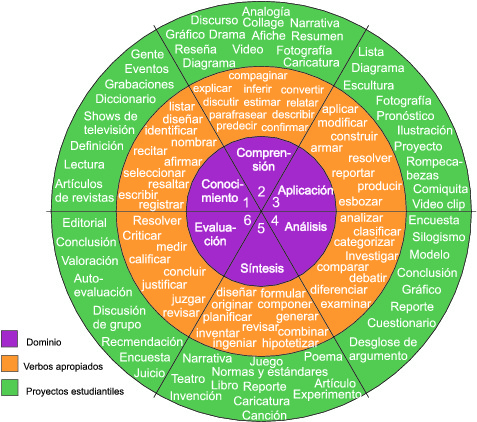
\includegraphics[height=12cm]{\OutputFigsDir/Bloom}
\label{fig:BloomTaxonomy}
\caption{Taxonomía de Bloom}
\end{figure} 
 %MH
\section{Perfil del ingresante}

El aspirante a ingresar a la \SchoolFullName de la \University debe tener:

\noindent Conocimientos de:
\begin{enumerate}
\item La operación básica de una computadora.
\item Conceptos básicos de operaciones algebraicas, geometría y precálculo.
\item Su entorno social en la actualidad.
\end{enumerate}

\noindent Habilidades para:
\begin{enumerate}
\item Entender las relaciones entre los hechos y encontrar las causas que los produjeron, prever consecuencias y así poder resolver problemas de una manera coherente.
\item Diferenciar patrones, es decir, captar la diferencia entre la realidad observada y el modelo mental o idea preconcebida que se ha tenido.
\item Percibir las relaciones lógicas (de funcionamiento o de comportamiento) existentes entre las observaciones realizadas.
\item Expresarse de manera oral o escrita las posibles soluciones para un problema dado.
\item Concentrarse y apertura al esfuerzo.
\item Comprender, analizar y sintetizar.
\item Formar hábitos y métodos adecuados para el estudio.
\end{enumerate}

\noindent Actitudes de:
\begin{enumerate}
\item Interés y gusto por el estudio de ciencia de la computación y matemáticas.
\item Disposición para el trabajo académico, en forma cooperativa y participativa, dentro y fuera del aula de clases.
\item Iniciativa y competencia en el desempeño escolar.
\end{enumerate}
 %YS
\section{Perfil del egresado}

El egresado del Programa Profesional de Ciencia de Datos es capaz de:
\begin{enumerate}
\item Entender la relación entre las matemáticas, la estadistica y la computación.
\item Desarrollar proyectos que abarcan todos los aspectos del manejo y análisis de datos.
\item Descifrar grandes volúmenes de datos, con el objetivo de descubrir tendencias y obtener una visión de los datos de tal manera que se evidencie su verdadero significado.
%% De CS:
\item Desarrollar tecnología computacional buscando el bien común de los individuos, la sociedad y las organizaciones.
\item Aportar con su formación humana y sus capacidades científicas y profesionales con la solución de los problemas sociales de nuestro entorno.
\item Transformar, acelerar y ampliar los límites de cualquier área del conocimiento a través de soluciones innovadoras basadas en el uso eficiente de tecnología computacional.
\item Incrementar las ventajas competitivas de cualquier organización a través del manejo eficiente de los datos.
\item Poder seguir estudios de postgrado con exigencia internacional en áreas relacionadas.
\end{enumerate}
  %YS
\section{Objetivos educacionales}\label{sec:educational-objectives}
Después de cinco años de egresado de la carrera profesional de Ciencia de la Computación, nuestros profesionales deben ser capaces de:
\begin{enumerate}
\item Tener suficiente entendimiento del campo incluyendo análisis de técnicas modernas y principios científicos de lo que desarrolla.
\item Demostrar liderazgo y capacidad de adaptación al cambio siendo promovido a una mejor posición dentro de la organización.
\item Demostrar un entendimiento de las implicancias éticas, legales, culturales, ambientales y económicas de lo que desarrolla.
\item Demostrar un entendimiento del impacto de todo lo que desarrolla en individuos, organizaciones e instituciones.
\item Aplicar de forma visible sus habilidades de comunicación con colegas de otras áreas, trabajo en equipo e interdisciplinario.
\item Involucrarse de forma efectiva en el desarrollo del equipo siendo mentor, aprendiendo de forma continua y autónoma.
\item Involucrarse en sociedades profesionales del área.
\end{enumerate}
 %MH
\section{Perfil del docente}
El docente de la \SchoolFullName de la \University es una persona que promueve la formación 
integral del estudiante a través de la enseñanza, la investigación y extensión, 
transmitiendo su sólidos conocimientos en los cursos que imparte fortaleciendo sus valores como persona y miembro de la sociedad.

Debe ser capaz de transmitir sus conocimientos de una forma simple y clara a los estudiantes 
fomentando en ellos la investigación continúa para que sean capaces de adaptarse fácilmente a los 
cambios tecnológicos y promover en ellos la búsqueda del bien común de los individuos, la sociedad y 
las organizaciones.

Debe ser un profesional que busca con frecuencia capacitación y grados académicos avanzados con el objetivo de desplegarse mejor hacia los individuos, las organizaciones y la sociedad.

El docente participa de la formación e integración del estudiante a una comunidad académica católica buscando siempre la exigencia continua.
\OnlyIS{\input{\InTexDir/IS-Capabilities-and-Knowledgement}}
\section{Grados y Títulos}\label{sec:cs-grados-y-titulos}
Cumplida la aprobación de los créditos académicos propuestos en la malla curricular 
y luego de haber cumplido con los requisitos estipulados en el reglamento de grados y 
títulos de la carrera, el egresado recibirá:

\AcademicDegreeAndTitle

% Considerando la participación de Miembros del Directorio de Actividades Educativas (\textit{Education Activities Board}) de IEEE a nivel mundial, este grupo de trabajo recomienda que no se utilice la palabra ingeniería en el nombre, pues esta carrera no es parte de la Ingeniería y ese es exactamente uno de los pilares que sustentan esta carrera. %YS
\section{Recursos para dictado de clases}\label{sec:resources-to-teach}
Un profesional innovador debe estar al tanto de los últimos avances de su área siempre. Los últimos avances de esta área no son presentados en los libros necesariamente. Debemos utilizar publicaciones de revistas indexadas de circulación mundial. Por esa razón tomamos como base la suscripción institucional a la ACM y a la IEEE-CS. Es recomendado que el docente use este material para discutir en clase las tendencias en todas las áreas.

Los laboratorios de cómputo también deben ser renovados de acuerdo a la rapidez
propia de esta área y esto implica renovaciones constantes para poder garantizar
que los estudiantes estén actualizados.
El recurso f­sico en cuanto a laboratorios para cada curso está detallado en el Capítulo \ref{chap:laboratorios}.
 %JB
%\input{\InInstitutionDir/example}
}

\OnlyPeruUNSA{
La computación ha sufrido un desarrollo impresionante en las últimas décadas, convirtiéndose en 
el motor del desarrollo científico, tecnológico, industrial, social, económico y cultural, 
transformando de manera significativa nuestro diario accionar.

El surgimiento del computador ha marcado una nueva era en la historia de la humanidad que era 
imposible de imaginar varias décadas atrás. La gran cantidad de aplicaciones que se han desarrollado 
en los últimos años están transformando el desarrollo de todas las disciplinas del saber, 
la comercialización en el ámbito globalizado en que vivimos, la manera en que nos comunicamos, 
los procesos de enseñanza-aprendizaje y hasta en la manera como nos entretenemos.

Para darnos una idea de la relevancia e importancia, que en nuestro país ha alcanzado esta 
disciplina, basta mencionar que actualmente se ofrecen aproximadamente más de 110 carreras de Computación a nivel nacional. 
Esto sin considerar los programas de nivel Técnico Superior No Universitario que se ofertan.

Todas estas carreras existentes tienen como centro de su estudio a la computación pero lo 
hacen con 28 nombres distintos como: Ingeniería de Sistemas, Ingeniería de Computación, 
Ingeniería de Computación y Sistemas, entre otros. A pesar de que todas ellas apuntan al mismo 
mercado de trabajo, resulta por lo menos sorprendente que no sea posible encontrar por lo menos dos 
que compartan la misma curricula.

Muchos países consideran a la computación como estratégica para su desarrollo. En Perú, 
el \ac{CONCYTEC} ha recomendado al gobierno que considere a la Computación como una de las 
áreas prioritarias de vinculación entre la academia e industria para fomentar la 
competitividad y la innovación.

Comúnmente, durante la década de los setenta, la Computación se desarrolló dentro 
de las Facultades de Ciencias en la mayoría de las universidades estadounidenses, 
británicas y de otros países. Durante la década de los ochenta, los grupos de 
computación en las universidades se esforzaron por lograr una legitimidad académica 
en su ámbito local. Frecuentemente, se transformaron en departamentos de Matemáticas y 
Computación, hasta finalmente dividirse en dos departamentos de Matemáticas y de 
Computación, en la década de los noventa. Es en esta década en que un número 
creciente de instituciones reconocieron la influencia penetrante de la Computación, 
creando unidades independientes como departamentos, escuelas o institutos dedicados a 
tal área de estudio, un cambio que ha demostrado tanto perspicacia como previsión. 

En Perú, un número cada vez mayor de instituciones de educación superior han 
tratado de seguir el desarrollo de las universidades extranjeras (aunque no siempre en 
forma muy seria o exitosa), reconociendo a la Computación como un área de estudio 
en sí misma, así como su importancia estratégica en la educación, y creando 
departamentos, escuelas o institutos dedicados a su estudio. La Facultad de \FacultadName 
no puede ser la excepción a este cambio, en el que ya se tiene un retraso relativo con 
muchas de las instituciones educativas dentro y fuera de Perú.

\section{Base Legal}
La \SchoolFullName fue creada según Resolución de Asamblea Universitaria Nro 006-2008, con fecha 02 de Octubre de 2008.
Así mismo, forma parte de la Estructura Academica de la \FacultadName de la \University.

\section{Base axiológica de la carrera}
Como la ciencia computación, es la disciplina que se dedica a la obtención y aplicación del conocimiento, 
los valores epistáamicos se consideran, entonces, valores internos o constitutivos a la ciencia de la computación, 
mientras que el resto de valores de diversos tipos se consideran externos.

El estudio de la ciencia de la computación se desarrolla como una gran oportunidad para resolver los grandes retos que la humanidad enfrenta  en el presente y el futuro.

La Axiología Computacional, está comprendida  por los siguientes indicadores de valor: el rendimiento, 
costos vs rendimiento, costos vs robustez,  compatibilidad, innovación, creatividad,  aplicaciones 
concretas a la solución de problemas de la sociedad,  transparencia, y calidad.

\section{Diagnóstico General}

\subsection{Análisis de Currículos}
Nuestra \SchoolFullName inicia sus actividades el 2010 con un currículo basado en la propuesta internacional de 
Ciencia de la Computación de IEEE y ACM en su versión 2008 \cite{ComputerScience2008}.

Esta propuesta ha permitido que nuestros alumnos sean formados de acuerdo a las recomendaciones internacionales para esta línea
siendo su formación compatible con lo que se enseña a nivel mundial.

Además, el hecho de estar alineados a una propuesta internacional facilita enormemente la movilidad estudiantil y de docentes,
el acceso a estudios de postgrado en el extranjero, la acreditación internacional. Todos estos son factores muy importantes en el 
desarrollo académico y profesional de una Escuela Profesional tan dinámica como lo es la computación hoy en dia.

A nivel internacional la siguiente propuesta para el área de Ciencia de la Computación fue publicada en el documento \cite{CS2013} donde 
inclusive uno de nuestros profesores participó en la elaboración de dicho documento como miembro del comité internacional que la formuló.

Este último documento \cite{CS2013} y el Curriculo de inicial de 2010 sirvieron como insumos para el presente currículo 
por lo cual estamos seguros que está totalmente actualizado con relación a las tendencias internacionales del área.

\subsection{Propuestas curriculares de la Escuela en otras universidades nacionales y extranjeras}
La referencia más sólida a nivel mundial en cuanto a la propuesta de carreras de 
computación para nivel de pregrado es la que fue propuesta en conjunto por la 
\ac{ACM}, \ac{IEEE-CS} y la \ac{AIS}. Estas tres organizaciones propusieron la 
Computing Curricula en el documento denominado: {\it Joint Task Force for Computing Curricula 2005, 
Computing Curricula 2005. Overview Report}\cite{ComputingCurricula2005}.

La \acl{CC} es un término de origen estadounidense \ac{CS}. Este término es 
conocido también como informática en el ámbito europeo\footnote{El término 
europeo es derivado del vocablo francés {\it Informatique}.}.

Según el diccionario de la Real Academia de la Lengua Española (http://www.rae.es) 
ambos términos también son sinónimos.

A nivel internacional, la computación presenta 5 perfiles claramente definidos: 
\begin{itemize}
\item Ciencia de la Computación (\textit{Computer Science}) \\ \cite{CS2013},
\item Ingeniería de Computación (\textit{Computer Engineering}) \cite{ComputerEngineering2004},
\item Sistemas de Información (\textit{Information Systems}) \cite{InformationSystemsCurricula2010, InformationSystems2002Journal},
\item Ingeniería de Software (\textit{Software Engineering}) \cite{SoftwareEngineering2004},
\item Tecnología de la Información (\textit{Information Technology}) \cite{InformationTechnology2005}
\end{itemize}

La Figura \ref{fig.cs} es tomada de la definición propuesta en la \textit{Computing Curricula} 
\cite{ComputingCurricula2005} en el área de \ac{CC} cuyo última versión es la denominada CS2013 (cs2013.org) \cite{CS2013}.
La \ac{CC} cubre la mayor parte entre el extremo superior y el extremo inferior, porque el 
profesional en \ac{CC} no trata ``solamente con el hardware'' que utiliza un software o de 
``solamente la organización'' que hace uso de la información que la computación le puede proveer. 

\begin{figure}[ht]
   \centering
   \includegraphics[width=13cm]{\OutputFigsDir/\currentarea}
   \caption{Campo acción de la Ciencia de la Computación}
   \label{fig.cs}
\end{figure}

%\begin{quote}
Las Ciencias de la Computación cubren un amplio rango, desde sus fundamentos teóricos y algorítmicos hasta 
los \'ultimos desarrollos en robótica, visión por computadora, sistemas inteligentes, bioinformática, y 
otras áreas emocionantes. Podemos pensar que el trabajo de un científico de la computación pertenece 
a las siguientes tres categorías:

\begin{itemize}
\item \textbf{Diseño e implementación de software}. Los científicos de computación se encargan de 
desafiantes labores de programación. También supervisan otros programadores, haciéndolos concientes 
de nuevas aproximaciones.

\item \textbf{Instrumentación de nuevas formas para usar computadoras}. El progreso en las áreas 
de ciencias de la computación como redes, bases de datos, e interfaces humano-computadora permitieron 
el desarrollo de la www y actualmente se trabaja en el desarrollo de metasistemas Grid. Además, 
los investigadores trabajan ahora en hacer que los robots sean ayudantes prácticos y demuestren 
inteligencia, utilizan las bases de datos para crear nuevos conocimientos, y están utilizando 
computadoras para decifrar los secretos de nuestro ADN.

\item \textbf{Desarrollo de formas efectivas de resolver problemas de computación.} 
Por ejemplo, los científicos de la computación desarrollan las mejores formas posibles 
de almacenar información en bases de datos, enviar datos a través de la red, y 
desplegar imágenes complejas. Sus bases teóricas les permiten determinar el 
mejor desempeño posible, y su estudio de algoritmos les ayuda a desarrollar 
nuevas aproximaciones para proveer un mejor desempeño.
\end{itemize}

Las Ciencias de la Computación cubren todo el rango desde la teoría hasta la programación. Mientras otras disciplinas pueden producir titulados mejor preparados para trabajos específicos, las ciencias de la computación ofrecen un amplio fundamento que permite a sus titulados adaptarse a nuevas tecnologías y nuevas ideas.
%\end{quote}

El profesional en \ac{CC} se preocupa por casi todo en medio de estas áreas. En dirección hacia el hardware, este profesional llega a desarrollar software que permite el funcionamiento de dispositivos {\it devices}. En dirección a aspectos organizacionales, el profesional de \ac{CC} ayuda a que los sistemas de información operen correctamente en las organizaciones. Él genera la tecnología que permite que otras áreas como los sistemas de información se desarrollen adecuadamente.

El profesional en \ac{CC} diseña y desarrolla todo tipo de software, desde infraestructura de plataformas (sistemas operativos, programas de comunicación, etc.) hasta aplicación de tecnologías (navegadores de Internet, bases de datos, motores de búsqueda, etc.). Este profesional crea estas capacidades, pero no está orientado al uso de las mismas. Por lo tanto, el área sombreada (fig. \ref{fig.cs}) para \ac{CC} se estrecha y finaliza en la medida que nos movamos hacia la aplicación y configuración de productos.


\subsection{Diagnóstico específico para la carrera}

\subsubsection{Los grandes retos en el desarrollo de la carrera profesional}
Uno de los caminos que se espera del área de computación en nuestro país pueda producir software a gran escala como las 
grandes empresas productoras de software a nivel mundial y convertirse en referente a nivel nacional, luego latinoamericano y 
finalmente a nivel mundial. En el ámbito de la computación, es común observar que los países cuentan con
Asociaciones de Productores de Software cuyas políticas están orientadas a la exportación. Siendo así, 
no tendría sentido preparar a nuestros alumnos sólo para el mercado local o nacional. 
Siendo un reto que nuestros egresados deben estar preparados para desenvolverse en el mundo globalizado que nos ha tocado vivir.

Es necesario recordar que la mayor innovación de productos comerciales de versiones recientes utiliza tecnología que se conocía 
en el mundo académico hace 20 años o más. Un ejemplo claro son las bases de datos que soportan datos y consultas espaciales 
desde hace muy pocos años. Sin embargo, utilizan estructuras de datos que ya existían hace algunas décadas. 
Es lógico pensar que la gente del área académica no se dedique a estudiar en profundidad la última versión de un 
determinado software cuando esa tecnología ya la conocían hace mucho tiempo. Por esa misma razón es raro en el 
mundo observar que una universidad tenga convenios con una transnacional de software para dictar solamente esa 
tecnología pues, nuestra función es generar esa tecnología y no sólo saber usarla.

\subsubsection{Aporte al desarrollo de las personas, instituciones y sociedad}
Nuestros futuros profesionales deben estar orientados a crear nuevas empresas de base tecnológica que puedan 
incrementar las exportaciones de software peruano. Este nuevo perfil está orientado a generar industria innovadora. 
Si nosotros somos capaces de exportar software competitivo también estaremos en condiciones de atraer nuevas inversiones. 
Las nuevas inversiones generarían más puestos de empleo bien remunerados y con un costo bajo en relación a otros tipos de industria. 
Bajo esta perspectiva, podemos afirmar que esta carrera será un motor que impulsará al desarrollo del país de forma decisiva 
con una inversión muy baja en relación a otros campos.

Tampoco debemos olvidar que los alumnos que ingresan hoy saldrán al mercado dentro de 5 años aproximadamente y, 
en un mundo que cambia tan rápido, no podemos ni debemos enseñarles tomando en cuenta solamente el mercado actual. 
Nuestros profesionales deben estar preparados para resolver los problemas que habrá dentro de 10 o 15 años y 
eso sólo es posible a través de la investigación en los diferentes problemas de nuestra región.


\subsubsection{Empleabilidad de egresados}
Nuestro egresado podrá prestar sus servicios profesionales en empresas e instituciones públicas y privadas que requieran 
sus capacidades en función del desarrollo que oferta, entre ellas:

\begin{itemize}
\item Empresas dedicadas a la producción de software con calidad internacional.
\item Empresas, instituciones y organizaciones que requieran software de calidad para mejorar sus actividades y/o servicios ofertados.
\end{itemize}


Nuestro egresado puede desempeñarse en el mercado laboral sin ningún problema ya que, en general, la exigencia del 
mercado y campo ocupacional está más orientada al uso de herramientas. Sin embargo, es poco común que los propios 
profesionales de esta carrera se pregunten: ?`qué tipo de formación debería tener si yo quisiera crear esas herramientas además de saber usarlas?.  
Ambos perfiles (usuario y creador) son bastante diferentes pues no sería posible usar algo que todavía no fue creado. 
En otras palabras, los creadores de tecnología son los que dan origen a nuevos puestos de trabajo y abren 
la posibilidad de que otros puedan usar esa tecnología.

Debido a la formación basada en la investigación, nuestro profesional debe siempre ser un innovador donde trabaje. 
Esta misma formación permite que el egresado piense también en crear su propia empresa de desarrollo de software. 
Considerando que países como el nuestro tienen un costo de vida mucho menor que Norte América ó Europa, una 
posibilidad que se muestra interesante es la exportación de software pero eso requiere que la calidad del 
producto sea al mismo nivel de lo ofrecido a nivel internacional.

Este perfil profesional también posibilita que nuestros egresados se queden en nuestro país; 
producir software en nuestro país y venderlo fuera es más rentable que salir al extranjero y comercializarlo allá.

El campo ocupacional de un egresado es amplio y están en continua expansión y cambio. 
Prácticamente toda empresa u organización hace uso de servicios de computación de algún tipo, y la buena 
formación básica de nuestros egresados hace que puedan responder a los requerimientos de las mismas exitosamente. 
Este egresado, no sólo podrá dar soluciones a los problemas existentes sino que deberá proponer innovaciones 
tecnológicas que impulsen la empresa hacia un progreso constante.

A medida que la informatización básica de las empresas del país avanza, la necesidad de personas capacitadas 
para resolver los problemas de mayor complejidad aumenta y el plan de estudios que hemos desarrollado tiene 
como objetivo satisfacer esta demanda considerándola a mediano y largo plazo. El campo para las tareas de 
investigación y desarrollo de problemas complejos en computación es también muy amplio y están creciendo día a día a nivel mundial.

Debido a la capacidad innovadora de nuestro egresado, existe una mayor la probabilidad de registrar 
patentes con un alto nivel inventivo lo cual es especialmente importante en nuestros países.

\subsubsection{Competencias requeridas para el mercado laboral}
En un área tan globalizada como lo es la computación el mercado laboral no podría ser solamente local o nacional.
Hoy en dia, en Arequipa, es posible observar empresas de la India, de California, de Alemania, de Uruguay que operan desde nuestra ciudad.
Esto obliga a que la preparación de nuestros egresados tenga que ser competitiva a nivel mundial.

También existen aquellos defensores de que el Perú debe formar profesionales en esta área solo para problemas locales.
Sin embargo, consideramos que es una de las razones de nuestro atraso pues continuamos siendo un país de usuarios de 
tecnología pero no podemos producirla con calidad internacional aun debido al número muy reducido de profesional con perfil internacional. 

Un análisis muy reciente al respecto que nos ayuda a entender mejor como Perú es observado desde fuera puede ser visto en un 
artículo reciente publicado en Boston\footnote{http://bit.ly/2i5lzNM} por el Mag Eddy Wong.
En esta publicación de indica de forma clara que las universidades peruanas han venido formando solamente usuarios de tecnología y 
que además existe un énfasis en mantener asociada la palabra Ingeniería a estas carreras.
Esta formación de usuarios crea una dependencia enorme de nuestro país y dificulta enormemente el desarrollo de la industria nacional.
Es cierto que existen más de 100 carreras de esta línea pero los profesionales unicamente son orientados a hacer uso de la tecnología que es importada a nuestro país.
De parte de las empresas del sector de software existe mucha dificultad para encontrar personal capacitado para crear software de calidad internacional.
Esto puede ser corroborado directamente con el Presidente de la Asociación Peruana de Productores de Software (APESOFT) 
quien con frecuencia reclama este problema al ámbito académico.

\subsubsection{Situación de egresados}
La primera promoción egreso a inicios de 2015 con un total de 6 egresados los cuales fueron aceptados en su totalidad 
para ir a estudiar maestrías con beca a Brasil en área de Ciencia de la Computación.
El hecho de sea el 100\% de egresados en esta situación es un reflejo claro del nivel que se ha podido alcanzar a 
pesar de las dificultades propias de una universidad nacional en nuestro país.
En este momento estos 6 alumnos ya están culminando con éxito sus estudios de maestría e iniciando los de doctorado.

La segunda promoción egresó a inicios de 2016 con un aproximado de 8 alumnos que han seguido un camino similar al primer 
grupo estudiando maestrías becados por concurso a tiempo completo en Arequipa, Holanda, y Brasil.

Estos niveles de competitividad no habrían sido posibles si la formación hubiese sido de usuarios o 
solamente orientada al mercado local o nacional. 

Las competencias que más destacan en nuestros egresados son:
\begin{itemize}
\item Habilidad aprender a aprender de forma autónoma,
\item Capacidad de adaptación rápida a grupos de investigación de nivel internacional,
\item Capacidad de adaptación rápida al trabajo con nuevas tecnologías,
\item Competencia para trabajo multidisciplinario,
\item Competencia para comunicarse de forma efectiva en inglés y en varios casos también en portugues.
\end{itemize}

Como varios de nuestros alumnos han salido a otros países, es nuestra responsabilidad que tengan el 
espacio adecuado en nuestro medio para poder integrarlos y mejorar la calidad académica existente.

\subsubsection{Oportunidades de empleo}
Nuestro egresado podrá prestar sus servicios profesionales en empresas e instituciones públicas y privadas 
que requieran sus capacidades en función del desarrollo que oferta, entre ellas:

\begin{itemize}
\item Empresas dedicadas a la producción de software con calidad internacional.
\item Empresas, instituciones y organizaciones que requieran software de calidad para mejorar sus actividades y/o servicios ofertados.
\end{itemize}

Nuestro egresado puede desempeñarse en el mercado laboral sin ningún problema ya que, en general, la 
exigencia del mercado y campo ocupacional está mucho más orientada al uso de herramientas. Sin embargo, 
es poco común que los propios profesionales de esta carrera se pregunten: ?`qué tipo de formación debería 
tener si yo quisiera crear esas herramientas además de saber usarlas?. Ambos perfiles (usuario y creador) 
son bastante diferentes pues no sería posible usar algo que todavía no fue creado. En otras palabras, 
los creadores de tecnología son los que \underline{dan origen a nuevos puestos de trabajo} y abren la 
posibilidad de que otros puedan usar esa tecnología.

Debido a la formación basada en la investigación, nuestro profesional debe siempre ser un innovador 
donde trabaje. Esta misma formación permite que el egresado piense también en crear su propia empresa 
de desarrollo de software. Considerando que países como el nuestro tienen un costo de vida mucho menor 
que Norte América ó Europa, una posibilidad que se muestra interesante es la exportación de software 
pero eso requiere que la calidad del producto sea al mismo nivel de lo ofrecido a nivel internacional.

Este perfil profesional también posibilita que nuestros egresados se queden en nuestro país; producir 
software en nuestro país y venderlo fuera es más rentable que salir al extranjero y comercializarlo allá.

El campo ocupacional de un egresado es amplio y está en continua expansión y cambio. Prácticamente 
toda empresa u organización hace uso de servicios de computación de algún tipo, y la buena formación 
básica de nuestros egresados hace que puedan responder a los requerimientos de las mismas exitosamente. 
Este egresado, no sólo podrá dar soluciones a los problemas existentes sino que deberá proponer innovaciones 
tecnológicas que impulsen la empresa hacia un progreso constante.

A medida que la informatización básica de las empresas del país avanza, la necesidad de personas 
capacitadas para resolver los problemas de mayor complejidad aumenta y el plan de estudios que hemos 
desarrollado tiene como objetivo satisfacer esta demanda considerandola a mediano y largo plazo. El campo 
para las tareas de investigación y desarrollo de problemas complejos en computación es también muy amplio 
y está creciendo día a día a nivel mundial.

Debido a la capacidad innovadora de nuestro egresado, existe una mayor la probabilidad de registrar 
patentes con un alto nivel inventivo lo cual es especialmente importante en nuestros países.


% \subsubsection{Aporte al desarrollo del conocimiento}
% Las necesidades de los Científicos e Ingenieros con relación a computación han impulsado mucho la 
% investigación y la innovación en computación. A medida que las computadoras aumentan su poder en la 
% solución de problemas, la ciencia computacional ha crecido tanto en amplitud e importancia. 
% Es una disciplina por derecho propio y se considera que es una de las cinco con mayor crecimiento.
% Una increíble variedad de sub-campos han surgido bajo el paraguas de la Ciencia Computacional, 
% incluyendo la biología computacional, química computacional, mecánica computacional, 
% arqueología computacional, finanzas computacionales, sociología computacional y forense.

\section{Estrategias de Enseñanza-Aprendizaje}
El avance progresivo de las tecnologías y redes móviles, habilita nuevas herramientas para ser exploradas y 
experimentadas en escenarios de aprendizaje. Es así, como el uso de dispositivos móviles, añade nuevas 
dimensiones al proceso de enseñanza aprendizaje, como la movilidad y personalización. La evolución de los 
componentes de E-Learning (aprendizaje soportado por medios electrónicos) para el aprendizaje móvil y aprendizaje ubicuo, 
abre el espacio conceptual y técnico para el desarrollo de la Internet de los objetos (IoT), de sus siglas en inglés de {\it Internet of Things}, en el aprendizaje.

La tendencia generalizada de parte de los estudiantes a aceptar positivamente las herramientas que 
impliquen una novedad en el proceso de enseñanza-aprendizaje, nos indica que la inclusión de elementos nuevos, es favorable para el ánimo frente al aprendizaje.

Teniendo en cuenta que las actividades intensivas en cuanto al uso de dispositivos especializados, 
deben ser cuidadosamente diseñadas, sobre todo en cuanto a imprudencias o excesos de parte de los usuarios, 
lo cual puede llevar a fallas y posibles pérdidas de información, entonces podemos hacer uso de IoT 
para hacer más agradable el proceso de aprendizaje.

Por lo que, consideramos implementar los siguientes conceptos estratégicos:

\begin{itemize}
\item Horizontalidad educativa.
\item Material audiovisual, aprendamos con documentales y con todo lo que nos da hoy la tecnología.
\item interactividad grupal.
\item Motivación de la curiosidad.
\item Fomento de la creatividad.
\item Pensamiento lateral.
\item Uso adecuado de las tecnologías.
\item Autoaprendizaje guiado.
\item Estimulación de la inteligencia en lugar de estimular la memoria.
\item Diversión incorporada, mientras aprendemos ó enseñamos.
\end{itemize}
\section{Elementos Institucionales}

\begin{itemize}
 
\item \textbf{Alumnos Pre-grado}
\begin{itemize}
\item Cantidad de Alumnos Matriculados 225
\item Cantidad de Egresados 22
\item Cantidad de Graduados Bachilleres 8
\end{itemize} 

\item \textbf{Docentes}
\begin{itemize}
\item Principal Tiempo Completo Nombrado: 1
\item Asociado Tiempo Completo Nombrado: 1
\item Asociado Tiempo Parcial (20 Horas) Nombrado: 1
\item Auxiliar Tiempo Parcial (20 Horas) Nombrado: 1
\item Auxiliar Tiempo Parcial (20 Horas) Contratado: 1
\item Auxiliar Tiempo Parcial (10 Horas) Nombrado: 3
\item Auxiliar Tiempo Completo Nombrado: 1
\item Auxiliar Tiempo Completo Contratado: 1
\end{itemize} 

\item \textbf{Administrativos}
\begin{itemize}
\item Personal en secretaria contratado: 1
\end{itemize}

\item \textbf{Infraestructura y Equipos}
\begin{itemize}
\item Número de Aulas: 2
\item Número de Oficinas Administrativas: 1
\item Número de Laboratorios: 2
\item Número de computadoras: 41
\item Número de cañones multimedia: 4 
\item Número de Laptops: 4
\item Número de Impresoras: 1
\end{itemize}

\end{itemize}


\section{Perfil del egresado}

El egresado del Programa Profesional de Ciencia de Datos es capaz de:
\begin{enumerate}
\item Entender la relación entre las matemáticas, la estadistica y la computación.
\item Desarrollar proyectos que abarcan todos los aspectos del manejo y análisis de datos.
\item Descifrar grandes volúmenes de datos, con el objetivo de descubrir tendencias y obtener una visión de los datos de tal manera que se evidencie su verdadero significado.
%% De CS:
\item Desarrollar tecnología computacional buscando el bien común de los individuos, la sociedad y las organizaciones.
\item Aportar con su formación humana y sus capacidades científicas y profesionales con la solución de los problemas sociales de nuestro entorno.
\item Transformar, acelerar y ampliar los límites de cualquier área del conocimiento a través de soluciones innovadoras basadas en el uso eficiente de tecnología computacional.
\item Incrementar las ventajas competitivas de cualquier organización a través del manejo eficiente de los datos.
\item Poder seguir estudios de postgrado con exigencia internacional en áreas relacionadas.
\end{enumerate}

  \subsection{Competencias Generales del profesional en Computación}
De acuerdo al más reciente publicación en este aspecto \cite{IEEECompetences}, las competencias generales para los profesionales de computación son las siguientes:

\begin{enumerate}
\renewcommand{\theenumi}{C\arabic{enumi}}
\item \Competence{C1}
\item \Competence{C2}
\item \Competence{C3}
\item \Competence{C4}
\item \Competence{C5}
\item \Competence{C6}
\item \Competence{C7}
\item \Competence{C8}
\item \Competence{C9}
\item \Competence{C10}
\item \Competence{C11}
\item \Competence{C12}
\item \Competence{C13}
\item \Competence{C14}
\item \Competence{C15}
\item \Competence{C16}
\item \Competence{C17}
\item \Competence{C18}
\item \Competence{C19}
\item \Competence{C20}
\item \Competence{C21}
\item \Competence{C22}
\item \Competence{C23}
\item \Competence{C24}
\item \Competence{C25}
\end{enumerate}
  \subsection{Competencias Específicas para Ciencia de la Computación (\textit{Computer Science})}
En la carrera de Ciencia de la Computación (\textit{Computer Science}) \cite{CS2013}, las competencias específicas son \cite{IEEECompetences}:

\begin{enumerate}
\renewcommand{\theenumi}{CS\arabic{enumi}}
\item \Competence{CS1}
\item \Competence{CS2}
\item \Competence{CS3}
\item \Competence{CS4}
\item \Competence{CS5}
\item \Competence{CS6}
\item \Competence{CS7}
\item \Competence{CS8}
\item \Competence{CS9}
\item \Competence{CS10}
\item \Competence{CS11}
\item \Competence{CS12}
\end{enumerate}

}


% % %\part{Otra parte}
%\chapter{Cuerpo del conocimiento de Ciencia de la Computación}\label{chap:BOK}
\noindent 
Las 18 principales áreas de conocimiento en Ciencia de la Computación son:

\begin{multicols}{2}
\scriptsize
\noindent
\textbf{\ref{sec:BOK:AL} \htmlref{\AL}{sec:BOK:AL}\xspace (Pág.~\pageref{sec:BOK:AL})}
\begin{itemize}
\item \ref{sec:BOK:ALBasicAnalysis} \htmlref{\ALBasicAnalysis}{sec:BOK:ALBasicAnalysis}\xspace (Pág.~\pageref{sec:BOK:ALBasicAnalysis})
\item \ref{sec:BOK:ALAlgorithmicStrategies} \htmlref{\ALAlgorithmicStrategies}{sec:BOK:ALAlgorithmicStrategies}\xspace (Pág.~\pageref{sec:BOK:ALAlgorithmicStrategies})
\item \ref{sec:BOK:ALFundamentalDataStructuresandAlgorithms} \htmlref{\ALFundamentalDataStructuresandAlgorithms}{sec:BOK:ALFundamentalDataStructuresandAlgorithms}\xspace (Pág.~\pageref{sec:BOK:ALFundamentalDataStructuresandAlgorithms})
\item \ref{sec:BOK:ALBasicAutomataComputabilityandComplexity} \htmlref{\ALBasicAutomataComputabilityandComplexity}{sec:BOK:ALBasicAutomataComputabilityandComplexity}\xspace (Pág.~\pageref{sec:BOK:ALBasicAutomataComputabilityandComplexity})
\item \ref{sec:BOK:ALAdvancedComputationalComplexity} \htmlref{\ALAdvancedComputationalComplexity}{sec:BOK:ALAdvancedComputationalComplexity}\xspace (Pág.~\pageref{sec:BOK:ALAdvancedComputationalComplexity})
\item \ref{sec:BOK:ALAdvancedAutomataTheoryandComputability} \htmlref{\ALAdvancedAutomataTheoryandComputability}{sec:BOK:ALAdvancedAutomataTheoryandComputability}\xspace (Pág.~\pageref{sec:BOK:ALAdvancedAutomataTheoryandComputability})
\item \ref{sec:BOK:ALAdvancedDataStructuresAlgorithmsandAnalysis} \htmlref{\ALAdvancedDataStructuresAlgorithmsandAnalysis}{sec:BOK:ALAdvancedDataStructuresAlgorithmsandAnalysis}\xspace (Pág.~\pageref{sec:BOK:ALAdvancedDataStructuresAlgorithmsandAnalysis})
\end{itemize}

\textbf{\ref{sec:BOK:AR} \htmlref{\AR}{sec:BOK:AR}\xspace (Pág.~\pageref{sec:BOK:AR})}
\begin{itemize}
\item \ref{sec:BOK:ARDigitallogicanddigitalsystems} \htmlref{\ARDigitallogicanddigitalsystems}{sec:BOK:ARDigitallogicanddigitalsystems}\xspace (Pág.~\pageref{sec:BOK:ARDigitallogicanddigitalsystems})
\item \ref{sec:BOK:ARMachinelevelrepresentationofdata} \htmlref{\ARMachinelevelrepresentationofdata}{sec:BOK:ARMachinelevelrepresentationofdata}\xspace (Pág.~\pageref{sec:BOK:ARMachinelevelrepresentationofdata})
\item \ref{sec:BOK:ARAssemblylevelmachineorganization} \htmlref{\ARAssemblylevelmachineorganization}{sec:BOK:ARAssemblylevelmachineorganization}\xspace (Pág.~\pageref{sec:BOK:ARAssemblylevelmachineorganization})
\item \ref{sec:BOK:ARMemorysystemorganizationandarchitecture} \htmlref{\ARMemorysystemorganizationandarchitecture}{sec:BOK:ARMemorysystemorganizationandarchitecture}\xspace (Pág.~\pageref{sec:BOK:ARMemorysystemorganizationandarchitecture})
\item \ref{sec:BOK:ARInterfacingandcommunication} \htmlref{\ARInterfacingandcommunication}{sec:BOK:ARInterfacingandcommunication}\xspace (Pág.~\pageref{sec:BOK:ARInterfacingandcommunication})
\item \ref{sec:BOK:ARFunctionalorganization} \htmlref{\ARFunctionalorganization}{sec:BOK:ARFunctionalorganization}\xspace (Pág.~\pageref{sec:BOK:ARFunctionalorganization})
\item \ref{sec:BOK:ARMultiprocessingandalternativearchitectures} \htmlref{\ARMultiprocessingandalternativearchitectures}{sec:BOK:ARMultiprocessingandalternativearchitectures}\xspace (Pág.~\pageref{sec:BOK:ARMultiprocessingandalternativearchitectures})
\item \ref{sec:BOK:ARPerformanceenhancements} \htmlref{\ARPerformanceenhancements}{sec:BOK:ARPerformanceenhancements}\xspace (Pág.~\pageref{sec:BOK:ARPerformanceenhancements})
\end{itemize}

\textbf{\ref{sec:BOK:DS} \htmlref{\DS}{sec:BOK:DS}\xspace (Pág.~\pageref{sec:BOK:DS})}
\begin{itemize}
\item \ref{sec:BOK:DSSetsRelationsandFunctions} \htmlref{\DSSetsRelationsandFunctions}{sec:BOK:DSSetsRelationsandFunctions}\xspace (Pág.~\pageref{sec:BOK:DSSetsRelationsandFunctions})
\item \ref{sec:BOK:DSBasicLogic} \htmlref{\DSBasicLogic}{sec:BOK:DSBasicLogic}\xspace (Pág.~\pageref{sec:BOK:DSBasicLogic})
\item \ref{sec:BOK:DSProofTechniques} \htmlref{\DSProofTechniques}{sec:BOK:DSProofTechniques}\xspace (Pág.~\pageref{sec:BOK:DSProofTechniques})
\item \ref{sec:BOK:DSBasicsofCounting} \htmlref{\DSBasicsofCounting}{sec:BOK:DSBasicsofCounting}\xspace (Pág.~\pageref{sec:BOK:DSBasicsofCounting})
\item \ref{sec:BOK:DSGraphsandTrees} \htmlref{\DSGraphsandTrees}{sec:BOK:DSGraphsandTrees}\xspace (Pág.~\pageref{sec:BOK:DSGraphsandTrees})
\item \ref{sec:BOK:DSDiscreteProbability} \htmlref{\DSDiscreteProbability}{sec:BOK:DSDiscreteProbability}\xspace (Pág.~\pageref{sec:BOK:DSDiscreteProbability})
\end{itemize}

\textbf{\ref{sec:BOK:GV} \htmlref{\GV}{sec:BOK:GV}\xspace (Pág.~\pageref{sec:BOK:GV})}
\begin{itemize}
\item \ref{sec:BOK:GVFundamentalConcepts} \htmlref{\GVFundamentalConcepts}{sec:BOK:GVFundamentalConcepts}\xspace (Pág.~\pageref{sec:BOK:GVFundamentalConcepts})
\item \ref{sec:BOK:GVBasicRendering} \htmlref{\GVBasicRendering}{sec:BOK:GVBasicRendering}\xspace (Pág.~\pageref{sec:BOK:GVBasicRendering})
\item \ref{sec:BOK:GVGeometricModeling} \htmlref{\GVGeometricModeling}{sec:BOK:GVGeometricModeling}\xspace (Pág.~\pageref{sec:BOK:GVGeometricModeling})
\item \ref{sec:BOK:GVAdvancedRendering} \htmlref{\GVAdvancedRendering}{sec:BOK:GVAdvancedRendering}\xspace (Pág.~\pageref{sec:BOK:GVAdvancedRendering})
\item \ref{sec:BOK:GVComputerAnimation} \htmlref{\GVComputerAnimation}{sec:BOK:GVComputerAnimation}\xspace (Pág.~\pageref{sec:BOK:GVComputerAnimation})
\item \ref{sec:BOK:GVVisualization} \htmlref{\GVVisualization}{sec:BOK:GVVisualization}\xspace (Pág.~\pageref{sec:BOK:GVVisualization})
\end{itemize}

\textbf{\ref{sec:BOK:HCI} \htmlref{\HCI}{sec:BOK:HCI}\xspace (Pág.~\pageref{sec:BOK:HCI})}
\begin{itemize}
\item \ref{sec:BOK:HCIFoundations} \htmlref{\HCIFoundations}{sec:BOK:HCIFoundations}\xspace (Pág.~\pageref{sec:BOK:HCIFoundations})
\item \ref{sec:BOK:HCIDesigningInteraction} \htmlref{\HCIDesigningInteraction}{sec:BOK:HCIDesigningInteraction}\xspace (Pág.~\pageref{sec:BOK:HCIDesigningInteraction})
\item \ref{sec:BOK:HCIProgrammingInteractiveSystems} \htmlref{\HCIProgrammingInteractiveSystems}{sec:BOK:HCIProgrammingInteractiveSystems}\xspace (Pág.~\pageref{sec:BOK:HCIProgrammingInteractiveSystems})
\item \ref{sec:BOK:HCIUsercentereddesignandtesting} \htmlref{\HCIUsercentereddesignandtesting}{sec:BOK:HCIUsercentereddesignandtesting}\xspace (Pág.~\pageref{sec:BOK:HCIUsercentereddesignandtesting})
\item \ref{sec:BOK:HCINewInteractiveTechnologies} \htmlref{\HCINewInteractiveTechnologies}{sec:BOK:HCINewInteractiveTechnologies}\xspace (Pág.~\pageref{sec:BOK:HCINewInteractiveTechnologies})
\item \ref{sec:BOK:HCICollaborationandcommunication} \htmlref{\HCICollaborationandcommunication}{sec:BOK:HCICollaborationandcommunication}\xspace (Pág.~\pageref{sec:BOK:HCICollaborationandcommunication})
\item \ref{sec:BOK:HCIStatisticalmethodsforHCI} \htmlref{\HCIStatisticalmethodsforHCI}{sec:BOK:HCIStatisticalmethodsforHCI}\xspace (Pág.~\pageref{sec:BOK:HCIStatisticalmethodsforHCI})
\item \ref{sec:BOK:HCIHumanfactorsandsecurity} \htmlref{\HCIHumanfactorsandsecurity}{sec:BOK:HCIHumanfactorsandsecurity}\xspace (Pág.~\pageref{sec:BOK:HCIHumanfactorsandsecurity})
\item \ref{sec:BOK:HCIDesignorientedHCI} \htmlref{\HCIDesignorientedHCI}{sec:BOK:HCIDesignorientedHCI}\xspace (Pág.~\pageref{sec:BOK:HCIDesignorientedHCI})
\item \ref{sec:BOK:HCIMixedAugmentedandVirtualReality} \htmlref{\HCIMixedAugmentedandVirtualReality}{sec:BOK:HCIMixedAugmentedandVirtualReality}\xspace (Pág.~\pageref{sec:BOK:HCIMixedAugmentedandVirtualReality})
\end{itemize}

\textbf{\ref{sec:BOK:IAS} \htmlref{\IAS}{sec:BOK:IAS}\xspace (Pág.~\pageref{sec:BOK:IAS})}
\begin{itemize}
\item \ref{sec:BOK:IASFoundationalConceptsinSecurity} \htmlref{\IASFoundationalConceptsinSecurity}{sec:BOK:IASFoundationalConceptsinSecurity}\xspace (Pág.~\pageref{sec:BOK:IASFoundationalConceptsinSecurity})
\item \ref{sec:BOK:IASPrinciplesofSecureDesign} \htmlref{\IASPrinciplesofSecureDesign}{sec:BOK:IASPrinciplesofSecureDesign}\xspace (Pág.~\pageref{sec:BOK:IASPrinciplesofSecureDesign})
\item \ref{sec:BOK:IASDefensiveProgramming} \htmlref{\IASDefensiveProgramming}{sec:BOK:IASDefensiveProgramming}\xspace (Pág.~\pageref{sec:BOK:IASDefensiveProgramming})
\item \ref{sec:BOK:IASThreatsandAttacks} \htmlref{\IASThreatsandAttacks}{sec:BOK:IASThreatsandAttacks}\xspace (Pág.~\pageref{sec:BOK:IASThreatsandAttacks})
\item \ref{sec:BOK:IASNetworkSecurity} \htmlref{\IASNetworkSecurity}{sec:BOK:IASNetworkSecurity}\xspace (Pág.~\pageref{sec:BOK:IASNetworkSecurity})
\item \ref{sec:BOK:IASCryptography} \htmlref{\IASCryptography}{sec:BOK:IASCryptography}\xspace (Pág.~\pageref{sec:BOK:IASCryptography})
\item \ref{sec:BOK:IASWebSecurity} \htmlref{\IASWebSecurity}{sec:BOK:IASWebSecurity}\xspace (Pág.~\pageref{sec:BOK:IASWebSecurity})
\item \ref{sec:BOK:IASPlatformSecurity} \htmlref{\IASPlatformSecurity}{sec:BOK:IASPlatformSecurity}\xspace (Pág.~\pageref{sec:BOK:IASPlatformSecurity})
\item \ref{sec:BOK:IASSecurityPolicyandGovernance} \htmlref{\IASSecurityPolicyandGovernance}{sec:BOK:IASSecurityPolicyandGovernance}\xspace (Pág.~\pageref{sec:BOK:IASSecurityPolicyandGovernance})
\item \ref{sec:BOK:IASDigitalForensics} \htmlref{\IASDigitalForensics}{sec:BOK:IASDigitalForensics}\xspace (Pág.~\pageref{sec:BOK:IASDigitalForensics})
\item \ref{sec:BOK:IASSecureSoftwareEngineering} \htmlref{\IASSecureSoftwareEngineering}{sec:BOK:IASSecureSoftwareEngineering}\xspace (Pág.~\pageref{sec:BOK:IASSecureSoftwareEngineering})
\end{itemize}

\textbf{\ref{sec:BOK:IM} \htmlref{\IM}{sec:BOK:IM}\xspace (Pág.~\pageref{sec:BOK:IM})}
\begin{itemize}
\item \ref{sec:BOK:IMInformationManagementConcepts} \htmlref{\IMInformationManagementConcepts}{sec:BOK:IMInformationManagementConcepts}\xspace (Pág.~\pageref{sec:BOK:IMInformationManagementConcepts})
\item \ref{sec:BOK:IMDatabaseSystems} \htmlref{\IMDatabaseSystems}{sec:BOK:IMDatabaseSystems}\xspace (Pág.~\pageref{sec:BOK:IMDatabaseSystems})
\item \ref{sec:BOK:IMDataModeling} \htmlref{\IMDataModeling}{sec:BOK:IMDataModeling}\xspace (Pág.~\pageref{sec:BOK:IMDataModeling})
\item \ref{sec:BOK:IMIndexing} \htmlref{\IMIndexing}{sec:BOK:IMIndexing}\xspace (Pág.~\pageref{sec:BOK:IMIndexing})
\item \ref{sec:BOK:IMRelationalDatabases} \htmlref{\IMRelationalDatabases}{sec:BOK:IMRelationalDatabases}\xspace (Pág.~\pageref{sec:BOK:IMRelationalDatabases})
\item \ref{sec:BOK:IMQueryLanguages} \htmlref{\IMQueryLanguages}{sec:BOK:IMQueryLanguages}\xspace (Pág.~\pageref{sec:BOK:IMQueryLanguages})
\item \ref{sec:BOK:IMTransactionProcessing} \htmlref{\IMTransactionProcessing}{sec:BOK:IMTransactionProcessing}\xspace (Pág.~\pageref{sec:BOK:IMTransactionProcessing})
\item \ref{sec:BOK:IMDistributedDatabases} \htmlref{\IMDistributedDatabases}{sec:BOK:IMDistributedDatabases}\xspace (Pág.~\pageref{sec:BOK:IMDistributedDatabases})
\item \ref{sec:BOK:IMPhysicalDatabaseDesign} \htmlref{\IMPhysicalDatabaseDesign}{sec:BOK:IMPhysicalDatabaseDesign}\xspace (Pág.~\pageref{sec:BOK:IMPhysicalDatabaseDesign})
\item \ref{sec:BOK:IMDataMining} \htmlref{\IMDataMining}{sec:BOK:IMDataMining}\xspace (Pág.~\pageref{sec:BOK:IMDataMining})
\item \ref{sec:BOK:IMInformationStorageandRetrieval} \htmlref{\IMInformationStorageandRetrieval}{sec:BOK:IMInformationStorageandRetrieval}\xspace (Pág.~\pageref{sec:BOK:IMInformationStorageandRetrieval})
\item \ref{sec:BOK:IMMultimediaSystems} \htmlref{\IMMultimediaSystems}{sec:BOK:IMMultimediaSystems}\xspace (Pág.~\pageref{sec:BOK:IMMultimediaSystems})
\end{itemize}

\textbf{\ref{sec:BOK:IS} \htmlref{\IS}{sec:BOK:IS}\xspace (Pág.~\pageref{sec:BOK:IS})}
\begin{itemize}
\item \ref{sec:BOK:ISFundamentalIssues} \htmlref{\ISFundamentalIssues}{sec:BOK:ISFundamentalIssues}\xspace (Pág.~\pageref{sec:BOK:ISFundamentalIssues})
\item \ref{sec:BOK:ISBasicSearchStrategies} \htmlref{\ISBasicSearchStrategies}{sec:BOK:ISBasicSearchStrategies}\xspace (Pág.~\pageref{sec:BOK:ISBasicSearchStrategies})
\item \ref{sec:BOK:ISBasicKnowledgeRepresentationandReasoning} \htmlref{\ISBasicKnowledgeRepresentationandReasoning}{sec:BOK:ISBasicKnowledgeRepresentationandReasoning}\xspace (Pág.~\pageref{sec:BOK:ISBasicKnowledgeRepresentationandReasoning})
\item \ref{sec:BOK:ISBasicMachineLearning} \htmlref{\ISBasicMachineLearning}{sec:BOK:ISBasicMachineLearning}\xspace (Pág.~\pageref{sec:BOK:ISBasicMachineLearning})
\item \ref{sec:BOK:ISAdvancedSearch} \htmlref{\ISAdvancedSearch}{sec:BOK:ISAdvancedSearch}\xspace (Pág.~\pageref{sec:BOK:ISAdvancedSearch})
\item \ref{sec:BOK:ISAdvancedRepresentationandReasoning} \htmlref{\ISAdvancedRepresentationandReasoning}{sec:BOK:ISAdvancedRepresentationandReasoning}\xspace (Pág.~\pageref{sec:BOK:ISAdvancedRepresentationandReasoning})
\item \ref{sec:BOK:ISReasoningUnderUncertainty} \htmlref{\ISReasoningUnderUncertainty}{sec:BOK:ISReasoningUnderUncertainty}\xspace (Pág.~\pageref{sec:BOK:ISReasoningUnderUncertainty})
\item \ref{sec:BOK:ISAgents} \htmlref{\ISAgents}{sec:BOK:ISAgents}\xspace (Pág.~\pageref{sec:BOK:ISAgents})
\item \ref{sec:BOK:ISNaturalLanguageProcessing} \htmlref{\ISNaturalLanguageProcessing}{sec:BOK:ISNaturalLanguageProcessing}\xspace (Pág.~\pageref{sec:BOK:ISNaturalLanguageProcessing})
\item \ref{sec:BOK:ISAdvancedMachineLearning} \htmlref{\ISAdvancedMachineLearning}{sec:BOK:ISAdvancedMachineLearning}\xspace (Pág.~\pageref{sec:BOK:ISAdvancedMachineLearning})
\item \ref{sec:BOK:ISRobotics} \htmlref{\ISRobotics}{sec:BOK:ISRobotics}\xspace (Pág.~\pageref{sec:BOK:ISRobotics})
\item \ref{sec:BOK:ISPerceptionandComputerVision} \htmlref{\ISPerceptionandComputerVision}{sec:BOK:ISPerceptionandComputerVision}\xspace (Pág.~\pageref{sec:BOK:ISPerceptionandComputerVision})
\end{itemize}

\textbf{\ref{sec:BOK:NC} \htmlref{\NC}{sec:BOK:NC}\xspace (Pág.~\pageref{sec:BOK:NC})}
\begin{itemize}
\item \ref{sec:BOK:NCIntroduction} \htmlref{\NCIntroduction}{sec:BOK:NCIntroduction}\xspace (Pág.~\pageref{sec:BOK:NCIntroduction})
\item \ref{sec:BOK:NCNetworkedApplications} \htmlref{\NCNetworkedApplications}{sec:BOK:NCNetworkedApplications}\xspace (Pág.~\pageref{sec:BOK:NCNetworkedApplications})
\item \ref{sec:BOK:NCReliableDataDelivery} \htmlref{\NCReliableDataDelivery}{sec:BOK:NCReliableDataDelivery}\xspace (Pág.~\pageref{sec:BOK:NCReliableDataDelivery})
\item \ref{sec:BOK:NCRoutingandForwarding} \htmlref{\NCRoutingandForwarding}{sec:BOK:NCRoutingandForwarding}\xspace (Pág.~\pageref{sec:BOK:NCRoutingandForwarding})
\item \ref{sec:BOK:NCLocalAreaNetworks} \htmlref{\NCLocalAreaNetworks}{sec:BOK:NCLocalAreaNetworks}\xspace (Pág.~\pageref{sec:BOK:NCLocalAreaNetworks})
\item \ref{sec:BOK:NCResourceAllocation} \htmlref{\NCResourceAllocation}{sec:BOK:NCResourceAllocation}\xspace (Pág.~\pageref{sec:BOK:NCResourceAllocation})
\item \ref{sec:BOK:NCMobility} \htmlref{\NCMobility}{sec:BOK:NCMobility}\xspace (Pág.~\pageref{sec:BOK:NCMobility})
\item \ref{sec:BOK:NCSocialNetworking} \htmlref{\NCSocialNetworking}{sec:BOK:NCSocialNetworking}\xspace (Pág.~\pageref{sec:BOK:NCSocialNetworking})
\end{itemize}

\textbf{\ref{sec:BOK:OS} \htmlref{\OS}{sec:BOK:OS}\xspace (Pág.~\pageref{sec:BOK:OS})}
\begin{itemize}
\item \ref{sec:BOK:OSOverviewofOperatingSystems} \htmlref{\OSOverviewofOperatingSystems}{sec:BOK:OSOverviewofOperatingSystems}\xspace (Pág.~\pageref{sec:BOK:OSOverviewofOperatingSystems})
\item \ref{sec:BOK:OSOperatingSystemPrinciples} \htmlref{\OSOperatingSystemPrinciples}{sec:BOK:OSOperatingSystemPrinciples}\xspace (Pág.~\pageref{sec:BOK:OSOperatingSystemPrinciples})
\item \ref{sec:BOK:OSConcurrency} \htmlref{\OSConcurrency}{sec:BOK:OSConcurrency}\xspace (Pág.~\pageref{sec:BOK:OSConcurrency})
\item \ref{sec:BOK:OSSchedulingandDispatch} \htmlref{\OSSchedulingandDispatch}{sec:BOK:OSSchedulingandDispatch}\xspace (Pág.~\pageref{sec:BOK:OSSchedulingandDispatch})
\item \ref{sec:BOK:OSMemoryManagement} \htmlref{\OSMemoryManagement}{sec:BOK:OSMemoryManagement}\xspace (Pág.~\pageref{sec:BOK:OSMemoryManagement})
\item \ref{sec:BOK:OSSecurityandProtection} \htmlref{\OSSecurityandProtection}{sec:BOK:OSSecurityandProtection}\xspace (Pág.~\pageref{sec:BOK:OSSecurityandProtection})
\item \ref{sec:BOK:OSVirtualMachines} \htmlref{\OSVirtualMachines}{sec:BOK:OSVirtualMachines}\xspace (Pág.~\pageref{sec:BOK:OSVirtualMachines})
\item \ref{sec:BOK:OSDeviceManagement} \htmlref{\OSDeviceManagement}{sec:BOK:OSDeviceManagement}\xspace (Pág.~\pageref{sec:BOK:OSDeviceManagement})
\item \ref{sec:BOK:OSFileSystems} \htmlref{\OSFileSystems}{sec:BOK:OSFileSystems}\xspace (Pág.~\pageref{sec:BOK:OSFileSystems})
\item \ref{sec:BOK:OSRealTimeandEmbeddedSystems} \htmlref{\OSRealTimeandEmbeddedSystems}{sec:BOK:OSRealTimeandEmbeddedSystems}\xspace (Pág.~\pageref{sec:BOK:OSRealTimeandEmbeddedSystems})
\item \ref{sec:BOK:OSFaultTolerance} \htmlref{\OSFaultTolerance}{sec:BOK:OSFaultTolerance}\xspace (Pág.~\pageref{sec:BOK:OSFaultTolerance})
\item \ref{sec:BOK:OSSystemPerformanceEvaluation} \htmlref{\OSSystemPerformanceEvaluation}{sec:BOK:OSSystemPerformanceEvaluation}\xspace (Pág.~\pageref{sec:BOK:OSSystemPerformanceEvaluation})
\end{itemize}

\textbf{\ref{sec:BOK:PBD} \htmlref{\PBD}{sec:BOK:PBD}\xspace (Pág.~\pageref{sec:BOK:PBD})}
\begin{itemize}
\item \ref{sec:BOK:PBDIntroduction} \htmlref{\PBDIntroduction}{sec:BOK:PBDIntroduction}\xspace (Pág.~\pageref{sec:BOK:PBDIntroduction})
\item \ref{sec:BOK:PBDWebPlatforms} \htmlref{\PBDWebPlatforms}{sec:BOK:PBDWebPlatforms}\xspace (Pág.~\pageref{sec:BOK:PBDWebPlatforms})
\item \ref{sec:BOK:PBDMobilePlatforms} \htmlref{\PBDMobilePlatforms}{sec:BOK:PBDMobilePlatforms}\xspace (Pág.~\pageref{sec:BOK:PBDMobilePlatforms})
\item \ref{sec:BOK:PBDIndustrialPlatforms} \htmlref{\PBDIndustrialPlatforms}{sec:BOK:PBDIndustrialPlatforms}\xspace (Pág.~\pageref{sec:BOK:PBDIndustrialPlatforms})
\item \ref{sec:BOK:PBDGamePlatforms} \htmlref{\PBDGamePlatforms}{sec:BOK:PBDGamePlatforms}\xspace (Pág.~\pageref{sec:BOK:PBDGamePlatforms})
\end{itemize}

\textbf{\ref{sec:BOK:PD} \htmlref{\PD}{sec:BOK:PD}\xspace (Pág.~\pageref{sec:BOK:PD})}
\begin{itemize}
\item \ref{sec:BOK:PDParallelismFundamentals} \htmlref{\PDParallelismFundamentals}{sec:BOK:PDParallelismFundamentals}\xspace (Pág.~\pageref{sec:BOK:PDParallelismFundamentals})
\item \ref{sec:BOK:PDParallelDecomposition} \htmlref{\PDParallelDecomposition}{sec:BOK:PDParallelDecomposition}\xspace (Pág.~\pageref{sec:BOK:PDParallelDecomposition})
\item \ref{sec:BOK:PDCommunicationandCoordination} \htmlref{\PDCommunicationandCoordination}{sec:BOK:PDCommunicationandCoordination}\xspace (Pág.~\pageref{sec:BOK:PDCommunicationandCoordination})
\item \ref{sec:BOK:PDParallelAlgorithmsAnalysisandProgramming} \htmlref{\PDParallelAlgorithmsAnalysisandProgramming}{sec:BOK:PDParallelAlgorithmsAnalysisandProgramming}\xspace (Pág.~\pageref{sec:BOK:PDParallelAlgorithmsAnalysisandProgramming})
\item \ref{sec:BOK:PDParallelArchitecture} \htmlref{\PDParallelArchitecture}{sec:BOK:PDParallelArchitecture}\xspace (Pág.~\pageref{sec:BOK:PDParallelArchitecture})
\item \ref{sec:BOK:PDParallelPerformance} \htmlref{\PDParallelPerformance}{sec:BOK:PDParallelPerformance}\xspace (Pág.~\pageref{sec:BOK:PDParallelPerformance})
\item \ref{sec:BOK:PDDistributedSystems} \htmlref{\PDDistributedSystems}{sec:BOK:PDDistributedSystems}\xspace (Pág.~\pageref{sec:BOK:PDDistributedSystems})
\item \ref{sec:BOK:PDCloudComputing} \htmlref{\PDCloudComputing}{sec:BOK:PDCloudComputing}\xspace (Pág.~\pageref{sec:BOK:PDCloudComputing})
\item \ref{sec:BOK:PDFormalModelsandSemantics} \htmlref{\PDFormalModelsandSemantics}{sec:BOK:PDFormalModelsandSemantics}\xspace (Pág.~\pageref{sec:BOK:PDFormalModelsandSemantics})
\end{itemize}

\textbf{\ref{sec:BOK:PL} \htmlref{\PL}{sec:BOK:PL}\xspace (Pág.~\pageref{sec:BOK:PL})}
\begin{itemize}
\item \ref{sec:BOK:PLObjectOrientedProgramming} \htmlref{\PLObjectOrientedProgramming}{sec:BOK:PLObjectOrientedProgramming}\xspace (Pág.~\pageref{sec:BOK:PLObjectOrientedProgramming})
\item \ref{sec:BOK:PLFunctionalProgramming} \htmlref{\PLFunctionalProgramming}{sec:BOK:PLFunctionalProgramming}\xspace (Pág.~\pageref{sec:BOK:PLFunctionalProgramming})
\item \ref{sec:BOK:PLEventDrivenandReactiveProgramming} \htmlref{\PLEventDrivenandReactiveProgramming}{sec:BOK:PLEventDrivenandReactiveProgramming}\xspace (Pág.~\pageref{sec:BOK:PLEventDrivenandReactiveProgramming})
\item \ref{sec:BOK:PLBasicTypeSystems} \htmlref{\PLBasicTypeSystems}{sec:BOK:PLBasicTypeSystems}\xspace (Pág.~\pageref{sec:BOK:PLBasicTypeSystems})
\item \ref{sec:BOK:PLProgramRepresentation} \htmlref{\PLProgramRepresentation}{sec:BOK:PLProgramRepresentation}\xspace (Pág.~\pageref{sec:BOK:PLProgramRepresentation})
\item \ref{sec:BOK:PLLanguageTranslationandExecution} \htmlref{\PLLanguageTranslationandExecution}{sec:BOK:PLLanguageTranslationandExecution}\xspace (Pág.~\pageref{sec:BOK:PLLanguageTranslationandExecution})
\item \ref{sec:BOK:PLSyntaxAnalysis} \htmlref{\PLSyntaxAnalysis}{sec:BOK:PLSyntaxAnalysis}\xspace (Pág.~\pageref{sec:BOK:PLSyntaxAnalysis})
\item \ref{sec:BOK:PLCompilerSemanticAnalysis} \htmlref{\PLCompilerSemanticAnalysis}{sec:BOK:PLCompilerSemanticAnalysis}\xspace (Pág.~\pageref{sec:BOK:PLCompilerSemanticAnalysis})
\item \ref{sec:BOK:PLCodeGeneration} \htmlref{\PLCodeGeneration}{sec:BOK:PLCodeGeneration}\xspace (Pág.~\pageref{sec:BOK:PLCodeGeneration})
\item \ref{sec:BOK:PLRuntimeSystems} \htmlref{\PLRuntimeSystems}{sec:BOK:PLRuntimeSystems}\xspace (Pág.~\pageref{sec:BOK:PLRuntimeSystems})
\item \ref{sec:BOK:PLStaticAnalysis} \htmlref{\PLStaticAnalysis}{sec:BOK:PLStaticAnalysis}\xspace (Pág.~\pageref{sec:BOK:PLStaticAnalysis})
\item \ref{sec:BOK:PLAdvancedProgrammingConstructs} \htmlref{\PLAdvancedProgrammingConstructs}{sec:BOK:PLAdvancedProgrammingConstructs}\xspace (Pág.~\pageref{sec:BOK:PLAdvancedProgrammingConstructs})
\item \ref{sec:BOK:PLConcurrencyandParallelism} \htmlref{\PLConcurrencyandParallelism}{sec:BOK:PLConcurrencyandParallelism}\xspace (Pág.~\pageref{sec:BOK:PLConcurrencyandParallelism})
\item \ref{sec:BOK:PLTypeSystems} \htmlref{\PLTypeSystems}{sec:BOK:PLTypeSystems}\xspace (Pág.~\pageref{sec:BOK:PLTypeSystems})
\item \ref{sec:BOK:PLFormalSemantics} \htmlref{\PLFormalSemantics}{sec:BOK:PLFormalSemantics}\xspace (Pág.~\pageref{sec:BOK:PLFormalSemantics})
\item \ref{sec:BOK:PLLanguagePragmatics} \htmlref{\PLLanguagePragmatics}{sec:BOK:PLLanguagePragmatics}\xspace (Pág.~\pageref{sec:BOK:PLLanguagePragmatics})
\item \ref{sec:BOK:PLLogicProgramming} \htmlref{\PLLogicProgramming}{sec:BOK:PLLogicProgramming}\xspace (Pág.~\pageref{sec:BOK:PLLogicProgramming})
\end{itemize}

\textbf{\ref{sec:BOK:SDF} \htmlref{\SDF}{sec:BOK:SDF}\xspace (Pág.~\pageref{sec:BOK:SDF})}
\begin{itemize}
\item \ref{sec:BOK:SDFAlgorithmsandDesign} \htmlref{\SDFAlgorithmsandDesign}{sec:BOK:SDFAlgorithmsandDesign}\xspace (Pág.~\pageref{sec:BOK:SDFAlgorithmsandDesign})
\item \ref{sec:BOK:SDFFundamentalProgrammingConcepts} \htmlref{\SDFFundamentalProgrammingConcepts}{sec:BOK:SDFFundamentalProgrammingConcepts}\xspace (Pág.~\pageref{sec:BOK:SDFFundamentalProgrammingConcepts})
\item \ref{sec:BOK:SDFFundamentalDataStructures} \htmlref{\SDFFundamentalDataStructures}{sec:BOK:SDFFundamentalDataStructures}\xspace (Pág.~\pageref{sec:BOK:SDFFundamentalDataStructures})
\item \ref{sec:BOK:SDFDevelopmentMethods} \htmlref{\SDFDevelopmentMethods}{sec:BOK:SDFDevelopmentMethods}\xspace (Pág.~\pageref{sec:BOK:SDFDevelopmentMethods})
\end{itemize}

\textbf{\ref{sec:BOK:SE} \htmlref{\SE}{sec:BOK:SE}\xspace (Pág.~\pageref{sec:BOK:SE})}
\begin{itemize}
\item \ref{sec:BOK:SESoftwareProcesses} \htmlref{\SESoftwareProcesses}{sec:BOK:SESoftwareProcesses}\xspace (Pág.~\pageref{sec:BOK:SESoftwareProcesses})
\item \ref{sec:BOK:SESoftwareProjectManagement} \htmlref{\SESoftwareProjectManagement}{sec:BOK:SESoftwareProjectManagement}\xspace (Pág.~\pageref{sec:BOK:SESoftwareProjectManagement})
\item \ref{sec:BOK:SEToolsandEnvironments} \htmlref{\SEToolsandEnvironments}{sec:BOK:SEToolsandEnvironments}\xspace (Pág.~\pageref{sec:BOK:SEToolsandEnvironments})
\item \ref{sec:BOK:SERequirementsEngineering} \htmlref{\SERequirementsEngineering}{sec:BOK:SERequirementsEngineering}\xspace (Pág.~\pageref{sec:BOK:SERequirementsEngineering})
\item \ref{sec:BOK:SESoftwareDesign} \htmlref{\SESoftwareDesign}{sec:BOK:SESoftwareDesign}\xspace (Pág.~\pageref{sec:BOK:SESoftwareDesign})
\item \ref{sec:BOK:SESoftwareConstruction} \htmlref{\SESoftwareConstruction}{sec:BOK:SESoftwareConstruction}\xspace (Pág.~\pageref{sec:BOK:SESoftwareConstruction})
\item \ref{sec:BOK:SESoftwareVerificationandValidation} \htmlref{\SESoftwareVerificationandValidation}{sec:BOK:SESoftwareVerificationandValidation}\xspace (Pág.~\pageref{sec:BOK:SESoftwareVerificationandValidation})
\item \ref{sec:BOK:SESoftwareEvolution} \htmlref{\SESoftwareEvolution}{sec:BOK:SESoftwareEvolution}\xspace (Pág.~\pageref{sec:BOK:SESoftwareEvolution})
\item \ref{sec:BOK:SESoftwareReliability} \htmlref{\SESoftwareReliability}{sec:BOK:SESoftwareReliability}\xspace (Pág.~\pageref{sec:BOK:SESoftwareReliability})
\item \ref{sec:BOK:SEFormalMethods} \htmlref{\SEFormalMethods}{sec:BOK:SEFormalMethods}\xspace (Pág.~\pageref{sec:BOK:SEFormalMethods})
\end{itemize}

\textbf{\ref{sec:BOK:SF} \htmlref{\SF}{sec:BOK:SF}\xspace (Pág.~\pageref{sec:BOK:SF})}
\begin{itemize}
\item \ref{sec:BOK:SFComputationalParadigms} \htmlref{\SFComputationalParadigms}{sec:BOK:SFComputationalParadigms}\xspace (Pág.~\pageref{sec:BOK:SFComputationalParadigms})
\item \ref{sec:BOK:SFCrossLayerCommunications} \htmlref{\SFCrossLayerCommunications}{sec:BOK:SFCrossLayerCommunications}\xspace (Pág.~\pageref{sec:BOK:SFCrossLayerCommunications})
\item \ref{sec:BOK:SFStateandStateMachines} \htmlref{\SFStateandStateMachines}{sec:BOK:SFStateandStateMachines}\xspace (Pág.~\pageref{sec:BOK:SFStateandStateMachines})
\item \ref{sec:BOK:SFParallelism} \htmlref{\SFParallelism}{sec:BOK:SFParallelism}\xspace (Pág.~\pageref{sec:BOK:SFParallelism})
\item \ref{sec:BOK:SFEvaluation} \htmlref{\SFEvaluation}{sec:BOK:SFEvaluation}\xspace (Pág.~\pageref{sec:BOK:SFEvaluation})
\item \ref{sec:BOK:SFResourceAllocationandScheduling} \htmlref{\SFResourceAllocationandScheduling}{sec:BOK:SFResourceAllocationandScheduling}\xspace (Pág.~\pageref{sec:BOK:SFResourceAllocationandScheduling})
\item \ref{sec:BOK:SFProximity} \htmlref{\SFProximity}{sec:BOK:SFProximity}\xspace (Pág.~\pageref{sec:BOK:SFProximity})
\item \ref{sec:BOK:SFVirtualizationandIsolation} \htmlref{\SFVirtualizationandIsolation}{sec:BOK:SFVirtualizationandIsolation}\xspace (Pág.~\pageref{sec:BOK:SFVirtualizationandIsolation})
\item \ref{sec:BOK:SFReliabilitythroughRedundancy} \htmlref{\SFReliabilitythroughRedundancy}{sec:BOK:SFReliabilitythroughRedundancy}\xspace (Pág.~\pageref{sec:BOK:SFReliabilitythroughRedundancy})
\item \ref{sec:BOK:SFQuantitativeEvaluation} \htmlref{\SFQuantitativeEvaluation}{sec:BOK:SFQuantitativeEvaluation}\xspace (Pág.~\pageref{sec:BOK:SFQuantitativeEvaluation})
\end{itemize}

\textbf{\ref{sec:BOK:SP} \htmlref{\SP}{sec:BOK:SP}\xspace (Pág.~\pageref{sec:BOK:SP})}
\begin{itemize}
\item \ref{sec:BOK:SPSocialContext} \htmlref{\SPSocialContext}{sec:BOK:SPSocialContext}\xspace (Pág.~\pageref{sec:BOK:SPSocialContext})
\item \ref{sec:BOK:SPAnalyticalTools} \htmlref{\SPAnalyticalTools}{sec:BOK:SPAnalyticalTools}\xspace (Pág.~\pageref{sec:BOK:SPAnalyticalTools})
\item \ref{sec:BOK:SPProfessionalEthics} \htmlref{\SPProfessionalEthics}{sec:BOK:SPProfessionalEthics}\xspace (Pág.~\pageref{sec:BOK:SPProfessionalEthics})
\item \ref{sec:BOK:SPIntellectualProperty} \htmlref{\SPIntellectualProperty}{sec:BOK:SPIntellectualProperty}\xspace (Pág.~\pageref{sec:BOK:SPIntellectualProperty})
\item \ref{sec:BOK:SPPrivacyandCivilLiberties} \htmlref{\SPPrivacyandCivilLiberties}{sec:BOK:SPPrivacyandCivilLiberties}\xspace (Pág.~\pageref{sec:BOK:SPPrivacyandCivilLiberties})
\item \ref{sec:BOK:SPProfessionalCommunication} \htmlref{\SPProfessionalCommunication}{sec:BOK:SPProfessionalCommunication}\xspace (Pág.~\pageref{sec:BOK:SPProfessionalCommunication})
\item \ref{sec:BOK:SPSustainability} \htmlref{\SPSustainability}{sec:BOK:SPSustainability}\xspace (Pág.~\pageref{sec:BOK:SPSustainability})
\item \ref{sec:BOK:SPHistory} \htmlref{\SPHistory}{sec:BOK:SPHistory}\xspace (Pág.~\pageref{sec:BOK:SPHistory})
\item \ref{sec:BOK:SPEconomiesofComputing} \htmlref{\SPEconomiesofComputing}{sec:BOK:SPEconomiesofComputing}\xspace (Pág.~\pageref{sec:BOK:SPEconomiesofComputing})
\item \ref{sec:BOK:SPSecurityPoliciesLawsandComputerCrimes} \htmlref{\SPSecurityPoliciesLawsandComputerCrimes}{sec:BOK:SPSecurityPoliciesLawsandComputerCrimes}\xspace (Pág.~\pageref{sec:BOK:SPSecurityPoliciesLawsandComputerCrimes})
\end{itemize}

\textbf{\ref{sec:BOK:CN} \htmlref{\CN}{sec:BOK:CN}\xspace (Pág.~\pageref{sec:BOK:CN})}
\begin{itemize}
\item \ref{sec:BOK:CNIntroductiontoModelingandSimulation} \htmlref{\CNIntroductiontoModelingandSimulation}{sec:BOK:CNIntroductiontoModelingandSimulation}\xspace (Pág.~\pageref{sec:BOK:CNIntroductiontoModelingandSimulation})
\item \ref{sec:BOK:CNModelingandSimulation} \htmlref{\CNModelingandSimulation}{sec:BOK:CNModelingandSimulation}\xspace (Pág.~\pageref{sec:BOK:CNModelingandSimulation})
\item \ref{sec:BOK:CNProcessing} \htmlref{\CNProcessing}{sec:BOK:CNProcessing}\xspace (Pág.~\pageref{sec:BOK:CNProcessing})
\item \ref{sec:BOK:CNInteractiveVisualization} \htmlref{\CNInteractiveVisualization}{sec:BOK:CNInteractiveVisualization}\xspace (Pág.~\pageref{sec:BOK:CNInteractiveVisualization})
\item \ref{sec:BOK:CNDataInformationandKnowledge} \htmlref{\CNDataInformationandKnowledge}{sec:BOK:CNDataInformationandKnowledge}\xspace (Pág.~\pageref{sec:BOK:CNDataInformationandKnowledge})
\item \ref{sec:BOK:CNNumericalAnalysis} \htmlref{\CNNumericalAnalysis}{sec:BOK:CNNumericalAnalysis}\xspace (Pág.~\pageref{sec:BOK:CNNumericalAnalysis})
\end{itemize}

\end{multicols}

%%%%%%%%%%%%%%%%%%%%%%%%%%%%%%%%%%%%%%%%%%%%
% Knowledge Area: AL
\section{\AL}\label{sec:BOK:AL}
\ALBOKDescription

\begin{center}
\begin{tabularx}{\textwidth}{|X|p{1cm}|p{1cm}|p{1.4cm}|}\hline
\textbf{\acf{KA}} & \textbf{Core Tier1} & \textbf{Core Tier2} & \textbf{Electivo} \\ \hline
\ref{sec:BOK:ALBasicAnalysis} \htmlref{\ALBasicAnalysis}{sec:BOK:ALBasicAnalysis}\xspace (Pág.~\pageref{sec:BOK:ALBasicAnalysis}) & 2 & 2 & No \\ \hline
\ref{sec:BOK:ALAlgorithmicStrategies} \htmlref{\ALAlgorithmicStrategies}{sec:BOK:ALAlgorithmicStrategies}\xspace (Pág.~\pageref{sec:BOK:ALAlgorithmicStrategies}) & 5 & 1 & No \\ \hline
\ref{sec:BOK:ALFundamentalDataStructuresandAlgorithms} \htmlref{\ALFundamentalDataStructuresandAlgorithms}{sec:BOK:ALFundamentalDataStructuresandAlgorithms}\xspace (Pág.~\pageref{sec:BOK:ALFundamentalDataStructuresandAlgorithms}) & 9 & 3 & No \\ \hline
\ref{sec:BOK:ALBasicAutomataComputabilityandComplexity} \htmlref{\ALBasicAutomataComputabilityandComplexity}{sec:BOK:ALBasicAutomataComputabilityandComplexity}\xspace (Pág.~\pageref{sec:BOK:ALBasicAutomataComputabilityandComplexity}) & 3 & 3 & No \\ \hline
\ref{sec:BOK:ALAdvancedComputationalComplexity} \htmlref{\ALAdvancedComputationalComplexity}{sec:BOK:ALAdvancedComputationalComplexity}\xspace (Pág.~\pageref{sec:BOK:ALAdvancedComputationalComplexity}) & ~ & ~ & Si \\ \hline
\ref{sec:BOK:ALAdvancedAutomataTheoryandComputability} \htmlref{\ALAdvancedAutomataTheoryandComputability}{sec:BOK:ALAdvancedAutomataTheoryandComputability}\xspace (Pág.~\pageref{sec:BOK:ALAdvancedAutomataTheoryandComputability}) & ~ & ~ & Si \\ \hline
\ref{sec:BOK:ALAdvancedDataStructuresAlgorithmsandAnalysis} \htmlref{\ALAdvancedDataStructuresAlgorithmsandAnalysis}{sec:BOK:ALAdvancedDataStructuresAlgorithmsandAnalysis}\xspace (Pág.~\pageref{sec:BOK:ALAdvancedDataStructuresAlgorithmsandAnalysis}) & ~ & ~ & Si \\ \hline
\end{tabularx}
\end{center}

\subsection{AL/\ALBasicAnalysis~(2 horas Core-Tier1,~2 horas Core-Tier2)}\label{sec:BOK:ALBasicAnalysis}
\noindent \textbf{Temas:}\\
\noindent \textbf{Core Tier1}
\begin{itemize}
	\item \ALBasicAnalysisTopicDifferences\label{sec:BOK:ALBasicAnalysisTopicDifferences}
	\item \ALBasicAnalysisTopicAsymptotic\label{sec:BOK:ALBasicAnalysisTopicAsymptotic}
	\item \ALBasicAnalysisTopicBig\label{sec:BOK:ALBasicAnalysisTopicBig}
	\item \ALBasicAnalysisTopicComplexity\label{sec:BOK:ALBasicAnalysisTopicComplexity}
	\item \ALBasicAnalysisTopicEmpirical\label{sec:BOK:ALBasicAnalysisTopicEmpirical}
	\item \ALBasicAnalysisTopicTime\label{sec:BOK:ALBasicAnalysisTopicTime}
\end{itemize}

\noindent \textbf{Core Tier2}
\begin{itemize}
	\item \ALBasicAnalysisTopicBigO\label{sec:BOK:ALBasicAnalysisTopicBigO}
	\item \ALBasicAnalysisTopicLittle\label{sec:BOK:ALBasicAnalysisTopicLittle}
	\item \ALBasicAnalysisTopicRecurrence\label{sec:BOK:ALBasicAnalysisTopicRecurrence}
	\item \ALBasicAnalysisTopicAnalysis\label{sec:BOK:ALBasicAnalysisTopicAnalysis}
	\item \ALBasicAnalysisTopicSome\label{sec:BOK:ALBasicAnalysisTopicSome}
\end{itemize}


\noindent \textbf{Objetivos de Aprendizaje:}\\
\noindent \textbf{Core-Tier1:}
\begin{enumerate}
	\setcounter{enumi}{0}
	\item \ALBasicAnalysisLOExplain\xspace[\ALBasicAnalysisLOExplainLevel]\label{sec:BOK:ALBasicAnalysisLOExplain}
	\item \ALBasicAnalysisLOIn\xspace[\ALBasicAnalysisLOInLevel]\label{sec:BOK:ALBasicAnalysisLOIn}
	\item \ALBasicAnalysisLODetermine\xspace[\ALBasicAnalysisLODetermineLevel]\label{sec:BOK:ALBasicAnalysisLODetermine}
	\item \ALBasicAnalysisLOState\xspace[\ALBasicAnalysisLOStateLevel]\label{sec:BOK:ALBasicAnalysisLOState}
	\item \ALBasicAnalysisLOList\xspace[\ALBasicAnalysisLOListLevel]\label{sec:BOK:ALBasicAnalysisLOList}
	\item \ALBasicAnalysisLOPerform\xspace[\ALBasicAnalysisLOPerformLevel]\label{sec:BOK:ALBasicAnalysisLOPerform}
	\item \ALBasicAnalysisLOGive\xspace[\ALBasicAnalysisLOGiveLevel]\label{sec:BOK:ALBasicAnalysisLOGive}
\end{enumerate}
\noindent \textbf{Core-Tier2:}
\begin{enumerate}
	\setcounter{enumi}{7}
	\item \ALBasicAnalysisLOUse\xspace[\ALBasicAnalysisLOUseLevel]\label{sec:BOK:ALBasicAnalysisLOUse}
	\item \ALBasicAnalysisLOUseBig\xspace[\ALBasicAnalysisLOUseBigLevel]\label{sec:BOK:ALBasicAnalysisLOUseBig}
	\item \ALBasicAnalysisLOExplainThe\xspace[\ALBasicAnalysisLOExplainTheLevel]\label{sec:BOK:ALBasicAnalysisLOExplainThe}
	\item \ALBasicAnalysisLOUseRecurrence\xspace[\ALBasicAnalysisLOUseRecurrenceLevel]\label{sec:BOK:ALBasicAnalysisLOUseRecurrence}
	\item \ALBasicAnalysisLOSolve\xspace[\ALBasicAnalysisLOSolveLevel]\label{sec:BOK:ALBasicAnalysisLOSolve}
\end{enumerate}


\subsection{AL/\ALAlgorithmicStrategies~(5 horas Core-Tier1,~1 horas Core-Tier2)}\label{sec:BOK:ALAlgorithmicStrategies}
\ALAlgorithmicStrategiesDescription\\
\noindent \textbf{Temas:}\\
\noindent \textbf{Core Tier1}
\begin{itemize}
	\item \ALAlgorithmicStrategiesTopicBrute\label{sec:BOK:ALAlgorithmicStrategiesTopicBrute}
	\item \ALAlgorithmicStrategiesTopicGreedy\label{sec:BOK:ALAlgorithmicStrategiesTopicGreedy}
	\item \ALAlgorithmicStrategiesTopicDivide\xspace \\ \textbf{Ref:} \xref{SDFAlgorithmsandDesign}\label{sec:BOK:ALAlgorithmicStrategiesTopicDivide}
	\item \ALAlgorithmicStrategiesTopicRecursive\label{sec:BOK:ALAlgorithmicStrategiesTopicRecursive}
	\item \ALAlgorithmicStrategiesTopicDynamic\label{sec:BOK:ALAlgorithmicStrategiesTopicDynamic}
\end{itemize}

\noindent \textbf{Core Tier2}
\begin{itemize}
	\item \ALAlgorithmicStrategiesTopicBranch\label{sec:BOK:ALAlgorithmicStrategiesTopicBranch}
	\item \ALAlgorithmicStrategiesTopicHeuristics\label{sec:BOK:ALAlgorithmicStrategiesTopicHeuristics}
	\item \ALAlgorithmicStrategiesTopicReduction\label{sec:BOK:ALAlgorithmicStrategiesTopicReduction}
\end{itemize}


\noindent \textbf{Objetivos de Aprendizaje:}\\
\noindent \textbf{Core-Tier1:}
\begin{enumerate}
	\setcounter{enumi}{0}
	\item \ALAlgorithmicStrategiesLOFor\xspace[\ALAlgorithmicStrategiesLOForLevel]\label{sec:BOK:ALAlgorithmicStrategiesLOFor}
	\item \ALAlgorithmicStrategiesLOUseA\xspace[\ALAlgorithmicStrategiesLOUseALevel]\label{sec:BOK:ALAlgorithmicStrategiesLOUseA}
	\item \ALAlgorithmicStrategiesLOUseAConquer\xspace[\ALAlgorithmicStrategiesLOUseAConquerLevel]\label{sec:BOK:ALAlgorithmicStrategiesLOUseAConquer}
	\item \ALAlgorithmicStrategiesLOUseRecursive\xspace[\ALAlgorithmicStrategiesLOUseRecursiveLevel]\label{sec:BOK:ALAlgorithmicStrategiesLOUseRecursive}
	\item \ALAlgorithmicStrategiesLOUseDynamic\xspace[\ALAlgorithmicStrategiesLOUseDynamicLevel]\label{sec:BOK:ALAlgorithmicStrategiesLOUseDynamic}
	\item \ALAlgorithmicStrategiesLODetermineAn\xspace[\ALAlgorithmicStrategiesLODetermineAnLevel]\label{sec:BOK:ALAlgorithmicStrategiesLODetermineAn}
\end{enumerate}
\noindent \textbf{Core-Tier2:}
\begin{enumerate}
	\setcounter{enumi}{6}
	\item \ALAlgorithmicStrategiesLODescribe\xspace[\ALAlgorithmicStrategiesLODescribeLevel]\label{sec:BOK:ALAlgorithmicStrategiesLODescribe}
	\item \ALAlgorithmicStrategiesLOUseATo\xspace[\ALAlgorithmicStrategiesLOUseAToLevel]\label{sec:BOK:ALAlgorithmicStrategiesLOUseATo}
	\item \ALAlgorithmicStrategiesLODescribeThe\xspace[\ALAlgorithmicStrategiesLODescribeTheLevel]\label{sec:BOK:ALAlgorithmicStrategiesLODescribeThe}
	\item \ALAlgorithmicStrategiesLODescribeHow\xspace[\ALAlgorithmicStrategiesLODescribeHowLevel]\label{sec:BOK:ALAlgorithmicStrategiesLODescribeHow}
\end{enumerate}


\subsection{AL/\ALFundamentalDataStructuresandAlgorithms~(9 horas Core-Tier1,~3 horas Core-Tier2)}\label{sec:BOK:ALFundamentalDataStructuresandAlgorithms}
\ALFundamentalDataStructuresandAlgorithmsDescription\\
\noindent \textbf{Temas:}\\
\noindent \textbf{Core Tier1}
\begin{itemize}
	\item \ALFundamentalDataStructuresandAlgorithmsTopicSimple\label{sec:BOK:ALFundamentalDataStructuresandAlgorithmsTopicSimple}
	\item \ALFundamentalDataStructuresandAlgorithmsTopicSequential\label{sec:BOK:ALFundamentalDataStructuresandAlgorithmsTopicSequential}
	\item \ALFundamentalDataStructuresandAlgorithmsTopicWorst\label{sec:BOK:ALFundamentalDataStructuresandAlgorithmsTopicWorst}
	\item \ALFundamentalDataStructuresandAlgorithmsTopicWorstOr\label{sec:BOK:ALFundamentalDataStructuresandAlgorithmsTopicWorstOr}
	\item \ALFundamentalDataStructuresandAlgorithmsTopicHash\label{sec:BOK:ALFundamentalDataStructuresandAlgorithmsTopicHash}
	\item \ALFundamentalDataStructuresandAlgorithmsTopicBinary\label{sec:BOK:ALFundamentalDataStructuresandAlgorithmsTopicBinary}
	\item \ALFundamentalDataStructuresandAlgorithmsTopicGraphs\label{sec:BOK:ALFundamentalDataStructuresandAlgorithmsTopicGraphs}
\end{itemize}

\noindent \textbf{Core Tier2}
\begin{itemize}
	\item \ALFundamentalDataStructuresandAlgorithmsTopicHeaps\label{sec:BOK:ALFundamentalDataStructuresandAlgorithmsTopicHeaps}
	\item \ALFundamentalDataStructuresandAlgorithmsTopicGraphsAnd\label{sec:BOK:ALFundamentalDataStructuresandAlgorithmsTopicGraphsAnd}
	\item \ALFundamentalDataStructuresandAlgorithmsTopicPattern\label{sec:BOK:ALFundamentalDataStructuresandAlgorithmsTopicPattern}
\end{itemize}


\noindent \textbf{Objetivos de Aprendizaje:}\\
\noindent \textbf{Core-Tier1:}
\begin{enumerate}
	\setcounter{enumi}{0}
	\item \ALFundamentalDataStructuresandAlgorithmsLOImplement\xspace[\ALFundamentalDataStructuresandAlgorithmsLOImplementLevel]\label{sec:BOK:ALFundamentalDataStructuresandAlgorithmsLOImplement}
	\item \ALFundamentalDataStructuresandAlgorithmsLOImplementSimple\xspace[\ALFundamentalDataStructuresandAlgorithmsLOImplementSimpleLevel]\label{sec:BOK:ALFundamentalDataStructuresandAlgorithmsLOImplementSimple}
	\item \ALFundamentalDataStructuresandAlgorithmsLOBe\xspace[\ALFundamentalDataStructuresandAlgorithmsLOBeLevel]\label{sec:BOK:ALFundamentalDataStructuresandAlgorithmsLOBe}
	\item \ALFundamentalDataStructuresandAlgorithmsLODescribeTheHash\xspace[\ALFundamentalDataStructuresandAlgorithmsLODescribeTheHashLevel]\label{sec:BOK:ALFundamentalDataStructuresandAlgorithmsLODescribeTheHash}
	\item \ALFundamentalDataStructuresandAlgorithmsLODiscuss\xspace[\ALFundamentalDataStructuresandAlgorithmsLODiscussLevel]\label{sec:BOK:ALFundamentalDataStructuresandAlgorithmsLODiscuss}
	\item \ALFundamentalDataStructuresandAlgorithmsLODiscussFactors\xspace[\ALFundamentalDataStructuresandAlgorithmsLODiscussFactorsLevel]\label{sec:BOK:ALFundamentalDataStructuresandAlgorithmsLODiscussFactors}
	\item \ALFundamentalDataStructuresandAlgorithmsLOExplainHow\xspace[\ALFundamentalDataStructuresandAlgorithmsLOExplainHowLevel]\label{sec:BOK:ALFundamentalDataStructuresandAlgorithmsLOExplainHow}
	\item \ALFundamentalDataStructuresandAlgorithmsLOSolveProblems\xspace[\ALFundamentalDataStructuresandAlgorithmsLOSolveProblemsLevel]\label{sec:BOK:ALFundamentalDataStructuresandAlgorithmsLOSolveProblems}
	\item \ALFundamentalDataStructuresandAlgorithmsLODemonstrate\xspace[\ALFundamentalDataStructuresandAlgorithmsLODemonstrateLevel]\label{sec:BOK:ALFundamentalDataStructuresandAlgorithmsLODemonstrate}
\end{enumerate}
\noindent \textbf{Core-Tier2:}
\begin{enumerate}
	\setcounter{enumi}{9}
	\item \ALFundamentalDataStructuresandAlgorithmsLODescribeTheAnd\xspace[\ALFundamentalDataStructuresandAlgorithmsLODescribeTheAndLevel]\label{sec:BOK:ALFundamentalDataStructuresandAlgorithmsLODescribeTheAnd}
	\item \ALFundamentalDataStructuresandAlgorithmsLOSolveProblemsAlgorithms\xspace[\ALFundamentalDataStructuresandAlgorithmsLOSolveProblemsAlgorithmsLevel]\label{sec:BOK:ALFundamentalDataStructuresandAlgorithmsLOSolveProblemsAlgorithms}
	\item \ALFundamentalDataStructuresandAlgorithmsLOTrace\xspace[\ALFundamentalDataStructuresandAlgorithmsLOTraceLevel]\label{sec:BOK:ALFundamentalDataStructuresandAlgorithmsLOTrace}
\end{enumerate}


\subsection{AL/\ALBasicAutomataComputabilityandComplexity~(3 horas Core-Tier1,~3 horas Core-Tier2)}\label{sec:BOK:ALBasicAutomataComputabilityandComplexity}
\noindent \textbf{Temas:}\\
\noindent \textbf{Core Tier1}
\begin{itemize}
	\item \ALBasicAutomataComputabilityandComplexityTopicFinite\label{sec:BOK:ALBasicAutomataComputabilityandComplexityTopicFinite}
	\item \ALBasicAutomataComputabilityandComplexityTopicRegular\label{sec:BOK:ALBasicAutomataComputabilityandComplexityTopicRegular}
	\item \ALBasicAutomataComputabilityandComplexityTopicThe\label{sec:BOK:ALBasicAutomataComputabilityandComplexityTopicThe}
\end{itemize}

\noindent \textbf{Core Tier2}
\begin{itemize}
	\item \ALBasicAutomataComputabilityandComplexityTopicContext\xspace \\ \textbf{Ref:} \xref{PLSyntaxAnalysis}\label{sec:BOK:ALBasicAutomataComputabilityandComplexityTopicContext}
	\item \ALBasicAutomataComputabilityandComplexityTopicIntroduction\label{sec:BOK:ALBasicAutomataComputabilityandComplexityTopicIntroduction}
	\item \ALBasicAutomataComputabilityandComplexityTopicIntroductionTo\label{sec:BOK:ALBasicAutomataComputabilityandComplexityTopicIntroductionTo}
\end{itemize}


\noindent \textbf{Objetivos de Aprendizaje:}\\
\noindent \textbf{Core-Tier1:}
\begin{enumerate}
	\setcounter{enumi}{0}
	\item \ALBasicAutomataComputabilityandComplexityLODiscussThe\xspace[\ALBasicAutomataComputabilityandComplexityLODiscussTheLevel]\label{sec:BOK:ALBasicAutomataComputabilityandComplexityLODiscussThe}
	\item \ALBasicAutomataComputabilityandComplexityLODesign\xspace[\ALBasicAutomataComputabilityandComplexityLODesignLevel]\label{sec:BOK:ALBasicAutomataComputabilityandComplexityLODesign}
	\item \ALBasicAutomataComputabilityandComplexityLOGenerate\xspace[\ALBasicAutomataComputabilityandComplexityLOGenerateLevel]\label{sec:BOK:ALBasicAutomataComputabilityandComplexityLOGenerate}
	\item \ALBasicAutomataComputabilityandComplexityLOExplainWhy\xspace[\ALBasicAutomataComputabilityandComplexityLOExplainWhyLevel]\label{sec:BOK:ALBasicAutomataComputabilityandComplexityLOExplainWhy}
\end{enumerate}
\noindent \textbf{Core-Tier2:}
\begin{enumerate}
	\setcounter{enumi}{4}
	\item \ALBasicAutomataComputabilityandComplexityLODesignA\xspace[\ALBasicAutomataComputabilityandComplexityLODesignALevel]\label{sec:BOK:ALBasicAutomataComputabilityandComplexityLODesignA}
	\item \ALBasicAutomataComputabilityandComplexityLODefine\xspace[\ALBasicAutomataComputabilityandComplexityLODefineLevel]\label{sec:BOK:ALBasicAutomataComputabilityandComplexityLODefine}
	\item \ALBasicAutomataComputabilityandComplexityLOExplainTheNp\xspace[\ALBasicAutomataComputabilityandComplexityLOExplainTheNpLevel]\label{sec:BOK:ALBasicAutomataComputabilityandComplexityLOExplainTheNp}
\end{enumerate}


\subsection{AL/\ALAdvancedComputationalComplexity}\label{sec:BOK:ALAdvancedComputationalComplexity}
\noindent \textbf{Temas:}\\
\noindent \textbf{Electivo}
\begin{itemize}
	\item \ALAdvancedComputationalComplexityTopicReview\label{sec:BOK:ALAdvancedComputationalComplexityTopicReview}
	\item \ALAdvancedComputationalComplexityTopicPolynomial\label{sec:BOK:ALAdvancedComputationalComplexityTopicPolynomial}
	\item \ALAdvancedComputationalComplexityTopicNp\label{sec:BOK:ALAdvancedComputationalComplexityTopicNp}
	\item \ALAdvancedComputationalComplexityTopicClassic\label{sec:BOK:ALAdvancedComputationalComplexityTopicClassic}
	\item \ALAdvancedComputationalComplexityTopicReduction\label{sec:BOK:ALAdvancedComputationalComplexityTopicReduction}
\end{itemize}


\noindent \textbf{Objetivos de Aprendizaje:}\\
\noindent \textbf{Elective:}
\begin{enumerate}
	\setcounter{enumi}{0}
	\item \ALAdvancedComputationalComplexityLODefineThe\xspace[\ALAdvancedComputationalComplexityLODefineTheLevel]\label{sec:BOK:ALAdvancedComputationalComplexityLODefineThe}
	\item \ALAdvancedComputationalComplexityLODefineTheClass\xspace[\ALAdvancedComputationalComplexityLODefineTheClassLevel]\label{sec:BOK:ALAdvancedComputationalComplexityLODefineTheClass}
	\item \ALAdvancedComputationalComplexityLOExplainTheNpAppears\xspace[\ALAdvancedComputationalComplexityLOExplainTheNpAppearsLevel]\label{sec:BOK:ALAdvancedComputationalComplexityLOExplainTheNpAppears}
	\item \ALAdvancedComputationalComplexityLOProvide\xspace[\ALAdvancedComputationalComplexityLOProvideLevel]\label{sec:BOK:ALAdvancedComputationalComplexityLOProvide}
	\item \ALAdvancedComputationalComplexityLOProve\xspace[\ALAdvancedComputationalComplexityLOProveLevel]\label{sec:BOK:ALAdvancedComputationalComplexityLOProve}
\end{enumerate}


\subsection{AL/\ALAdvancedAutomataTheoryandComputability}\label{sec:BOK:ALAdvancedAutomataTheoryandComputability}
\noindent \textbf{Temas:}\\
\noindent \textbf{Electivo}
\begin{itemize}
	\item \ALAdvancedAutomataTheoryandComputabilityTopicSets\label{sec:BOK:ALAdvancedAutomataTheoryandComputabilityTopicSets}
	\item \ALAdvancedAutomataTheoryandComputabilityTopicContext\label{sec:BOK:ALAdvancedAutomataTheoryandComputabilityTopicContext}
	\item \ALAdvancedAutomataTheoryandComputabilityTopicTuring\label{sec:BOK:ALAdvancedAutomataTheoryandComputabilityTopicTuring}
	\item \ALAdvancedAutomataTheoryandComputabilityTopicNondeterministic\label{sec:BOK:ALAdvancedAutomataTheoryandComputabilityTopicNondeterministic}
	\item \ALAdvancedAutomataTheoryandComputabilityTopicChomsky\label{sec:BOK:ALAdvancedAutomataTheoryandComputabilityTopicChomsky}
	\item \ALAdvancedAutomataTheoryandComputabilityTopicThe\label{sec:BOK:ALAdvancedAutomataTheoryandComputabilityTopicThe}
	\item \ALAdvancedAutomataTheoryandComputabilityTopicComputability\label{sec:BOK:ALAdvancedAutomataTheoryandComputabilityTopicComputability}
	\item \ALAdvancedAutomataTheoryandComputabilityTopicRices\label{sec:BOK:ALAdvancedAutomataTheoryandComputabilityTopicRices}
	\item \ALAdvancedAutomataTheoryandComputabilityTopicExamples\label{sec:BOK:ALAdvancedAutomataTheoryandComputabilityTopicExamples}
	\item \ALAdvancedAutomataTheoryandComputabilityTopicImplications\label{sec:BOK:ALAdvancedAutomataTheoryandComputabilityTopicImplications}
\end{itemize}


\noindent \textbf{Objetivos de Aprendizaje:}\\
\noindent \textbf{Elective:}
\begin{enumerate}
	\setcounter{enumi}{0}
	\item \ALAdvancedAutomataTheoryandComputabilityLODetermineA\xspace[\ALAdvancedAutomataTheoryandComputabilityLODetermineALevel]\label{sec:BOK:ALAdvancedAutomataTheoryandComputabilityLODetermineA}
	\item \ALAdvancedAutomataTheoryandComputabilityLOConvert\xspace[\ALAdvancedAutomataTheoryandComputabilityLOConvertLevel]\label{sec:BOK:ALAdvancedAutomataTheoryandComputabilityLOConvert}
	\item \ALAdvancedAutomataTheoryandComputabilityLOExplainTheThesis\xspace[\ALAdvancedAutomataTheoryandComputabilityLOExplainTheThesisLevel]\label{sec:BOK:ALAdvancedAutomataTheoryandComputabilityLOExplainTheThesis}
	\item \ALAdvancedAutomataTheoryandComputabilityLOExplainRices\xspace[\ALAdvancedAutomataTheoryandComputabilityLOExplainRicesLevel]\label{sec:BOK:ALAdvancedAutomataTheoryandComputabilityLOExplainRices}
	\item \ALAdvancedAutomataTheoryandComputabilityLOProvideExamples\xspace[\ALAdvancedAutomataTheoryandComputabilityLOProvideExamplesLevel]\label{sec:BOK:ALAdvancedAutomataTheoryandComputabilityLOProvideExamples}
	\item \ALAdvancedAutomataTheoryandComputabilityLOProveThat\xspace[\ALAdvancedAutomataTheoryandComputabilityLOProveThatLevel]\label{sec:BOK:ALAdvancedAutomataTheoryandComputabilityLOProveThat}
\end{enumerate}


\subsection{AL/\ALAdvancedDataStructuresAlgorithmsandAnalysis}\label{sec:BOK:ALAdvancedDataStructuresAlgorithmsandAnalysis}
\ALAdvancedDataStructuresAlgorithmsandAnalysisDescription\\
\noindent \textbf{Temas:}\\
\noindent \textbf{Electivo}
\begin{itemize}
	\item \ALAdvancedDataStructuresAlgorithmsandAnalysisTopicBalanced\label{sec:BOK:ALAdvancedDataStructuresAlgorithmsandAnalysisTopicBalanced}
	\item \ALAdvancedDataStructuresAlgorithmsandAnalysisTopicGraphs\label{sec:BOK:ALAdvancedDataStructuresAlgorithmsandAnalysisTopicGraphs}
	\item \ALAdvancedDataStructuresAlgorithmsandAnalysisTopicAdvanced\label{sec:BOK:ALAdvancedDataStructuresAlgorithmsandAnalysisTopicAdvanced}
	\item \ALAdvancedDataStructuresAlgorithmsandAnalysisTopicString\label{sec:BOK:ALAdvancedDataStructuresAlgorithmsandAnalysisTopicString}
	\item \ALAdvancedDataStructuresAlgorithmsandAnalysisTopicNetwork\label{sec:BOK:ALAdvancedDataStructuresAlgorithmsandAnalysisTopicNetwork}
	\item \ALAdvancedDataStructuresAlgorithmsandAnalysisTopicLinear\label{sec:BOK:ALAdvancedDataStructuresAlgorithmsandAnalysisTopicLinear}
	\item \ALAdvancedDataStructuresAlgorithmsandAnalysisTopicNumber\label{sec:BOK:ALAdvancedDataStructuresAlgorithmsandAnalysisTopicNumber}
	\item \ALAdvancedDataStructuresAlgorithmsandAnalysisTopicGeometric\label{sec:BOK:ALAdvancedDataStructuresAlgorithmsandAnalysisTopicGeometric}
	\item \ALAdvancedDataStructuresAlgorithmsandAnalysisTopicRandomized\label{sec:BOK:ALAdvancedDataStructuresAlgorithmsandAnalysisTopicRandomized}
	\item \ALAdvancedDataStructuresAlgorithmsandAnalysisTopicStochastic\label{sec:BOK:ALAdvancedDataStructuresAlgorithmsandAnalysisTopicStochastic}
	\item \ALAdvancedDataStructuresAlgorithmsandAnalysisTopicApproximation\label{sec:BOK:ALAdvancedDataStructuresAlgorithmsandAnalysisTopicApproximation}
	\item \ALAdvancedDataStructuresAlgorithmsandAnalysisTopicAmortized\label{sec:BOK:ALAdvancedDataStructuresAlgorithmsandAnalysisTopicAmortized}
	\item \ALAdvancedDataStructuresAlgorithmsandAnalysisTopicProbabilistic\label{sec:BOK:ALAdvancedDataStructuresAlgorithmsandAnalysisTopicProbabilistic}
	\item \ALAdvancedDataStructuresAlgorithmsandAnalysisTopicOnline\label{sec:BOK:ALAdvancedDataStructuresAlgorithmsandAnalysisTopicOnline}
\end{itemize}


\noindent \textbf{Objetivos de Aprendizaje:}\\
\noindent \textbf{Elective:}
\begin{enumerate}
	\setcounter{enumi}{0}
	\item \ALAdvancedDataStructuresAlgorithmsandAnalysisLOUnderstand\xspace[\ALAdvancedDataStructuresAlgorithmsandAnalysisLOUnderstandLevel]\label{sec:BOK:ALAdvancedDataStructuresAlgorithmsandAnalysisLOUnderstand}
	\item \ALAdvancedDataStructuresAlgorithmsandAnalysisLOSelect\xspace[\ALAdvancedDataStructuresAlgorithmsandAnalysisLOSelectLevel]\label{sec:BOK:ALAdvancedDataStructuresAlgorithmsandAnalysisLOSelect}
	\item \ALAdvancedDataStructuresAlgorithmsandAnalysisLOSelectAnd\xspace[\ALAdvancedDataStructuresAlgorithmsandAnalysisLOSelectAndLevel]\label{sec:BOK:ALAdvancedDataStructuresAlgorithmsandAnalysisLOSelectAnd}
\end{enumerate}




%%%%%%%%%%%%%%%%%%%%%%%%%%%%%%%%%%%%%%%%%%%%
% Knowledge Area: AR
\section{\AR}\label{sec:BOK:AR}
\ARBOKDescription

\begin{center}
\begin{tabularx}{\textwidth}{|X|p{1cm}|p{1cm}|p{1.4cm}|}\hline
\textbf{\acf{KA}} & \textbf{Core Tier1} & \textbf{Core Tier2} & \textbf{Electivo} \\ \hline
\ref{sec:BOK:ARDigitallogicanddigitalsystems} \htmlref{\ARDigitallogicanddigitalsystems}{sec:BOK:ARDigitallogicanddigitalsystems}\xspace (Pág.~\pageref{sec:BOK:ARDigitallogicanddigitalsystems}) & ~ & 3 & No \\ \hline
\ref{sec:BOK:ARMachinelevelrepresentationofdata} \htmlref{\ARMachinelevelrepresentationofdata}{sec:BOK:ARMachinelevelrepresentationofdata}\xspace (Pág.~\pageref{sec:BOK:ARMachinelevelrepresentationofdata}) & ~ & 3 & No \\ \hline
\ref{sec:BOK:ARAssemblylevelmachineorganization} \htmlref{\ARAssemblylevelmachineorganization}{sec:BOK:ARAssemblylevelmachineorganization}\xspace (Pág.~\pageref{sec:BOK:ARAssemblylevelmachineorganization}) & ~ & 6 & No \\ \hline
\ref{sec:BOK:ARMemorysystemorganizationandarchitecture} \htmlref{\ARMemorysystemorganizationandarchitecture}{sec:BOK:ARMemorysystemorganizationandarchitecture}\xspace (Pág.~\pageref{sec:BOK:ARMemorysystemorganizationandarchitecture}) & ~ & 3 & No \\ \hline
\ref{sec:BOK:ARInterfacingandcommunication} \htmlref{\ARInterfacingandcommunication}{sec:BOK:ARInterfacingandcommunication}\xspace (Pág.~\pageref{sec:BOK:ARInterfacingandcommunication}) & ~ & 1 & No \\ \hline
\ref{sec:BOK:ARFunctionalorganization} \htmlref{\ARFunctionalorganization}{sec:BOK:ARFunctionalorganization}\xspace (Pág.~\pageref{sec:BOK:ARFunctionalorganization}) & ~ & ~ & Si \\ \hline
\ref{sec:BOK:ARMultiprocessingandalternativearchitectures} \htmlref{\ARMultiprocessingandalternativearchitectures}{sec:BOK:ARMultiprocessingandalternativearchitectures}\xspace (Pág.~\pageref{sec:BOK:ARMultiprocessingandalternativearchitectures}) & ~ & ~ & Si \\ \hline
\ref{sec:BOK:ARPerformanceenhancements} \htmlref{\ARPerformanceenhancements}{sec:BOK:ARPerformanceenhancements}\xspace (Pág.~\pageref{sec:BOK:ARPerformanceenhancements}) & ~ & ~ & Si \\ \hline
\end{tabularx}
\end{center}

\subsection{AR/\ARDigitallogicanddigitalsystems~(3 horas Core-Tier2)}\label{sec:BOK:ARDigitallogicanddigitalsystems}
\noindent \textbf{Temas:}\\
\noindent \textbf{Core Tier2}
\begin{itemize}
	\item \ARDigitallogicanddigitalsystemsTopicOverview\label{sec:BOK:ARDigitallogicanddigitalsystemsTopicOverview}
	\item \ARDigitallogicanddigitalsystemsTopicCombinational\label{sec:BOK:ARDigitallogicanddigitalsystemsTopicCombinational}
	\item \ARDigitallogicanddigitalsystemsTopicMultiple\label{sec:BOK:ARDigitallogicanddigitalsystemsTopicMultiple}
	\item \ARDigitallogicanddigitalsystemsTopicComputer\label{sec:BOK:ARDigitallogicanddigitalsystemsTopicComputer}
	\item \ARDigitallogicanddigitalsystemsTopicRegister\label{sec:BOK:ARDigitallogicanddigitalsystemsTopicRegister}
	\item \ARDigitallogicanddigitalsystemsTopicPhysical\label{sec:BOK:ARDigitallogicanddigitalsystemsTopicPhysical}
\end{itemize}


\noindent \textbf{Objetivos de Aprendizaje:}\\
\noindent \textbf{Core-Tier2:}
\begin{enumerate}
	\setcounter{enumi}{0}
	\item \ARDigitallogicanddigitalsystemsLODescribeTheComputer\xspace[\ARDigitallogicanddigitalsystemsLODescribeTheComputerLevel]\label{sec:BOK:ARDigitallogicanddigitalsystemsLODescribeTheComputer}
	\item \ARDigitallogicanddigitalsystemsLOComprehend\xspace[\ARDigitallogicanddigitalsystemsLOComprehendLevel]\label{sec:BOK:ARDigitallogicanddigitalsystemsLOComprehend}
	\item \ARDigitallogicanddigitalsystemsLOExplainTheThe\xspace[\ARDigitallogicanddigitalsystemsLOExplainTheTheLevel]\label{sec:BOK:ARDigitallogicanddigitalsystemsLOExplainTheThe}
	\item \ARDigitallogicanddigitalsystemsLOArticulate\xspace[\ARDigitallogicanddigitalsystemsLOArticulateLevel]\label{sec:BOK:ARDigitallogicanddigitalsystemsLOArticulate}
	\item \ARDigitallogicanddigitalsystemsLODesignThe\xspace[\ARDigitallogicanddigitalsystemsLODesignTheLevel]\label{sec:BOK:ARDigitallogicanddigitalsystemsLODesignThe}
	\item \ARDigitallogicanddigitalsystemsLOUseCad\xspace[\ARDigitallogicanddigitalsystemsLOUseCadLevel]\label{sec:BOK:ARDigitallogicanddigitalsystemsLOUseCad}
	\item \ARDigitallogicanddigitalsystemsLOEvaluate\xspace[\ARDigitallogicanddigitalsystemsLOEvaluateLevel]\label{sec:BOK:ARDigitallogicanddigitalsystemsLOEvaluate}
\end{enumerate}


\subsection{AR/\ARMachinelevelrepresentationofdata~(3 horas Core-Tier2)}\label{sec:BOK:ARMachinelevelrepresentationofdata}
\noindent \textbf{Temas:}\\
\noindent \textbf{Core Tier2}
\begin{itemize}
	\item \ARMachinelevelrepresentationofdataTopicBits\label{sec:BOK:ARMachinelevelrepresentationofdataTopicBits}
	\item \ARMachinelevelrepresentationofdataTopicNumeric\label{sec:BOK:ARMachinelevelrepresentationofdataTopicNumeric}
	\item \ARMachinelevelrepresentationofdataTopicFixed\label{sec:BOK:ARMachinelevelrepresentationofdataTopicFixed}
	\item \ARMachinelevelrepresentationofdataTopicSigned\label{sec:BOK:ARMachinelevelrepresentationofdataTopicSigned}
	\item \ARMachinelevelrepresentationofdataTopicRepresentation\label{sec:BOK:ARMachinelevelrepresentationofdataTopicRepresentation}
	\item \ARMachinelevelrepresentationofdataTopicRepresentationOf\label{sec:BOK:ARMachinelevelrepresentationofdataTopicRepresentationOf}
\end{itemize}


\noindent \textbf{Objetivos de Aprendizaje:}\\
\noindent \textbf{Core-Tier2:}
\begin{enumerate}
	\setcounter{enumi}{0}
	\item \ARMachinelevelrepresentationofdataLOExplainWhyData\xspace[\ARMachinelevelrepresentationofdataLOExplainWhyDataLevel]\label{sec:BOK:ARMachinelevelrepresentationofdataLOExplainWhyData}
	\item \ARMachinelevelrepresentationofdataLOExplainTheUsing\xspace[\ARMachinelevelrepresentationofdataLOExplainTheUsingLevel]\label{sec:BOK:ARMachinelevelrepresentationofdataLOExplainTheUsing}
	\item \ARMachinelevelrepresentationofdataLODescribeHowAre\xspace[\ARMachinelevelrepresentationofdataLODescribeHowAreLevel]\label{sec:BOK:ARMachinelevelrepresentationofdataLODescribeHowAre}
	\item \ARMachinelevelrepresentationofdataLOExplainHowNumber\xspace[\ARMachinelevelrepresentationofdataLOExplainHowNumberLevel]\label{sec:BOK:ARMachinelevelrepresentationofdataLOExplainHowNumber}
	\item \ARMachinelevelrepresentationofdataLODescribeTheOf\xspace[\ARMachinelevelrepresentationofdataLODescribeTheOfLevel]\label{sec:BOK:ARMachinelevelrepresentationofdataLODescribeTheOf}
	\item \ARMachinelevelrepresentationofdataLOConvertNumerical\xspace[\ARMachinelevelrepresentationofdataLOConvertNumericalLevel]\label{sec:BOK:ARMachinelevelrepresentationofdataLOConvertNumerical}
	\item \ARMachinelevelrepresentationofdataLOWrite\xspace[\ARMachinelevelrepresentationofdataLOWriteLevel]\label{sec:BOK:ARMachinelevelrepresentationofdataLOWrite}
\end{enumerate}


\subsection{AR/\ARAssemblylevelmachineorganization~(6 horas Core-Tier2)}\label{sec:BOK:ARAssemblylevelmachineorganization}
\noindent \textbf{Temas:}\\
\noindent \textbf{Core Tier2}
\begin{itemize}
	\item \ARAssemblylevelmachineorganizationTopicBasic\label{sec:BOK:ARAssemblylevelmachineorganizationTopicBasic}
	\item \ARAssemblylevelmachineorganizationTopicControl\label{sec:BOK:ARAssemblylevelmachineorganizationTopicControl}
	\item \ARAssemblylevelmachineorganizationTopicInstruction\label{sec:BOK:ARAssemblylevelmachineorganizationTopicInstruction}
	\item \ARAssemblylevelmachineorganizationTopicAssembly\label{sec:BOK:ARAssemblylevelmachineorganizationTopicAssembly}
	\item \ARAssemblylevelmachineorganizationTopicInstructionFormats\label{sec:BOK:ARAssemblylevelmachineorganizationTopicInstructionFormats}
	\item \ARAssemblylevelmachineorganizationTopicAddressing\label{sec:BOK:ARAssemblylevelmachineorganizationTopicAddressing}
	\item \ARAssemblylevelmachineorganizationTopicSubroutine\xspace \\ \textbf{Ref:} \xref{PLLanguageTranslationandExecution}\label{sec:BOK:ARAssemblylevelmachineorganizationTopicSubroutine}
	\item \ARAssemblylevelmachineorganizationTopicI\label{sec:BOK:ARAssemblylevelmachineorganizationTopicI}
	\item \ARAssemblylevelmachineorganizationTopicHeap\label{sec:BOK:ARAssemblylevelmachineorganizationTopicHeap}
	\item \ARAssemblylevelmachineorganizationTopicShared\label{sec:BOK:ARAssemblylevelmachineorganizationTopicShared}
	\item \ARAssemblylevelmachineorganizationTopicIntroduction\label{sec:BOK:ARAssemblylevelmachineorganizationTopicIntroduction}
\end{itemize}


\noindent \textbf{Objetivos de Aprendizaje:}\\
\noindent \textbf{Core-Tier2:}
\begin{enumerate}
	\setcounter{enumi}{0}
	\item \ARAssemblylevelmachineorganizationLOExplainTheTheNeumann\xspace[\ARAssemblylevelmachineorganizationLOExplainTheTheNeumannLevel]\label{sec:BOK:ARAssemblylevelmachineorganizationLOExplainTheTheNeumann}
	\item \ARAssemblylevelmachineorganizationLODescribeHowIs\xspace[\ARAssemblylevelmachineorganizationLODescribeHowIsLevel]\label{sec:BOK:ARAssemblylevelmachineorganizationLODescribeHowIs}
	\item \ARAssemblylevelmachineorganizationLODescribeInstruction\xspace[\ARAssemblylevelmachineorganizationLODescribeInstructionLevel]\label{sec:BOK:ARAssemblylevelmachineorganizationLODescribeInstruction}
	\item \ARAssemblylevelmachineorganizationLOSummarize\xspace[\ARAssemblylevelmachineorganizationLOSummarizeLevel]\label{sec:BOK:ARAssemblylevelmachineorganizationLOSummarize}
	\item \ARAssemblylevelmachineorganizationLODemonstrateHow\xspace[\ARAssemblylevelmachineorganizationLODemonstrateHowLevel]\label{sec:BOK:ARAssemblylevelmachineorganizationLODemonstrateHow}
	\item \ARAssemblylevelmachineorganizationLOExplainDifferent\xspace[\ARAssemblylevelmachineorganizationLOExplainDifferentLevel]\label{sec:BOK:ARAssemblylevelmachineorganizationLOExplainDifferent}
	\item \ARAssemblylevelmachineorganizationLOExplainHowAre\xspace[\ARAssemblylevelmachineorganizationLOExplainHowAreLevel]\label{sec:BOK:ARAssemblylevelmachineorganizationLOExplainHowAre}
	\item \ARAssemblylevelmachineorganizationLOExplainTheOf\xspace[\ARAssemblylevelmachineorganizationLOExplainTheOfLevel]\label{sec:BOK:ARAssemblylevelmachineorganizationLOExplainTheOf}
	\item \ARAssemblylevelmachineorganizationLOWriteSimple\xspace[\ARAssemblylevelmachineorganizationLOWriteSimpleLevel]\label{sec:BOK:ARAssemblylevelmachineorganizationLOWriteSimple}
	\item \ARAssemblylevelmachineorganizationLOShow\xspace[\ARAssemblylevelmachineorganizationLOShowLevel]\label{sec:BOK:ARAssemblylevelmachineorganizationLOShow}
\end{enumerate}


\subsection{AR/\ARMemorysystemorganizationandarchitecture~(3 horas Core-Tier2)}\label{sec:BOK:ARMemorysystemorganizationandarchitecture}
\noindent \textbf{Temas:}\\
\noindent \textbf{Core Tier2}
\begin{itemize}
	\item \ARMemorysystemorganizationandarchitectureTopicStorage\label{sec:BOK:ARMemorysystemorganizationandarchitectureTopicStorage}
	\item \ARMemorysystemorganizationandarchitectureTopicMemory\label{sec:BOK:ARMemorysystemorganizationandarchitectureTopicMemory}
	\item \ARMemorysystemorganizationandarchitectureTopicMain\label{sec:BOK:ARMemorysystemorganizationandarchitectureTopicMain}
	\item \ARMemorysystemorganizationandarchitectureTopicLatency\label{sec:BOK:ARMemorysystemorganizationandarchitectureTopicLatency}
	\item \ARMemorysystemorganizationandarchitectureTopicCache\label{sec:BOK:ARMemorysystemorganizationandarchitectureTopicCache}
	\item \ARMemorysystemorganizationandarchitectureTopicMultiprocessor\label{sec:BOK:ARMemorysystemorganizationandarchitectureTopicMultiprocessor}
	\item \ARMemorysystemorganizationandarchitectureTopicVirtual\label{sec:BOK:ARMemorysystemorganizationandarchitectureTopicVirtual}
	\item \ARMemorysystemorganizationandarchitectureTopicFault\label{sec:BOK:ARMemorysystemorganizationandarchitectureTopicFault}
	\item \ARMemorysystemorganizationandarchitectureTopicError\xspace \\ \textbf{Ref:} \xref{SFReliabilitythroughRedundancy}\label{sec:BOK:ARMemorysystemorganizationandarchitectureTopicError}
\end{itemize}


\noindent \textbf{Objetivos de Aprendizaje:}\\
\noindent \textbf{Core-Tier2:}
\begin{enumerate}
	\setcounter{enumi}{0}
	\item \ARMemorysystemorganizationandarchitectureLOIdentify\xspace[\ARMemorysystemorganizationandarchitectureLOIdentifyLevel]\label{sec:BOK:ARMemorysystemorganizationandarchitectureLOIdentify}
	\item \ARMemorysystemorganizationandarchitectureLOExplainTheMemory\xspace[\ARMemorysystemorganizationandarchitectureLOExplainTheMemoryLevel]\label{sec:BOK:ARMemorysystemorganizationandarchitectureLOExplainTheMemory}
	\item \ARMemorysystemorganizationandarchitectureLODescribeHowOf\xspace[\ARMemorysystemorganizationandarchitectureLODescribeHowOfLevel]\label{sec:BOK:ARMemorysystemorganizationandarchitectureLODescribeHowOf}
	\item \ARMemorysystemorganizationandarchitectureLODescribeTheMemory\xspace[\ARMemorysystemorganizationandarchitectureLODescribeTheMemoryLevel]\label{sec:BOK:ARMemorysystemorganizationandarchitectureLODescribeTheMemory}
	\item \ARMemorysystemorganizationandarchitectureLOExplainTheA\xspace[\ARMemorysystemorganizationandarchitectureLOExplainTheALevel]\label{sec:BOK:ARMemorysystemorganizationandarchitectureLOExplainTheA}
	\item \ARMemorysystemorganizationandarchitectureLOCompute\xspace[\ARMemorysystemorganizationandarchitectureLOComputeLevel]\label{sec:BOK:ARMemorysystemorganizationandarchitectureLOCompute}
\end{enumerate}


\subsection{AR/\ARInterfacingandcommunication~(1 horas Core-Tier2)}\label{sec:BOK:ARInterfacingandcommunication}
\ARInterfacingandcommunicationDescription\\
\noindent \textbf{Temas:}\\
\noindent \textbf{Core Tier2}
\begin{itemize}
	\item \ARInterfacingandcommunicationTopicI\label{sec:BOK:ARInterfacingandcommunicationTopicI}
	\item \ARInterfacingandcommunicationTopicInterrupt\label{sec:BOK:ARInterfacingandcommunicationTopicInterrupt}
	\item \ARInterfacingandcommunicationTopicExternal\label{sec:BOK:ARInterfacingandcommunicationTopicExternal}
	\item \ARInterfacingandcommunicationTopicBuses\label{sec:BOK:ARInterfacingandcommunicationTopicBuses}
	\item \ARInterfacingandcommunicationTopicIntroduction\label{sec:BOK:ARInterfacingandcommunicationTopicIntroduction}
	\item \ARInterfacingandcommunicationTopicMultimedia\label{sec:BOK:ARInterfacingandcommunicationTopicMultimedia}
	\item \ARInterfacingandcommunicationTopicRaid\label{sec:BOK:ARInterfacingandcommunicationTopicRaid}
\end{itemize}


\noindent \textbf{Objetivos de Aprendizaje:}\\
\noindent \textbf{Core-Tier2:}
\begin{enumerate}
	\setcounter{enumi}{0}
	\item \ARInterfacingandcommunicationLOExplainHowUsed\xspace[\ARInterfacingandcommunicationLOExplainHowUsedLevel]\label{sec:BOK:ARInterfacingandcommunicationLOExplainHowUsed}
	\item \ARInterfacingandcommunicationLOIdentifyVarious\xspace[\ARInterfacingandcommunicationLOIdentifyVariousLevel]\label{sec:BOK:ARInterfacingandcommunicationLOIdentifyVarious}
	\item \ARInterfacingandcommunicationLODescribeData\xspace[\ARInterfacingandcommunicationLODescribeDataLevel]\label{sec:BOK:ARInterfacingandcommunicationLODescribeData}
	\item \ARInterfacingandcommunicationLOCompare\xspace[\ARInterfacingandcommunicationLOCompareLevel]\label{sec:BOK:ARInterfacingandcommunicationLOCompare}
	\item \ARInterfacingandcommunicationLOIdentifyThe\xspace[\ARInterfacingandcommunicationLOIdentifyTheLevel]\label{sec:BOK:ARInterfacingandcommunicationLOIdentifyThe}
	\item \ARInterfacingandcommunicationLODescribeTheLimitations\xspace[\ARInterfacingandcommunicationLODescribeTheLimitationsLevel]\label{sec:BOK:ARInterfacingandcommunicationLODescribeTheLimitations}
\end{enumerate}


\subsection{AR/\ARFunctionalorganization}\label{sec:BOK:ARFunctionalorganization}
\ARFunctionalorganizationDescription\\
\noindent \textbf{Temas:}\\
\noindent \textbf{Electivo}
\begin{itemize}
	\item \ARFunctionalorganizationTopicImplementation\label{sec:BOK:ARFunctionalorganizationTopicImplementation}
	\item \ARFunctionalorganizationTopicControl\label{sec:BOK:ARFunctionalorganizationTopicControl}
	\item \ARFunctionalorganizationTopicInstruction\label{sec:BOK:ARFunctionalorganizationTopicInstruction}
	\item \ARFunctionalorganizationTopicIntroductionTo\label{sec:BOK:ARFunctionalorganizationTopicIntroductionTo}
\end{itemize}


\noindent \textbf{Objetivos de Aprendizaje:}\\
\noindent \textbf{Elective:}
\begin{enumerate}
	\setcounter{enumi}{0}
	\item \ARFunctionalorganizationLOCompareAlternative\xspace[\ARFunctionalorganizationLOCompareAlternativeLevel]\label{sec:BOK:ARFunctionalorganizationLOCompareAlternative}
	\item \ARFunctionalorganizationLODiscussTheControl\xspace[\ARFunctionalorganizationLODiscussTheControlLevel]\label{sec:BOK:ARFunctionalorganizationLODiscussTheControl}
	\item \ARFunctionalorganizationLOExplainBasic\xspace[\ARFunctionalorganizationLOExplainBasicLevel]\label{sec:BOK:ARFunctionalorganizationLOExplainBasic}
	\item \ARFunctionalorganizationLODesignAnd\xspace[\ARFunctionalorganizationLODesignAndLevel]\label{sec:BOK:ARFunctionalorganizationLODesignAnd}
	\item \ARFunctionalorganizationLODetermineFor\xspace[\ARFunctionalorganizationLODetermineForLevel]\label{sec:BOK:ARFunctionalorganizationLODetermineFor}
\end{enumerate}


\subsection{AR/\ARMultiprocessingandalternativearchitectures}\label{sec:BOK:ARMultiprocessingandalternativearchitectures}
\ARMultiprocessingandalternativearchitecturesDescription\\
\noindent \textbf{Temas:}\\
\noindent \textbf{Electivo}
\begin{itemize}
	\item \ARMultiprocessingandalternativearchitecturesTopicPower\label{sec:BOK:ARMultiprocessingandalternativearchitecturesTopicPower}
	\item \ARMultiprocessingandalternativearchitecturesTopicExample\label{sec:BOK:ARMultiprocessingandalternativearchitecturesTopicExample}
	\item \ARMultiprocessingandalternativearchitecturesTopicInterconnection\label{sec:BOK:ARMultiprocessingandalternativearchitecturesTopicInterconnection}
	\item \ARMultiprocessingandalternativearchitecturesTopicShared\label{sec:BOK:ARMultiprocessingandalternativearchitecturesTopicShared}
	\item \ARMultiprocessingandalternativearchitecturesTopicMultiprocessor\label{sec:BOK:ARMultiprocessingandalternativearchitecturesTopicMultiprocessor}
\end{itemize}


\noindent \textbf{Objetivos de Aprendizaje:}\\
\noindent \textbf{Elective:}
\begin{enumerate}
	\setcounter{enumi}{0}
	\item \ARMultiprocessingandalternativearchitecturesLODiscussTheParallel\xspace[\ARMultiprocessingandalternativearchitecturesLODiscussTheParallelLevel]\label{sec:BOK:ARMultiprocessingandalternativearchitecturesLODiscussTheParallel}
	\item \ARMultiprocessingandalternativearchitecturesLODescribeAlternative\xspace[\ARMultiprocessingandalternativearchitecturesLODescribeAlternativeLevel]\label{sec:BOK:ARMultiprocessingandalternativearchitecturesLODescribeAlternative}
	\item \ARMultiprocessingandalternativearchitecturesLOExplainTheInterconnection\xspace[\ARMultiprocessingandalternativearchitecturesLOExplainTheInterconnectionLevel]\label{sec:BOK:ARMultiprocessingandalternativearchitecturesLOExplainTheInterconnection}
	\item \ARMultiprocessingandalternativearchitecturesLODiscussTheThat\xspace[\ARMultiprocessingandalternativearchitecturesLODiscussTheThatLevel]\label{sec:BOK:ARMultiprocessingandalternativearchitecturesLODiscussTheThat}
	\item \ARMultiprocessingandalternativearchitecturesLODescribeTheMemoryMemory\xspace[\ARMultiprocessingandalternativearchitecturesLODescribeTheMemoryMemoryLevel]\label{sec:BOK:ARMultiprocessingandalternativearchitecturesLODescribeTheMemoryMemory}
\end{enumerate}


\subsection{AR/\ARPerformanceenhancements}\label{sec:BOK:ARPerformanceenhancements}
\noindent \textbf{Temas:}\\
\noindent \textbf{Electivo}
\begin{itemize}
	\item \ARPerformanceenhancementsTopicSuperscalar\label{sec:BOK:ARPerformanceenhancementsTopicSuperscalar}
	\item \ARPerformanceenhancementsTopicBranch\label{sec:BOK:ARPerformanceenhancementsTopicBranch}
	\item \ARPerformanceenhancementsTopicPrefetching\label{sec:BOK:ARPerformanceenhancementsTopicPrefetching}
	\item \ARPerformanceenhancementsTopicVector\label{sec:BOK:ARPerformanceenhancementsTopicVector}
	\item \ARPerformanceenhancementsTopicHardware\label{sec:BOK:ARPerformanceenhancementsTopicHardware}
	\item \ARPerformanceenhancementsTopicScalability\label{sec:BOK:ARPerformanceenhancementsTopicScalability}
	\item \ARPerformanceenhancementsTopicAlternative\label{sec:BOK:ARPerformanceenhancementsTopicAlternative}
\end{itemize}


\noindent \textbf{Objetivos de Aprendizaje:}\\
\noindent \textbf{Elective:}
\begin{enumerate}
	\setcounter{enumi}{0}
	\item \ARPerformanceenhancementsLODescribeSuperscalar\xspace[\ARPerformanceenhancementsLODescribeSuperscalarLevel]\label{sec:BOK:ARPerformanceenhancementsLODescribeSuperscalar}
	\item \ARPerformanceenhancementsLOExplainTheBranch\xspace[\ARPerformanceenhancementsLOExplainTheBranchLevel]\label{sec:BOK:ARPerformanceenhancementsLOExplainTheBranch}
	\item \ARPerformanceenhancementsLOCharacterize\xspace[\ARPerformanceenhancementsLOCharacterizeLevel]\label{sec:BOK:ARPerformanceenhancementsLOCharacterize}
	\item \ARPerformanceenhancementsLOExplainSpeculative\xspace[\ARPerformanceenhancementsLOExplainSpeculativeLevel]\label{sec:BOK:ARPerformanceenhancementsLOExplainSpeculative}
	\item \ARPerformanceenhancementsLODiscussTheThatIn\xspace[\ARPerformanceenhancementsLODiscussTheThatInLevel]\label{sec:BOK:ARPerformanceenhancementsLODiscussTheThatIn}
	\item \ARPerformanceenhancementsLODescribeTheScalability\xspace[\ARPerformanceenhancementsLODescribeTheScalabilityLevel]\label{sec:BOK:ARPerformanceenhancementsLODescribeTheScalability}
\end{enumerate}




%%%%%%%%%%%%%%%%%%%%%%%%%%%%%%%%%%%%%%%%%%%%
% Knowledge Area: CN
\section{\CN}\label{sec:BOK:CN}
\CNBOKDescription

\begin{center}
\begin{tabularx}{\textwidth}{|X|p{1cm}|p{1cm}|p{1.4cm}|}\hline
\textbf{\acf{KA}} & \textbf{Core Tier1} & \textbf{Core Tier2} & \textbf{Electivo} \\ \hline
\ref{sec:BOK:CNIntroductiontoModelingandSimulation} \htmlref{\CNIntroductiontoModelingandSimulation}{sec:BOK:CNIntroductiontoModelingandSimulation}\xspace (Pág.~\pageref{sec:BOK:CNIntroductiontoModelingandSimulation}) & 1 & ~ & No \\ \hline
\ref{sec:BOK:CNModelingandSimulation} \htmlref{\CNModelingandSimulation}{sec:BOK:CNModelingandSimulation}\xspace (Pág.~\pageref{sec:BOK:CNModelingandSimulation}) & ~ & ~ & Si \\ \hline
\ref{sec:BOK:CNProcessing} \htmlref{\CNProcessing}{sec:BOK:CNProcessing}\xspace (Pág.~\pageref{sec:BOK:CNProcessing}) & ~ & ~ & Si \\ \hline
\ref{sec:BOK:CNInteractiveVisualization} \htmlref{\CNInteractiveVisualization}{sec:BOK:CNInteractiveVisualization}\xspace (Pág.~\pageref{sec:BOK:CNInteractiveVisualization}) & ~ & ~ & Si \\ \hline
\ref{sec:BOK:CNDataInformationandKnowledge} \htmlref{\CNDataInformationandKnowledge}{sec:BOK:CNDataInformationandKnowledge}\xspace (Pág.~\pageref{sec:BOK:CNDataInformationandKnowledge}) & ~ & ~ & Si \\ \hline
\ref{sec:BOK:CNNumericalAnalysis} \htmlref{\CNNumericalAnalysis}{sec:BOK:CNNumericalAnalysis}\xspace (Pág.~\pageref{sec:BOK:CNNumericalAnalysis}) & ~ & ~ & Si \\ \hline
\end{tabularx}
\end{center}

\subsection{CN/\CNIntroductiontoModelingandSimulation~(1 horas Core-Tier1)}\label{sec:BOK:CNIntroductiontoModelingandSimulation}
\CNIntroductiontoModelingandSimulationDescription\\
\noindent \textbf{Temas:}\\
\noindent \textbf{Core Tier1}
\begin{itemize}
	\item \CNIntroductiontoModelingandSimulationTopicModels\label{sec:BOK:CNIntroductiontoModelingandSimulationTopicModels}
	\item \CNIntroductiontoModelingandSimulationTopicSimulations\label{sec:BOK:CNIntroductiontoModelingandSimulationTopicSimulations}
	\item \CNIntroductiontoModelingandSimulationTopicSimulation\label{sec:BOK:CNIntroductiontoModelingandSimulationTopicSimulation}
	\item \CNIntroductiontoModelingandSimulationTopicFoundational\label{sec:BOK:CNIntroductiontoModelingandSimulationTopicFoundational}
	\item \CNIntroductiontoModelingandSimulationTopicPresentation\label{sec:BOK:CNIntroductiontoModelingandSimulationTopicPresentation}
\end{itemize}


\noindent \textbf{Objetivos de Aprendizaje:}\\
\noindent \textbf{Core-Tier1:}
\begin{enumerate}
	\setcounter{enumi}{0}
	\item \CNIntroductiontoModelingandSimulationLODescribeTheModeling\xspace[\CNIntroductiontoModelingandSimulationLODescribeTheModelingLevel]\label{sec:BOK:CNIntroductiontoModelingandSimulationLODescribeTheModeling}
	\item \CNIntroductiontoModelingandSimulationLOCreate\xspace[\CNIntroductiontoModelingandSimulationLOCreateLevel]\label{sec:BOK:CNIntroductiontoModelingandSimulationLOCreate}
	\item \CNIntroductiontoModelingandSimulationLODifferentiate\xspace[\CNIntroductiontoModelingandSimulationLODifferentiateLevel]\label{sec:BOK:CNIntroductiontoModelingandSimulationLODifferentiate}
	\item \CNIntroductiontoModelingandSimulationLODescribeSeveral\xspace[\CNIntroductiontoModelingandSimulationLODescribeSeveralLevel]\label{sec:BOK:CNIntroductiontoModelingandSimulationLODescribeSeveral}
	\item \CNIntroductiontoModelingandSimulationLOCreateA\xspace[\CNIntroductiontoModelingandSimulationLOCreateALevel]\label{sec:BOK:CNIntroductiontoModelingandSimulationLOCreateA}
\end{enumerate}


\subsection{CN/\CNModelingandSimulation}\label{sec:BOK:CNModelingandSimulation}
\noindent \textbf{Temas:}\\
\noindent \textbf{Electivo}
\begin{itemize}
	\item \CNModelingandSimulationTopicPurpose\label{sec:BOK:CNModelingandSimulationTopicPurpose}
	\item \CNModelingandSimulationTopicTradeoffs\label{sec:BOK:CNModelingandSimulationTopicTradeoffs}
	\item \CNModelingandSimulationTopicThe\label{sec:BOK:CNModelingandSimulationTopicThe}
	\item \CNModelingandSimulationTopicModel\label{sec:BOK:CNModelingandSimulationTopicModel}
	\item \CNModelingandSimulationTopicFormal\label{sec:BOK:CNModelingandSimulationTopicFormal}
	\item \CNModelingandSimulationTopicAssessing\label{sec:BOK:CNModelingandSimulationTopicAssessing}
	\item \CNModelingandSimulationTopicImportant\label{sec:BOK:CNModelingandSimulationTopicImportant}
	\item \CNModelingandSimulationTopicSoftware\label{sec:BOK:CNModelingandSimulationTopicSoftware}
\end{itemize}


\noindent \textbf{Objetivos de Aprendizaje:}\\
\noindent \textbf{Elective:}
\begin{enumerate}
	\setcounter{enumi}{0}
	\item \CNModelingandSimulationLOExplainAnd\xspace[\CNModelingandSimulationLOExplainAndLevel]\label{sec:BOK:CNModelingandSimulationLOExplainAnd}
	\item \CNModelingandSimulationLODemonstrateThe\xspace[\CNModelingandSimulationLODemonstrateTheLevel]\label{sec:BOK:CNModelingandSimulationLODemonstrateThe}
	\item \CNModelingandSimulationLOExplainTheConcepts\xspace[\CNModelingandSimulationLOExplainTheConceptsLevel]\label{sec:BOK:CNModelingandSimulationLOExplainTheConcepts}
	\item \CNModelingandSimulationLOExplainTheValidation\xspace[\CNModelingandSimulationLOExplainTheValidationLevel]\label{sec:BOK:CNModelingandSimulationLOExplainTheValidation}
	\item \CNModelingandSimulationLOVerify\xspace[\CNModelingandSimulationLOVerifyLevel]\label{sec:BOK:CNModelingandSimulationLOVerify}
	\item \CNModelingandSimulationLOEvaluateA\xspace[\CNModelingandSimulationLOEvaluateALevel]\label{sec:BOK:CNModelingandSimulationLOEvaluateA}
	\item \CNModelingandSimulationLOChoose\xspace[\CNModelingandSimulationLOChooseLevel]\label{sec:BOK:CNModelingandSimulationLOChoose}
	\item \CNModelingandSimulationLOCompareResults\xspace[\CNModelingandSimulationLOCompareResultsLevel]\label{sec:BOK:CNModelingandSimulationLOCompareResults}
	\item \CNModelingandSimulationLOInfer\xspace[\CNModelingandSimulationLOInferLevel]\label{sec:BOK:CNModelingandSimulationLOInfer}
	\item \CNModelingandSimulationLOExtend\xspace[\CNModelingandSimulationLOExtendLevel]\label{sec:BOK:CNModelingandSimulationLOExtend}
\end{enumerate}


\subsection{CN/\CNProcessing}\label{sec:BOK:CNProcessing}
\CNProcessingDescription\\
\noindent \textbf{Temas:}\\
\noindent \textbf{Electivo}
\begin{itemize}
	\item \CNProcessingTopicFundamental\label{sec:BOK:CNProcessingTopicFundamental}
	\item \CNProcessingTopicNumerical\label{sec:BOK:CNProcessingTopicNumerical}
	\item \CNProcessingTopicFundamentalProperties\label{sec:BOK:CNProcessingTopicFundamentalProperties}
	\item \CNProcessingTopicComputing\label{sec:BOK:CNProcessingTopicComputing}
\end{itemize}


\noindent \textbf{Objetivos de Aprendizaje:}\\
\noindent \textbf{Elective:}
\begin{enumerate}
	\setcounter{enumi}{0}
	\item \CNProcessingLOExplainTheDefining\xspace[\CNProcessingLOExplainTheDefiningLevel]\label{sec:BOK:CNProcessingLOExplainTheDefining}
	\item \CNProcessingLOAnalyze\xspace[\CNProcessingLOAnalyzeLevel]\label{sec:BOK:CNProcessingLOAnalyze}
	\item \CNProcessingLOIdentifyOr\xspace[\CNProcessingLOIdentifyOrLevel]\label{sec:BOK:CNProcessingLOIdentifyOr}
	\item \CNProcessingLODescribeTheConverting\xspace[\CNProcessingLODescribeTheConvertingLevel]\label{sec:BOK:CNProcessingLODescribeTheConverting}
	\item \CNProcessingLOSummarizeThe\xspace[\CNProcessingLOSummarizeTheLevel]\label{sec:BOK:CNProcessingLOSummarizeThe}
	\item \CNProcessingLOExplainHowRepresented\xspace[\CNProcessingLOExplainHowRepresentedLevel]\label{sec:BOK:CNProcessingLOExplainHowRepresented}
	\item \CNProcessingLOApply\xspace[\CNProcessingLOApplyLevel]\label{sec:BOK:CNProcessingLOApply}
	\item \CNProcessingLODescribeTheOfScalability\xspace[\CNProcessingLODescribeTheOfScalabilityLevel]\label{sec:BOK:CNProcessingLODescribeTheOfScalability}
	\item \CNProcessingLODescribeTheParallelism\xspace[\CNProcessingLODescribeTheParallelismLevel]\label{sec:BOK:CNProcessingLODescribeTheParallelism}
	\item \CNProcessingLOCompareAnd\xspace[\CNProcessingLOCompareAndLevel]\label{sec:BOK:CNProcessingLOCompareAnd}
	\item \CNProcessingLOIdentifyTheCorrectness\xspace[\CNProcessingLOIdentifyTheCorrectnessLevel]\label{sec:BOK:CNProcessingLOIdentifyTheCorrectness}
	\item \CNProcessingLODesignCode\xspace[\CNProcessingLODesignCodeLevel]\label{sec:BOK:CNProcessingLODesignCode}
\end{enumerate}


\subsection{CN/\CNInteractiveVisualization}\label{sec:BOK:CNInteractiveVisualization}
\CNInteractiveVisualizationDescription\\
\noindent \textbf{Temas:}\\
\noindent \textbf{Electivo}
\begin{itemize}
	\item \CNInteractiveVisualizationTopicPrinciples\label{sec:BOK:CNInteractiveVisualizationTopicPrinciples}
	\item \CNInteractiveVisualizationTopicGraphing\label{sec:BOK:CNInteractiveVisualizationTopicGraphing}
	\item \CNInteractiveVisualizationTopicImage\label{sec:BOK:CNInteractiveVisualizationTopicImage}
	\item \CNInteractiveVisualizationTopicScalability\label{sec:BOK:CNInteractiveVisualizationTopicScalability}
\end{itemize}


\noindent \textbf{Objetivos de Aprendizaje:}\\
\noindent \textbf{Elective:}
\begin{enumerate}
	\setcounter{enumi}{0}
	\item \CNInteractiveVisualizationLOCompareCommon\xspace[\CNInteractiveVisualizationLOCompareCommonLevel]\label{sec:BOK:CNInteractiveVisualizationLOCompareCommon}
	\item \CNInteractiveVisualizationLOUseStandard\xspace[\CNInteractiveVisualizationLOUseStandardLevel]\label{sec:BOK:CNInteractiveVisualizationLOUseStandard}
	\item \CNInteractiveVisualizationLODescribeSeveralUsing\xspace[\CNInteractiveVisualizationLODescribeSeveralUsingLevel]\label{sec:BOK:CNInteractiveVisualizationLODescribeSeveralUsing}
	\item \CNInteractiveVisualizationLOExtract\xspace[\CNInteractiveVisualizationLOExtractLevel]\label{sec:BOK:CNInteractiveVisualizationLOExtract}
	\item \CNInteractiveVisualizationLOAnalyzeAnd\xspace[\CNInteractiveVisualizationLOAnalyzeAndLevel]\label{sec:BOK:CNInteractiveVisualizationLOAnalyzeAnd}
	\item \CNInteractiveVisualizationLODescribeIssues\xspace[\CNInteractiveVisualizationLODescribeIssuesLevel]\label{sec:BOK:CNInteractiveVisualizationLODescribeIssues}
\end{enumerate}


\subsection{CN/\CNDataInformationandKnowledge}\label{sec:BOK:CNDataInformationandKnowledge}
\CNDataInformationandKnowledgeDescription\\
\noindent \textbf{Temas:}\\
\noindent \textbf{Electivo}
\begin{itemize}
	\item \CNDataInformationandKnowledgeTopicContent\label{sec:BOK:CNDataInformationandKnowledgeTopicContent}
	\item \CNDataInformationandKnowledgeTopicDigital\label{sec:BOK:CNDataInformationandKnowledgeTopicDigital}
	\item \CNDataInformationandKnowledgeTopicDigitalContent\label{sec:BOK:CNDataInformationandKnowledgeTopicDigitalContent}
	\item \CNDataInformationandKnowledgeTopicContentStructure\label{sec:BOK:CNDataInformationandKnowledgeTopicContentStructure}
	\item \CNDataInformationandKnowledgeTopicProcessing\label{sec:BOK:CNDataInformationandKnowledgeTopicProcessing}
	\item \CNDataInformationandKnowledgeTopicUser\label{sec:BOK:CNDataInformationandKnowledgeTopicUser}
	\item \CNDataInformationandKnowledgeTopicModeling\label{sec:BOK:CNDataInformationandKnowledgeTopicModeling}
\end{itemize}


\noindent \textbf{Objetivos de Aprendizaje:}\\
\noindent \textbf{Elective:}
\begin{enumerate}
	\setcounter{enumi}{0}
	\item \CNDataInformationandKnowledgeLOIdentifyAll\xspace[\CNDataInformationandKnowledgeLOIdentifyAllLevel]\label{sec:BOK:CNDataInformationandKnowledgeLOIdentifyAll}
	\item \CNDataInformationandKnowledgeLODescribeHowData\xspace[\CNDataInformationandKnowledgeLODescribeHowDataLevel]\label{sec:BOK:CNDataInformationandKnowledgeLODescribeHowData}
	\item \CNDataInformationandKnowledgeLODescribeTypical\xspace[\CNDataInformationandKnowledgeLODescribeTypicalLevel]\label{sec:BOK:CNDataInformationandKnowledgeLODescribeTypical}
	\item \CNDataInformationandKnowledgeLOSelectA\xspace[\CNDataInformationandKnowledgeLOSelectALevel]\label{sec:BOK:CNDataInformationandKnowledgeLOSelectA}
	\item \CNDataInformationandKnowledgeLOListAnd\xspace[\CNDataInformationandKnowledgeLOListAndLevel]\label{sec:BOK:CNDataInformationandKnowledgeLOListAnd}
	\item \CNDataInformationandKnowledgeLOCompareAndManagement\xspace[\CNDataInformationandKnowledgeLOCompareAndManagementLevel]\label{sec:BOK:CNDataInformationandKnowledgeLOCompareAndManagement}
	\item \CNDataInformationandKnowledgeLODesignAFor\xspace[\CNDataInformationandKnowledgeLODesignAForLevel]\label{sec:BOK:CNDataInformationandKnowledgeLODesignAFor}
\end{enumerate}


\subsection{CN/\CNNumericalAnalysis}\label{sec:BOK:CNNumericalAnalysis}
\CNNumericalAnalysisDescription\\
\noindent \textbf{Temas:}\\
\noindent \textbf{Electivo}
\begin{itemize}
	\item \CNNumericalAnalysisTopicError\label{sec:BOK:CNNumericalAnalysisTopicError}
	\item \CNNumericalAnalysisTopicFunction\label{sec:BOK:CNNumericalAnalysisTopicFunction}
	\item \CNNumericalAnalysisTopicNumerical\label{sec:BOK:CNNumericalAnalysisTopicNumerical}
	\item \CNNumericalAnalysisTopicDifferential\label{sec:BOK:CNNumericalAnalysisTopicDifferential}
\end{itemize}


\noindent \textbf{Objetivos de Aprendizaje:}\\
\noindent \textbf{Elective:}
\begin{enumerate}
	\setcounter{enumi}{0}
	\item \CNNumericalAnalysisLODefineError\xspace[\CNNumericalAnalysisLODefineErrorLevel]\label{sec:BOK:CNNumericalAnalysisLODefineError}
	\item \CNNumericalAnalysisLOImplementTaylor\xspace[\CNNumericalAnalysisLOImplementTaylorLevel]\label{sec:BOK:CNNumericalAnalysisLOImplementTaylor}
	\item \CNNumericalAnalysisLOImplementAlgorithms\xspace[\CNNumericalAnalysisLOImplementAlgorithmsLevel]\label{sec:BOK:CNNumericalAnalysisLOImplementAlgorithms}
	\item \CNNumericalAnalysisLOImplementAlgorithmsDifferential\xspace[\CNNumericalAnalysisLOImplementAlgorithmsDifferentialLevel]\label{sec:BOK:CNNumericalAnalysisLOImplementAlgorithmsDifferential}
\end{enumerate}




%%%%%%%%%%%%%%%%%%%%%%%%%%%%%%%%%%%%%%%%%%%%
% Knowledge Area: DS
\section{\DS}\label{sec:BOK:DS}
\DSBOKDescription

\begin{center}
\begin{tabularx}{\textwidth}{|X|p{1cm}|p{1cm}|p{1.4cm}|}\hline
\textbf{\acf{KA}} & \textbf{Core Tier1} & \textbf{Core Tier2} & \textbf{Electivo} \\ \hline
\ref{sec:BOK:DSSetsRelationsandFunctions} \htmlref{\DSSetsRelationsandFunctions}{sec:BOK:DSSetsRelationsandFunctions}\xspace (Pág.~\pageref{sec:BOK:DSSetsRelationsandFunctions}) & 4 & ~ & No \\ \hline
\ref{sec:BOK:DSBasicLogic} \htmlref{\DSBasicLogic}{sec:BOK:DSBasicLogic}\xspace (Pág.~\pageref{sec:BOK:DSBasicLogic}) & 9 & ~ & No \\ \hline
\ref{sec:BOK:DSProofTechniques} \htmlref{\DSProofTechniques}{sec:BOK:DSProofTechniques}\xspace (Pág.~\pageref{sec:BOK:DSProofTechniques}) & 10 & 1 & No \\ \hline
\ref{sec:BOK:DSBasicsofCounting} \htmlref{\DSBasicsofCounting}{sec:BOK:DSBasicsofCounting}\xspace (Pág.~\pageref{sec:BOK:DSBasicsofCounting}) & 5 & ~ & No \\ \hline
\ref{sec:BOK:DSGraphsandTrees} \htmlref{\DSGraphsandTrees}{sec:BOK:DSGraphsandTrees}\xspace (Pág.~\pageref{sec:BOK:DSGraphsandTrees}) & 3 & 1 & No \\ \hline
\ref{sec:BOK:DSDiscreteProbability} \htmlref{\DSDiscreteProbability}{sec:BOK:DSDiscreteProbability}\xspace (Pág.~\pageref{sec:BOK:DSDiscreteProbability}) & 6 & 2 & No \\ \hline
\end{tabularx}
\end{center}

\subsection{DS/\DSSetsRelationsandFunctions~(4 horas Core-Tier1)}\label{sec:BOK:DSSetsRelationsandFunctions}
\noindent \textbf{Temas:}\\
\noindent \textbf{Core Tier1}
\begin{itemize}
	\item \DSSetsRelationsandFunctionsTopicSets\label{sec:BOK:DSSetsRelationsandFunctionsTopicSets}
	\item \DSSetsRelationsandFunctionsTopicRelations\label{sec:BOK:DSSetsRelationsandFunctionsTopicRelations}
	\item \DSSetsRelationsandFunctionsTopicFunctions\label{sec:BOK:DSSetsRelationsandFunctionsTopicFunctions}
\end{itemize}


\noindent \textbf{Objetivos de Aprendizaje:}\\
\noindent \textbf{Core-Tier1:}
\begin{enumerate}
	\setcounter{enumi}{0}
	\item \DSSetsRelationsandFunctionsLOExplainWith\xspace[\DSSetsRelationsandFunctionsLOExplainWithLevel]\label{sec:BOK:DSSetsRelationsandFunctionsLOExplainWith}
	\item \DSSetsRelationsandFunctionsLOPerformThe\xspace[\DSSetsRelationsandFunctionsLOPerformTheLevel]\label{sec:BOK:DSSetsRelationsandFunctionsLOPerformThe}
	\item \DSSetsRelationsandFunctionsLORelate\xspace[\DSSetsRelationsandFunctionsLORelateLevel]\label{sec:BOK:DSSetsRelationsandFunctionsLORelate}
\end{enumerate}


\subsection{DS/\DSBasicLogic~(9 horas Core-Tier1)}\label{sec:BOK:DSBasicLogic}
\noindent \textbf{Temas:}\\
\noindent \textbf{Core Tier1}
\begin{itemize}
	\item \DSBasicLogicTopicPropositional\xspace \\ \textbf{Ref:} \xref{ISBasicKnowledgeRepresentationandReasoning}\label{sec:BOK:DSBasicLogicTopicPropositional}
	\item \DSBasicLogicTopicLogical\label{sec:BOK:DSBasicLogicTopicLogical}
	\item \DSBasicLogicTopicTruth\label{sec:BOK:DSBasicLogicTopicTruth}
	\item \DSBasicLogicTopicNormal\label{sec:BOK:DSBasicLogicTopicNormal}
	\item \DSBasicLogicTopicValidity\label{sec:BOK:DSBasicLogicTopicValidity}
	\item \DSBasicLogicTopicPropositionalInference\label{sec:BOK:DSBasicLogicTopicPropositionalInference}
	\item \DSBasicLogicTopicPredicate\label{sec:BOK:DSBasicLogicTopicPredicate}
	\item \DSBasicLogicTopicLimitations\label{sec:BOK:DSBasicLogicTopicLimitations}
\end{itemize}


\noindent \textbf{Objetivos de Aprendizaje:}\\
\noindent \textbf{Core-Tier1:}
\begin{enumerate}
	\setcounter{enumi}{0}
	\item \DSBasicLogicLOConvertLogical\xspace[\DSBasicLogicLOConvertLogicalLevel]\label{sec:BOK:DSBasicLogicLOConvertLogical}
	\item \DSBasicLogicLOApplyFormal\xspace[\DSBasicLogicLOApplyFormalLevel]\label{sec:BOK:DSBasicLogicLOApplyFormal}
	\item \DSBasicLogicLOUseThe\xspace[\DSBasicLogicLOUseTheLevel]\label{sec:BOK:DSBasicLogicLOUseThe}
	\item \DSBasicLogicLODescribeHowCan\xspace[\DSBasicLogicLODescribeHowCanLevel]\label{sec:BOK:DSBasicLogicLODescribeHowCan}
	\item \DSBasicLogicLOApplyFormalAnd\xspace[\DSBasicLogicLOApplyFormalAndLevel]\label{sec:BOK:DSBasicLogicLOApplyFormalAnd}
	\item \DSBasicLogicLODescribeTheLimitationsAnd\xspace[\DSBasicLogicLODescribeTheLimitationsAndLevel]\label{sec:BOK:DSBasicLogicLODescribeTheLimitationsAnd}
\end{enumerate}


\subsection{DS/\DSProofTechniques~(10 horas Core-Tier1,~1 horas Core-Tier2)}\label{sec:BOK:DSProofTechniques}
\noindent \textbf{Temas:}\\
\noindent \textbf{Core Tier1}
\begin{itemize}
	\item \DSProofTechniquesTopicNotions\label{sec:BOK:DSProofTechniquesTopicNotions}
	\item \DSProofTechniquesTopicThe\label{sec:BOK:DSProofTechniquesTopicThe}
	\item \DSProofTechniquesTopicDirect\label{sec:BOK:DSProofTechniquesTopicDirect}
	\item \DSProofTechniquesTopicDisproving\label{sec:BOK:DSProofTechniquesTopicDisproving}
	\item \DSProofTechniquesTopicProof\label{sec:BOK:DSProofTechniquesTopicProof}
	\item \DSProofTechniquesTopicInduction\label{sec:BOK:DSProofTechniquesTopicInduction}
	\item \DSProofTechniquesTopicStructural\label{sec:BOK:DSProofTechniquesTopicStructural}
	\item \DSProofTechniquesTopicWeak\label{sec:BOK:DSProofTechniquesTopicWeak}
	\item \DSProofTechniquesTopicRecursive\label{sec:BOK:DSProofTechniquesTopicRecursive}
\end{itemize}

\noindent \textbf{Core Tier2}
\begin{itemize}
	\item \DSProofTechniquesTopicWell\label{sec:BOK:DSProofTechniquesTopicWell}
\end{itemize}


\noindent \textbf{Objetivos de Aprendizaje:}\\
\noindent \textbf{Core-Tier1:}
\begin{enumerate}
	\setcounter{enumi}{0}
	\item \DSProofTechniquesLOIdentifyTheUsed\xspace[\DSProofTechniquesLOIdentifyTheUsedLevel]\label{sec:BOK:DSProofTechniquesLOIdentifyTheUsed}
	\item \DSProofTechniquesLOOutline\xspace[\DSProofTechniquesLOOutlineLevel]\label{sec:BOK:DSProofTechniquesLOOutline}
	\item \DSProofTechniquesLOApplyEach\xspace[\DSProofTechniquesLOApplyEachLevel]\label{sec:BOK:DSProofTechniquesLOApplyEach}
	\item \DSProofTechniquesLODetermineWhich\xspace[\DSProofTechniquesLODetermineWhichLevel]\label{sec:BOK:DSProofTechniquesLODetermineWhich}
	\item \DSProofTechniquesLOExplainTheIdeas\xspace[\DSProofTechniquesLOExplainTheIdeasLevel]\label{sec:BOK:DSProofTechniquesLOExplainTheIdeas}
	\item \DSProofTechniquesLOExplainTheWeak\xspace[\DSProofTechniquesLOExplainTheWeakLevel]\label{sec:BOK:DSProofTechniquesLOExplainTheWeak}
\end{enumerate}
\noindent \textbf{Core-Tier2:}
\begin{enumerate}
	\setcounter{enumi}{6}
	\item \DSProofTechniquesLOStateThe\xspace[\DSProofTechniquesLOStateTheLevel]\label{sec:BOK:DSProofTechniquesLOStateThe}
\end{enumerate}


\subsection{DS/\DSBasicsofCounting~(5 horas Core-Tier1)}\label{sec:BOK:DSBasicsofCounting}
\noindent \textbf{Temas:}\\
\noindent \textbf{Core Tier1}
\begin{itemize}
	\item \DSBasicsofCountingTopicCounting\label{sec:BOK:DSBasicsofCountingTopicCounting}
	\item \DSBasicsofCountingTopicThePigeonhole\label{sec:BOK:DSBasicsofCountingTopicThePigeonhole}
	\item \DSBasicsofCountingTopicPermutations\label{sec:BOK:DSBasicsofCountingTopicPermutations}
	\item \DSBasicsofCountingTopicSolving\xspace \\ \textbf{Ref:} \xref{ALBasicAnalysis}\label{sec:BOK:DSBasicsofCountingTopicSolving}
	\item \DSBasicsofCountingTopicBasic\label{sec:BOK:DSBasicsofCountingTopicBasic}
\end{itemize}


\noindent \textbf{Objetivos de Aprendizaje:}\\
\noindent \textbf{Core-Tier1:}
\begin{enumerate}
	\setcounter{enumi}{0}
	\item \DSBasicsofCountingLOApplyCounting\xspace[\DSBasicsofCountingLOApplyCountingLevel]\label{sec:BOK:DSBasicsofCountingLOApplyCounting}
	\item \DSBasicsofCountingLOApplyThe\xspace[\DSBasicsofCountingLOApplyTheLevel]\label{sec:BOK:DSBasicsofCountingLOApplyThe}
	\item \DSBasicsofCountingLOComputePermutations\xspace[\DSBasicsofCountingLOComputePermutationsLevel]\label{sec:BOK:DSBasicsofCountingLOComputePermutations}
	\item \DSBasicsofCountingLOMap\xspace[\DSBasicsofCountingLOMapLevel]\label{sec:BOK:DSBasicsofCountingLOMap}
	\item \DSBasicsofCountingLOSolveA\xspace[\DSBasicsofCountingLOSolveALevel]\label{sec:BOK:DSBasicsofCountingLOSolveA}
	\item \DSBasicsofCountingLOAnalyzeA\xspace[\DSBasicsofCountingLOAnalyzeALevel]\label{sec:BOK:DSBasicsofCountingLOAnalyzeA}
	\item \DSBasicsofCountingLOPerformComputations\xspace[\DSBasicsofCountingLOPerformComputationsLevel]\label{sec:BOK:DSBasicsofCountingLOPerformComputations}
\end{enumerate}


\subsection{DS/\DSGraphsandTrees~(3 horas Core-Tier1,~1 horas Core-Tier2)}\label{sec:BOK:DSGraphsandTrees}
\DSGraphsandTreesDescription\\
\noindent \textbf{Temas:}\\
\noindent \textbf{Core Tier1}
\begin{itemize}
	\item \DSGraphsandTreesTopicTrees\label{sec:BOK:DSGraphsandTreesTopicTrees}
	\item \DSGraphsandTreesTopicUndirected\label{sec:BOK:DSGraphsandTreesTopicUndirected}
	\item \DSGraphsandTreesTopicDirected\label{sec:BOK:DSGraphsandTreesTopicDirected}
	\item \DSGraphsandTreesTopicWeighted\label{sec:BOK:DSGraphsandTreesTopicWeighted}
\end{itemize}

\noindent \textbf{Core Tier2}
\begin{itemize}
	\item \DSGraphsandTreesTopicSpanning\label{sec:BOK:DSGraphsandTreesTopicSpanning}
	\item \DSGraphsandTreesTopicGraph\label{sec:BOK:DSGraphsandTreesTopicGraph}
\end{itemize}


\noindent \textbf{Objetivos de Aprendizaje:}\\
\noindent \textbf{Core-Tier1:}
\begin{enumerate}
	\setcounter{enumi}{0}
	\item \DSGraphsandTreesLOIllustrate\xspace[\DSGraphsandTreesLOIllustrateLevel]\label{sec:BOK:DSGraphsandTreesLOIllustrate}
	\item \DSGraphsandTreesLODemonstrateDifferent\xspace[\DSGraphsandTreesLODemonstrateDifferentLevel]\label{sec:BOK:DSGraphsandTreesLODemonstrateDifferent}
	\item \DSGraphsandTreesLOModel\xspace[\DSGraphsandTreesLOModelLevel]\label{sec:BOK:DSGraphsandTreesLOModel}
	\item \DSGraphsandTreesLOShowHow\xspace[\DSGraphsandTreesLOShowHowLevel]\label{sec:BOK:DSGraphsandTreesLOShowHow}
\end{enumerate}
\noindent \textbf{Core-Tier2:}
\begin{enumerate}
	\setcounter{enumi}{4}
	\item \DSGraphsandTreesLOExplainHowA\xspace[\DSGraphsandTreesLOExplainHowALevel]\label{sec:BOK:DSGraphsandTreesLOExplainHowA}
	\item \DSGraphsandTreesLODetermineIf\xspace[\DSGraphsandTreesLODetermineIfLevel]\label{sec:BOK:DSGraphsandTreesLODetermineIf}
\end{enumerate}


\subsection{DS/\DSDiscreteProbability~(6 horas Core-Tier1,~2 horas Core-Tier2)}\label{sec:BOK:DSDiscreteProbability}
\noindent \textbf{Temas:}\\
\noindent \textbf{Core Tier1}
\begin{itemize}
	\item \DSDiscreteProbabilityTopicFinite\label{sec:BOK:DSDiscreteProbabilityTopicFinite}
	\item \DSDiscreteProbabilityTopicAxioms\label{sec:BOK:DSDiscreteProbabilityTopicAxioms}
	\item \DSDiscreteProbabilityTopicConditional\label{sec:BOK:DSDiscreteProbabilityTopicConditional}
	\item \DSDiscreteProbabilityTopicIndependence\label{sec:BOK:DSDiscreteProbabilityTopicIndependence}
	\item \DSDiscreteProbabilityTopicInteger\label{sec:BOK:DSDiscreteProbabilityTopicInteger}
	\item \DSDiscreteProbabilityTopicExpectation\label{sec:BOK:DSDiscreteProbabilityTopicExpectation}
\end{itemize}

\noindent \textbf{Core Tier2}
\begin{itemize}
	\item \DSDiscreteProbabilityTopicVariance\label{sec:BOK:DSDiscreteProbabilityTopicVariance}
	\item \DSDiscreteProbabilityTopicConditionalIndependence\label{sec:BOK:DSDiscreteProbabilityTopicConditionalIndependence}
\end{itemize}


\noindent \textbf{Objetivos de Aprendizaje:}\\
\noindent \textbf{Core-Tier1:}
\begin{enumerate}
	\setcounter{enumi}{0}
	\item \DSDiscreteProbabilityLOCalculate\xspace[\DSDiscreteProbabilityLOCalculateLevel]\label{sec:BOK:DSDiscreteProbabilityLOCalculate}
	\item \DSDiscreteProbabilityLODifferentiateBetween\xspace[\DSDiscreteProbabilityLODifferentiateBetweenLevel]\label{sec:BOK:DSDiscreteProbabilityLODifferentiateBetween}
	\item \DSDiscreteProbabilityLOIdentifyA\xspace[\DSDiscreteProbabilityLOIdentifyALevel]\label{sec:BOK:DSDiscreteProbabilityLOIdentifyA}
	\item \DSDiscreteProbabilityLOApplyBayes\xspace[\DSDiscreteProbabilityLOApplyBayesLevel]\label{sec:BOK:DSDiscreteProbabilityLOApplyBayes}
	\item \DSDiscreteProbabilityLOApplyTheProbability\xspace[\DSDiscreteProbabilityLOApplyTheProbabilityLevel]\label{sec:BOK:DSDiscreteProbabilityLOApplyTheProbability}
\end{enumerate}
\noindent \textbf{Core-Tier2:}
\begin{enumerate}
	\setcounter{enumi}{5}
	\item \DSDiscreteProbabilityLOComputeThe\xspace[\DSDiscreteProbabilityLOComputeTheLevel]\label{sec:BOK:DSDiscreteProbabilityLOComputeThe}
	\item \DSDiscreteProbabilityLOExplainHowAreBe\xspace[\DSDiscreteProbabilityLOExplainHowAreBeLevel]\label{sec:BOK:DSDiscreteProbabilityLOExplainHowAreBe}
\end{enumerate}




%%%%%%%%%%%%%%%%%%%%%%%%%%%%%%%%%%%%%%%%%%%%
% Knowledge Area: GV
\section{\GV}\label{sec:BOK:GV}
\GVBOKDescription

\begin{center}
\begin{tabularx}{\textwidth}{|X|p{1cm}|p{1cm}|p{1.4cm}|}\hline
\textbf{\acf{KA}} & \textbf{Core Tier1} & \textbf{Core Tier2} & \textbf{Electivo} \\ \hline
\ref{sec:BOK:GVFundamentalConcepts} \htmlref{\GVFundamentalConcepts}{sec:BOK:GVFundamentalConcepts}\xspace (Pág.~\pageref{sec:BOK:GVFundamentalConcepts}) & 2 & 1 & Si \\ \hline
\ref{sec:BOK:GVBasicRendering} \htmlref{\GVBasicRendering}{sec:BOK:GVBasicRendering}\xspace (Pág.~\pageref{sec:BOK:GVBasicRendering}) & ~ & ~ & Si \\ \hline
\ref{sec:BOK:GVGeometricModeling} \htmlref{\GVGeometricModeling}{sec:BOK:GVGeometricModeling}\xspace (Pág.~\pageref{sec:BOK:GVGeometricModeling}) & ~ & ~ & Si \\ \hline
\ref{sec:BOK:GVAdvancedRendering} \htmlref{\GVAdvancedRendering}{sec:BOK:GVAdvancedRendering}\xspace (Pág.~\pageref{sec:BOK:GVAdvancedRendering}) & ~ & ~ & Si \\ \hline
\ref{sec:BOK:GVComputerAnimation} \htmlref{\GVComputerAnimation}{sec:BOK:GVComputerAnimation}\xspace (Pág.~\pageref{sec:BOK:GVComputerAnimation}) & ~ & ~ & Si \\ \hline
\ref{sec:BOK:GVVisualization} \htmlref{\GVVisualization}{sec:BOK:GVVisualization}\xspace (Pág.~\pageref{sec:BOK:GVVisualization}) & ~ & ~ & Si \\ \hline
\end{tabularx}
\end{center}

\subsection{GV/\GVFundamentalConcepts~(2 horas Core-Tier1,~1 horas Core-Tier2)}\label{sec:BOK:GVFundamentalConcepts}
\GVFundamentalConceptsDescription\\
\noindent \textbf{Temas:}\\
\noindent \textbf{Core Tier1}
\begin{itemize}
	\item \GVFundamentalConceptsTopicMedia\label{sec:BOK:GVFundamentalConceptsTopicMedia}
	\item \GVFundamentalConceptsTopicDigitization\xspace \\ \textbf{Ref:} \xref{HCIFoundations}\label{sec:BOK:GVFundamentalConceptsTopicDigitization}
	\item \GVFundamentalConceptsTopicUse\xspace \\ \textbf{Ref:} \xref{HCIDesigningInteraction}\label{sec:BOK:GVFundamentalConceptsTopicUse}
	\item \GVFundamentalConceptsTopicStandard\label{sec:BOK:GVFundamentalConceptsTopicStandard}
\end{itemize}

\noindent \textbf{Core Tier2}
\begin{itemize}
	\item \GVFundamentalConceptsTopicAdditive\label{sec:BOK:GVFundamentalConceptsTopicAdditive}
	\item \GVFundamentalConceptsTopicTradeoffs\label{sec:BOK:GVFundamentalConceptsTopicTradeoffs}
	\item \GVFundamentalConceptsTopicAnimation\label{sec:BOK:GVFundamentalConceptsTopicAnimation}
\end{itemize}

\noindent \textbf{Electivo}
\begin{itemize}
	\item \GVFundamentalConceptsTopicDouble\label{sec:BOK:GVFundamentalConceptsTopicDouble}
\end{itemize}


\noindent \textbf{Objetivos de Aprendizaje:}\\
\noindent \textbf{Core-Tier1:}
\begin{enumerate}
	\setcounter{enumi}{0}
	\item \GVFundamentalConceptsLOIdentifyCommon\xspace[\GVFundamentalConceptsLOIdentifyCommonLevel]\label{sec:BOK:GVFundamentalConceptsLOIdentifyCommon}
	\item \GVFundamentalConceptsLOExplainIn\xspace[\GVFundamentalConceptsLOExplainInLevel]\label{sec:BOK:GVFundamentalConceptsLOExplainIn}
	\item \GVFundamentalConceptsLOExplainHowOf\xspace[\GVFundamentalConceptsLOExplainHowOfLevel]\label{sec:BOK:GVFundamentalConceptsLOExplainHowOf}
	\item \GVFundamentalConceptsLOConstruct\xspace[\GVFundamentalConceptsLOConstructLevel]\label{sec:BOK:GVFundamentalConceptsLOConstruct}
	\item \GVFundamentalConceptsLODescribeTheLossy\xspace[\GVFundamentalConceptsLODescribeTheLossyLevel]\label{sec:BOK:GVFundamentalConceptsLODescribeTheLossy}
\end{enumerate}
\noindent \textbf{Core-Tier2:}
\begin{enumerate}
	\setcounter{enumi}{5}
	\item \GVFundamentalConceptsLODescribeColor\xspace[\GVFundamentalConceptsLODescribeColorLevel]\label{sec:BOK:GVFundamentalConceptsLODescribeColor}
	\item \GVFundamentalConceptsLODescribeTheStoring\xspace[\GVFundamentalConceptsLODescribeTheStoringLevel]\label{sec:BOK:GVFundamentalConceptsLODescribeTheStoring}
\end{enumerate}
\noindent \textbf{Elective:}
\begin{enumerate}
	\setcounter{enumi}{7}
	\item \GVFundamentalConceptsLODescribeTheOfMotion\xspace[\GVFundamentalConceptsLODescribeTheOfMotionLevel]\label{sec:BOK:GVFundamentalConceptsLODescribeTheOfMotion}
	\item \GVFundamentalConceptsLODescribeHowCanFrom\xspace[\GVFundamentalConceptsLODescribeHowCanFromLevel]\label{sec:BOK:GVFundamentalConceptsLODescribeHowCanFrom}
\end{enumerate}


\subsection{GV/\GVBasicRendering}\label{sec:BOK:GVBasicRendering}
\GVBasicRenderingDescription\\
\noindent \textbf{Temas:}\\
\noindent \textbf{Electivo}
\begin{itemize}
	\item \GVBasicRenderingTopicRendering\label{sec:BOK:GVBasicRenderingTopicRendering}
	\item \GVBasicRenderingTopicForward\label{sec:BOK:GVBasicRenderingTopicForward}
	\item \GVBasicRenderingTopicPolygonal\label{sec:BOK:GVBasicRenderingTopicPolygonal}
	\item \GVBasicRenderingTopicBasic\label{sec:BOK:GVBasicRenderingTopicBasic}
	\item \GVBasicRenderingTopicAffine\label{sec:BOK:GVBasicRenderingTopicAffine}
	\item \GVBasicRenderingTopicRay\label{sec:BOK:GVBasicRenderingTopicRay}
	\item \GVBasicRenderingTopicVisibility\label{sec:BOK:GVBasicRenderingTopicVisibility}
	\item \GVBasicRenderingTopicThe\label{sec:BOK:GVBasicRenderingTopicThe}
	\item \GVBasicRenderingTopicSimple\label{sec:BOK:GVBasicRenderingTopicSimple}
	\item \GVBasicRenderingTopicRenderingWith\label{sec:BOK:GVBasicRenderingTopicRenderingWith}
	\item \GVBasicRenderingTopicTexture\label{sec:BOK:GVBasicRenderingTopicTexture}
	\item \GVBasicRenderingTopicApplication\label{sec:BOK:GVBasicRenderingTopicApplication}
	\item \GVBasicRenderingTopicSampling\label{sec:BOK:GVBasicRenderingTopicSampling}
	\item \GVBasicRenderingTopicScene\label{sec:BOK:GVBasicRenderingTopicScene}
\end{itemize}


\noindent \textbf{Objetivos de Aprendizaje:}\\
\noindent \textbf{Elective:}
\begin{enumerate}
	\setcounter{enumi}{0}
	\item \GVBasicRenderingLODiscussTheProblem\xspace[\GVBasicRenderingLODiscussTheProblemLevel]\label{sec:BOK:GVBasicRenderingLODiscussTheProblem}
	\item \GVBasicRenderingLODescribeThePipeline\xspace[\GVBasicRenderingLODescribeThePipelineLevel]\label{sec:BOK:GVBasicRenderingLODescribeThePipeline}
	\item \GVBasicRenderingLOCreateADisplay\xspace[\GVBasicRenderingLOCreateADisplayLevel]\label{sec:BOK:GVBasicRenderingLOCreateADisplay}
	\item \GVBasicRenderingLODerive\xspace[\GVBasicRenderingLODeriveLevel]\label{sec:BOK:GVBasicRenderingLODerive}
	\item \GVBasicRenderingLOObtain\xspace[\GVBasicRenderingLOObtainLevel]\label{sec:BOK:GVBasicRenderingLOObtain}
	\item \GVBasicRenderingLOApplyDimensional\xspace[\GVBasicRenderingLOApplyDimensionalLevel]\label{sec:BOK:GVBasicRenderingLOApplyDimensional}
	\item \GVBasicRenderingLOContrast\xspace[\GVBasicRenderingLOContrastLevel]\label{sec:BOK:GVBasicRenderingLOContrast}
	\item \GVBasicRenderingLOExplainTheApplications\xspace[\GVBasicRenderingLOExplainTheApplicationsLevel]\label{sec:BOK:GVBasicRenderingLOExplainTheApplications}
	\item \GVBasicRenderingLOExplainTheRasterization\xspace[\GVBasicRenderingLOExplainTheRasterizationLevel]\label{sec:BOK:GVBasicRenderingLOExplainTheRasterization}
	\item \GVBasicRenderingLOImplementSimplePerform\xspace[\GVBasicRenderingLOImplementSimplePerformLevel]\label{sec:BOK:GVBasicRenderingLOImplementSimplePerform}
	\item \GVBasicRenderingLOImplementA\xspace[\GVBasicRenderingLOImplementALevel]\label{sec:BOK:GVBasicRenderingLOImplementA}
	\item \GVBasicRenderingLOCompareAndDifferent\xspace[\GVBasicRenderingLOCompareAndDifferentLevel]\label{sec:BOK:GVBasicRenderingLOCompareAndDifferent}
	\item \GVBasicRenderingLOComputeSpace\xspace[\GVBasicRenderingLOComputeSpaceLevel]\label{sec:BOK:GVBasicRenderingLOComputeSpace}
	\item \GVBasicRenderingLOComputeTime\xspace[\GVBasicRenderingLOComputeTimeLevel]\label{sec:BOK:GVBasicRenderingLOComputeTime}
\end{enumerate}


\subsection{GV/\GVGeometricModeling}\label{sec:BOK:GVGeometricModeling}
\GVGeometricModelingDescription\\
\noindent \textbf{Temas:}\\
\noindent \textbf{Electivo}
\begin{itemize}
	\item \GVGeometricModelingTopicBasicGeometric\label{sec:BOK:GVGeometricModelingTopicBasicGeometric}
	\item \GVGeometricModelingTopicVolumes\label{sec:BOK:GVGeometricModelingTopicVolumes}
	\item \GVGeometricModelingTopicParametric\label{sec:BOK:GVGeometricModelingTopicParametric}
	\item \GVGeometricModelingTopicImplicit\label{sec:BOK:GVGeometricModelingTopicImplicit}
	\item \GVGeometricModelingTopicApproximation\label{sec:BOK:GVGeometricModelingTopicApproximation}
	\item \GVGeometricModelingTopicSurface\label{sec:BOK:GVGeometricModelingTopicSurface}
	\item \GVGeometricModelingTopicSpatial\label{sec:BOK:GVGeometricModelingTopicSpatial}
	\item \GVGeometricModelingTopicProcedural\label{sec:BOK:GVGeometricModelingTopicProcedural}
	\item \GVGeometricModelingTopicGraftals\label{sec:BOK:GVGeometricModelingTopicGraftals}
	\item \GVGeometricModelingTopicElastically\label{sec:BOK:GVGeometricModelingTopicElastically}
	\item \GVGeometricModelingTopicSubdivision\label{sec:BOK:GVGeometricModelingTopicSubdivision}
	\item \GVGeometricModelingTopicMultiresolution\label{sec:BOK:GVGeometricModelingTopicMultiresolution}
	\item \GVGeometricModelingTopicReconstruction\label{sec:BOK:GVGeometricModelingTopicReconstruction}
	\item \GVGeometricModelingTopicConstructive\label{sec:BOK:GVGeometricModelingTopicConstructive}
\end{itemize}


\noindent \textbf{Objetivos de Aprendizaje:}\\
\noindent \textbf{Elective:}
\begin{enumerate}
	\setcounter{enumi}{0}
	\item \GVGeometricModelingLORepresent\xspace[\GVGeometricModelingLORepresentLevel]\label{sec:BOK:GVGeometricModelingLORepresent}
	\item \GVGeometricModelingLOCreateSimple\xspace[\GVGeometricModelingLOCreateSimpleLevel]\label{sec:BOK:GVGeometricModelingLOCreateSimple}
	\item \GVGeometricModelingLOGenerateA\xspace[\GVGeometricModelingLOGenerateALevel]\label{sec:BOK:GVGeometricModelingLOGenerateA}
	\item \GVGeometricModelingLOGenerateAOr\xspace[\GVGeometricModelingLOGenerateAOrLevel]\label{sec:BOK:GVGeometricModelingLOGenerateAOr}
	\item \GVGeometricModelingLOGenerateAData\xspace[\GVGeometricModelingLOGenerateADataLevel]\label{sec:BOK:GVGeometricModelingLOGenerateAData}
	\item \GVGeometricModelingLOConstructCsg\xspace[\GVGeometricModelingLOConstructCsgLevel]\label{sec:BOK:GVGeometricModelingLOConstructCsg}
	\item \GVGeometricModelingLOContrastModeling\xspace[\GVGeometricModelingLOContrastModelingLevel]\label{sec:BOK:GVGeometricModelingLOContrastModeling}
\end{enumerate}


\subsection{GV/\GVAdvancedRendering}\label{sec:BOK:GVAdvancedRendering}
\noindent \textbf{Temas:}\\
\noindent \textbf{Electivo}
\begin{itemize}
	\item \GVAdvancedRenderingTopicSolutions\label{sec:BOK:GVAdvancedRenderingTopicSolutions}
	\item \GVAdvancedRenderingTopicTime\label{sec:BOK:GVAdvancedRenderingTopicTime}
	\item \GVAdvancedRenderingTopicShadow\label{sec:BOK:GVAdvancedRenderingTopicShadow}
	\item \GVAdvancedRenderingTopicOcclusion\label{sec:BOK:GVAdvancedRenderingTopicOcclusion}
	\item \GVAdvancedRenderingTopicBidirectional\label{sec:BOK:GVAdvancedRenderingTopicBidirectional}
	\item \GVAdvancedRenderingTopicSubsurface\label{sec:BOK:GVAdvancedRenderingTopicSubsurface}
	\item \GVAdvancedRenderingTopicArea\label{sec:BOK:GVAdvancedRenderingTopicArea}
	\item \GVAdvancedRenderingTopicHierarchical\label{sec:BOK:GVAdvancedRenderingTopicHierarchical}
	\item \GVAdvancedRenderingTopicThe\label{sec:BOK:GVAdvancedRenderingTopicThe}
	\item \GVAdvancedRenderingTopicNon\label{sec:BOK:GVAdvancedRenderingTopicNon}
	\item \GVAdvancedRenderingTopicGpu\label{sec:BOK:GVAdvancedRenderingTopicGpu}
	\item \GVAdvancedRenderingTopicHuman\label{sec:BOK:GVAdvancedRenderingTopicHuman}
\end{itemize}


\noindent \textbf{Objetivos de Aprendizaje:}\\
\noindent \textbf{Elective:}
\begin{enumerate}
	\setcounter{enumi}{0}
	\item \GVAdvancedRenderingLODemonstrateHowEstimates\xspace[\GVAdvancedRenderingLODemonstrateHowEstimatesLevel]\label{sec:BOK:GVAdvancedRenderingLODemonstrateHowEstimates}
	\item \GVAdvancedRenderingLOProveThe\xspace[\GVAdvancedRenderingLOProveTheLevel]\label{sec:BOK:GVAdvancedRenderingLOProveThe}
	\item \GVAdvancedRenderingLOAnalyzeThe\xspace[\GVAdvancedRenderingLOAnalyzeTheLevel]\label{sec:BOK:GVAdvancedRenderingLOAnalyzeThe}
	\item \GVAdvancedRenderingLOImplementAShading\xspace[\GVAdvancedRenderingLOImplementAShadingLevel]\label{sec:BOK:GVAdvancedRenderingLOImplementAShading}
	\item \GVAdvancedRenderingLODiscussHow\xspace[\GVAdvancedRenderingLODiscussHowLevel]\label{sec:BOK:GVAdvancedRenderingLODiscussHow}
	\item \GVAdvancedRenderingLOExplainHowThe\xspace[\GVAdvancedRenderingLOExplainHowTheLevel]\label{sec:BOK:GVAdvancedRenderingLOExplainHowThe}
	\item \GVAdvancedRenderingLOImplementAny\xspace[\GVAdvancedRenderingLOImplementAnyLevel]\label{sec:BOK:GVAdvancedRenderingLOImplementAny}
	\item \GVAdvancedRenderingLOImplementAFor\xspace[\GVAdvancedRenderingLOImplementAForLevel]\label{sec:BOK:GVAdvancedRenderingLOImplementAFor}
\end{enumerate}


\subsection{GV/\GVComputerAnimation}\label{sec:BOK:GVComputerAnimation}
\noindent \textbf{Temas:}\\
\noindent \textbf{Electivo}
\begin{itemize}
	\item \GVComputerAnimationTopicForward\label{sec:BOK:GVComputerAnimationTopicForward}
	\item \GVComputerAnimationTopicCollision\label{sec:BOK:GVComputerAnimationTopicCollision}
	\item \GVComputerAnimationTopicProcedural\label{sec:BOK:GVComputerAnimationTopicProcedural}
	\item \GVComputerAnimationTopicSkinning\label{sec:BOK:GVComputerAnimationTopicSkinning}
	\item \GVComputerAnimationTopicPhysics\label{sec:BOK:GVComputerAnimationTopicPhysics}
	\item \GVComputerAnimationTopicKey\label{sec:BOK:GVComputerAnimationTopicKey}
	\item \GVComputerAnimationTopicSplines\label{sec:BOK:GVComputerAnimationTopicSplines}
	\item \GVComputerAnimationTopicData\label{sec:BOK:GVComputerAnimationTopicData}
	\item \GVComputerAnimationTopicCamera\label{sec:BOK:GVComputerAnimationTopicCamera}
	\item \GVComputerAnimationTopicMotion\label{sec:BOK:GVComputerAnimationTopicMotion}
\end{itemize}


\noindent \textbf{Objetivos de Aprendizaje:}\\
\noindent \textbf{Elective:}
\begin{enumerate}
	\setcounter{enumi}{0}
	\item \GVComputerAnimationLOComputeTheOrientation\xspace[\GVComputerAnimationLOComputeTheOrientationLevel]\label{sec:BOK:GVComputerAnimationLOComputeTheOrientation}
	\item \GVComputerAnimationLOComputeTheArticulated\xspace[\GVComputerAnimationLOComputeTheArticulatedLevel]\label{sec:BOK:GVComputerAnimationLOComputeTheArticulated}
	\item \GVComputerAnimationLODescribeTheDifferent\xspace[\GVComputerAnimationLODescribeTheDifferentLevel]\label{sec:BOK:GVComputerAnimationLODescribeTheDifferent}
	\item \GVComputerAnimationLOImplementThe\xspace[\GVComputerAnimationLOImplementTheLevel]\label{sec:BOK:GVComputerAnimationLOImplementThe}
	\item \GVComputerAnimationLOImplementAlgorithmsModeling\xspace[\GVComputerAnimationLOImplementAlgorithmsModelingLevel]\label{sec:BOK:GVComputerAnimationLOImplementAlgorithmsModeling}
	\item \GVComputerAnimationLODiscussTheBehind\xspace[\GVComputerAnimationLODiscussTheBehindLevel]\label{sec:BOK:GVComputerAnimationLODiscussTheBehind}
	\item \GVComputerAnimationLOUseCommon\xspace[\GVComputerAnimationLOUseCommonLevel]\label{sec:BOK:GVComputerAnimationLOUseCommon}
\end{enumerate}


\subsection{GV/\GVVisualization}\label{sec:BOK:GVVisualization}
\noindent \textbf{Temas:}\\
\noindent \textbf{Electivo}
\begin{itemize}
	\item \GVVisualizationTopicVisualization\label{sec:BOK:GVVisualizationTopicVisualization}
	\item \GVVisualizationTopicDirect\label{sec:BOK:GVVisualizationTopicDirect}
	\item \GVVisualizationTopicVisualizationOf\label{sec:BOK:GVVisualizationTopicVisualizationOf}
	\item \GVVisualizationTopicPerceptual\label{sec:BOK:GVVisualizationTopicPerceptual}
	\item \GVVisualizationTopicVisualizationDesign\label{sec:BOK:GVVisualizationTopicVisualizationDesign}
	\item \GVVisualizationTopicEvaluation\label{sec:BOK:GVVisualizationTopicEvaluation}
	\item \GVVisualizationTopicApplications\label{sec:BOK:GVVisualizationTopicApplications}
\end{itemize}


\noindent \textbf{Objetivos de Aprendizaje:}\\
\noindent \textbf{Elective:}
\begin{enumerate}
	\setcounter{enumi}{0}
	\item \GVVisualizationLODescribeTheFor\xspace[\GVVisualizationLODescribeTheForLevel]\label{sec:BOK:GVVisualizationLODescribeTheFor}
	\item \GVVisualizationLODescribeTheVisualization\xspace[\GVVisualizationLODescribeTheVisualizationLevel]\label{sec:BOK:GVVisualizationLODescribeTheVisualization}
	\item \GVVisualizationLOPropose\xspace[\GVVisualizationLOProposeLevel]\label{sec:BOK:GVVisualizationLOPropose}
	\item \GVVisualizationLOAnalyzeTheA\xspace[\GVVisualizationLOAnalyzeTheALevel]\label{sec:BOK:GVVisualizationLOAnalyzeTheA}
	\item \GVVisualizationLODesignAEvaluate\xspace[\GVVisualizationLODesignAEvaluateLevel]\label{sec:BOK:GVVisualizationLODesignAEvaluate}
	\item \GVVisualizationLORecognize\xspace[\GVVisualizationLORecognizeLevel]\label{sec:BOK:GVVisualizationLORecognize}
\end{enumerate}




%%%%%%%%%%%%%%%%%%%%%%%%%%%%%%%%%%%%%%%%%%%%
% Knowledge Area: HCI
\section{\HCI}\label{sec:BOK:HCI}
\HCIBOKDescription

\begin{center}
\begin{tabularx}{\textwidth}{|X|p{1cm}|p{1cm}|p{1.4cm}|}\hline
\textbf{\acf{KA}} & \textbf{Core Tier1} & \textbf{Core Tier2} & \textbf{Electivo} \\ \hline
\ref{sec:BOK:HCIFoundations} \htmlref{\HCIFoundations}{sec:BOK:HCIFoundations}\xspace (Pág.~\pageref{sec:BOK:HCIFoundations}) & 4 & ~ & No \\ \hline
\ref{sec:BOK:HCIDesigningInteraction} \htmlref{\HCIDesigningInteraction}{sec:BOK:HCIDesigningInteraction}\xspace (Pág.~\pageref{sec:BOK:HCIDesigningInteraction}) & ~ & 4 & No \\ \hline
\ref{sec:BOK:HCIProgrammingInteractiveSystems} \htmlref{\HCIProgrammingInteractiveSystems}{sec:BOK:HCIProgrammingInteractiveSystems}\xspace (Pág.~\pageref{sec:BOK:HCIProgrammingInteractiveSystems}) & ~ & ~ & Si \\ \hline
\ref{sec:BOK:HCIUsercentereddesignandtesting} \htmlref{\HCIUsercentereddesignandtesting}{sec:BOK:HCIUsercentereddesignandtesting}\xspace (Pág.~\pageref{sec:BOK:HCIUsercentereddesignandtesting}) & ~ & ~ & Si \\ \hline
\ref{sec:BOK:HCINewInteractiveTechnologies} \htmlref{\HCINewInteractiveTechnologies}{sec:BOK:HCINewInteractiveTechnologies}\xspace (Pág.~\pageref{sec:BOK:HCINewInteractiveTechnologies}) & ~ & ~ & Si \\ \hline
\ref{sec:BOK:HCICollaborationandcommunication} \htmlref{\HCICollaborationandcommunication}{sec:BOK:HCICollaborationandcommunication}\xspace (Pág.~\pageref{sec:BOK:HCICollaborationandcommunication}) & ~ & ~ & Si \\ \hline
\ref{sec:BOK:HCIStatisticalmethodsforHCI} \htmlref{\HCIStatisticalmethodsforHCI}{sec:BOK:HCIStatisticalmethodsforHCI}\xspace (Pág.~\pageref{sec:BOK:HCIStatisticalmethodsforHCI}) & ~ & ~ & Si \\ \hline
\ref{sec:BOK:HCIHumanfactorsandsecurity} \htmlref{\HCIHumanfactorsandsecurity}{sec:BOK:HCIHumanfactorsandsecurity}\xspace (Pág.~\pageref{sec:BOK:HCIHumanfactorsandsecurity}) & ~ & ~ & Si \\ \hline
\ref{sec:BOK:HCIDesignorientedHCI} \htmlref{\HCIDesignorientedHCI}{sec:BOK:HCIDesignorientedHCI}\xspace (Pág.~\pageref{sec:BOK:HCIDesignorientedHCI}) & ~ & ~ & Si \\ \hline
\ref{sec:BOK:HCIMixedAugmentedandVirtualReality} \htmlref{\HCIMixedAugmentedandVirtualReality}{sec:BOK:HCIMixedAugmentedandVirtualReality}\xspace (Pág.~\pageref{sec:BOK:HCIMixedAugmentedandVirtualReality}) & ~ & ~ & Si \\ \hline
\end{tabularx}
\end{center}

\subsection{HCI/\HCIFoundations~(4 horas Core-Tier1)}\label{sec:BOK:HCIFoundations}
\HCIFoundationsDescription\\
\noindent \textbf{Temas:}\\
\noindent \textbf{Core Tier1}
\begin{itemize}
	\item \HCIFoundationsTopicContexts\label{sec:BOK:HCIFoundationsTopicContexts}
	\item \HCIFoundationsTopicProcesses\label{sec:BOK:HCIFoundationsTopicProcesses}
	\item \HCIFoundationsTopicDifferent\label{sec:BOK:HCIFoundationsTopicDifferent}
	\item \HCIFoundationsTopicUsability\label{sec:BOK:HCIFoundationsTopicUsability}
	\item \HCIFoundationsTopicPhysical\label{sec:BOK:HCIFoundationsTopicPhysical}
	\item \HCIFoundationsTopicCognitive\label{sec:BOK:HCIFoundationsTopicCognitive}
	\item \HCIFoundationsTopicSocial\label{sec:BOK:HCIFoundationsTopicSocial}
	\item \HCIFoundationsTopicPrinciples\label{sec:BOK:HCIFoundationsTopicPrinciples}
	\item \HCIFoundationsTopicAccessibility\label{sec:BOK:HCIFoundationsTopicAccessibility}
	\item \HCIFoundationsTopicInterfaces\label{sec:BOK:HCIFoundationsTopicInterfaces}
\end{itemize}


\noindent \textbf{Objetivos de Aprendizaje:}\\
\noindent \textbf{Core-Tier1:}
\begin{enumerate}
	\setcounter{enumi}{0}
	\item \HCIFoundationsLODiscussWhy\xspace[\HCIFoundationsLODiscussWhyLevel]\label{sec:BOK:HCIFoundationsLODiscussWhy}
	\item \HCIFoundationsLOSummarizeTheOf\xspace[\HCIFoundationsLOSummarizeTheOfLevel]\label{sec:BOK:HCIFoundationsLOSummarizeTheOf}
	\item \HCIFoundationsLODevelop\xspace[\HCIFoundationsLODevelopLevel]\label{sec:BOK:HCIFoundationsLODevelop}
	\item \HCIFoundationsLODefineA\xspace[\HCIFoundationsLODefineALevel]\label{sec:BOK:HCIFoundationsLODefineA}
	\item \HCIFoundationsLOCreateAnd\xspace[\HCIFoundationsLOCreateAndLevel]\label{sec:BOK:HCIFoundationsLOCreateAnd}
\end{enumerate}


\subsection{HCI/\HCIDesigningInteraction~(4 horas Core-Tier2)}\label{sec:BOK:HCIDesigningInteraction}
\HCIDesigningInteractionDescription\\
\noindent \textbf{Temas:}\\
\noindent \textbf{Core Tier2}
\begin{itemize}
	\item \HCIDesigningInteractionTopicPrinciplesOf\label{sec:BOK:HCIDesigningInteractionTopicPrinciplesOf}
	\item \HCIDesigningInteractionTopicElements\label{sec:BOK:HCIDesigningInteractionTopicElements}
	\item \HCIDesigningInteractionTopicTask\label{sec:BOK:HCIDesigningInteractionTopicTask}
	\item \HCIDesigningInteractionTopicLow\label{sec:BOK:HCIDesigningInteractionTopicLow}
	\item \HCIDesigningInteractionTopicQuantitative\label{sec:BOK:HCIDesigningInteractionTopicQuantitative}
	\item \HCIDesigningInteractionTopicHelp\label{sec:BOK:HCIDesigningInteractionTopicHelp}
	\item \HCIDesigningInteractionTopicHandling\label{sec:BOK:HCIDesigningInteractionTopicHandling}
	\item \HCIDesigningInteractionTopicUser\label{sec:BOK:HCIDesigningInteractionTopicUser}
\end{itemize}


\noindent \textbf{Objetivos de Aprendizaje:}\\
\noindent \textbf{Core-Tier2:}
\begin{enumerate}
	\setcounter{enumi}{0}
	\item \HCIDesigningInteractionLOForAn\xspace[\HCIDesigningInteractionLOForAnLevel]\label{sec:BOK:HCIDesigningInteractionLOForAn}
	\item \HCIDesigningInteractionLOCreateATogether\xspace[\HCIDesigningInteractionLOCreateATogetherLevel]\label{sec:BOK:HCIDesigningInteractionLOCreateATogether}
	\item \HCIDesigningInteractionLOConduct\xspace[\HCIDesigningInteractionLOConductLevel]\label{sec:BOK:HCIDesigningInteractionLOConduct}
	\item \HCIDesigningInteractionLODiscussAt\xspace[\HCIDesigningInteractionLODiscussAtLevel]\label{sec:BOK:HCIDesigningInteractionLODiscussAt}
\end{enumerate}


\subsection{HCI/\HCIProgrammingInteractiveSystems}\label{sec:BOK:HCIProgrammingInteractiveSystems}
\HCIProgrammingInteractiveSystemsDescription\\
\noindent \textbf{Temas:}\\
\noindent \textbf{Electivo}
\begin{itemize}
	\item \HCIProgrammingInteractiveSystemsTopicSoftware\xspace \\ \textbf{Ref:} \xref{PLEventDrivenandReactiveProgramming}\label{sec:BOK:HCIProgrammingInteractiveSystemsTopicSoftware}
	\item \HCIProgrammingInteractiveSystemsTopicInteraction\label{sec:BOK:HCIProgrammingInteractiveSystemsTopicInteraction}
	\item \HCIProgrammingInteractiveSystemsTopicEvent\label{sec:BOK:HCIProgrammingInteractiveSystemsTopicEvent}
	\item \HCIProgrammingInteractiveSystemsTopicGeometry\xspace \\ \textbf{Ref:} \xref{GVGeometricModeling}\label{sec:BOK:HCIProgrammingInteractiveSystemsTopicGeometry}
	\item \HCIProgrammingInteractiveSystemsTopicChoosing\label{sec:BOK:HCIProgrammingInteractiveSystemsTopicChoosing}
	\item \HCIProgrammingInteractiveSystemsTopicPresenting\label{sec:BOK:HCIProgrammingInteractiveSystemsTopicPresenting}
	\item \HCIProgrammingInteractiveSystemsTopicInterface\label{sec:BOK:HCIProgrammingInteractiveSystemsTopicInterface}
	\item \HCIProgrammingInteractiveSystemsTopicWidget\label{sec:BOK:HCIProgrammingInteractiveSystemsTopicWidget}
	\item \HCIProgrammingInteractiveSystemsTopicModern\xspace \\ \textbf{Ref:} \xref{PBDMobilePlatforms}\label{sec:BOK:HCIProgrammingInteractiveSystemsTopicModern}
	\item \HCIProgrammingInteractiveSystemsTopicDeclarative\label{sec:BOK:HCIProgrammingInteractiveSystemsTopicDeclarative}
	\item \HCIProgrammingInteractiveSystemsTopicData\label{sec:BOK:HCIProgrammingInteractiveSystemsTopicData}
	\item \HCIProgrammingInteractiveSystemsTopicCross\label{sec:BOK:HCIProgrammingInteractiveSystemsTopicCross}
	\item \HCIProgrammingInteractiveSystemsTopicDesign\label{sec:BOK:HCIProgrammingInteractiveSystemsTopicDesign}
\end{itemize}


\noindent \textbf{Objetivos de Aprendizaje:}\\
\noindent \textbf{Elective:}
\begin{enumerate}
	\setcounter{enumi}{0}
	\item \HCIProgrammingInteractiveSystemsLOExplainTheModel\xspace[\HCIProgrammingInteractiveSystemsLOExplainTheModelLevel]\label{sec:BOK:HCIProgrammingInteractiveSystemsLOExplainTheModel}
	\item \HCIProgrammingInteractiveSystemsLOCreateAn\xspace[\HCIProgrammingInteractiveSystemsLOCreateAnLevel]\label{sec:BOK:HCIProgrammingInteractiveSystemsLOCreateAn}
	\item \HCIProgrammingInteractiveSystemsLOIdentifyCommonalities\xspace[\HCIProgrammingInteractiveSystemsLOIdentifyCommonalitiesLevel]\label{sec:BOK:HCIProgrammingInteractiveSystemsLOIdentifyCommonalities}
	\item \HCIProgrammingInteractiveSystemsLOExplainAndProgramming\xspace[\HCIProgrammingInteractiveSystemsLOExplainAndProgrammingLevel]\label{sec:BOK:HCIProgrammingInteractiveSystemsLOExplainAndProgramming}
\end{enumerate}


\subsection{HCI/\HCIUsercentereddesignandtesting}\label{sec:BOK:HCIUsercentereddesignandtesting}
\HCIUsercentereddesignandtestingDescription\\
\noindent \textbf{Temas:}\\
\noindent \textbf{Electivo}
\begin{itemize}
	\item \HCIUsercentereddesignandtestingTopicApproaches\label{sec:BOK:HCIUsercentereddesignandtestingTopicApproaches}
	\item \HCIUsercentereddesignandtestingTopicFunctionality\xspace \\ \textbf{Ref:} \xref{SERequirementsEngineering}\label{sec:BOK:HCIUsercentereddesignandtestingTopicFunctionality}
	\item \HCIUsercentereddesignandtestingTopicTechniques\label{sec:BOK:HCIUsercentereddesignandtestingTopicTechniques}
	\item \HCIUsercentereddesignandtestingTopicTechniquesAnd\label{sec:BOK:HCIUsercentereddesignandtestingTopicTechniquesAnd}
	\item \HCIUsercentereddesignandtestingTopicPrototyping\label{sec:BOK:HCIUsercentereddesignandtestingTopicPrototyping}
	\item \HCIUsercentereddesignandtestingTopicEvaluation\label{sec:BOK:HCIUsercentereddesignandtestingTopicEvaluation}
	\item \HCIUsercentereddesignandtestingTopicEvaluationWith\label{sec:BOK:HCIUsercentereddesignandtestingTopicEvaluationWith}
	\item \HCIUsercentereddesignandtestingTopicChallenges\label{sec:BOK:HCIUsercentereddesignandtestingTopicChallenges}
	\item \HCIUsercentereddesignandtestingTopicReporting\label{sec:BOK:HCIUsercentereddesignandtestingTopicReporting}
	\item \HCIUsercentereddesignandtestingTopicInternationalization\label{sec:BOK:HCIUsercentereddesignandtestingTopicInternationalization}
\end{itemize}


\noindent \textbf{Objetivos de Aprendizaje:}\\
\noindent \textbf{Elective:}
\begin{enumerate}
	\setcounter{enumi}{0}
	\item \HCIUsercentereddesignandtestingLOExplainHowDesign\xspace[\HCIUsercentereddesignandtestingLOExplainHowDesignLevel]\label{sec:BOK:HCIUsercentereddesignandtestingLOExplainHowDesign}
	\item \HCIUsercentereddesignandtestingLOUseLo\xspace[\HCIUsercentereddesignandtestingLOUseLoLevel]\label{sec:BOK:HCIUsercentereddesignandtestingLOUseLo}
	\item \HCIUsercentereddesignandtestingLOChooseAppropriate\xspace[\HCIUsercentereddesignandtestingLOChooseAppropriateLevel]\label{sec:BOK:HCIUsercentereddesignandtestingLOChooseAppropriate}
	\item \HCIUsercentereddesignandtestingLOUseATechniques\xspace[\HCIUsercentereddesignandtestingLOUseATechniquesLevel]\label{sec:BOK:HCIUsercentereddesignandtestingLOUseATechniques}
	\item \HCIUsercentereddesignandtestingLOCompareThe\xspace[\HCIUsercentereddesignandtestingLOCompareTheLevel]\label{sec:BOK:HCIUsercentereddesignandtestingLOCompareThe}
\end{enumerate}


\subsection{HCI/\HCINewInteractiveTechnologies}\label{sec:BOK:HCINewInteractiveTechnologies}
\HCINewInteractiveTechnologiesDescription\\
\noindent \textbf{Temas:}\\
\noindent \textbf{Electivo}
\begin{itemize}
	\item \HCINewInteractiveTechnologiesTopicChoosing\label{sec:BOK:HCINewInteractiveTechnologiesTopicChoosing}
	\item \HCINewInteractiveTechnologiesTopicRepresenting\label{sec:BOK:HCINewInteractiveTechnologiesTopicRepresenting}
	\item \HCINewInteractiveTechnologiesTopicApproachesTo\xspace \\ \textbf{Ref:} \xref{ISNaturalLanguageProcessing}\label{sec:BOK:HCINewInteractiveTechnologiesTopicApproachesTo}
\end{itemize}


\noindent \textbf{Objetivos de Aprendizaje:}\\
\noindent \textbf{Elective:}
\begin{enumerate}
	\setcounter{enumi}{0}
	\item \HCINewInteractiveTechnologiesLODescribeWhen\xspace[\HCINewInteractiveTechnologiesLODescribeWhenLevel]\label{sec:BOK:HCINewInteractiveTechnologiesLODescribeWhen}
	\item \HCINewInteractiveTechnologiesLOUnderstandThe\xspace[\HCINewInteractiveTechnologiesLOUnderstandTheLevel]\label{sec:BOK:HCINewInteractiveTechnologiesLOUnderstandThe}
	\item \HCINewInteractiveTechnologiesLODiscussTheDisadvantages\xspace[\HCINewInteractiveTechnologiesLODiscussTheDisadvantagesLevel]\label{sec:BOK:HCINewInteractiveTechnologiesLODiscussTheDisadvantages}
\end{enumerate}


\subsection{HCI/\HCICollaborationandcommunication}\label{sec:BOK:HCICollaborationandcommunication}
\HCICollaborationandcommunicationDescription\\
\noindent \textbf{Temas:}\\
\noindent \textbf{Electivo}
\begin{itemize}
	\item \HCICollaborationandcommunicationTopicAsynchronous\label{sec:BOK:HCICollaborationandcommunicationTopicAsynchronous}
	\item \HCICollaborationandcommunicationTopicSynchronous\label{sec:BOK:HCICollaborationandcommunicationTopicSynchronous}
	\item \HCICollaborationandcommunicationTopicSocial\label{sec:BOK:HCICollaborationandcommunicationTopicSocial}
	\item \HCICollaborationandcommunicationTopicOnline\label{sec:BOK:HCICollaborationandcommunicationTopicOnline}
	\item \HCICollaborationandcommunicationTopicOnlineCommunities\label{sec:BOK:HCICollaborationandcommunicationTopicOnlineCommunities}
	\item \HCICollaborationandcommunicationTopicSoftware\xspace \\ \textbf{Ref:} \xref{ISAgents}\label{sec:BOK:HCICollaborationandcommunicationTopicSoftware}
	\item \HCICollaborationandcommunicationTopicSocialPsychology\label{sec:BOK:HCICollaborationandcommunicationTopicSocialPsychology}
\end{itemize}


\noindent \textbf{Objetivos de Aprendizaje:}\\
\noindent \textbf{Elective:}
\begin{enumerate}
	\setcounter{enumi}{0}
	\item \HCICollaborationandcommunicationLODescribeTheSynchronous\xspace[\HCICollaborationandcommunicationLODescribeTheSynchronousLevel]\label{sec:BOK:HCICollaborationandcommunicationLODescribeTheSynchronous}
	\item \HCICollaborationandcommunicationLOCompareTheIn\xspace[\HCICollaborationandcommunicationLOCompareTheInLevel]\label{sec:BOK:HCICollaborationandcommunicationLOCompareTheIn}
	\item \HCICollaborationandcommunicationLODiscussSeveral\xspace[\HCICollaborationandcommunicationLODiscussSeveralLevel]\label{sec:BOK:HCICollaborationandcommunicationLODiscussSeveral}
	\item \HCICollaborationandcommunicationLODiscussTheIn\xspace[\HCICollaborationandcommunicationLODiscussTheInLevel]\label{sec:BOK:HCICollaborationandcommunicationLODiscussTheIn}
\end{enumerate}


\subsection{HCI/\HCIStatisticalmethodsforHCI}\label{sec:BOK:HCIStatisticalmethodsforHCI}
\HCIStatisticalmethodsforHCIDescription\\
\noindent \textbf{Temas:}\\
\noindent \textbf{Electivo}
\begin{itemize}
	\item \HCIStatisticalmethodsforHCITopicT\label{sec:BOK:HCIStatisticalmethodsforHCITopicT}
	\item \HCIStatisticalmethodsforHCITopicAnova\label{sec:BOK:HCIStatisticalmethodsforHCITopicAnova}
	\item \HCIStatisticalmethodsforHCITopicRandomization\label{sec:BOK:HCIStatisticalmethodsforHCITopicRandomization}
	\item \HCIStatisticalmethodsforHCITopicCalculating\label{sec:BOK:HCIStatisticalmethodsforHCITopicCalculating}
	\item \HCIStatisticalmethodsforHCITopicExploratory\label{sec:BOK:HCIStatisticalmethodsforHCITopicExploratory}
	\item \HCIStatisticalmethodsforHCITopicPresenting\label{sec:BOK:HCIStatisticalmethodsforHCITopicPresenting}
	\item \HCIStatisticalmethodsforHCITopicCombining\label{sec:BOK:HCIStatisticalmethodsforHCITopicCombining}
\end{itemize}


\noindent \textbf{Objetivos de Aprendizaje:}\\
\noindent \textbf{Elective:}
\begin{enumerate}
	\setcounter{enumi}{0}
	\item \HCIStatisticalmethodsforHCILOExplainBasicAnd\xspace[\HCIStatisticalmethodsforHCILOExplainBasicAndLevel]\label{sec:BOK:HCIStatisticalmethodsforHCILOExplainBasicAnd}
	\item \HCIStatisticalmethodsforHCILOExtractAnd\xspace[\HCIStatisticalmethodsforHCILOExtractAndLevel]\label{sec:BOK:HCIStatisticalmethodsforHCILOExtractAnd}
	\item \HCIStatisticalmethodsforHCILODesignAThat\xspace[\HCIStatisticalmethodsforHCILODesignAThatLevel]\label{sec:BOK:HCIStatisticalmethodsforHCILODesignAThat}
	\item \HCIStatisticalmethodsforHCILOConductAnd\xspace[\HCIStatisticalmethodsforHCILOConductAndLevel]\label{sec:BOK:HCIStatisticalmethodsforHCILOConductAnd}
\end{enumerate}


\subsection{HCI/\HCIHumanfactorsandsecurity}\label{sec:BOK:HCIHumanfactorsandsecurity}
\HCIHumanfactorsandsecurityDescription\\
\noindent \textbf{Temas:}\\
\noindent \textbf{Electivo}
\begin{itemize}
	\item \HCIHumanfactorsandsecurityTopicApplied\label{sec:BOK:HCIHumanfactorsandsecurityTopicApplied}
	\item \HCIHumanfactorsandsecurityTopicSecurity\label{sec:BOK:HCIHumanfactorsandsecurityTopicSecurity}
	\item \HCIHumanfactorsandsecurityTopicRegulatory\label{sec:BOK:HCIHumanfactorsandsecurityTopicRegulatory}
	\item \HCIHumanfactorsandsecurityTopicOrganizational\label{sec:BOK:HCIHumanfactorsandsecurityTopicOrganizational}
	\item \HCIHumanfactorsandsecurityTopicUsability\label{sec:BOK:HCIHumanfactorsandsecurityTopicUsability}
	\item \HCIHumanfactorsandsecurityTopicPretext\xspace \\ \textbf{Ref:} \xref{IASThreatsandAttacks}\label{sec:BOK:HCIHumanfactorsandsecurityTopicPretext}
	\item \HCIHumanfactorsandsecurityTopicTrust\label{sec:BOK:HCIHumanfactorsandsecurityTopicTrust}
	\item \HCIHumanfactorsandsecurityTopicBiometric\label{sec:BOK:HCIHumanfactorsandsecurityTopicBiometric}
	\item \HCIHumanfactorsandsecurityTopicIdentity\label{sec:BOK:HCIHumanfactorsandsecurityTopicIdentity}
\end{itemize}


\noindent \textbf{Objetivos de Aprendizaje:}\\
\noindent \textbf{Elective:}
\begin{enumerate}
	\setcounter{enumi}{0}
	\item \HCIHumanfactorsandsecurityLOExplainThePhishing\xspace[\HCIHumanfactorsandsecurityLOExplainThePhishingLevel]\label{sec:BOK:HCIHumanfactorsandsecurityLOExplainThePhishing}
	\item \HCIHumanfactorsandsecurityLODescribeTheTrust\xspace[\HCIHumanfactorsandsecurityLODescribeTheTrustLevel]\label{sec:BOK:HCIHumanfactorsandsecurityLODescribeTheTrust}
	\item \HCIHumanfactorsandsecurityLODesignAForMechanism\xspace[\HCIHumanfactorsandsecurityLODesignAForMechanismLevel]\label{sec:BOK:HCIHumanfactorsandsecurityLODesignAForMechanism}
	\item \HCIHumanfactorsandsecurityLOExplainTheIdentity\xspace[\HCIHumanfactorsandsecurityLOExplainTheIdentityLevel]\label{sec:BOK:HCIHumanfactorsandsecurityLOExplainTheIdentity}
	\item \HCIHumanfactorsandsecurityLOAnalyzeAAnd\xspace[\HCIHumanfactorsandsecurityLOAnalyzeAAndLevel]\label{sec:BOK:HCIHumanfactorsandsecurityLOAnalyzeAAnd}
\end{enumerate}


\subsection{HCI/\HCIDesignorientedHCI}\label{sec:BOK:HCIDesignorientedHCI}
\HCIDesignorientedHCIDescription\\
\noindent \textbf{Temas:}\\
\noindent \textbf{Electivo}
\begin{itemize}
	\item \HCIDesignorientedHCITopicIntellectual\label{sec:BOK:HCIDesignorientedHCITopicIntellectual}
	\item \HCIDesignorientedHCITopicConsideration\label{sec:BOK:HCIDesignorientedHCITopicConsideration}
	\item \HCIDesignorientedHCITopicCritically\label{sec:BOK:HCIDesignorientedHCITopicCritically}
	\item \HCIDesignorientedHCITopicIndicative\label{sec:BOK:HCIDesignorientedHCITopicIndicative}
\end{itemize}


\noindent \textbf{Objetivos de Aprendizaje:}\\
\noindent \textbf{Elective:}
\begin{enumerate}
	\setcounter{enumi}{0}
	\item \HCIDesignorientedHCILOExplainWhat\xspace[\HCIDesignorientedHCILOExplainWhatLevel]\label{sec:BOK:HCIDesignorientedHCILOExplainWhat}
	\item \HCIDesignorientedHCILODetail\xspace[\HCIDesignorientedHCILODetailLevel]\label{sec:BOK:HCIDesignorientedHCILODetail}
	\item \HCIDesignorientedHCILOApplyA\xspace[\HCIDesignorientedHCILOApplyALevel]\label{sec:BOK:HCIDesignorientedHCILOApplyA}
\end{enumerate}


\subsection{HCI/\HCIMixedAugmentedandVirtualReality}\label{sec:BOK:HCIMixedAugmentedandVirtualReality}
\HCIMixedAugmentedandVirtualRealityDescription\\
\noindent \textbf{Temas:}\\
\noindent \textbf{Electivo}
\begin{itemize}
	\item \HCIMixedAugmentedandVirtualRealityTopicOutput\label{sec:BOK:HCIMixedAugmentedandVirtualRealityTopicOutput}
	\item \HCIMixedAugmentedandVirtualRealityTopicUser\label{sec:BOK:HCIMixedAugmentedandVirtualRealityTopicUser}
	\item \HCIMixedAugmentedandVirtualRealityTopicPhysical\label{sec:BOK:HCIMixedAugmentedandVirtualRealityTopicPhysical}
	\item \HCIMixedAugmentedandVirtualRealityTopicSystem\label{sec:BOK:HCIMixedAugmentedandVirtualRealityTopicSystem}
	\item \HCIMixedAugmentedandVirtualRealityTopicNetworking\label{sec:BOK:HCIMixedAugmentedandVirtualRealityTopicNetworking}
\end{itemize}


\noindent \textbf{Objetivos de Aprendizaje:}\\
\noindent \textbf{Elective:}
\begin{enumerate}
	\setcounter{enumi}{0}
	\item \HCIMixedAugmentedandVirtualRealityLODescribeTheRealized\xspace[\HCIMixedAugmentedandVirtualRealityLODescribeTheRealizedLevel]\label{sec:BOK:HCIMixedAugmentedandVirtualRealityLODescribeTheRealized}
	\item \HCIMixedAugmentedandVirtualRealityLODescribeTheDifferentTechnologies\xspace[\HCIMixedAugmentedandVirtualRealityLODescribeTheDifferentTechnologiesLevel]\label{sec:BOK:HCIMixedAugmentedandVirtualRealityLODescribeTheDifferentTechnologies}
	\item \HCIMixedAugmentedandVirtualRealityLODescribeTheGeometry\xspace[\HCIMixedAugmentedandVirtualRealityLODescribeTheGeometryLevel]\label{sec:BOK:HCIMixedAugmentedandVirtualRealityLODescribeTheGeometry}
	\item \HCIMixedAugmentedandVirtualRealityLODescribeTheUser\xspace[\HCIMixedAugmentedandVirtualRealityLODescribeTheUserLevel]\label{sec:BOK:HCIMixedAugmentedandVirtualRealityLODescribeTheUser}
	\item \HCIMixedAugmentedandVirtualRealityLODetermineThe\xspace[\HCIMixedAugmentedandVirtualRealityLODetermineTheLevel]\label{sec:BOK:HCIMixedAugmentedandVirtualRealityLODetermineThe}
	\item \HCIMixedAugmentedandVirtualRealityLODescribeSeveralFor\xspace[\HCIMixedAugmentedandVirtualRealityLODescribeSeveralForLevel]\label{sec:BOK:HCIMixedAugmentedandVirtualRealityLODescribeSeveralFor}
\end{enumerate}




%%%%%%%%%%%%%%%%%%%%%%%%%%%%%%%%%%%%%%%%%%%%
% Knowledge Area: IAS
\section{\IAS}\label{sec:BOK:IAS}
\IASBOKDescription

\begin{center}
\begin{tabularx}{\textwidth}{|X|p{1cm}|p{1cm}|p{1.4cm}|}\hline
\textbf{\acf{KA}} & \textbf{Core Tier1} & \textbf{Core Tier2} & \textbf{Electivo} \\ \hline
\ref{sec:BOK:IASFoundationalConceptsinSecurity} \htmlref{\IASFoundationalConceptsinSecurity}{sec:BOK:IASFoundationalConceptsinSecurity}\xspace (Pág.~\pageref{sec:BOK:IASFoundationalConceptsinSecurity}) & 1 & 2 & No \\ \hline
\ref{sec:BOK:IASPrinciplesofSecureDesign} \htmlref{\IASPrinciplesofSecureDesign}{sec:BOK:IASPrinciplesofSecureDesign}\xspace (Pág.~\pageref{sec:BOK:IASPrinciplesofSecureDesign}) & 1 & 2 & No \\ \hline
\ref{sec:BOK:IASDefensiveProgramming} \htmlref{\IASDefensiveProgramming}{sec:BOK:IASDefensiveProgramming}\xspace (Pág.~\pageref{sec:BOK:IASDefensiveProgramming}) & 1 & 2 & Si \\ \hline
\ref{sec:BOK:IASThreatsandAttacks} \htmlref{\IASThreatsandAttacks}{sec:BOK:IASThreatsandAttacks}\xspace (Pág.~\pageref{sec:BOK:IASThreatsandAttacks}) & ~ & 1 & Si \\ \hline
\ref{sec:BOK:IASNetworkSecurity} \htmlref{\IASNetworkSecurity}{sec:BOK:IASNetworkSecurity}\xspace (Pág.~\pageref{sec:BOK:IASNetworkSecurity}) & ~ & 2 & Si \\ \hline
\ref{sec:BOK:IASCryptography} \htmlref{\IASCryptography}{sec:BOK:IASCryptography}\xspace (Pág.~\pageref{sec:BOK:IASCryptography}) & ~ & 1 & Si \\ \hline
\ref{sec:BOK:IASWebSecurity} \htmlref{\IASWebSecurity}{sec:BOK:IASWebSecurity}\xspace (Pág.~\pageref{sec:BOK:IASWebSecurity}) & ~ & ~ & Si \\ \hline
\ref{sec:BOK:IASPlatformSecurity} \htmlref{\IASPlatformSecurity}{sec:BOK:IASPlatformSecurity}\xspace (Pág.~\pageref{sec:BOK:IASPlatformSecurity}) & ~ & ~ & Si \\ \hline
\ref{sec:BOK:IASSecurityPolicyandGovernance} \htmlref{\IASSecurityPolicyandGovernance}{sec:BOK:IASSecurityPolicyandGovernance}\xspace (Pág.~\pageref{sec:BOK:IASSecurityPolicyandGovernance}) & ~ & ~ & Si \\ \hline
\ref{sec:BOK:IASDigitalForensics} \htmlref{\IASDigitalForensics}{sec:BOK:IASDigitalForensics}\xspace (Pág.~\pageref{sec:BOK:IASDigitalForensics}) & ~ & ~ & Si \\ \hline
\ref{sec:BOK:IASSecureSoftwareEngineering} \htmlref{\IASSecureSoftwareEngineering}{sec:BOK:IASSecureSoftwareEngineering}\xspace (Pág.~\pageref{sec:BOK:IASSecureSoftwareEngineering}) & ~ & ~ & Si \\ \hline
\end{tabularx}
\end{center}

\subsection{IAS/\IASFoundationalConceptsinSecurity~(1 horas Core-Tier1,~2 horas Core-Tier2)}\label{sec:BOK:IASFoundationalConceptsinSecurity}
\noindent \textbf{Temas:}\\
\noindent \textbf{Core Tier1}
\begin{itemize}
	\item \IASFoundationalConceptsinSecurityTopicCia\label{sec:BOK:IASFoundationalConceptsinSecurityTopicCia}
	\item \IASFoundationalConceptsinSecurityTopicConcepts\xspace \\ \textbf{Ref:} \xref{SESoftwareProjectManagement}\label{sec:BOK:IASFoundationalConceptsinSecurityTopicConcepts}
	\item \IASFoundationalConceptsinSecurityTopicAuthentication\label{sec:BOK:IASFoundationalConceptsinSecurityTopicAuthentication}
	\item \IASFoundationalConceptsinSecurityTopicConcept\label{sec:BOK:IASFoundationalConceptsinSecurityTopicConcept}
	\item \IASFoundationalConceptsinSecurityTopicEthics\xspace \\ \textbf{Ref:} \xref{SPProfessionalEthics}\label{sec:BOK:IASFoundationalConceptsinSecurityTopicEthics}
\end{itemize}


\noindent \textbf{Objetivos de Aprendizaje:}\\
\noindent \textbf{Core-Tier1:}
\begin{enumerate}
	\setcounter{enumi}{0}
	\item \IASFoundationalConceptsinSecurityLOAnalyzeTheBalancing\xspace[\IASFoundationalConceptsinSecurityLOAnalyzeTheBalancingLevel]\label{sec:BOK:IASFoundationalConceptsinSecurityLOAnalyzeTheBalancing}
	\item \IASFoundationalConceptsinSecurityLODescribeTheRisk\xspace[\IASFoundationalConceptsinSecurityLODescribeTheRiskLevel]\label{sec:BOK:IASFoundationalConceptsinSecurityLODescribeTheRisk}
	\item \IASFoundationalConceptsinSecurityLOExplainTheAuthentication\xspace[\IASFoundationalConceptsinSecurityLOExplainTheAuthenticationLevel]\label{sec:BOK:IASFoundationalConceptsinSecurityLOExplainTheAuthentication}
	\item \IASFoundationalConceptsinSecurityLOExplainTheTrust\xspace[\IASFoundationalConceptsinSecurityLOExplainTheTrustLevel]\label{sec:BOK:IASFoundationalConceptsinSecurityLOExplainTheTrust}
	\item \IASFoundationalConceptsinSecurityLORecognizeThat\xspace[\IASFoundationalConceptsinSecurityLORecognizeThatLevel]\label{sec:BOK:IASFoundationalConceptsinSecurityLORecognizeThat}
\end{enumerate}


\subsection{IAS/\IASPrinciplesofSecureDesign~(1 horas Core-Tier1,~2 horas Core-Tier2)}\label{sec:BOK:IASPrinciplesofSecureDesign}
\noindent \textbf{Temas:}\\
\noindent \textbf{Core Tier1}
\begin{itemize}
	\item \IASPrinciplesofSecureDesignTopicLeast\xspace \\ \textbf{Ref:} \xref{OSSecurityandProtection}, \xref{SFVirtualizationandIsolation}, \xref{PLLanguageTranslationandExecution}\label{sec:BOK:IASPrinciplesofSecureDesignTopicLeast}
	\item \IASPrinciplesofSecureDesignTopicFail\xspace \\ \textbf{Ref:} \xref{SESoftwareConstruction}, \xref{SDFDevelopmentMethods}\label{sec:BOK:IASPrinciplesofSecureDesignTopicFail}
	\item \IASPrinciplesofSecureDesignTopicOpen\xspace \\ \textbf{Ref:} \xref{SESoftwareEvolution}\label{sec:BOK:IASPrinciplesofSecureDesignTopicOpen}
	\item \IASPrinciplesofSecureDesignTopicEnd\xspace \\ \textbf{Ref:} \xref{SFReliabilitythroughRedundancy}\label{sec:BOK:IASPrinciplesofSecureDesignTopicEnd}
	\item \IASPrinciplesofSecureDesignTopicDefense\label{sec:BOK:IASPrinciplesofSecureDesignTopicDefense}
	\item \IASPrinciplesofSecureDesignTopicSecurity\xspace \\ \textbf{Ref:} \xref{SESoftwareDesign}\label{sec:BOK:IASPrinciplesofSecureDesignTopicSecurity}
	\item \IASPrinciplesofSecureDesignTopicTensions\label{sec:BOK:IASPrinciplesofSecureDesignTopicTensions}
\end{itemize}

\noindent \textbf{Core Tier2}
\begin{itemize}
	\item \IASPrinciplesofSecureDesignTopicComplete\label{sec:BOK:IASPrinciplesofSecureDesignTopicComplete}
	\item \IASPrinciplesofSecureDesignTopicUse\label{sec:BOK:IASPrinciplesofSecureDesignTopicUse}
	\item \IASPrinciplesofSecureDesignTopicEconomy\xspace \\ \textbf{Ref:} \xref{SESoftwareDesign}, \xref{SESoftwareConstruction}\label{sec:BOK:IASPrinciplesofSecureDesignTopicEconomy}
	\item \IASPrinciplesofSecureDesignTopicUsable\xspace \\ \textbf{Ref:} \xref{HCIFoundations}\label{sec:BOK:IASPrinciplesofSecureDesignTopicUsable}
	\item \IASPrinciplesofSecureDesignTopicSecurityComposability\label{sec:BOK:IASPrinciplesofSecureDesignTopicSecurityComposability}
	\item \IASPrinciplesofSecureDesignTopicPrevention\xspace \\ \textbf{Ref:} \xref{SFReliabilitythroughRedundancy}, \xref{NCReliableDataDelivery}\label{sec:BOK:IASPrinciplesofSecureDesignTopicPrevention}
\end{itemize}


\noindent \textbf{Objetivos de Aprendizaje:}\\
\noindent \textbf{Core-Tier1:}
\begin{enumerate}
	\setcounter{enumi}{0}
	\item \IASPrinciplesofSecureDesignLODescribeTheLeast\xspace[\IASPrinciplesofSecureDesignLODescribeTheLeastLevel]\label{sec:BOK:IASPrinciplesofSecureDesignLODescribeTheLeast}
	\item \IASPrinciplesofSecureDesignLOSummarizeTheFail\xspace[\IASPrinciplesofSecureDesignLOSummarizeTheFailLevel]\label{sec:BOK:IASPrinciplesofSecureDesignLOSummarizeTheFail}
	\item \IASPrinciplesofSecureDesignLODiscussTheRelying\xspace[\IASPrinciplesofSecureDesignLODiscussTheRelyingLevel]\label{sec:BOK:IASPrinciplesofSecureDesignLODiscussTheRelying}
	\item \IASPrinciplesofSecureDesignLOExplainTheEnd\xspace[\IASPrinciplesofSecureDesignLOExplainTheEndLevel]\label{sec:BOK:IASPrinciplesofSecureDesignLOExplainTheEnd}
	\item \IASPrinciplesofSecureDesignLODiscussTheHaving\xspace[\IASPrinciplesofSecureDesignLODiscussTheHavingLevel]\label{sec:BOK:IASPrinciplesofSecureDesignLODiscussTheHaving}
	\item \IASPrinciplesofSecureDesignLOForEach\xspace[\IASPrinciplesofSecureDesignLOForEachLevel]\label{sec:BOK:IASPrinciplesofSecureDesignLOForEach}
	\item \IASPrinciplesofSecureDesignLODescribeTheTradeoffs\xspace[\IASPrinciplesofSecureDesignLODescribeTheTradeoffsLevel]\label{sec:BOK:IASPrinciplesofSecureDesignLODescribeTheTradeoffs}
\end{enumerate}
\noindent \textbf{Core-Tier2:}
\begin{enumerate}
	\setcounter{enumi}{7}
	\item \IASPrinciplesofSecureDesignLODescribeTheMediation\xspace[\IASPrinciplesofSecureDesignLODescribeTheMediationLevel]\label{sec:BOK:IASPrinciplesofSecureDesignLODescribeTheMediation}
	\item \IASPrinciplesofSecureDesignLOBeAware\xspace[\IASPrinciplesofSecureDesignLOBeAwareLevel]\label{sec:BOK:IASPrinciplesofSecureDesignLOBeAware}
	\item \IASPrinciplesofSecureDesignLOExplainTheTrusted\xspace[\IASPrinciplesofSecureDesignLOExplainTheTrustedLevel]\label{sec:BOK:IASPrinciplesofSecureDesignLOExplainTheTrusted}
	\item \IASPrinciplesofSecureDesignLODiscussTheUsability\xspace[\IASPrinciplesofSecureDesignLODiscussTheUsabilityLevel]\label{sec:BOK:IASPrinciplesofSecureDesignLODiscussTheUsability}
	\item \IASPrinciplesofSecureDesignLODescribeSecurity\xspace[\IASPrinciplesofSecureDesignLODescribeSecurityLevel]\label{sec:BOK:IASPrinciplesofSecureDesignLODescribeSecurity}
	\item \IASPrinciplesofSecureDesignLOIdentifyTheOf\xspace[\IASPrinciplesofSecureDesignLOIdentifyTheOfLevel]\label{sec:BOK:IASPrinciplesofSecureDesignLOIdentifyTheOf}
\end{enumerate}


\subsection{IAS/\IASDefensiveProgramming~(1 horas Core-Tier1,~2 horas Core-Tier2)}\label{sec:BOK:IASDefensiveProgramming}
\IASDefensiveProgrammingDescription\\
\noindent \textbf{Temas:}\\
\noindent \textbf{Core Tier1}
\begin{itemize}
	\item \IASDefensiveProgrammingTopicInput\xspace \\ \textbf{Ref:} \xref{SDFDevelopmentMethods}\label{sec:BOK:IASDefensiveProgrammingTopicInput}
	\item \IASDefensiveProgrammingTopicChoice\label{sec:BOK:IASDefensiveProgrammingTopicChoice}
	\item \IASDefensiveProgrammingTopicExamples\xspace \\ \textbf{Ref:} \xref{SDFDevelopmentMethods}, \xref{SESoftwareConstruction}\label{sec:BOK:IASDefensiveProgrammingTopicExamples}
	\item \IASDefensiveProgrammingTopicRace\xspace \\ \textbf{Ref:} \xref{SFParallelism}, \xref{PDParallelArchitecture}, \xref{PDCommunicationandCoordination}, \xref{PDParallelismFundamentals}, \xref{SFParallelismTopicParallelProgramming}, \xref{PDParallelArchitectureTopicSharedVs}, \xref{PDCommunicationandCoordinationTopicSharedMemory}, \xref{PDParallelismFundamentalsTopicProgrammingErrors}\label{sec:BOK:IASDefensiveProgrammingTopicRace}
	\item \IASDefensiveProgrammingTopicCorrect\xspace \\ \textbf{Ref:} \xref{SDFDevelopmentMethods}\label{sec:BOK:IASDefensiveProgrammingTopicCorrect}
\end{itemize}

\noindent \textbf{Core Tier2}
\begin{itemize}
	\item \IASDefensiveProgrammingTopicCorrectUsage\xspace \\ \textbf{Ref:} \xref{SDFDevelopmentMethods}\label{sec:BOK:IASDefensiveProgrammingTopicCorrectUsage}
	\item \IASDefensiveProgrammingTopicEffectively\xspace \\ \textbf{Ref:} \xref{OSSecurityandProtection}\label{sec:BOK:IASDefensiveProgrammingTopicEffectively}
\end{itemize}

\noindent \textbf{Electivo}
\begin{itemize}
	\item \IASDefensiveProgrammingTopicInformation\label{sec:BOK:IASDefensiveProgrammingTopicInformation}
	\item \IASDefensiveProgrammingTopicCorrectly\label{sec:BOK:IASDefensiveProgrammingTopicCorrectly}
	\item \IASDefensiveProgrammingTopicMechanisms\label{sec:BOK:IASDefensiveProgrammingTopicMechanisms}
	\item \IASDefensiveProgrammingTopicFuzzing\label{sec:BOK:IASDefensiveProgrammingTopicFuzzing}
	\item \IASDefensiveProgrammingTopicStatic\label{sec:BOK:IASDefensiveProgrammingTopicStatic}
	\item \IASDefensiveProgrammingTopicProgram\label{sec:BOK:IASDefensiveProgrammingTopicProgram}
	\item \IASDefensiveProgrammingTopicOperating\label{sec:BOK:IASDefensiveProgrammingTopicOperating}
	\item \IASDefensiveProgrammingTopicHardware\label{sec:BOK:IASDefensiveProgrammingTopicHardware}
\end{itemize}


\noindent \textbf{Objetivos de Aprendizaje:}\\
\noindent \textbf{Core-Tier1:}
\begin{enumerate}
	\setcounter{enumi}{0}
	\item \IASDefensiveProgrammingLOExplainWhyAnd\xspace[\IASDefensiveProgrammingLOExplainWhyAndLevel]\label{sec:BOK:IASDefensiveProgrammingLOExplainWhyAnd}
	\item \IASDefensiveProgrammingLOExplainWhyChoose\xspace[\IASDefensiveProgrammingLOExplainWhyChooseLevel]\label{sec:BOK:IASDefensiveProgrammingLOExplainWhyChoose}
	\item \IASDefensiveProgrammingLOClassify\xspace[\IASDefensiveProgrammingLOClassifyLevel]\label{sec:BOK:IASDefensiveProgrammingLOClassify}
	\item \IASDefensiveProgrammingLODemonstrateUsing\xspace[\IASDefensiveProgrammingLODemonstrateUsingLevel]\label{sec:BOK:IASDefensiveProgrammingLODemonstrateUsing}
	\item \IASDefensiveProgrammingLODemonstrateTheGraceful\xspace[\IASDefensiveProgrammingLODemonstrateTheGracefulLevel]\label{sec:BOK:IASDefensiveProgrammingLODemonstrateTheGraceful}
\end{enumerate}
\noindent \textbf{Core-Tier2:}
\begin{enumerate}
	\setcounter{enumi}{5}
	\item \IASDefensiveProgrammingLOExplainTheMisusing\xspace[\IASDefensiveProgrammingLOExplainTheMisusingLevel]\label{sec:BOK:IASDefensiveProgrammingLOExplainTheMisusing}
	\item \IASDefensiveProgrammingLODiscussTheUpdate\xspace[\IASDefensiveProgrammingLODiscussTheUpdateLevel]\label{sec:BOK:IASDefensiveProgrammingLODiscussTheUpdate}
\end{enumerate}
\noindent \textbf{Elective:}
\begin{enumerate}
	\setcounter{enumi}{7}
	\item \IASDefensiveProgrammingLOListExamples\xspace[\IASDefensiveProgrammingLOListExamplesLevel]\label{sec:BOK:IASDefensiveProgrammingLOListExamples}
	\item \IASDefensiveProgrammingLOExplainTheRandom\xspace[\IASDefensiveProgrammingLOExplainTheRandomLevel]\label{sec:BOK:IASDefensiveProgrammingLOExplainTheRandom}
	\item \IASDefensiveProgrammingLOExplainTheOfDetecting\xspace[\IASDefensiveProgrammingLOExplainTheOfDetectingLevel]\label{sec:BOK:IASDefensiveProgrammingLOExplainTheOfDetecting}
	\item \IASDefensiveProgrammingLODemonstrateHowTested\xspace[\IASDefensiveProgrammingLODemonstrateHowTestedLevel]\label{sec:BOK:IASDefensiveProgrammingLODemonstrateHowTested}
	\item \IASDefensiveProgrammingLOUseStatic\xspace[\IASDefensiveProgrammingLOUseStaticLevel]\label{sec:BOK:IASDefensiveProgrammingLOUseStatic}
	\item \IASDefensiveProgrammingLODescribeHowIsProtect\xspace[\IASDefensiveProgrammingLODescribeHowIsProtectLevel]\label{sec:BOK:IASDefensiveProgrammingLODescribeHowIsProtect}
\end{enumerate}


\subsection{IAS/\IASThreatsandAttacks~(1 horas Core-Tier2)}\label{sec:BOK:IASThreatsandAttacks}
\noindent \textbf{Temas:}\\
\noindent \textbf{Core Tier2}
\begin{itemize}
	\item \IASThreatsandAttacksTopicAttacker\label{sec:BOK:IASThreatsandAttacksTopicAttacker}
	\item \IASThreatsandAttacksTopicExamples\label{sec:BOK:IASThreatsandAttacksTopicExamples}
	\item \IASThreatsandAttacksTopicDenial\label{sec:BOK:IASThreatsandAttacksTopicDenial}
	\item \IASThreatsandAttacksTopicSocial\xspace \\ \textbf{Ref:} \xref{SPSocialContext}, \xref{HCIDesigningInteraction}\label{sec:BOK:IASThreatsandAttacksTopicSocial}
\end{itemize}

\noindent \textbf{Electivo}
\begin{itemize}
	\item \IASThreatsandAttacksTopicAttacks\xspace \\ \textbf{Ref:} \xref{HCIFoundations}, \xref{SPPrivacyandCivilLiberties}\label{sec:BOK:IASThreatsandAttacksTopicAttacks}
	\item \IASThreatsandAttacksTopicMalware\label{sec:BOK:IASThreatsandAttacksTopicMalware}
\end{itemize}


\noindent \textbf{Objetivos de Aprendizaje:}\\
\noindent \textbf{Core-Tier2:}
\begin{enumerate}
	\setcounter{enumi}{0}
	\item \IASThreatsandAttacksLODescribeLikely\xspace[\IASThreatsandAttacksLODescribeLikelyLevel]\label{sec:BOK:IASThreatsandAttacksLODescribeLikely}
	\item \IASThreatsandAttacksLODiscussTheMalware\xspace[\IASThreatsandAttacksLODiscussTheMalwareLevel]\label{sec:BOK:IASThreatsandAttacksLODiscussTheMalware}
	\item \IASThreatsandAttacksLOIdentifyInstances\xspace[\IASThreatsandAttacksLOIdentifyInstancesLevel]\label{sec:BOK:IASThreatsandAttacksLOIdentifyInstances}
	\item \IASThreatsandAttacksLODiscussHowService\xspace[\IASThreatsandAttacksLODiscussHowServiceLevel]\label{sec:BOK:IASThreatsandAttacksLODiscussHowService}
\end{enumerate}
\noindent \textbf{Elective:}
\begin{enumerate}
	\setcounter{enumi}{4}
	\item \IASThreatsandAttacksLODescribeRisks\xspace[\IASThreatsandAttacksLODescribeRisksLevel]\label{sec:BOK:IASThreatsandAttacksLODescribeRisks}
	\item \IASThreatsandAttacksLODiscussTheCovert\xspace[\IASThreatsandAttacksLODiscussTheCovertLevel]\label{sec:BOK:IASThreatsandAttacksLODiscussTheCovert}
\end{enumerate}


\subsection{IAS/\IASNetworkSecurity~(2 horas Core-Tier2)}\label{sec:BOK:IASNetworkSecurity}
\IASNetworkSecurityDescription\\
\noindent \textbf{Temas:}\\
\noindent \textbf{Core Tier2}
\begin{itemize}
	\item \IASNetworkSecurityTopicNetwork\label{sec:BOK:IASNetworkSecurityTopicNetwork}
	\item \IASNetworkSecurityTopicUse\label{sec:BOK:IASNetworkSecurityTopicUse}
	\item \IASNetworkSecurityTopicArchitectures\label{sec:BOK:IASNetworkSecurityTopicArchitectures}
	\item \IASNetworkSecurityTopicDefense\label{sec:BOK:IASNetworkSecurityTopicDefense}
\end{itemize}

\noindent \textbf{Electivo}
\begin{itemize}
	\item \IASNetworkSecurityTopicSecurity\xspace \\ \textbf{Ref:} \xref{NCMobility}\label{sec:BOK:IASNetworkSecurityTopicSecurity}
	\item \IASNetworkSecurityTopicOther\label{sec:BOK:IASNetworkSecurityTopicOther}
	\item \IASNetworkSecurityTopicCensorship\label{sec:BOK:IASNetworkSecurityTopicCensorship}
	\item \IASNetworkSecurityTopicOperational\label{sec:BOK:IASNetworkSecurityTopicOperational}
\end{itemize}


\noindent \textbf{Objetivos de Aprendizaje:}\\
\noindent \textbf{Core-Tier2:}
\begin{enumerate}
	\setcounter{enumi}{0}
	\item \IASNetworkSecurityLODescribeTheOfAnd\xspace[\IASNetworkSecurityLODescribeTheOfAndLevel]\label{sec:BOK:IASNetworkSecurityLODescribeTheOfAnd}
	\item \IASNetworkSecurityLODescribeThePublic\xspace[\IASNetworkSecurityLODescribeThePublicLevel]\label{sec:BOK:IASNetworkSecurityLODescribeThePublic}
	\item \IASNetworkSecurityLODescribeVirtues\xspace[\IASNetworkSecurityLODescribeVirtuesLevel]\label{sec:BOK:IASNetworkSecurityLODescribeVirtues}
	\item \IASNetworkSecurityLOIdentifyTheMechanism\xspace[\IASNetworkSecurityLOIdentifyTheMechanismLevel]\label{sec:BOK:IASNetworkSecurityLOIdentifyTheMechanism}
\end{enumerate}
\noindent \textbf{Elective:}
\begin{enumerate}
	\setcounter{enumi}{4}
	\item \IASNetworkSecurityLODiscussSecurity\xspace[\IASNetworkSecurityLODiscussSecurityLevel]\label{sec:BOK:IASNetworkSecurityLODiscussSecurity}
	\item \IASNetworkSecurityLOIdentifyTheFaced\xspace[\IASNetworkSecurityLOIdentifyTheFacedLevel]\label{sec:BOK:IASNetworkSecurityLOIdentifyTheFaced}
	\item \IASNetworkSecurityLODescribeThreats\xspace[\IASNetworkSecurityLODescribeThreatsLevel]\label{sec:BOK:IASNetworkSecurityLODescribeThreats}
	\item \IASNetworkSecurityLOSummarizeDefenses\xspace[\IASNetworkSecurityLOSummarizeDefensesLevel]\label{sec:BOK:IASNetworkSecurityLOSummarizeDefenses}
	\item \IASNetworkSecurityLODiagram\xspace[\IASNetworkSecurityLODiagramLevel]\label{sec:BOK:IASNetworkSecurityLODiagram}
\end{enumerate}


\subsection{IAS/\IASCryptography~(1 horas Core-Tier2)}\label{sec:BOK:IASCryptography}
\noindent \textbf{Temas:}\\
\noindent \textbf{Core Tier2}
\begin{itemize}
	\item \IASCryptographyTopicBasic\label{sec:BOK:IASCryptographyTopicBasic}
	\item \IASCryptographyTopicCipher\label{sec:BOK:IASCryptographyTopicCipher}
	\item \IASCryptographyTopicPublic\label{sec:BOK:IASCryptographyTopicPublic}
\end{itemize}

\noindent \textbf{Electivo}
\begin{itemize}
	\item \IASCryptographyTopicMathematical\label{sec:BOK:IASCryptographyTopicMathematical}
	\item \IASCryptographyTopicCryptographic\label{sec:BOK:IASCryptographyTopicCryptographic}
	\item \IASCryptographyTopicSymmetric\label{sec:BOK:IASCryptographyTopicSymmetric}
	\item \IASCryptographyTopicPublicKey\label{sec:BOK:IASCryptographyTopicPublicKey}
	\item \IASCryptographyTopicAuthenticated\label{sec:BOK:IASCryptographyTopicAuthenticated}
	\item \IASCryptographyTopicCryptographicProtocols\label{sec:BOK:IASCryptographyTopicCryptographicProtocols}
	\item \IASCryptographyTopicMotivate\label{sec:BOK:IASCryptographyTopicMotivate}
	\item \IASCryptographyTopicSecurity\label{sec:BOK:IASCryptographyTopicSecurity}
	\item \IASCryptographyTopicCryptographicStandards\label{sec:BOK:IASCryptographyTopicCryptographicStandards}
	\item \IASCryptographyTopicQuantum\label{sec:BOK:IASCryptographyTopicQuantum}
\end{itemize}


\noindent \textbf{Objetivos de Aprendizaje:}\\
\noindent \textbf{Core-Tier2:}
\begin{enumerate}
	\setcounter{enumi}{0}
	\item \IASCryptographyLODescribeTheCryptography\xspace[\IASCryptographyLODescribeTheCryptographyLevel]\label{sec:BOK:IASCryptographyLODescribeTheCryptography}
	\item \IASCryptographyLODefineTheCipher\xspace[\IASCryptographyLODefineTheCipherLevel]\label{sec:BOK:IASCryptographyLODefineTheCipher}
	\item \IASCryptographyLODiscussThePrime\xspace[\IASCryptographyLODiscussThePrimeLevel]\label{sec:BOK:IASCryptographyLODiscussThePrime}
	\item \IASCryptographyLOExplainHowInfrastructure\xspace[\IASCryptographyLOExplainHowInfrastructureLevel]\label{sec:BOK:IASCryptographyLOExplainHowInfrastructure}
\end{enumerate}
\noindent \textbf{Elective:}
\begin{enumerate}
	\setcounter{enumi}{4}
	\item \IASCryptographyLOUseCryptographic\xspace[\IASCryptographyLOUseCryptographicLevel]\label{sec:BOK:IASCryptographyLOUseCryptographic}
	\item \IASCryptographyLOIllustrateHow\xspace[\IASCryptographyLOIllustrateHowLevel]\label{sec:BOK:IASCryptographyLOIllustrateHow}
	\item \IASCryptographyLOUsePublic\xspace[\IASCryptographyLOUsePublicLevel]\label{sec:BOK:IASCryptographyLOUsePublic}
	\item \IASCryptographyLOExplainHowProtocols\xspace[\IASCryptographyLOExplainHowProtocolsLevel]\label{sec:BOK:IASCryptographyLOExplainHowProtocols}
	\item \IASCryptographyLODiscussCryptographic\xspace[\IASCryptographyLODiscussCryptographicLevel]\label{sec:BOK:IASCryptographyLODiscussCryptographic}
	\item \IASCryptographyLODescribeReal\xspace[\IASCryptographyLODescribeRealLevel]\label{sec:BOK:IASCryptographyLODescribeReal}
	\item \IASCryptographyLOSummarizePrecise\xspace[\IASCryptographyLOSummarizePreciseLevel]\label{sec:BOK:IASCryptographyLOSummarizePrecise}
	\item \IASCryptographyLOApplyAppropriate\xspace[\IASCryptographyLOApplyAppropriateLevel]\label{sec:BOK:IASCryptographyLOApplyAppropriate}
	\item \IASCryptographyLOAppreciate\xspace[\IASCryptographyLOAppreciateLevel]\label{sec:BOK:IASCryptographyLOAppreciate}
	\item \IASCryptographyLODescribeQuantum\xspace[\IASCryptographyLODescribeQuantumLevel]\label{sec:BOK:IASCryptographyLODescribeQuantum}
\end{enumerate}


\subsection{IAS/\IASWebSecurity}\label{sec:BOK:IASWebSecurity}
\noindent \textbf{Temas:}\\
\noindent \textbf{Electivo}
\begin{itemize}
	\item \IASWebSecurityTopicWeb\label{sec:BOK:IASWebSecurityTopicWeb}
	\item \IASWebSecurityTopicSession\label{sec:BOK:IASWebSecurityTopicSession}
	\item \IASWebSecurityTopicApplication\label{sec:BOK:IASWebSecurityTopicApplication}
	\item \IASWebSecurityTopicClient\label{sec:BOK:IASWebSecurityTopicClient}
	\item \IASWebSecurityTopicServer\label{sec:BOK:IASWebSecurityTopicServer}
\end{itemize}


\noindent \textbf{Objetivos de Aprendizaje:}\\
\noindent \textbf{Elective:}
\begin{enumerate}
	\setcounter{enumi}{0}
	\item \IASWebSecurityLODescribeTheModel\xspace[\IASWebSecurityLODescribeTheModelLevel]\label{sec:BOK:IASWebSecurityLODescribeTheModel}
	\item \IASWebSecurityLODiscussTheWeb\xspace[\IASWebSecurityLODiscussTheWebLevel]\label{sec:BOK:IASWebSecurityLODiscussTheWeb}
	\item \IASWebSecurityLOInvestigate\xspace[\IASWebSecurityLOInvestigateLevel]\label{sec:BOK:IASWebSecurityLOInvestigate}
	\item \IASWebSecurityLOUseClient\xspace[\IASWebSecurityLOUseClientLevel]\label{sec:BOK:IASWebSecurityLOUseClient}
\end{enumerate}


\subsection{IAS/\IASPlatformSecurity}\label{sec:BOK:IASPlatformSecurity}
\noindent \textbf{Temas:}\\
\noindent \textbf{Electivo}
\begin{itemize}
	\item \IASPlatformSecurityTopicCode\label{sec:BOK:IASPlatformSecurityTopicCode}
	\item \IASPlatformSecurityTopicSecure\label{sec:BOK:IASPlatformSecurityTopicSecure}
	\item \IASPlatformSecurityTopicAttestation\label{sec:BOK:IASPlatformSecurityTopicAttestation}
	\item \IASPlatformSecurityTopicTpm\label{sec:BOK:IASPlatformSecurityTopicTpm}
	\item \IASPlatformSecurityTopicSecurity\label{sec:BOK:IASPlatformSecurityTopicSecurity}
	\item \IASPlatformSecurityTopicPhysical\label{sec:BOK:IASPlatformSecurityTopicPhysical}
	\item \IASPlatformSecurityTopicSecurityOf\label{sec:BOK:IASPlatformSecurityTopicSecurityOf}
	\item \IASPlatformSecurityTopicTrusted\label{sec:BOK:IASPlatformSecurityTopicTrusted}
\end{itemize}


\noindent \textbf{Objetivos de Aprendizaje:}\\
\noindent \textbf{Elective:}
\begin{enumerate}
	\setcounter{enumi}{0}
	\item \IASPlatformSecurityLOExplainTheCode\xspace[\IASPlatformSecurityLOExplainTheCodeLevel]\label{sec:BOK:IASPlatformSecurityLOExplainTheCode}
	\item \IASPlatformSecurityLODiscussTheRoot\xspace[\IASPlatformSecurityLODiscussTheRootLevel]\label{sec:BOK:IASPlatformSecurityLODiscussTheRoot}
	\item \IASPlatformSecurityLODescribeTheRemote\xspace[\IASPlatformSecurityLODescribeTheRemoteLevel]\label{sec:BOK:IASPlatformSecurityLODescribeTheRemote}
	\item \IASPlatformSecurityLOSummarizeTheKey\xspace[\IASPlatformSecurityLOSummarizeTheKeyLevel]\label{sec:BOK:IASPlatformSecurityLOSummarizeTheKey}
	\item \IASPlatformSecurityLOIdentifyThePlugging\xspace[\IASPlatformSecurityLOIdentifyThePluggingLevel]\label{sec:BOK:IASPlatformSecurityLOIdentifyThePlugging}
	\item \IASPlatformSecurityLOIdentifyPhysical\xspace[\IASPlatformSecurityLOIdentifyPhysicalLevel]\label{sec:BOK:IASPlatformSecurityLOIdentifyPhysical}
	\item \IASPlatformSecurityLOIdentifyAttacks\xspace[\IASPlatformSecurityLOIdentifyAttacksLevel]\label{sec:BOK:IASPlatformSecurityLOIdentifyAttacks}
	\item \IASPlatformSecurityLODiscussTheImportance\xspace[\IASPlatformSecurityLODiscussTheImportanceLevel]\label{sec:BOK:IASPlatformSecurityLODiscussTheImportance}
\end{enumerate}


\subsection{IAS/\IASSecurityPolicyandGovernance}\label{sec:BOK:IASSecurityPolicyandGovernance}
\IASSecurityPolicyandGovernanceDescription\\
\noindent \textbf{Temas:}\\
\noindent \textbf{Electivo}
\begin{itemize}
	\item \IASSecurityPolicyandGovernanceTopicPrivacy\xspace \\ \textbf{Ref:} \xref{SPSocialContext}, \xref{SPProfessionalEthics}, \xref{SPPrivacyandCivilLiberties}\label{sec:BOK:IASSecurityPolicyandGovernanceTopicPrivacy}
	\item \IASSecurityPolicyandGovernanceTopicInference\label{sec:BOK:IASSecurityPolicyandGovernanceTopicInference}
	\item \IASSecurityPolicyandGovernanceTopicBackup\label{sec:BOK:IASSecurityPolicyandGovernanceTopicBackup}
	\item \IASSecurityPolicyandGovernanceTopicBreach\label{sec:BOK:IASSecurityPolicyandGovernanceTopicBreach}
	\item \IASSecurityPolicyandGovernanceTopicData\label{sec:BOK:IASSecurityPolicyandGovernanceTopicData}
	\item \IASSecurityPolicyandGovernanceTopicSupply\label{sec:BOK:IASSecurityPolicyandGovernanceTopicSupply}
	\item \IASSecurityPolicyandGovernanceTopicCloud\label{sec:BOK:IASSecurityPolicyandGovernanceTopicCloud}
\end{itemize}


\noindent \textbf{Objetivos de Aprendizaje:}\\
\noindent \textbf{Elective:}
\begin{enumerate}
	\setcounter{enumi}{0}
	\item \IASSecurityPolicyandGovernanceLODescribeThePrivacy\xspace[\IASSecurityPolicyandGovernanceLODescribeThePrivacyLevel]\label{sec:BOK:IASSecurityPolicyandGovernanceLODescribeThePrivacy}
	\item \IASSecurityPolicyandGovernanceLODescribeHowCanSecret\xspace[\IASSecurityPolicyandGovernanceLODescribeHowCanSecretLevel]\label{sec:BOK:IASSecurityPolicyandGovernanceLODescribeHowCanSecret}
	\item \IASSecurityPolicyandGovernanceLOExplainHowAPolicy\xspace[\IASSecurityPolicyandGovernanceLOExplainHowAPolicyLevel]\label{sec:BOK:IASSecurityPolicyandGovernanceLOExplainHowAPolicy}
	\item \IASSecurityPolicyandGovernanceLODiscussHowA\xspace[\IASSecurityPolicyandGovernanceLODiscussHowALevel]\label{sec:BOK:IASSecurityPolicyandGovernanceLODiscussHowA}
	\item \IASSecurityPolicyandGovernanceLODescribeTheData\xspace[\IASSecurityPolicyandGovernanceLODescribeTheDataLevel]\label{sec:BOK:IASSecurityPolicyandGovernanceLODescribeTheData}
	\item \IASSecurityPolicyandGovernanceLOIdentifyTheRelying\xspace[\IASSecurityPolicyandGovernanceLOIdentifyTheRelyingLevel]\label{sec:BOK:IASSecurityPolicyandGovernanceLOIdentifyTheRelying}
	\item \IASSecurityPolicyandGovernanceLOIdentifyTheBenefits\xspace[\IASSecurityPolicyandGovernanceLOIdentifyTheBenefitsLevel]\label{sec:BOK:IASSecurityPolicyandGovernanceLOIdentifyTheBenefits}
\end{enumerate}


\subsection{IAS/\IASDigitalForensics}\label{sec:BOK:IASDigitalForensics}
\noindent \textbf{Temas:}\\
\noindent \textbf{Electivo}
\begin{itemize}
	\item \IASDigitalForensicsTopicBasic\label{sec:BOK:IASDigitalForensicsTopicBasic}
	\item \IASDigitalForensicsTopicDesign\label{sec:BOK:IASDigitalForensicsTopicDesign}
	\item \IASDigitalForensicsTopicRules\label{sec:BOK:IASDigitalForensicsTopicRules}
	\item \IASDigitalForensicsTopicSearch\label{sec:BOK:IASDigitalForensicsTopicSearch}
	\item \IASDigitalForensicsTopicDigital\label{sec:BOK:IASDigitalForensicsTopicDigital}
	\item \IASDigitalForensicsTopicTechniques\label{sec:BOK:IASDigitalForensicsTopicTechniques}
	\item \IASDigitalForensicsTopicLegal\label{sec:BOK:IASDigitalForensicsTopicLegal}
	\item \IASDigitalForensicsTopicOs\label{sec:BOK:IASDigitalForensicsTopicOs}
	\item \IASDigitalForensicsTopicApplication\label{sec:BOK:IASDigitalForensicsTopicApplication}
	\item \IASDigitalForensicsTopicWeb\label{sec:BOK:IASDigitalForensicsTopicWeb}
	\item \IASDigitalForensicsTopicNetwork\label{sec:BOK:IASDigitalForensicsTopicNetwork}
	\item \IASDigitalForensicsTopicMobile\label{sec:BOK:IASDigitalForensicsTopicMobile}
	\item \IASDigitalForensicsTopicComputer\label{sec:BOK:IASDigitalForensicsTopicComputer}
	\item \IASDigitalForensicsTopicAttack\label{sec:BOK:IASDigitalForensicsTopicAttack}
	\item \IASDigitalForensicsTopicAnti\label{sec:BOK:IASDigitalForensicsTopicAnti}
\end{itemize}


\noindent \textbf{Objetivos de Aprendizaje:}\\
\noindent \textbf{Elective:}
\begin{enumerate}
	\setcounter{enumi}{0}
	\item \IASDigitalForensicsLODescribeWhat\xspace[\IASDigitalForensicsLODescribeWhatLevel]\label{sec:BOK:IASDigitalForensicsLODescribeWhat}
	\item \IASDigitalForensicsLOExplainHowSoftware\xspace[\IASDigitalForensicsLOExplainHowSoftwareLevel]\label{sec:BOK:IASDigitalForensicsLOExplainHowSoftware}
	\item \IASDigitalForensicsLODescribeTheForSeized\xspace[\IASDigitalForensicsLODescribeTheForSeizedLevel]\label{sec:BOK:IASDigitalForensicsLODescribeTheForSeized}
	\item \IASDigitalForensicsLODescribeTheEvidence\xspace[\IASDigitalForensicsLODescribeTheEvidenceLevel]\label{sec:BOK:IASDigitalForensicsLODescribeTheEvidence}
	\item \IASDigitalForensicsLODescribeHowIsThe\xspace[\IASDigitalForensicsLODescribeHowIsTheLevel]\label{sec:BOK:IASDigitalForensicsLODescribeHowIsThe}
	\item \IASDigitalForensicsLOConductData\xspace[\IASDigitalForensicsLOConductDataLevel]\label{sec:BOK:IASDigitalForensicsLOConductData}
	\item \IASDigitalForensicsLODescribeA\xspace[\IASDigitalForensicsLODescribeALevel]\label{sec:BOK:IASDigitalForensicsLODescribeA}
	\item \IASDigitalForensicsLORecover\xspace[\IASDigitalForensicsLORecoverLevel]\label{sec:BOK:IASDigitalForensicsLORecover}
	\item \IASDigitalForensicsLOReconstruct\xspace[\IASDigitalForensicsLOReconstructLevel]\label{sec:BOK:IASDigitalForensicsLOReconstruct}
	\item \IASDigitalForensicsLOReconstructWeb\xspace[\IASDigitalForensicsLOReconstructWebLevel]\label{sec:BOK:IASDigitalForensicsLOReconstructWeb}
	\item \IASDigitalForensicsLOCapture\xspace[\IASDigitalForensicsLOCaptureLevel]\label{sec:BOK:IASDigitalForensicsLOCapture}
	\item \IASDigitalForensicsLODiscussTheWith\xspace[\IASDigitalForensicsLODiscussTheWithLevel]\label{sec:BOK:IASDigitalForensicsLODiscussTheWith}
	\item \IASDigitalForensicsLOInspect\xspace[\IASDigitalForensicsLOInspectLevel]\label{sec:BOK:IASDigitalForensicsLOInspect}
	\item \IASDigitalForensicsLOApplyForensics\xspace[\IASDigitalForensicsLOApplyForensicsLevel]\label{sec:BOK:IASDigitalForensicsLOApplyForensics}
	\item \IASDigitalForensicsLOIdentifyAnti\xspace[\IASDigitalForensicsLOIdentifyAntiLevel]\label{sec:BOK:IASDigitalForensicsLOIdentifyAnti}
\end{enumerate}


\subsection{IAS/\IASSecureSoftwareEngineering}\label{sec:BOK:IASSecureSoftwareEngineering}
\IASSecureSoftwareEngineeringDescription\\
\noindent \textbf{Temas:}\\
\noindent \textbf{Electivo}
\begin{itemize}
	\item \IASSecureSoftwareEngineeringTopicBuilding\xspace \\ \textbf{Ref:} \xref{SESoftwareProcesses}\label{sec:BOK:IASSecureSoftwareEngineeringTopicBuilding}
	\item \IASSecureSoftwareEngineeringTopicSecure\label{sec:BOK:IASSecureSoftwareEngineeringTopicSecure}
	\item \IASSecureSoftwareEngineeringTopicSecureSoftware\label{sec:BOK:IASSecureSoftwareEngineeringTopicSecureSoftware}
	\item \IASSecureSoftwareEngineeringTopicSecureSoftwareDevelopment\xspace \\ \textbf{Ref:} \xref{SESoftwareConstruction}\label{sec:BOK:IASSecureSoftwareEngineeringTopicSecureSoftwareDevelopment}
	\item \IASSecureSoftwareEngineeringTopicSecureTesting\label{sec:BOK:IASSecureSoftwareEngineeringTopicSecureTesting}
	\item \IASSecureSoftwareEngineeringTopicSoftware\label{sec:BOK:IASSecureSoftwareEngineeringTopicSoftware}
\end{itemize}


\noindent \textbf{Objetivos de Aprendizaje:}\\
\noindent \textbf{Elective:}
\begin{enumerate}
	\setcounter{enumi}{0}
	\item \IASSecureSoftwareEngineeringLODescribeTheIntegrating\xspace[\IASSecureSoftwareEngineeringLODescribeTheIntegratingLevel]\label{sec:BOK:IASSecureSoftwareEngineeringLODescribeTheIntegrating}
	\item \IASSecureSoftwareEngineeringLOApplyTheThe\xspace[\IASSecureSoftwareEngineeringLOApplyTheTheLevel]\label{sec:BOK:IASSecureSoftwareEngineeringLOApplyTheThe}
	\item \IASSecureSoftwareEngineeringLODevelopSpecifications\xspace[\IASSecureSoftwareEngineeringLODevelopSpecificationsLevel]\label{sec:BOK:IASSecureSoftwareEngineeringLODevelopSpecifications}
	\item \IASSecureSoftwareEngineeringLODescribeSoftware\xspace[\IASSecureSoftwareEngineeringLODescribeSoftwareLevel]\label{sec:BOK:IASSecureSoftwareEngineeringLODescribeSoftware}
	\item \IASSecureSoftwareEngineeringLOConductA\xspace[\IASSecureSoftwareEngineeringLOConductALevel]\label{sec:BOK:IASSecureSoftwareEngineeringLOConductA}
\end{enumerate}




%%%%%%%%%%%%%%%%%%%%%%%%%%%%%%%%%%%%%%%%%%%%
% Knowledge Area: IM
\section{\IM}\label{sec:BOK:IM}
\IMBOKDescription

\begin{center}
\begin{tabularx}{\textwidth}{|X|p{1cm}|p{1cm}|p{1.4cm}|}\hline
\textbf{\acf{KA}} & \textbf{Core Tier1} & \textbf{Core Tier2} & \textbf{Electivo} \\ \hline
\ref{sec:BOK:IMInformationManagementConcepts} \htmlref{\IMInformationManagementConcepts}{sec:BOK:IMInformationManagementConcepts}\xspace (Pág.~\pageref{sec:BOK:IMInformationManagementConcepts}) & 1 & 2 & No \\ \hline
\ref{sec:BOK:IMDatabaseSystems} \htmlref{\IMDatabaseSystems}{sec:BOK:IMDatabaseSystems}\xspace (Pág.~\pageref{sec:BOK:IMDatabaseSystems}) & ~ & 3 & Si \\ \hline
\ref{sec:BOK:IMDataModeling} \htmlref{\IMDataModeling}{sec:BOK:IMDataModeling}\xspace (Pág.~\pageref{sec:BOK:IMDataModeling}) & ~ & 4 & No \\ \hline
\ref{sec:BOK:IMIndexing} \htmlref{\IMIndexing}{sec:BOK:IMIndexing}\xspace (Pág.~\pageref{sec:BOK:IMIndexing}) & ~ & ~ & Si \\ \hline
\ref{sec:BOK:IMRelationalDatabases} \htmlref{\IMRelationalDatabases}{sec:BOK:IMRelationalDatabases}\xspace (Pág.~\pageref{sec:BOK:IMRelationalDatabases}) & ~ & ~ & Si \\ \hline
\ref{sec:BOK:IMQueryLanguages} \htmlref{\IMQueryLanguages}{sec:BOK:IMQueryLanguages}\xspace (Pág.~\pageref{sec:BOK:IMQueryLanguages}) & ~ & ~ & Si \\ \hline
\ref{sec:BOK:IMTransactionProcessing} \htmlref{\IMTransactionProcessing}{sec:BOK:IMTransactionProcessing}\xspace (Pág.~\pageref{sec:BOK:IMTransactionProcessing}) & ~ & ~ & Si \\ \hline
\ref{sec:BOK:IMDistributedDatabases} \htmlref{\IMDistributedDatabases}{sec:BOK:IMDistributedDatabases}\xspace (Pág.~\pageref{sec:BOK:IMDistributedDatabases}) & ~ & ~ & Si \\ \hline
\ref{sec:BOK:IMPhysicalDatabaseDesign} \htmlref{\IMPhysicalDatabaseDesign}{sec:BOK:IMPhysicalDatabaseDesign}\xspace (Pág.~\pageref{sec:BOK:IMPhysicalDatabaseDesign}) & ~ & ~ & Si \\ \hline
\ref{sec:BOK:IMDataMining} \htmlref{\IMDataMining}{sec:BOK:IMDataMining}\xspace (Pág.~\pageref{sec:BOK:IMDataMining}) & ~ & ~ & Si \\ \hline
\ref{sec:BOK:IMInformationStorageandRetrieval} \htmlref{\IMInformationStorageandRetrieval}{sec:BOK:IMInformationStorageandRetrieval}\xspace (Pág.~\pageref{sec:BOK:IMInformationStorageandRetrieval}) & ~ & ~ & Si \\ \hline
\ref{sec:BOK:IMMultimediaSystems} \htmlref{\IMMultimediaSystems}{sec:BOK:IMMultimediaSystems}\xspace (Pág.~\pageref{sec:BOK:IMMultimediaSystems}) & ~ & ~ & Si \\ \hline
\end{tabularx}
\end{center}

\subsection{IM/\IMInformationManagementConcepts~(1 horas Core-Tier1,~2 horas Core-Tier2)}\label{sec:BOK:IMInformationManagementConcepts}
\noindent \textbf{Temas:}\\
\noindent \textbf{Core Tier1}
\begin{itemize}
	\item \IMInformationManagementConceptsTopicInformation\label{sec:BOK:IMInformationManagementConceptsTopicInformation}
	\item \IMInformationManagementConceptsTopicBasic\label{sec:BOK:IMInformationManagementConceptsTopicBasic}
	\item \IMInformationManagementConceptsTopicInformationCapture\label{sec:BOK:IMInformationManagementConceptsTopicInformationCapture}
	\item \IMInformationManagementConceptsTopicSupporting\label{sec:BOK:IMInformationManagementConceptsTopicSupporting}
\end{itemize}

\noindent \textbf{Core Tier2}
\begin{itemize}
	\item \IMInformationManagementConceptsTopicInformationManagement\label{sec:BOK:IMInformationManagementConceptsTopicInformationManagement}
	\item \IMInformationManagementConceptsTopicDeclarative\label{sec:BOK:IMInformationManagementConceptsTopicDeclarative}
	\item \IMInformationManagementConceptsTopicAnalysis\label{sec:BOK:IMInformationManagementConceptsTopicAnalysis}
	\item \IMInformationManagementConceptsTopicQuality\label{sec:BOK:IMInformationManagementConceptsTopicQuality}
\end{itemize}


\noindent \textbf{Objetivos de Aprendizaje:}\\
\noindent \textbf{Core-Tier1:}
\begin{enumerate}
	\setcounter{enumi}{0}
	\item \IMInformationManagementConceptsLODescribeHowAccess\xspace[\IMInformationManagementConceptsLODescribeHowAccessLevel]\label{sec:BOK:IMInformationManagementConceptsLODescribeHowAccess}
	\item \IMInformationManagementConceptsLODescribeTheDisadvantages\xspace[\IMInformationManagementConceptsLODescribeTheDisadvantagesLevel]\label{sec:BOK:IMInformationManagementConceptsLODescribeTheDisadvantages}
	\item \IMInformationManagementConceptsLOIdentifyTheAssociated\xspace[\IMInformationManagementConceptsLOIdentifyTheAssociatedLevel]\label{sec:BOK:IMInformationManagementConceptsLOIdentifyTheAssociated}
	\item \IMInformationManagementConceptsLOCompareAndWith\xspace[\IMInformationManagementConceptsLOCompareAndWithLevel]\label{sec:BOK:IMInformationManagementConceptsLOCompareAndWith}
	\item \IMInformationManagementConceptsLODemonstrateUses\xspace[\IMInformationManagementConceptsLODemonstrateUsesLevel]\label{sec:BOK:IMInformationManagementConceptsLODemonstrateUses}
	\item \IMInformationManagementConceptsLOIdentifyIssues\xspace[\IMInformationManagementConceptsLOIdentifyIssuesLevel]\label{sec:BOK:IMInformationManagementConceptsLOIdentifyIssues}
\end{enumerate}
\noindent \textbf{Core-Tier2:}
\begin{enumerate}
	\setcounter{enumi}{6}
	\item \IMInformationManagementConceptsLOCritique\xspace[\IMInformationManagementConceptsLOCritiqueLevel]\label{sec:BOK:IMInformationManagementConceptsLOCritique}
	\item \IMInformationManagementConceptsLOExplainUses\xspace[\IMInformationManagementConceptsLOExplainUsesLevel]\label{sec:BOK:IMInformationManagementConceptsLOExplainUses}
	\item \IMInformationManagementConceptsLOGiveA\xspace[\IMInformationManagementConceptsLOGiveALevel]\label{sec:BOK:IMInformationManagementConceptsLOGiveA}
	\item \IMInformationManagementConceptsLODescribeSeveralTo\xspace[\IMInformationManagementConceptsLODescribeSeveralToLevel]\label{sec:BOK:IMInformationManagementConceptsLODescribeSeveralTo}
	\item \IMInformationManagementConceptsLOExplainMeasures\xspace[\IMInformationManagementConceptsLOExplainMeasuresLevel]\label{sec:BOK:IMInformationManagementConceptsLOExplainMeasures}
	\item \IMInformationManagementConceptsLODescribeApproaches\xspace[\IMInformationManagementConceptsLODescribeApproachesLevel]\label{sec:BOK:IMInformationManagementConceptsLODescribeApproaches}
	\item \IMInformationManagementConceptsLOIdentifyVulnerabilities\xspace[\IMInformationManagementConceptsLOIdentifyVulnerabilitiesLevel]\label{sec:BOK:IMInformationManagementConceptsLOIdentifyVulnerabilities}
\end{enumerate}


\subsection{IM/\IMDatabaseSystems~(3 horas Core-Tier2)}\label{sec:BOK:IMDatabaseSystems}
\noindent \textbf{Temas:}\\
\noindent \textbf{Core Tier2}
\begin{itemize}
	\item \IMDatabaseSystemsTopicApproaches\label{sec:BOK:IMDatabaseSystemsTopicApproaches}
	\item \IMDatabaseSystemsTopicComponents\label{sec:BOK:IMDatabaseSystemsTopicComponents}
	\item \IMDatabaseSystemsTopicDesign\label{sec:BOK:IMDatabaseSystemsTopicDesign}
	\item \IMDatabaseSystemsTopicDatabase\label{sec:BOK:IMDatabaseSystemsTopicDatabase}
	\item \IMDatabaseSystemsTopicUse\label{sec:BOK:IMDatabaseSystemsTopicUse}
	\item \IMDatabaseSystemsTopicSystems\label{sec:BOK:IMDatabaseSystemsTopicSystems}
\end{itemize}

\noindent \textbf{Electivo}
\begin{itemize}
	\item \IMDatabaseSystemsTopicApproachesFor\label{sec:BOK:IMDatabaseSystemsTopicApproachesFor}
\end{itemize}


\noindent \textbf{Objetivos de Aprendizaje:}\\
\noindent \textbf{Core-Tier2:}
\begin{enumerate}
	\setcounter{enumi}{0}
	\item \IMDatabaseSystemsLOExplainTheDistinguish\xspace[\IMDatabaseSystemsLOExplainTheDistinguishLevel]\label{sec:BOK:IMDatabaseSystemsLOExplainTheDistinguish}
	\item \IMDatabaseSystemsLODescribeTheDesigns\xspace[\IMDatabaseSystemsLODescribeTheDesignsLevel]\label{sec:BOK:IMDatabaseSystemsLODescribeTheDesigns}
	\item \IMDatabaseSystemsLOCite\xspace[\IMDatabaseSystemsLOCiteLevel]\label{sec:BOK:IMDatabaseSystemsLOCite}
	\item \IMDatabaseSystemsLODescribeTheA\xspace[\IMDatabaseSystemsLODescribeTheALevel]\label{sec:BOK:IMDatabaseSystemsLODescribeTheA}
	\item \IMDatabaseSystemsLOIdentifyMajor\xspace[\IMDatabaseSystemsLOIdentifyMajorLevel]\label{sec:BOK:IMDatabaseSystemsLOIdentifyMajor}
	\item \IMDatabaseSystemsLOExplainTheData\xspace[\IMDatabaseSystemsLOExplainTheDataLevel]\label{sec:BOK:IMDatabaseSystemsLOExplainTheData}
	\item \IMDatabaseSystemsLOUseALanguage\xspace[\IMDatabaseSystemsLOUseALanguageLevel]\label{sec:BOK:IMDatabaseSystemsLOUseALanguage}
	\item \IMDatabaseSystemsLODescribeFacilities\xspace[\IMDatabaseSystemsLODescribeFacilitiesLevel]\label{sec:BOK:IMDatabaseSystemsLODescribeFacilities}
\end{enumerate}
\noindent \textbf{Elective:}
\begin{enumerate}
	\setcounter{enumi}{8}
	\item \IMDatabaseSystemsLODescribeMajor\xspace[\IMDatabaseSystemsLODescribeMajorLevel]\label{sec:BOK:IMDatabaseSystemsLODescribeMajor}
\end{enumerate}


\subsection{IM/\IMDataModeling~(4 horas Core-Tier2)}\label{sec:BOK:IMDataModeling}
\noindent \textbf{Temas:}\\
\noindent \textbf{Core Tier2}
\begin{itemize}
	\item \IMDataModelingTopicData\label{sec:BOK:IMDataModelingTopicData}
	\item \IMDataModelingTopicConceptual\label{sec:BOK:IMDataModelingTopicConceptual}
	\item \IMDataModelingTopicSpreadsheet\label{sec:BOK:IMDataModelingTopicSpreadsheet}
	\item \IMDataModelingTopicRelational\label{sec:BOK:IMDataModelingTopicRelational}
	\item \IMDataModelingTopicObject\xspace \\ \textbf{Ref:} \xref{PLObjectOrientedProgramming}\label{sec:BOK:IMDataModelingTopicObject}
	\item \IMDataModelingTopicSemi\label{sec:BOK:IMDataModelingTopicSemi}
\end{itemize}


\noindent \textbf{Objetivos de Aprendizaje:}\\
\noindent \textbf{Core-Tier2:}
\begin{enumerate}
	\setcounter{enumi}{0}
	\item \IMDataModelingLOCompareAndData\xspace[\IMDataModelingLOCompareAndDataLevel]\label{sec:BOK:IMDataModelingLOCompareAndData}
	\item \IMDataModelingLODescribeConcepts\xspace[\IMDataModelingLODescribeConceptsLevel]\label{sec:BOK:IMDataModelingLODescribeConcepts}
	\item \IMDataModelingLODefineTheUsed\xspace[\IMDataModelingLODefineTheUsedLevel]\label{sec:BOK:IMDataModelingLODefineTheUsed}
	\item \IMDataModelingLODescribeTheOfData\xspace[\IMDataModelingLODescribeTheOfDataLevel]\label{sec:BOK:IMDataModelingLODescribeTheOfData}
	\item \IMDataModelingLOApplyTheAnd\xspace[\IMDataModelingLOApplyTheAndLevel]\label{sec:BOK:IMDataModelingLOApplyTheAnd}
	\item \IMDataModelingLODescribeTheOfModel\xspace[\IMDataModelingLODescribeTheOfModelLevel]\label{sec:BOK:IMDataModelingLODescribeTheOfModel}
	\item \IMDataModelingLODescribeTheRelational\xspace[\IMDataModelingLODescribeTheRelationalLevel]\label{sec:BOK:IMDataModelingLODescribeTheRelational}
	\item \IMDataModelingLOGiveAEquivalent\xspace[\IMDataModelingLOGiveAEquivalentLevel]\label{sec:BOK:IMDataModelingLOGiveAEquivalent}
\end{enumerate}


\subsection{IM/\IMIndexing}\label{sec:BOK:IMIndexing}
\noindent \textbf{Temas:}\\
\noindent \textbf{Electivo}
\begin{itemize}
	\item \IMIndexingTopicThe\label{sec:BOK:IMIndexingTopicThe}
	\item \IMIndexingTopicTheBasic\label{sec:BOK:IMIndexingTopicTheBasic}
	\item \IMIndexingTopicKeeping\label{sec:BOK:IMIndexingTopicKeeping}
	\item \IMIndexingTopicCreating\label{sec:BOK:IMIndexingTopicCreating}
	\item \IMIndexingTopicIndexing\label{sec:BOK:IMIndexingTopicIndexing}
	\item \IMIndexingTopicIndexingThe\label{sec:BOK:IMIndexingTopicIndexingThe}
\end{itemize}


\noindent \textbf{Objetivos de Aprendizaje:}\\
\noindent \textbf{Elective:}
\begin{enumerate}
	\setcounter{enumi}{0}
	\item \IMIndexingLOGenerateAn\xspace[\IMIndexingLOGenerateAnLevel]\label{sec:BOK:IMIndexingLOGenerateAn}
	\item \IMIndexingLOExplainTheAn\xspace[\IMIndexingLOExplainTheAnLevel]\label{sec:BOK:IMIndexingLOExplainTheAn}
	\item \IMIndexingLOExplainHowStop\xspace[\IMIndexingLOExplainHowStopLevel]\label{sec:BOK:IMIndexingLOExplainHowStop}
	\item \IMIndexingLOIdentifyAppropriate\xspace[\IMIndexingLOIdentifyAppropriateLevel]\label{sec:BOK:IMIndexingLOIdentifyAppropriate}
	\item \IMIndexingLOEstimate\xspace[\IMIndexingLOEstimateLevel]\label{sec:BOK:IMIndexingLOEstimate}
	\item \IMIndexingLODescribeKey\xspace[\IMIndexingLODescribeKeyLevel]\label{sec:BOK:IMIndexingLODescribeKey}
\end{enumerate}


\subsection{IM/\IMRelationalDatabases}\label{sec:BOK:IMRelationalDatabases}
\noindent \textbf{Temas:}\\
\noindent \textbf{Electivo}
\begin{itemize}
	\item \IMRelationalDatabasesTopicMapping\label{sec:BOK:IMRelationalDatabasesTopicMapping}
	\item \IMRelationalDatabasesTopicEntity\label{sec:BOK:IMRelationalDatabasesTopicEntity}
	\item \IMRelationalDatabasesTopicRelational\label{sec:BOK:IMRelationalDatabasesTopicRelational}
	\item \IMRelationalDatabasesTopicRelationalDatabase\label{sec:BOK:IMRelationalDatabasesTopicRelationalDatabase}
	\item \IMRelationalDatabasesTopicFunctional\label{sec:BOK:IMRelationalDatabasesTopicFunctional}
	\item \IMRelationalDatabasesTopicDecomposition\label{sec:BOK:IMRelationalDatabasesTopicDecomposition}
	\item \IMRelationalDatabasesTopicCandidate\label{sec:BOK:IMRelationalDatabasesTopicCandidate}
	\item \IMRelationalDatabasesTopicNormal\label{sec:BOK:IMRelationalDatabasesTopicNormal}
	\item \IMRelationalDatabasesTopicMulti\label{sec:BOK:IMRelationalDatabasesTopicMulti}
	\item \IMRelationalDatabasesTopicJoin\label{sec:BOK:IMRelationalDatabasesTopicJoin}
	\item \IMRelationalDatabasesTopicRepresentation\label{sec:BOK:IMRelationalDatabasesTopicRepresentation}
\end{itemize}


\noindent \textbf{Objetivos de Aprendizaje:}\\
\noindent \textbf{Elective:}
\begin{enumerate}
	\setcounter{enumi}{0}
	\item \IMRelationalDatabasesLOPrepare\xspace[\IMRelationalDatabasesLOPrepareLevel]\label{sec:BOK:IMRelationalDatabasesLOPrepare}
	\item \IMRelationalDatabasesLOExplainAndConcepts\xspace[\IMRelationalDatabasesLOExplainAndConceptsLevel]\label{sec:BOK:IMRelationalDatabasesLOExplainAndConcepts}
	\item \IMRelationalDatabasesLODemonstrateUse\xspace[\IMRelationalDatabasesLODemonstrateUseLevel]\label{sec:BOK:IMRelationalDatabasesLODemonstrateUse}
	\item \IMRelationalDatabasesLOWriteQueries\xspace[\IMRelationalDatabasesLOWriteQueriesLevel]\label{sec:BOK:IMRelationalDatabasesLOWriteQueries}
	\item \IMRelationalDatabasesLOWriteQueriesTuple\xspace[\IMRelationalDatabasesLOWriteQueriesTupleLevel]\label{sec:BOK:IMRelationalDatabasesLOWriteQueriesTuple}
	\item \IMRelationalDatabasesLODetermineTheBetween\xspace[\IMRelationalDatabasesLODetermineTheBetweenLevel]\label{sec:BOK:IMRelationalDatabasesLODetermineTheBetween}
	\item \IMRelationalDatabasesLOConnect\xspace[\IMRelationalDatabasesLOConnectLevel]\label{sec:BOK:IMRelationalDatabasesLOConnect}
	\item \IMRelationalDatabasesLOComputeTheA\xspace[\IMRelationalDatabasesLOComputeTheALevel]\label{sec:BOK:IMRelationalDatabasesLOComputeTheA}
	\item \IMRelationalDatabasesLODetermineWhether\xspace[\IMRelationalDatabasesLODetermineWhetherLevel]\label{sec:BOK:IMRelationalDatabasesLODetermineWhether}
	\item \IMRelationalDatabasesLOEvaluateATo\xspace[\IMRelationalDatabasesLOEvaluateAToLevel]\label{sec:BOK:IMRelationalDatabasesLOEvaluateATo}
	\item \IMRelationalDatabasesLODescribeTheBcnf\xspace[\IMRelationalDatabasesLODescribeTheBcnfLevel]\label{sec:BOK:IMRelationalDatabasesLODescribeTheBcnf}
	\item \IMRelationalDatabasesLOExplainTheNormalization\xspace[\IMRelationalDatabasesLOExplainTheNormalizationLevel]\label{sec:BOK:IMRelationalDatabasesLOExplainTheNormalization}
	\item \IMRelationalDatabasesLODescribeWhatMulti\xspace[\IMRelationalDatabasesLODescribeWhatMultiLevel]\label{sec:BOK:IMRelationalDatabasesLODescribeWhatMulti}
\end{enumerate}


\subsection{IM/\IMQueryLanguages}\label{sec:BOK:IMQueryLanguages}
\noindent \textbf{Temas:}\\
\noindent \textbf{Electivo}
\begin{itemize}
	\item \IMQueryLanguagesTopicOverview\label{sec:BOK:IMQueryLanguagesTopicOverview}
	\item \IMQueryLanguagesTopicSql\label{sec:BOK:IMQueryLanguagesTopicSql}
	\item \IMQueryLanguagesTopicSelections\label{sec:BOK:IMQueryLanguagesTopicSelections}
	\item \IMQueryLanguagesTopicProjections\label{sec:BOK:IMQueryLanguagesTopicProjections}
	\item \IMQueryLanguagesTopicSelect\label{sec:BOK:IMQueryLanguagesTopicSelect}
	\item \IMQueryLanguagesTopicAggregates\label{sec:BOK:IMQueryLanguagesTopicAggregates}
	\item \IMQueryLanguagesTopicSubqueries\label{sec:BOK:IMQueryLanguagesTopicSubqueries}
	\item \IMQueryLanguagesTopicQbe\label{sec:BOK:IMQueryLanguagesTopicQbe}
	\item \IMQueryLanguagesTopicDifferent\label{sec:BOK:IMQueryLanguagesTopicDifferent}
	\item \IMQueryLanguagesTopicIntroduction\label{sec:BOK:IMQueryLanguagesTopicIntroduction}
	\item \IMQueryLanguagesTopicStored\label{sec:BOK:IMQueryLanguagesTopicStored}
\end{itemize}


\noindent \textbf{Objetivos de Aprendizaje:}\\
\noindent \textbf{Elective:}
\begin{enumerate}
	\setcounter{enumi}{0}
	\item \IMQueryLanguagesLOCreateASchema\xspace[\IMQueryLanguagesLOCreateASchemaLevel]\label{sec:BOK:IMQueryLanguagesLOCreateASchema}
	\item \IMQueryLanguagesLOUseSql\xspace[\IMQueryLanguagesLOUseSqlLevel]\label{sec:BOK:IMQueryLanguagesLOUseSql}
	\item \IMQueryLanguagesLOEvaluateAQuery\xspace[\IMQueryLanguagesLOEvaluateAQueryLevel]\label{sec:BOK:IMQueryLanguagesLOEvaluateAQuery}
	\item \IMQueryLanguagesLOCreateAQuery\xspace[\IMQueryLanguagesLOCreateAQueryLevel]\label{sec:BOK:IMQueryLanguagesLOCreateAQuery}
	\item \IMQueryLanguagesLOEmbed\xspace[\IMQueryLanguagesLOEmbedLevel]\label{sec:BOK:IMQueryLanguagesLOEmbed}
	\item \IMQueryLanguagesLOWriteA\xspace[\IMQueryLanguagesLOWriteALevel]\label{sec:BOK:IMQueryLanguagesLOWriteA}
\end{enumerate}


\subsection{IM/\IMTransactionProcessing}\label{sec:BOK:IMTransactionProcessing}
\noindent \textbf{Temas:}\\
\noindent \textbf{Electivo}
\begin{itemize}
	\item \IMTransactionProcessingTopicTransactions\label{sec:BOK:IMTransactionProcessingTopicTransactions}
	\item \IMTransactionProcessingTopicFailure\label{sec:BOK:IMTransactionProcessingTopicFailure}
	\item \IMTransactionProcessingTopicConcurrency\label{sec:BOK:IMTransactionProcessingTopicConcurrency}
	\item \IMTransactionProcessingTopicInteraction\label{sec:BOK:IMTransactionProcessingTopicInteraction}
\end{itemize}


\noindent \textbf{Objetivos de Aprendizaje:}\\
\noindent \textbf{Elective:}
\begin{enumerate}
	\setcounter{enumi}{0}
	\item \IMTransactionProcessingLOCreateAEmbedding\xspace[\IMTransactionProcessingLOCreateAEmbeddingLevel]\label{sec:BOK:IMTransactionProcessingLOCreateAEmbedding}
	\item \IMTransactionProcessingLOExplainTheImplicit\xspace[\IMTransactionProcessingLOExplainTheImplicitLevel]\label{sec:BOK:IMTransactionProcessingLOExplainTheImplicit}
	\item \IMTransactionProcessingLODescribeTheTo\xspace[\IMTransactionProcessingLODescribeTheToLevel]\label{sec:BOK:IMTransactionProcessingLODescribeTheTo}
	\item \IMTransactionProcessingLOExplainWhen\xspace[\IMTransactionProcessingLOExplainWhenLevel]\label{sec:BOK:IMTransactionProcessingLOExplainWhen}
	\item \IMTransactionProcessingLOExplainTheDifferent\xspace[\IMTransactionProcessingLOExplainTheDifferentLevel]\label{sec:BOK:IMTransactionProcessingLOExplainTheDifferent}
	\item \IMTransactionProcessingLOChooseThe\xspace[\IMTransactionProcessingLOChooseTheLevel]\label{sec:BOK:IMTransactionProcessingLOChooseThe}
	\item \IMTransactionProcessingLOIdentifyAppropriateIn\xspace[\IMTransactionProcessingLOIdentifyAppropriateInLevel]\label{sec:BOK:IMTransactionProcessingLOIdentifyAppropriateIn}
\end{enumerate}


\subsection{IM/\IMDistributedDatabases}\label{sec:BOK:IMDistributedDatabases}
\noindent \textbf{Temas:}\\
\noindent \textbf{Electivo}
\begin{itemize}
	\item \IMDistributedDatabasesTopicDistributed\xspace \\ \textbf{Ref:} \xref{SFComputationalParadigms}\label{sec:BOK:IMDistributedDatabasesTopicDistributed}
	\item \IMDistributedDatabasesTopicParallel\xspace \\ \textbf{Ref:} \xref{CNProcessing}, \xref{PDParallelDecomposition}\label{sec:BOK:IMDistributedDatabasesTopicParallel}
\end{itemize}


\noindent \textbf{Objetivos de Aprendizaje:}\\
\noindent \textbf{Elective:}
\begin{enumerate}
	\setcounter{enumi}{0}
	\item \IMDistributedDatabasesLOExplainTheFor\xspace[\IMDistributedDatabasesLOExplainTheForLevel]\label{sec:BOK:IMDistributedDatabasesLOExplainTheFor}
	\item \IMDistributedDatabasesLOEvaluateSimple\xspace[\IMDistributedDatabasesLOEvaluateSimpleLevel]\label{sec:BOK:IMDistributedDatabasesLOEvaluateSimple}
	\item \IMDistributedDatabasesLOExplainHowPhase\xspace[\IMDistributedDatabasesLOExplainHowPhaseLevel]\label{sec:BOK:IMDistributedDatabasesLOExplainHowPhase}
	\item \IMDistributedDatabasesLODescribeDistributed\xspace[\IMDistributedDatabasesLODescribeDistributedLevel]\label{sec:BOK:IMDistributedDatabasesLODescribeDistributed}
	\item \IMDistributedDatabasesLODescribeTheOfThe\xspace[\IMDistributedDatabasesLODescribeTheOfTheLevel]\label{sec:BOK:IMDistributedDatabasesLODescribeTheOfThe}
\end{enumerate}


\subsection{IM/\IMPhysicalDatabaseDesign}\label{sec:BOK:IMPhysicalDatabaseDesign}
\noindent \textbf{Temas:}\\
\noindent \textbf{Electivo}
\begin{itemize}
	\item \IMPhysicalDatabaseDesignTopicStorage\label{sec:BOK:IMPhysicalDatabaseDesignTopicStorage}
	\item \IMPhysicalDatabaseDesignTopicIndexed\label{sec:BOK:IMPhysicalDatabaseDesignTopicIndexed}
	\item \IMPhysicalDatabaseDesignTopicHashed\label{sec:BOK:IMPhysicalDatabaseDesignTopicHashed}
	\item \IMPhysicalDatabaseDesignTopicSignature\label{sec:BOK:IMPhysicalDatabaseDesignTopicSignature}
	\item \IMPhysicalDatabaseDesignTopicB\label{sec:BOK:IMPhysicalDatabaseDesignTopicB}
	\item \IMPhysicalDatabaseDesignTopicFiles\label{sec:BOK:IMPhysicalDatabaseDesignTopicFiles}
	\item \IMPhysicalDatabaseDesignTopicFilesWith\label{sec:BOK:IMPhysicalDatabaseDesignTopicFilesWith}
	\item \IMPhysicalDatabaseDesignTopicDatabase\label{sec:BOK:IMPhysicalDatabaseDesignTopicDatabase}
\end{itemize}


\noindent \textbf{Objetivos de Aprendizaje:}\\
\noindent \textbf{Elective:}
\begin{enumerate}
	\setcounter{enumi}{0}
	\item \IMPhysicalDatabaseDesignLOExplainTheRecords\xspace[\IMPhysicalDatabaseDesignLOExplainTheRecordsLevel]\label{sec:BOK:IMPhysicalDatabaseDesignLOExplainTheRecords}
	\item \IMPhysicalDatabaseDesignLOGiveExamples\xspace[\IMPhysicalDatabaseDesignLOGiveExamplesLevel]\label{sec:BOK:IMPhysicalDatabaseDesignLOGiveExamples}
	\item \IMPhysicalDatabaseDesignLODistinguish\xspace[\IMPhysicalDatabaseDesignLODistinguishLevel]\label{sec:BOK:IMPhysicalDatabaseDesignLODistinguish}
	\item \IMPhysicalDatabaseDesignLOImplementDynamic\xspace[\IMPhysicalDatabaseDesignLOImplementDynamicLevel]\label{sec:BOK:IMPhysicalDatabaseDesignLOImplementDynamic}
	\item \IMPhysicalDatabaseDesignLOExplainTheApplication\xspace[\IMPhysicalDatabaseDesignLOExplainTheApplicationLevel]\label{sec:BOK:IMPhysicalDatabaseDesignLOExplainTheApplication}
	\item \IMPhysicalDatabaseDesignLOUseHashing\xspace[\IMPhysicalDatabaseDesignLOUseHashingLevel]\label{sec:BOK:IMPhysicalDatabaseDesignLOUseHashing}
	\item \IMPhysicalDatabaseDesignLODescribeTheHashing\xspace[\IMPhysicalDatabaseDesignLODescribeTheHashingLevel]\label{sec:BOK:IMPhysicalDatabaseDesignLODescribeTheHashing}
	\item \IMPhysicalDatabaseDesignLOEvaluateCosts\xspace[\IMPhysicalDatabaseDesignLOEvaluateCostsLevel]\label{sec:BOK:IMPhysicalDatabaseDesignLOEvaluateCosts}
	\item \IMPhysicalDatabaseDesignLOExplainHowDesignTransaction\xspace[\IMPhysicalDatabaseDesignLOExplainHowDesignTransactionLevel]\label{sec:BOK:IMPhysicalDatabaseDesignLOExplainHowDesignTransaction}
\end{enumerate}


\subsection{IM/\IMDataMining}\label{sec:BOK:IMDataMining}
\noindent \textbf{Temas:}\\
\noindent \textbf{Electivo}
\begin{itemize}
	\item \IMDataMiningTopicUses\label{sec:BOK:IMDataMiningTopicUses}
	\item \IMDataMiningTopicData\label{sec:BOK:IMDataMiningTopicData}
	\item \IMDataMiningTopicAssociative\label{sec:BOK:IMDataMiningTopicAssociative}
	\item \IMDataMiningTopicDataClustering\label{sec:BOK:IMDataMiningTopicDataClustering}
	\item \IMDataMiningTopicMarket\label{sec:BOK:IMDataMiningTopicMarket}
	\item \IMDataMiningTopicDataCleaning\label{sec:BOK:IMDataMiningTopicDataCleaning}
	\item \IMDataMiningTopicDataVisualization\xspace \\ \textbf{Ref:} \xref{GVVisualization}, \xref{CNInteractiveVisualization}\label{sec:BOK:IMDataMiningTopicDataVisualization}
\end{itemize}


\noindent \textbf{Objetivos de Aprendizaje:}\\
\noindent \textbf{Elective:}
\begin{enumerate}
	\setcounter{enumi}{0}
	\item \IMDataMiningLOCompareAndUses\xspace[\IMDataMiningLOCompareAndUsesLevel]\label{sec:BOK:IMDataMiningLOCompareAndUses}
	\item \IMDataMiningLOExplainTheFinding\xspace[\IMDataMiningLOExplainTheFindingLevel]\label{sec:BOK:IMDataMiningLOExplainTheFinding}
	\item \IMDataMiningLOCharacterizeThe\xspace[\IMDataMiningLOCharacterizeTheLevel]\label{sec:BOK:IMDataMiningLOCharacterizeThe}
	\item \IMDataMiningLODescribeHowA\xspace[\IMDataMiningLODescribeHowALevel]\label{sec:BOK:IMDataMiningLODescribeHowA}
	\item \IMDataMiningLOEvaluateDifferent\xspace[\IMDataMiningLOEvaluateDifferentLevel]\label{sec:BOK:IMDataMiningLOEvaluateDifferent}
	\item \IMDataMiningLOIdentifyAnd\xspace[\IMDataMiningLOIdentifyAndLevel]\label{sec:BOK:IMDataMiningLOIdentifyAnd}
	\item \IMDataMiningLOIdentifyMechanisms\xspace[\IMDataMiningLOIdentifyMechanismsLevel]\label{sec:BOK:IMDataMiningLOIdentifyMechanisms}
	\item \IMDataMiningLODescribeWhy\xspace[\IMDataMiningLODescribeWhyLevel]\label{sec:BOK:IMDataMiningLODescribeWhy}
\end{enumerate}


\subsection{IM/\IMInformationStorageandRetrieval}\label{sec:BOK:IMInformationStorageandRetrieval}
\noindent \textbf{Temas:}\\
\noindent \textbf{Electivo}
\begin{itemize}
	\item \IMInformationStorageandRetrievalTopicDocuments\label{sec:BOK:IMInformationStorageandRetrievalTopicDocuments}
	\item \IMInformationStorageandRetrievalTopicTries\label{sec:BOK:IMInformationStorageandRetrievalTopicTries}
	\item \IMInformationStorageandRetrievalTopicMorphological\label{sec:BOK:IMInformationStorageandRetrievalTopicMorphological}
	\item \IMInformationStorageandRetrievalTopicTerm\label{sec:BOK:IMInformationStorageandRetrievalTopicTerm}
	\item \IMInformationStorageandRetrievalTopicVector\label{sec:BOK:IMInformationStorageandRetrievalTopicVector}
	\item \IMInformationStorageandRetrievalTopicInformation\label{sec:BOK:IMInformationStorageandRetrievalTopicInformation}
	\item \IMInformationStorageandRetrievalTopicThesauri\label{sec:BOK:IMInformationStorageandRetrievalTopicThesauri}
	\item \IMInformationStorageandRetrievalTopicBibliographic\label{sec:BOK:IMInformationStorageandRetrievalTopicBibliographic}
	\item \IMInformationStorageandRetrievalTopicRouting\label{sec:BOK:IMInformationStorageandRetrievalTopicRouting}
	\item \IMInformationStorageandRetrievalTopicMultimedia\label{sec:BOK:IMInformationStorageandRetrievalTopicMultimedia}
	\item \IMInformationStorageandRetrievalTopicInformationSummarization\label{sec:BOK:IMInformationStorageandRetrievalTopicInformationSummarization}
	\item \IMInformationStorageandRetrievalTopicFaceted\label{sec:BOK:IMInformationStorageandRetrievalTopicFaceted}
	\item \IMInformationStorageandRetrievalTopicDigital\label{sec:BOK:IMInformationStorageandRetrievalTopicDigital}
	\item \IMInformationStorageandRetrievalTopicDigitization\label{sec:BOK:IMInformationStorageandRetrievalTopicDigitization}
	\item \IMInformationStorageandRetrievalTopicMetadata\label{sec:BOK:IMInformationStorageandRetrievalTopicMetadata}
	\item \IMInformationStorageandRetrievalTopicNaming\label{sec:BOK:IMInformationStorageandRetrievalTopicNaming}
	\item \IMInformationStorageandRetrievalTopicArchiving\label{sec:BOK:IMInformationStorageandRetrievalTopicArchiving}
	\item \IMInformationStorageandRetrievalTopicSpaces\label{sec:BOK:IMInformationStorageandRetrievalTopicSpaces}
	\item \IMInformationStorageandRetrievalTopicArchitectures\label{sec:BOK:IMInformationStorageandRetrievalTopicArchitectures}
	\item \IMInformationStorageandRetrievalTopicServices\label{sec:BOK:IMInformationStorageandRetrievalTopicServices}
	\item \IMInformationStorageandRetrievalTopicIntellectual\label{sec:BOK:IMInformationStorageandRetrievalTopicIntellectual}
\end{itemize}


\noindent \textbf{Objetivos de Aprendizaje:}\\
\noindent \textbf{Elective:}
\begin{enumerate}
	\setcounter{enumi}{0}
	\item \IMInformationStorageandRetrievalLOExplainBasicAnd\xspace[\IMInformationStorageandRetrievalLOExplainBasicAndLevel]\label{sec:BOK:IMInformationStorageandRetrievalLOExplainBasicAnd}
	\item \IMInformationStorageandRetrievalLODescribeWhatSpecific\xspace[\IMInformationStorageandRetrievalLODescribeWhatSpecificLevel]\label{sec:BOK:IMInformationStorageandRetrievalLODescribeWhatSpecific}
	\item \IMInformationStorageandRetrievalLOGiveApplications\xspace[\IMInformationStorageandRetrievalLOGiveApplicationsLevel]\label{sec:BOK:IMInformationStorageandRetrievalLOGiveApplications}
	\item \IMInformationStorageandRetrievalLODesignAndSmall\xspace[\IMInformationStorageandRetrievalLODesignAndSmallLevel]\label{sec:BOK:IMInformationStorageandRetrievalLODesignAndSmall}
	\item \IMInformationStorageandRetrievalLODescribeSome\xspace[\IMInformationStorageandRetrievalLODescribeSomeLevel]\label{sec:BOK:IMInformationStorageandRetrievalLODescribeSome}
\end{enumerate}


\subsection{IM/\IMMultimediaSystems}\label{sec:BOK:IMMultimediaSystems}
\noindent \textbf{Temas:}\\
\noindent \textbf{Electivo}
\begin{itemize}
	\item \IMMultimediaSystemsTopicInput\label{sec:BOK:IMMultimediaSystemsTopicInput}
	\item \IMMultimediaSystemsTopicStandards\label{sec:BOK:IMMultimediaSystemsTopicStandards}
	\item \IMMultimediaSystemsTopicApplications\label{sec:BOK:IMMultimediaSystemsTopicApplications}
	\item \IMMultimediaSystemsTopicStreams\label{sec:BOK:IMMultimediaSystemsTopicStreams}
	\item \IMMultimediaSystemsTopicContent\label{sec:BOK:IMMultimediaSystemsTopicContent}
	\item \IMMultimediaSystemsTopicPresentation\label{sec:BOK:IMMultimediaSystemsTopicPresentation}
	\item \IMMultimediaSystemsTopicReal\label{sec:BOK:IMMultimediaSystemsTopicReal}
\end{itemize}


\noindent \textbf{Objetivos de Aprendizaje:}\\
\noindent \textbf{Elective:}
\begin{enumerate}
	\setcounter{enumi}{0}
	\item \IMMultimediaSystemsLODescribeTheSupporting\xspace[\IMMultimediaSystemsLODescribeTheSupportingLevel]\label{sec:BOK:IMMultimediaSystemsLODescribeTheSupporting}
	\item \IMMultimediaSystemsLODemonstrateTheContent\xspace[\IMMultimediaSystemsLODemonstrateTheContentLevel]\label{sec:BOK:IMMultimediaSystemsLODemonstrateTheContent}
	\item \IMMultimediaSystemsLOCritiqueMultimedia\xspace[\IMMultimediaSystemsLOCritiqueMultimediaLevel]\label{sec:BOK:IMMultimediaSystemsLOCritiqueMultimedia}
	\item \IMMultimediaSystemsLOImplementAUsing\xspace[\IMMultimediaSystemsLOImplementAUsingLevel]\label{sec:BOK:IMMultimediaSystemsLOImplementAUsing}
	\item \IMMultimediaSystemsLOForEachMedia\xspace[\IMMultimediaSystemsLOForEachMediaLevel]\label{sec:BOK:IMMultimediaSystemsLOForEachMedia}
	\item \IMMultimediaSystemsLODescribeTheAIncluding\xspace[\IMMultimediaSystemsLODescribeTheAIncludingLevel]\label{sec:BOK:IMMultimediaSystemsLODescribeTheAIncluding}
\end{enumerate}




%%%%%%%%%%%%%%%%%%%%%%%%%%%%%%%%%%%%%%%%%%%%
% Knowledge Area: IS
\section{\IS}\label{sec:BOK:IS}
\ISBOKDescription

\begin{center}
\begin{tabularx}{\textwidth}{|X|p{1cm}|p{1cm}|p{1.4cm}|}\hline
\textbf{\acf{KA}} & \textbf{Core Tier1} & \textbf{Core Tier2} & \textbf{Electivo} \\ \hline
\ref{sec:BOK:ISFundamentalIssues} \htmlref{\ISFundamentalIssues}{sec:BOK:ISFundamentalIssues}\xspace (Pág.~\pageref{sec:BOK:ISFundamentalIssues}) & ~ & 1 & Si \\ \hline
\ref{sec:BOK:ISBasicSearchStrategies} \htmlref{\ISBasicSearchStrategies}{sec:BOK:ISBasicSearchStrategies}\xspace (Pág.~\pageref{sec:BOK:ISBasicSearchStrategies}) & ~ & 4 & No \\ \hline
\ref{sec:BOK:ISBasicKnowledgeRepresentationandReasoning} \htmlref{\ISBasicKnowledgeRepresentationandReasoning}{sec:BOK:ISBasicKnowledgeRepresentationandReasoning}\xspace (Pág.~\pageref{sec:BOK:ISBasicKnowledgeRepresentationandReasoning}) & ~ & 3 & No \\ \hline
\ref{sec:BOK:ISBasicMachineLearning} \htmlref{\ISBasicMachineLearning}{sec:BOK:ISBasicMachineLearning}\xspace (Pág.~\pageref{sec:BOK:ISBasicMachineLearning}) & ~ & 2 & No \\ \hline
\ref{sec:BOK:ISAdvancedSearch} \htmlref{\ISAdvancedSearch}{sec:BOK:ISAdvancedSearch}\xspace (Pág.~\pageref{sec:BOK:ISAdvancedSearch}) & ~ & ~ & Si \\ \hline
\ref{sec:BOK:ISAdvancedRepresentationandReasoning} \htmlref{\ISAdvancedRepresentationandReasoning}{sec:BOK:ISAdvancedRepresentationandReasoning}\xspace (Pág.~\pageref{sec:BOK:ISAdvancedRepresentationandReasoning}) & ~ & ~ & Si \\ \hline
\ref{sec:BOK:ISReasoningUnderUncertainty} \htmlref{\ISReasoningUnderUncertainty}{sec:BOK:ISReasoningUnderUncertainty}\xspace (Pág.~\pageref{sec:BOK:ISReasoningUnderUncertainty}) & ~ & ~ & Si \\ \hline
\ref{sec:BOK:ISAgents} \htmlref{\ISAgents}{sec:BOK:ISAgents}\xspace (Pág.~\pageref{sec:BOK:ISAgents}) & ~ & ~ & Si \\ \hline
\ref{sec:BOK:ISNaturalLanguageProcessing} \htmlref{\ISNaturalLanguageProcessing}{sec:BOK:ISNaturalLanguageProcessing}\xspace (Pág.~\pageref{sec:BOK:ISNaturalLanguageProcessing}) & ~ & ~ & Si \\ \hline
\ref{sec:BOK:ISAdvancedMachineLearning} \htmlref{\ISAdvancedMachineLearning}{sec:BOK:ISAdvancedMachineLearning}\xspace (Pág.~\pageref{sec:BOK:ISAdvancedMachineLearning}) & ~ & ~ & Si \\ \hline
\ref{sec:BOK:ISRobotics} \htmlref{\ISRobotics}{sec:BOK:ISRobotics}\xspace (Pág.~\pageref{sec:BOK:ISRobotics}) & ~ & ~ & Si \\ \hline
\ref{sec:BOK:ISPerceptionandComputerVision} \htmlref{\ISPerceptionandComputerVision}{sec:BOK:ISPerceptionandComputerVision}\xspace (Pág.~\pageref{sec:BOK:ISPerceptionandComputerVision}) & ~ & ~ & Si \\ \hline
\end{tabularx}
\end{center}

\subsection{IS/\ISFundamentalIssues~(1 horas Core-Tier2)}\label{sec:BOK:ISFundamentalIssues}
\noindent \textbf{Temas:}\\
\noindent \textbf{Core Tier2}
\begin{itemize}
	\item \ISFundamentalIssuesTopicOverview\label{sec:BOK:ISFundamentalIssuesTopicOverview}
	\item \ISFundamentalIssuesTopicWhat\label{sec:BOK:ISFundamentalIssuesTopicWhat}
	\item \ISFundamentalIssuesTopicProblem\label{sec:BOK:ISFundamentalIssuesTopicProblem}
	\item \ISFundamentalIssuesTopicNature\label{sec:BOK:ISFundamentalIssuesTopicNature}
\end{itemize}

\noindent \textbf{Electivo}
\begin{itemize}
	\item \ISFundamentalIssuesTopicPhilosophical\label{sec:BOK:ISFundamentalIssuesTopicPhilosophical}
\end{itemize}


\noindent \textbf{Objetivos de Aprendizaje:}\\
\noindent \textbf{Core-Tier2:}
\begin{enumerate}
	\setcounter{enumi}{0}
	\item \ISFundamentalIssuesLODescribeTuring\xspace[\ISFundamentalIssuesLODescribeTuringLevel]\label{sec:BOK:ISFundamentalIssuesLODescribeTuring}
	\item \ISFundamentalIssuesLODeterming\xspace[\ISFundamentalIssuesLODetermingLevel]\label{sec:BOK:ISFundamentalIssuesLODeterming}
\end{enumerate}


\subsection{IS/\ISBasicSearchStrategies~(4 horas Core-Tier2)}\label{sec:BOK:ISBasicSearchStrategies}
\noindent \textbf{Temas:}\\
\noindent \textbf{Core Tier2}
\begin{itemize}
	\item \ISBasicSearchStrategiesTopicProblemSpaces\label{sec:BOK:ISBasicSearchStrategiesTopicProblemSpaces}
	\item \ISBasicSearchStrategiesTopicFactored\label{sec:BOK:ISBasicSearchStrategiesTopicFactored}
	\item \ISBasicSearchStrategiesTopicUninformed\label{sec:BOK:ISBasicSearchStrategiesTopicUninformed}
	\item \ISBasicSearchStrategiesTopicHeuristics\label{sec:BOK:ISBasicSearchStrategiesTopicHeuristics}
	\item \ISBasicSearchStrategiesTopicSpace\label{sec:BOK:ISBasicSearchStrategiesTopicSpace}
	\item \ISBasicSearchStrategiesTopicTwo\label{sec:BOK:ISBasicSearchStrategiesTopicTwo}
	\item \ISBasicSearchStrategiesTopicConstraint\label{sec:BOK:ISBasicSearchStrategiesTopicConstraint}
\end{itemize}


\noindent \textbf{Objetivos de Aprendizaje:}\\
\noindent \textbf{Core-Tier2:}
\begin{enumerate}
	\setcounter{enumi}{0}
	\item \ISBasicSearchStrategiesLOFormulate\xspace[\ISBasicSearchStrategiesLOFormulateLevel]\label{sec:BOK:ISBasicSearchStrategiesLOFormulate}
	\item \ISBasicSearchStrategiesLODescribeTheHeuristics\xspace[\ISBasicSearchStrategiesLODescribeTheHeuristicsLevel]\label{sec:BOK:ISBasicSearchStrategiesLODescribeTheHeuristics}
	\item \ISBasicSearchStrategiesLODescribeTheCombinatorial\xspace[\ISBasicSearchStrategiesLODescribeTheCombinatorialLevel]\label{sec:BOK:ISBasicSearchStrategiesLODescribeTheCombinatorial}
	\item \ISBasicSearchStrategiesLOSelectAndAppropriate\xspace[\ISBasicSearchStrategiesLOSelectAndAppropriateLevel]\label{sec:BOK:ISBasicSearchStrategiesLOSelectAndAppropriate}
	\item \ISBasicSearchStrategiesLOSelectAndAppropriateAlgorithm\xspace[\ISBasicSearchStrategiesLOSelectAndAppropriateAlgorithmLevel]\label{sec:BOK:ISBasicSearchStrategiesLOSelectAndAppropriateAlgorithm}
	\item \ISBasicSearchStrategiesLOEvaluateWhether\xspace[\ISBasicSearchStrategiesLOEvaluateWhetherLevel]\label{sec:BOK:ISBasicSearchStrategiesLOEvaluateWhether}
	\item \ISBasicSearchStrategiesLOFormulateA\xspace[\ISBasicSearchStrategiesLOFormulateALevel]\label{sec:BOK:ISBasicSearchStrategiesLOFormulateA}
	\item \ISBasicSearchStrategiesLOCompareAndSearch\xspace[\ISBasicSearchStrategiesLOCompareAndSearchLevel]\label{sec:BOK:ISBasicSearchStrategiesLOCompareAndSearch}
\end{enumerate}


\subsection{IS/\ISBasicKnowledgeRepresentationandReasoning~(3 horas Core-Tier2)}\label{sec:BOK:ISBasicKnowledgeRepresentationandReasoning}
\noindent \textbf{Temas:}\\
\noindent \textbf{Core Tier2}
\begin{itemize}
	\item \ISBasicKnowledgeRepresentationandReasoningTopicReview\xspace \\ \textbf{Ref:} \xref{DSBasicLogic}\label{sec:BOK:ISBasicKnowledgeRepresentationandReasoningTopicReview}
	\item \ISBasicKnowledgeRepresentationandReasoningTopicResolution\label{sec:BOK:ISBasicKnowledgeRepresentationandReasoningTopicResolution}
	\item \ISBasicKnowledgeRepresentationandReasoningTopicForward\label{sec:BOK:ISBasicKnowledgeRepresentationandReasoningTopicForward}
	\item \ISBasicKnowledgeRepresentationandReasoningTopicReviewOf\xspace \\ \textbf{Ref:} \xref{DSDiscreteProbability}\label{sec:BOK:ISBasicKnowledgeRepresentationandReasoningTopicReviewOf}
\end{itemize}


\noindent \textbf{Objetivos de Aprendizaje:}\\
\noindent \textbf{Core-Tier2:}
\begin{enumerate}
	\setcounter{enumi}{0}
	\item \ISBasicKnowledgeRepresentationandReasoningLOTranslate\xspace[\ISBasicKnowledgeRepresentationandReasoningLOTranslateLevel]\label{sec:BOK:ISBasicKnowledgeRepresentationandReasoningLOTranslate}
	\item \ISBasicKnowledgeRepresentationandReasoningLOConvertA\xspace[\ISBasicKnowledgeRepresentationandReasoningLOConvertALevel]\label{sec:BOK:ISBasicKnowledgeRepresentationandReasoningLOConvertA}
	\item \ISBasicKnowledgeRepresentationandReasoningLOApplyResolution\xspace[\ISBasicKnowledgeRepresentationandReasoningLOApplyResolutionLevel]\label{sec:BOK:ISBasicKnowledgeRepresentationandReasoningLOApplyResolution}
	\item \ISBasicKnowledgeRepresentationandReasoningLOMake\xspace[\ISBasicKnowledgeRepresentationandReasoningLOMakeLevel]\label{sec:BOK:ISBasicKnowledgeRepresentationandReasoningLOMake}
\end{enumerate}


\subsection{IS/\ISBasicMachineLearning~(2 horas Core-Tier2)}\label{sec:BOK:ISBasicMachineLearning}
\noindent \textbf{Temas:}\\
\noindent \textbf{Core Tier2}
\begin{itemize}
	\item \ISBasicMachineLearningTopicDefinition\label{sec:BOK:ISBasicMachineLearningTopicDefinition}
	\item \ISBasicMachineLearningTopicInductive\label{sec:BOK:ISBasicMachineLearningTopicInductive}
	\item \ISBasicMachineLearningTopicSimple\label{sec:BOK:ISBasicMachineLearningTopicSimple}
	\item \ISBasicMachineLearningTopicThe\label{sec:BOK:ISBasicMachineLearningTopicThe}
	\item \ISBasicMachineLearningTopicMeasuring\label{sec:BOK:ISBasicMachineLearningTopicMeasuring}
\end{itemize}


\noindent \textbf{Objetivos de Aprendizaje:}\\
\noindent \textbf{Core-Tier2:}
\begin{enumerate}
	\setcounter{enumi}{0}
	\item \ISBasicMachineLearningLOListThe\xspace[\ISBasicMachineLearningLOListTheLevel]\label{sec:BOK:ISBasicMachineLearningLOListThe}
	\item \ISBasicMachineLearningLOIdentifyExamples\xspace[\ISBasicMachineLearningLOIdentifyExamplesLevel]\label{sec:BOK:ISBasicMachineLearningLOIdentifyExamples}
	\item \ISBasicMachineLearningLOExplainTheInductive\xspace[\ISBasicMachineLearningLOExplainTheInductiveLevel]\label{sec:BOK:ISBasicMachineLearningLOExplainTheInductive}
	\item \ISBasicMachineLearningLODescribeOver\xspace[\ISBasicMachineLearningLODescribeOverLevel]\label{sec:BOK:ISBasicMachineLearningLODescribeOver}
	\item \ISBasicMachineLearningLOApplyTheLearning\xspace[\ISBasicMachineLearningLOApplyTheLearningLevel]\label{sec:BOK:ISBasicMachineLearningLOApplyTheLearning}
\end{enumerate}


\subsection{IS/\ISAdvancedSearch}\label{sec:BOK:ISAdvancedSearch}
\ISAdvancedSearchDescription\\
\noindent \textbf{Temas:}\\
\noindent \textbf{Electivo}
\begin{itemize}
	\item \ISAdvancedSearchTopicConstructing\label{sec:BOK:ISAdvancedSearchTopicConstructing}
	\item \ISAdvancedSearchTopicStochastic\label{sec:BOK:ISAdvancedSearchTopicStochastic}
	\item \ISAdvancedSearchTopicImplementation\label{sec:BOK:ISAdvancedSearchTopicImplementation}
	\item \ISAdvancedSearchTopicMinimax\label{sec:BOK:ISAdvancedSearchTopicMinimax}
	\item \ISAdvancedSearchTopicExpectimax\label{sec:BOK:ISAdvancedSearchTopicExpectimax}
\end{itemize}


\noindent \textbf{Objetivos de Aprendizaje:}\\
\noindent \textbf{Elective:}
\begin{enumerate}
	\setcounter{enumi}{0}
	\item \ISAdvancedSearchLODesignAndGenetic\xspace[\ISAdvancedSearchLODesignAndGeneticLevel]\label{sec:BOK:ISAdvancedSearchLODesignAndGenetic}
	\item \ISAdvancedSearchLODesignAndSimulated\xspace[\ISAdvancedSearchLODesignAndSimulatedLevel]\label{sec:BOK:ISAdvancedSearchLODesignAndSimulated}
	\item \ISAdvancedSearchLODesignAndBeam\xspace[\ISAdvancedSearchLODesignAndBeamLevel]\label{sec:BOK:ISAdvancedSearchLODesignAndBeam}
	\item \ISAdvancedSearchLOApplyMinimax\xspace[\ISAdvancedSearchLOApplyMinimaxLevel]\label{sec:BOK:ISAdvancedSearchLOApplyMinimax}
	\item \ISAdvancedSearchLOCompareAndAlgorithms\xspace[\ISAdvancedSearchLOCompareAndAlgorithmsLevel]\label{sec:BOK:ISAdvancedSearchLOCompareAndAlgorithms}
	\item \ISAdvancedSearchLOCompareAndHeuristic\xspace[\ISAdvancedSearchLOCompareAndHeuristicLevel]\label{sec:BOK:ISAdvancedSearchLOCompareAndHeuristic}
\end{enumerate}


\subsection{IS/\ISAdvancedRepresentationandReasoning}\label{sec:BOK:ISAdvancedRepresentationandReasoning}
\noindent \textbf{Temas:}\\
\noindent \textbf{Electivo}
\begin{itemize}
	\item \ISAdvancedRepresentationandReasoningTopicKnowledge\label{sec:BOK:ISAdvancedRepresentationandReasoningTopicKnowledge}
	\item \ISAdvancedRepresentationandReasoningTopicNon\label{sec:BOK:ISAdvancedRepresentationandReasoningTopicNon}
	\item \ISAdvancedRepresentationandReasoningTopicArgumentation\label{sec:BOK:ISAdvancedRepresentationandReasoningTopicArgumentation}
	\item \ISAdvancedRepresentationandReasoningTopicReasoning\label{sec:BOK:ISAdvancedRepresentationandReasoningTopicReasoning}
	\item \ISAdvancedRepresentationandReasoningTopicTemporal\label{sec:BOK:ISAdvancedRepresentationandReasoningTopicTemporal}
	\item \ISAdvancedRepresentationandReasoningTopicRule\label{sec:BOK:ISAdvancedRepresentationandReasoningTopicRule}
	\item \ISAdvancedRepresentationandReasoningTopicSemantic\label{sec:BOK:ISAdvancedRepresentationandReasoningTopicSemantic}
	\item \ISAdvancedRepresentationandReasoningTopicModel\label{sec:BOK:ISAdvancedRepresentationandReasoningTopicModel}
	\item \ISAdvancedRepresentationandReasoningTopicPlanning\label{sec:BOK:ISAdvancedRepresentationandReasoningTopicPlanning}
\end{itemize}


\noindent \textbf{Objetivos de Aprendizaje:}\\
\noindent \textbf{Elective:}
\begin{enumerate}
	\setcounter{enumi}{0}
	\item \ISAdvancedRepresentationandReasoningLOCompareAndMost\xspace[\ISAdvancedRepresentationandReasoningLOCompareAndMostLevel]\label{sec:BOK:ISAdvancedRepresentationandReasoningLOCompareAndMost}
	\item \ISAdvancedRepresentationandReasoningLOIdentifyTheNon\xspace[\ISAdvancedRepresentationandReasoningLOIdentifyTheNonLevel]\label{sec:BOK:ISAdvancedRepresentationandReasoningLOIdentifyTheNon}
	\item \ISAdvancedRepresentationandReasoningLOCompareAndBasic\xspace[\ISAdvancedRepresentationandReasoningLOCompareAndBasicLevel]\label{sec:BOK:ISAdvancedRepresentationandReasoningLOCompareAndBasic}
	\item \ISAdvancedRepresentationandReasoningLOCompareAndBasicQualitative\xspace[\ISAdvancedRepresentationandReasoningLOCompareAndBasicQualitativeLevel]\label{sec:BOK:ISAdvancedRepresentationandReasoningLOCompareAndBasicQualitative}
	\item \ISAdvancedRepresentationandReasoningLOApplySituation\xspace[\ISAdvancedRepresentationandReasoningLOApplySituationLevel]\label{sec:BOK:ISAdvancedRepresentationandReasoningLOApplySituation}
	\item \ISAdvancedRepresentationandReasoningLOExplainTheTemporal\xspace[\ISAdvancedRepresentationandReasoningLOExplainTheTemporalLevel]\label{sec:BOK:ISAdvancedRepresentationandReasoningLOExplainTheTemporal}
	\item \ISAdvancedRepresentationandReasoningLOExplainTheRule\xspace[\ISAdvancedRepresentationandReasoningLOExplainTheRuleLevel]\label{sec:BOK:ISAdvancedRepresentationandReasoningLOExplainTheRule}
	\item \ISAdvancedRepresentationandReasoningLODefineTheA\xspace[\ISAdvancedRepresentationandReasoningLODefineTheALevel]\label{sec:BOK:ISAdvancedRepresentationandReasoningLODefineTheA}
	\item \ISAdvancedRepresentationandReasoningLODescribeThePlanning\xspace[\ISAdvancedRepresentationandReasoningLODescribeThePlanningLevel]\label{sec:BOK:ISAdvancedRepresentationandReasoningLODescribeThePlanning}
	\item \ISAdvancedRepresentationandReasoningLOExplainTheMonotonic\xspace[\ISAdvancedRepresentationandReasoningLOExplainTheMonotonicLevel]\label{sec:BOK:ISAdvancedRepresentationandReasoningLOExplainTheMonotonic}
\end{enumerate}


\subsection{IS/\ISReasoningUnderUncertainty}\label{sec:BOK:ISReasoningUnderUncertainty}
\noindent \textbf{Temas:}\\
\noindent \textbf{Electivo}
\begin{itemize}
	\item \ISReasoningUnderUncertaintyTopicReview\xspace \\ \textbf{Ref:} \xref{DSDiscreteProbability}\label{sec:BOK:ISReasoningUnderUncertaintyTopicReview}
	\item \ISReasoningUnderUncertaintyTopicRandom\label{sec:BOK:ISReasoningUnderUncertaintyTopicRandom}
	\item \ISReasoningUnderUncertaintyTopicConditional\label{sec:BOK:ISReasoningUnderUncertaintyTopicConditional}
	\item \ISReasoningUnderUncertaintyTopicKnowledge\label{sec:BOK:ISReasoningUnderUncertaintyTopicKnowledge}
	\item \ISReasoningUnderUncertaintyTopicDecision\label{sec:BOK:ISReasoningUnderUncertaintyTopicDecision}
\end{itemize}


\noindent \textbf{Objetivos de Aprendizaje:}\\
\noindent \textbf{Elective:}
\begin{enumerate}
	\setcounter{enumi}{0}
	\item \ISReasoningUnderUncertaintyLOApplyBayesDetermine\xspace[\ISReasoningUnderUncertaintyLOApplyBayesDetermineLevel]\label{sec:BOK:ISReasoningUnderUncertaintyLOApplyBayesDetermine}
	\item \ISReasoningUnderUncertaintyLOExplainHowAssertions\xspace[\ISReasoningUnderUncertaintyLOExplainHowAssertionsLevel]\label{sec:BOK:ISReasoningUnderUncertaintyLOExplainHowAssertions}
	\item \ISReasoningUnderUncertaintyLOIdentifyExamplesRepresentations\xspace[\ISReasoningUnderUncertaintyLOIdentifyExamplesRepresentationsLevel]\label{sec:BOK:ISReasoningUnderUncertaintyLOIdentifyExamplesRepresentations}
	\item \ISReasoningUnderUncertaintyLOStateTheExact\xspace[\ISReasoningUnderUncertaintyLOStateTheExactLevel]\label{sec:BOK:ISReasoningUnderUncertaintyLOStateTheExact}
	\item \ISReasoningUnderUncertaintyLODesignAndLeast\xspace[\ISReasoningUnderUncertaintyLODesignAndLeastLevel]\label{sec:BOK:ISReasoningUnderUncertaintyLODesignAndLeast}
	\item \ISReasoningUnderUncertaintyLODescribeTheTemporal\xspace[\ISReasoningUnderUncertaintyLODescribeTheTemporalLevel]\label{sec:BOK:ISReasoningUnderUncertaintyLODescribeTheTemporal}
	\item \ISReasoningUnderUncertaintyLODesignAndHmm\xspace[\ISReasoningUnderUncertaintyLODesignAndHmmLevel]\label{sec:BOK:ISReasoningUnderUncertaintyLODesignAndHmm}
	\item \ISReasoningUnderUncertaintyLODescribeThePreferences\xspace[\ISReasoningUnderUncertaintyLODescribeThePreferencesLevel]\label{sec:BOK:ISReasoningUnderUncertaintyLODescribeThePreferences}
	\item \ISReasoningUnderUncertaintyLOExplainHowAnd\xspace[\ISReasoningUnderUncertaintyLOExplainHowAndLevel]\label{sec:BOK:ISReasoningUnderUncertaintyLOExplainHowAnd}
\end{enumerate}


\subsection{IS/\ISAgents}\label{sec:BOK:ISAgents}
\noindent \textbf{Temas:}\\
\noindent \textbf{Electivo}
\begin{itemize}
	\item \ISAgentsTopicDefinitions\label{sec:BOK:ISAgentsTopicDefinitions}
	\item \ISAgentsTopicAgent\label{sec:BOK:ISAgentsTopicAgent}
	\item \ISAgentsTopicAgentTheory\label{sec:BOK:ISAgentsTopicAgentTheory}
	\item \ISAgentsTopicRationality\label{sec:BOK:ISAgentsTopicRationality}
	\item \ISAgentsTopicSoftware\label{sec:BOK:ISAgentsTopicSoftware}
	\item \ISAgentsTopicLearning\label{sec:BOK:ISAgentsTopicLearning}
	\item \ISAgentsTopicMulti\label{sec:BOK:ISAgentsTopicMulti}
\end{itemize}


\noindent \textbf{Objetivos de Aprendizaje:}\\
\noindent \textbf{Elective:}
\begin{enumerate}
	\setcounter{enumi}{0}
	\item \ISAgentsLOListTheOf\xspace[\ISAgentsLOListTheOfLevel]\label{sec:BOK:ISAgentsLOListTheOf}
	\item \ISAgentsLOCharacterizeAnd\xspace[\ISAgentsLOCharacterizeAndLevel]\label{sec:BOK:ISAgentsLOCharacterizeAnd}
	\item \ISAgentsLODescribeTheAgent\xspace[\ISAgentsLODescribeTheAgentLevel]\label{sec:BOK:ISAgentsLODescribeTheAgent}
	\item \ISAgentsLODescribeTheUsed\xspace[\ISAgentsLODescribeTheUsedLevel]\label{sec:BOK:ISAgentsLODescribeTheUsed}
	\item \ISAgentsLODemonstrateUsingHow\xspace[\ISAgentsLODemonstrateUsingHowLevel]\label{sec:BOK:ISAgentsLODemonstrateUsingHow}
\end{enumerate}


\subsection{IS/\ISNaturalLanguageProcessing}\label{sec:BOK:ISNaturalLanguageProcessing}
\noindent \textbf{Temas:}\\
\noindent \textbf{Electivo}
\begin{itemize}
	\item \ISNaturalLanguageProcessingTopicDeterministic\label{sec:BOK:ISNaturalLanguageProcessingTopicDeterministic}
	\item \ISNaturalLanguageProcessingTopicParsing\label{sec:BOK:ISNaturalLanguageProcessingTopicParsing}
	\item \ISNaturalLanguageProcessingTopicRepresenting\label{sec:BOK:ISNaturalLanguageProcessingTopicRepresenting}
	\item \ISNaturalLanguageProcessingTopicCorpus\label{sec:BOK:ISNaturalLanguageProcessingTopicCorpus}
	\item \ISNaturalLanguageProcessingTopicN\label{sec:BOK:ISNaturalLanguageProcessingTopicN}
	\item \ISNaturalLanguageProcessingTopicSmoothing\label{sec:BOK:ISNaturalLanguageProcessingTopicSmoothing}
	\item \ISNaturalLanguageProcessingTopicExamples\label{sec:BOK:ISNaturalLanguageProcessingTopicExamples}
	\item \ISNaturalLanguageProcessingTopicInformation\xspace \\ \textbf{Ref:} \xref{IMInformationStorageandRetrieval}\label{sec:BOK:ISNaturalLanguageProcessingTopicInformation}
	\item \ISNaturalLanguageProcessingTopicInformationExtraction\label{sec:BOK:ISNaturalLanguageProcessingTopicInformationExtraction}
	\item \ISNaturalLanguageProcessingTopicLanguage\label{sec:BOK:ISNaturalLanguageProcessingTopicLanguage}
	\item \ISNaturalLanguageProcessingTopicText\label{sec:BOK:ISNaturalLanguageProcessingTopicText}
\end{itemize}


\noindent \textbf{Objetivos de Aprendizaje:}\\
\noindent \textbf{Elective:}
\begin{enumerate}
	\setcounter{enumi}{0}
	\item \ISNaturalLanguageProcessingLODefineAnd\xspace[\ISNaturalLanguageProcessingLODefineAndLevel]\label{sec:BOK:ISNaturalLanguageProcessingLODefineAnd}
	\item \ISNaturalLanguageProcessingLOSimulate\xspace[\ISNaturalLanguageProcessingLOSimulateLevel]\label{sec:BOK:ISNaturalLanguageProcessingLOSimulate}
	\item \ISNaturalLanguageProcessingLOIdentifyTheRepresenting\xspace[\ISNaturalLanguageProcessingLOIdentifyTheRepresentingLevel]\label{sec:BOK:ISNaturalLanguageProcessingLOIdentifyTheRepresenting}
	\item \ISNaturalLanguageProcessingLOListTheUsing\xspace[\ISNaturalLanguageProcessingLOListTheUsingLevel]\label{sec:BOK:ISNaturalLanguageProcessingLOListTheUsing}
	\item \ISNaturalLanguageProcessingLOIdentifyTechniques\xspace[\ISNaturalLanguageProcessingLOIdentifyTechniquesLevel]\label{sec:BOK:ISNaturalLanguageProcessingLOIdentifyTechniques}
\end{enumerate}


\subsection{IS/\ISAdvancedMachineLearning}\label{sec:BOK:ISAdvancedMachineLearning}
\noindent \textbf{Temas:}\\
\noindent \textbf{Electivo}
\begin{itemize}
	\item \ISAdvancedMachineLearningTopicDefinition\label{sec:BOK:ISAdvancedMachineLearningTopicDefinition}
	\item \ISAdvancedMachineLearningTopicGeneral\label{sec:BOK:ISAdvancedMachineLearningTopicGeneral}
	\item \ISAdvancedMachineLearningTopicInductive\label{sec:BOK:ISAdvancedMachineLearningTopicInductive}
	\item \ISAdvancedMachineLearningTopicSupervised\label{sec:BOK:ISAdvancedMachineLearningTopicSupervised}
	\item \ISAdvancedMachineLearningTopicEnsembles\label{sec:BOK:ISAdvancedMachineLearningTopicEnsembles}
	\item \ISAdvancedMachineLearningTopicNearest\label{sec:BOK:ISAdvancedMachineLearningTopicNearest}
	\item \ISAdvancedMachineLearningTopicUnsupervised\label{sec:BOK:ISAdvancedMachineLearningTopicUnsupervised}
	\item \ISAdvancedMachineLearningTopicSemi\label{sec:BOK:ISAdvancedMachineLearningTopicSemi}
	\item \ISAdvancedMachineLearningTopicLearning\xspace \\ \textbf{Ref:} \xref{ISReasoningUnderUncertainty}\label{sec:BOK:ISAdvancedMachineLearningTopicLearning}
	\item \ISAdvancedMachineLearningTopicPerformance\label{sec:BOK:ISAdvancedMachineLearningTopicPerformance}
	\item \ISAdvancedMachineLearningTopicLearningTheory\label{sec:BOK:ISAdvancedMachineLearningTopicLearningTheory}
	\item \ISAdvancedMachineLearningTopicThe\label{sec:BOK:ISAdvancedMachineLearningTopicThe}
	\item \ISAdvancedMachineLearningTopicReinforcement\label{sec:BOK:ISAdvancedMachineLearningTopicReinforcement}
	\item \ISAdvancedMachineLearningTopicApplication\xspace \\ \textbf{Ref:} \xref{IMDataMining}\label{sec:BOK:ISAdvancedMachineLearningTopicApplication}
\end{itemize}


\noindent \textbf{Objetivos de Aprendizaje:}\\
\noindent \textbf{Elective:}
\begin{enumerate}
	\setcounter{enumi}{0}
	\item \ISAdvancedMachineLearningLOExplainTheTheStyles\xspace[\ISAdvancedMachineLearningLOExplainTheTheStylesLevel]\label{sec:BOK:ISAdvancedMachineLearningLOExplainTheTheStyles}
	\item \ISAdvancedMachineLearningLOImplementSimpleSupervised\xspace[\ISAdvancedMachineLearningLOImplementSimpleSupervisedLevel]\label{sec:BOK:ISAdvancedMachineLearningLOImplementSimpleSupervised}
	\item \ISAdvancedMachineLearningLODetermineWhichThree\xspace[\ISAdvancedMachineLearningLODetermineWhichThreeLevel]\label{sec:BOK:ISAdvancedMachineLearningLODetermineWhichThree}
	\item \ISAdvancedMachineLearningLOCompareAndOf\xspace[\ISAdvancedMachineLearningLOCompareAndOfLevel]\label{sec:BOK:ISAdvancedMachineLearningLOCompareAndOf}
	\item \ISAdvancedMachineLearningLOEvaluateThe\xspace[\ISAdvancedMachineLearningLOEvaluateTheLevel]\label{sec:BOK:ISAdvancedMachineLearningLOEvaluateThe}
	\item \ISAdvancedMachineLearningLOCharacterizeTheThe\xspace[\ISAdvancedMachineLearningLOCharacterizeTheTheLevel]\label{sec:BOK:ISAdvancedMachineLearningLOCharacterizeTheThe}
	\item \ISAdvancedMachineLearningLOExplainTheOverfitting\xspace[\ISAdvancedMachineLearningLOExplainTheOverfittingLevel]\label{sec:BOK:ISAdvancedMachineLearningLOExplainTheOverfitting}
\end{enumerate}


\subsection{IS/\ISRobotics}\label{sec:BOK:ISRobotics}
\noindent \textbf{Temas:}\\
\noindent \textbf{Electivo}
\begin{itemize}
	\item \ISRoboticsTopicOverview\label{sec:BOK:ISRoboticsTopicOverview}
	\item \ISRoboticsTopicConfiguration\label{sec:BOK:ISRoboticsTopicConfiguration}
	\item \ISRoboticsTopicInterpreting\label{sec:BOK:ISRoboticsTopicInterpreting}
	\item \ISRoboticsTopicLocalizing\label{sec:BOK:ISRoboticsTopicLocalizing}
	\item \ISRoboticsTopicNavigation\label{sec:BOK:ISRoboticsTopicNavigation}
	\item \ISRoboticsTopicMotion\label{sec:BOK:ISRoboticsTopicMotion}
	\item \ISRoboticsTopicMultiple\label{sec:BOK:ISRoboticsTopicMultiple}
\end{itemize}


\noindent \textbf{Objetivos de Aprendizaje:}\\
\noindent \textbf{Elective:}
\begin{enumerate}
	\setcounter{enumi}{0}
	\item \ISRoboticsLOListCapabilities\xspace[\ISRoboticsLOListCapabilitiesLevel]\label{sec:BOK:ISRoboticsLOListCapabilities}
	\item \ISRoboticsLOIntegrate\xspace[\ISRoboticsLOIntegrateLevel]\label{sec:BOK:ISRoboticsLOIntegrate}
	\item \ISRoboticsLOProgram\xspace[\ISRoboticsLOProgramLevel]\label{sec:BOK:ISRoboticsLOProgram}
	\item \ISRoboticsLOImplementFundamental\xspace[\ISRoboticsLOImplementFundamentalLevel]\label{sec:BOK:ISRoboticsLOImplementFundamental}
	\item \ISRoboticsLOCharacterizeTheWith\xspace[\ISRoboticsLOCharacterizeTheWithLevel]\label{sec:BOK:ISRoboticsLOCharacterizeTheWith}
	\item \ISRoboticsLOListTheRobots\xspace[\ISRoboticsLOListTheRobotsLevel]\label{sec:BOK:ISRoboticsLOListTheRobots}
	\item \ISRoboticsLOCompareAndLeast\xspace[\ISRoboticsLOCompareAndLeastLevel]\label{sec:BOK:ISRoboticsLOCompareAndLeast}
	\item \ISRoboticsLODescribeAt\xspace[\ISRoboticsLODescribeAtLevel]\label{sec:BOK:ISRoboticsLODescribeAt}
\end{enumerate}


\subsection{IS/\ISPerceptionandComputerVision}\label{sec:BOK:ISPerceptionandComputerVision}
\noindent \textbf{Temas:}\\
\noindent \textbf{Electivo}
\begin{itemize}
	\item \ISPerceptionandComputerVisionTopicComputer\label{sec:BOK:ISPerceptionandComputerVisionTopicComputer}
	\item \ISPerceptionandComputerVisionTopicAudio\label{sec:BOK:ISPerceptionandComputerVisionTopicAudio}
	\item \ISPerceptionandComputerVisionTopicModularity\label{sec:BOK:ISPerceptionandComputerVisionTopicModularity}
	\item \ISPerceptionandComputerVisionTopicApproaches\xspace \\ \textbf{Ref:} \xref{ISAdvancedMachineLearning}\label{sec:BOK:ISPerceptionandComputerVisionTopicApproaches}
\end{itemize}


\noindent \textbf{Objetivos de Aprendizaje:}\\
\noindent \textbf{Elective:}
\begin{enumerate}
	\setcounter{enumi}{0}
	\item \ISPerceptionandComputerVisionLOSummarizeTheImage\xspace[\ISPerceptionandComputerVisionLOSummarizeTheImageLevel]\label{sec:BOK:ISPerceptionandComputerVisionLOSummarizeTheImage}
	\item \ISPerceptionandComputerVisionLOListAt\xspace[\ISPerceptionandComputerVisionLOListAtLevel]\label{sec:BOK:ISPerceptionandComputerVisionLOListAt}
	\item \ISPerceptionandComputerVisionLOImplementD\xspace[\ISPerceptionandComputerVisionLOImplementDLevel]\label{sec:BOK:ISPerceptionandComputerVisionLOImplementD}
	\item \ISPerceptionandComputerVisionLODistinguishThe\xspace[\ISPerceptionandComputerVisionLODistinguishTheLevel]\label{sec:BOK:ISPerceptionandComputerVisionLODistinguishThe}
	\item \ISPerceptionandComputerVisionLOProvideAt\xspace[\ISPerceptionandComputerVisionLOProvideAtLevel]\label{sec:BOK:ISPerceptionandComputerVisionLOProvideAt}
	\item \ISPerceptionandComputerVisionLOImplementAAlgorithm\xspace[\ISPerceptionandComputerVisionLOImplementAAlgorithmLevel]\label{sec:BOK:ISPerceptionandComputerVisionLOImplementAAlgorithm}
	\item \ISPerceptionandComputerVisionLOImplementAn\xspace[\ISPerceptionandComputerVisionLOImplementAnLevel]\label{sec:BOK:ISPerceptionandComputerVisionLOImplementAn}
	\item \ISPerceptionandComputerVisionLOImplementAThat\xspace[\ISPerceptionandComputerVisionLOImplementAThatLevel]\label{sec:BOK:ISPerceptionandComputerVisionLOImplementAThat}
	\item \ISPerceptionandComputerVisionLOEvaluateTheThe\xspace[\ISPerceptionandComputerVisionLOEvaluateTheTheLevel]\label{sec:BOK:ISPerceptionandComputerVisionLOEvaluateTheThe}
	\item \ISPerceptionandComputerVisionLODescribeAtClassification\xspace[\ISPerceptionandComputerVisionLODescribeAtClassificationLevel]\label{sec:BOK:ISPerceptionandComputerVisionLODescribeAtClassification}
\end{enumerate}




%%%%%%%%%%%%%%%%%%%%%%%%%%%%%%%%%%%%%%%%%%%%
% Knowledge Area: NC
\section{\NC}\label{sec:BOK:NC}
\NCBOKDescription

\begin{center}
\begin{tabularx}{\textwidth}{|X|p{1cm}|p{1cm}|p{1.4cm}|}\hline
\textbf{\acf{KA}} & \textbf{Core Tier1} & \textbf{Core Tier2} & \textbf{Electivo} \\ \hline
\ref{sec:BOK:NCIntroduction} \htmlref{\NCIntroduction}{sec:BOK:NCIntroduction}\xspace (Pág.~\pageref{sec:BOK:NCIntroduction}) & 1.5 & ~ & No \\ \hline
\ref{sec:BOK:NCNetworkedApplications} \htmlref{\NCNetworkedApplications}{sec:BOK:NCNetworkedApplications}\xspace (Pág.~\pageref{sec:BOK:NCNetworkedApplications}) & 1.5 & ~ & No \\ \hline
\ref{sec:BOK:NCReliableDataDelivery} \htmlref{\NCReliableDataDelivery}{sec:BOK:NCReliableDataDelivery}\xspace (Pág.~\pageref{sec:BOK:NCReliableDataDelivery}) & ~ & 2 & No \\ \hline
\ref{sec:BOK:NCRoutingandForwarding} \htmlref{\NCRoutingandForwarding}{sec:BOK:NCRoutingandForwarding}\xspace (Pág.~\pageref{sec:BOK:NCRoutingandForwarding}) & ~ & 1.5 & No \\ \hline
\ref{sec:BOK:NCLocalAreaNetworks} \htmlref{\NCLocalAreaNetworks}{sec:BOK:NCLocalAreaNetworks}\xspace (Pág.~\pageref{sec:BOK:NCLocalAreaNetworks}) & ~ & 1.5 & No \\ \hline
\ref{sec:BOK:NCResourceAllocation} \htmlref{\NCResourceAllocation}{sec:BOK:NCResourceAllocation}\xspace (Pág.~\pageref{sec:BOK:NCResourceAllocation}) & ~ & 1 & No \\ \hline
\ref{sec:BOK:NCMobility} \htmlref{\NCMobility}{sec:BOK:NCMobility}\xspace (Pág.~\pageref{sec:BOK:NCMobility}) & ~ & 1 & No \\ \hline
\ref{sec:BOK:NCSocialNetworking} \htmlref{\NCSocialNetworking}{sec:BOK:NCSocialNetworking}\xspace (Pág.~\pageref{sec:BOK:NCSocialNetworking}) & ~ & ~ & Si \\ \hline
\end{tabularx}
\end{center}

\subsection{NC/\NCIntroduction~(1.5 horas Core-Tier1)}\label{sec:BOK:NCIntroduction}
\NCIntroductionDescription\\
\noindent \textbf{Temas:}\\
\noindent \textbf{Core Tier2}
\begin{itemize}
	\item \NCIntroductionTopicOrganization\label{sec:BOK:NCIntroductionTopicOrganization}
	\item \NCIntroductionTopicSwitching\label{sec:BOK:NCIntroductionTopicSwitching}
	\item \NCIntroductionTopicPhysical\label{sec:BOK:NCIntroductionTopicPhysical}
	\item \NCIntroductionTopicLayering\label{sec:BOK:NCIntroductionTopicLayering}
	\item \NCIntroductionTopicRoles\label{sec:BOK:NCIntroductionTopicRoles}
\end{itemize}


\noindent \textbf{Objetivos de Aprendizaje:}\\
\noindent \textbf{Core-Tier1:}
\begin{enumerate}
	\setcounter{enumi}{0}
	\item \NCIntroductionLOArticulateThe\xspace[\NCIntroductionLOArticulateTheLevel]\label{sec:BOK:NCIntroductionLOArticulateThe}
	\item \NCIntroductionLOListAndAppropriate\xspace[\NCIntroductionLOListAndAppropriateLevel]\label{sec:BOK:NCIntroductionLOListAndAppropriate}
	\item \NCIntroductionLODescribeTheOfNetworked\xspace[\NCIntroductionLODescribeTheOfNetworkedLevel]\label{sec:BOK:NCIntroductionLODescribeTheOfNetworked}
	\item \NCIntroductionLOIdentifyTheOfA\xspace[\NCIntroductionLOIdentifyTheOfALevel]\label{sec:BOK:NCIntroductionLOIdentifyTheOfA}
\end{enumerate}


\subsection{NC/\NCNetworkedApplications~(1.5 horas Core-Tier1)}\label{sec:BOK:NCNetworkedApplications}
\noindent \textbf{Temas:}\\
\noindent \textbf{Core Tier1}
\begin{itemize}
	\item \NCNetworkedApplicationsTopicNaming\label{sec:BOK:NCNetworkedApplicationsTopicNaming}
	\item \NCNetworkedApplicationsTopicDistributed\label{sec:BOK:NCNetworkedApplicationsTopicDistributed}
	\item \NCNetworkedApplicationsTopicHttp\label{sec:BOK:NCNetworkedApplicationsTopicHttp}
	\item \NCNetworkedApplicationsTopicMultiplexing\label{sec:BOK:NCNetworkedApplicationsTopicMultiplexing}
	\item \NCNetworkedApplicationsTopicSocket\label{sec:BOK:NCNetworkedApplicationsTopicSocket}
\end{itemize}


\noindent \textbf{Objetivos de Aprendizaje:}\\
\noindent \textbf{Core-Tier1:}
\begin{enumerate}
	\setcounter{enumi}{0}
	\item \NCNetworkedApplicationsLOListTheThe\xspace[\NCNetworkedApplicationsLOListTheTheLevel]\label{sec:BOK:NCNetworkedApplicationsLOListTheThe}
	\item \NCNetworkedApplicationsLODefineTheNaming\xspace[\NCNetworkedApplicationsLODefineTheNamingLevel]\label{sec:BOK:NCNetworkedApplicationsLODefineTheNaming}
	\item \NCNetworkedApplicationsLOImplementAServer\xspace[\NCNetworkedApplicationsLOImplementAServerLevel]\label{sec:BOK:NCNetworkedApplicationsLOImplementAServer}
\end{enumerate}


\subsection{NC/\NCReliableDataDelivery~(2 horas Core-Tier2)}\label{sec:BOK:NCReliableDataDelivery}
\noindent \textbf{Temas:}\\
\noindent \textbf{Core Tier2}
\begin{itemize}
	\item \NCReliableDataDeliveryTopicError\label{sec:BOK:NCReliableDataDeliveryTopicError}
	\item \NCReliableDataDeliveryTopicFlow\label{sec:BOK:NCReliableDataDeliveryTopicFlow}
	\item \NCReliableDataDeliveryTopicPerformance\label{sec:BOK:NCReliableDataDeliveryTopicPerformance}
	\item \NCReliableDataDeliveryTopicTcp\label{sec:BOK:NCReliableDataDeliveryTopicTcp}
\end{itemize}


\noindent \textbf{Objetivos de Aprendizaje:}\\
\noindent \textbf{Core-Tier2:}
\begin{enumerate}
	\setcounter{enumi}{0}
	\item \NCReliableDataDeliveryLODescribeTheReliable\xspace[\NCReliableDataDeliveryLODescribeTheReliableLevel]\label{sec:BOK:NCReliableDataDeliveryLODescribeTheReliable}
	\item \NCReliableDataDeliveryLOListTheAffect\xspace[\NCReliableDataDeliveryLOListTheAffectLevel]\label{sec:BOK:NCReliableDataDeliveryLOListTheAffect}
	\item \NCReliableDataDeliveryLODesignAndSimple\xspace[\NCReliableDataDeliveryLODesignAndSimpleLevel]\label{sec:BOK:NCReliableDataDeliveryLODesignAndSimple}
\end{enumerate}


\subsection{NC/\NCRoutingandForwarding~(1.5 horas Core-Tier2)}\label{sec:BOK:NCRoutingandForwarding}
\noindent \textbf{Temas:}\\
\noindent \textbf{Core Tier2}
\begin{itemize}
	\item \NCRoutingandForwardingTopicRouting\label{sec:BOK:NCRoutingandForwardingTopicRouting}
	\item \NCRoutingandForwardingTopicStatic\label{sec:BOK:NCRoutingandForwardingTopicStatic}
	\item \NCRoutingandForwardingTopicInternet\label{sec:BOK:NCRoutingandForwardingTopicInternet}
	\item \NCRoutingandForwardingTopicScalability\label{sec:BOK:NCRoutingandForwardingTopicScalability}
\end{itemize}


\noindent \textbf{Objetivos de Aprendizaje:}\\
\noindent \textbf{Core-Tier2:}
\begin{enumerate}
	\setcounter{enumi}{0}
	\item \NCRoutingandForwardingLODescribeTheThe\xspace[\NCRoutingandForwardingLODescribeTheTheLevel]\label{sec:BOK:NCRoutingandForwardingLODescribeTheThe}
	\item \NCRoutingandForwardingLODescribeHowForwarded\xspace[\NCRoutingandForwardingLODescribeHowForwardedLevel]\label{sec:BOK:NCRoutingandForwardingLODescribeHowForwarded}
	\item \NCRoutingandForwardingLOListTheOf\xspace[\NCRoutingandForwardingLOListTheOfLevel]\label{sec:BOK:NCRoutingandForwardingLOListTheOf}
\end{enumerate}


\subsection{NC/\NCLocalAreaNetworks~(1.5 horas Core-Tier2)}\label{sec:BOK:NCLocalAreaNetworks}
\noindent \textbf{Temas:}\\
\noindent \textbf{Core Tier2}
\begin{itemize}
	\item \NCLocalAreaNetworksTopicMultiple\label{sec:BOK:NCLocalAreaNetworksTopicMultiple}
	\item \NCLocalAreaNetworksTopicCommon\label{sec:BOK:NCLocalAreaNetworksTopicCommon}
	\item \NCLocalAreaNetworksTopicLocal\label{sec:BOK:NCLocalAreaNetworksTopicLocal}
	\item \NCLocalAreaNetworksTopicEthernet\label{sec:BOK:NCLocalAreaNetworksTopicEthernet}
	\item \NCLocalAreaNetworksTopicSwitching\label{sec:BOK:NCLocalAreaNetworksTopicSwitching}
\end{itemize}


\noindent \textbf{Objetivos de Aprendizaje:}\\
\noindent \textbf{Core-Tier2:}
\begin{enumerate}
	\setcounter{enumi}{0}
	\item \NCLocalAreaNetworksLODescribeHowForwardedEthernet\xspace[\NCLocalAreaNetworksLODescribeHowForwardedEthernetLevel]\label{sec:BOK:NCLocalAreaNetworksLODescribeHowForwardedEthernet}
	\item \NCLocalAreaNetworksLODescribeTheIp\xspace[\NCLocalAreaNetworksLODescribeTheIpLevel]\label{sec:BOK:NCLocalAreaNetworksLODescribeTheIp}
	\item \NCLocalAreaNetworksLODescribeTheIn\xspace[\NCLocalAreaNetworksLODescribeTheInLevel]\label{sec:BOK:NCLocalAreaNetworksLODescribeTheIn}
\end{enumerate}


\subsection{NC/\NCResourceAllocation~(1 horas Core-Tier2)}\label{sec:BOK:NCResourceAllocation}
\noindent \textbf{Temas:}\\
\noindent \textbf{Core Tier2}
\begin{itemize}
	\item \NCResourceAllocationTopicNeed\label{sec:BOK:NCResourceAllocationTopicNeed}
	\item \NCResourceAllocationTopicFixed\label{sec:BOK:NCResourceAllocationTopicFixed}
	\item \NCResourceAllocationTopicEnd\label{sec:BOK:NCResourceAllocationTopicEnd}
	\item \NCResourceAllocationTopicFairness\label{sec:BOK:NCResourceAllocationTopicFairness}
	\item \NCResourceAllocationTopicPrinciples\label{sec:BOK:NCResourceAllocationTopicPrinciples}
	\item \NCResourceAllocationTopicApproaches\label{sec:BOK:NCResourceAllocationTopicApproaches}
\end{itemize}


\noindent \textbf{Objetivos de Aprendizaje:}\\
\noindent \textbf{Core-Tier2:}
\begin{enumerate}
	\setcounter{enumi}{0}
	\item \NCResourceAllocationLODescribeHowBe\xspace[\NCResourceAllocationLODescribeHowBeLevel]\label{sec:BOK:NCResourceAllocationLODescribeHowBe}
	\item \NCResourceAllocationLODescribeTheInNetwork\xspace[\NCResourceAllocationLODescribeTheInNetworkLevel]\label{sec:BOK:NCResourceAllocationLODescribeTheInNetwork}
	\item \NCResourceAllocationLOCompareAndAnd\xspace[\NCResourceAllocationLOCompareAndAndLevel]\label{sec:BOK:NCResourceAllocationLOCompareAndAnd}
	\item \NCResourceAllocationLOCompareAndApproaches\xspace[\NCResourceAllocationLOCompareAndApproachesLevel]\label{sec:BOK:NCResourceAllocationLOCompareAndApproaches}
\end{enumerate}


\subsection{NC/\NCMobility~(1 horas Core-Tier2)}\label{sec:BOK:NCMobility}
\noindent \textbf{Temas:}\\
\noindent \textbf{Core Tier2}
\begin{itemize}
	\item \NCMobilityTopicPrinciplesOf\label{sec:BOK:NCMobilityTopicPrinciplesOf}
	\item \NCMobilityTopicEight\label{sec:BOK:NCMobilityTopicEight}
	\item \NCMobilityTopicIssues\label{sec:BOK:NCMobilityTopicIssues}
\end{itemize}


\noindent \textbf{Objetivos de Aprendizaje:}\\
\noindent \textbf{Core-Tier2:}
\begin{enumerate}
	\setcounter{enumi}{0}
	\item \NCMobilityLODescribeTheA\xspace[\NCMobilityLODescribeTheALevel]\label{sec:BOK:NCMobilityLODescribeTheA}
	\item \NCMobilityLODescribeHowSupport\xspace[\NCMobilityLODescribeHowSupportLevel]\label{sec:BOK:NCMobilityLODescribeHowSupport}
\end{enumerate}


\subsection{NC/\NCSocialNetworking}\label{sec:BOK:NCSocialNetworking}
\noindent \textbf{Temas:}\\
\noindent \textbf{Electivo}
\begin{itemize}
	\item \NCSocialNetworkingTopicSocial\label{sec:BOK:NCSocialNetworkingTopicSocial}
	\item \NCSocialNetworkingTopicExample\label{sec:BOK:NCSocialNetworkingTopicExample}
	\item \NCSocialNetworkingTopicStructure\label{sec:BOK:NCSocialNetworkingTopicStructure}
	\item \NCSocialNetworkingTopicSocialNetwork\label{sec:BOK:NCSocialNetworkingTopicSocialNetwork}
\end{itemize}


\noindent \textbf{Objetivos de Aprendizaje:}\\
\noindent \textbf{Elective:}
\begin{enumerate}
	\setcounter{enumi}{0}
	\item \NCSocialNetworkingLODiscussTheSuch\xspace[\NCSocialNetworkingLODiscussTheSuchLevel]\label{sec:BOK:NCSocialNetworkingLODiscussTheSuch}
	\item \NCSocialNetworkingLODescribeHowNetworks\xspace[\NCSocialNetworkingLODescribeHowNetworksLevel]\label{sec:BOK:NCSocialNetworkingLODescribeHowNetworks}
	\item \NCSocialNetworkingLOConstructA\xspace[\NCSocialNetworkingLOConstructALevel]\label{sec:BOK:NCSocialNetworkingLOConstructA}
	\item \NCSocialNetworkingLOAnalyzeATo\xspace[\NCSocialNetworkingLOAnalyzeAToLevel]\label{sec:BOK:NCSocialNetworkingLOAnalyzeATo}
	\item \NCSocialNetworkingLOEvaluateAOf\xspace[\NCSocialNetworkingLOEvaluateAOfLevel]\label{sec:BOK:NCSocialNetworkingLOEvaluateAOf}
\end{enumerate}




%%%%%%%%%%%%%%%%%%%%%%%%%%%%%%%%%%%%%%%%%%%%
% Knowledge Area: OS
\section{\OS}\label{sec:BOK:OS}
\OSBOKDescription

\begin{center}
\begin{tabularx}{\textwidth}{|X|p{1cm}|p{1cm}|p{1.4cm}|}\hline
\textbf{\acf{KA}} & \textbf{Core Tier1} & \textbf{Core Tier2} & \textbf{Electivo} \\ \hline
\ref{sec:BOK:OSOverviewofOperatingSystems} \htmlref{\OSOverviewofOperatingSystems}{sec:BOK:OSOverviewofOperatingSystems}\xspace (Pág.~\pageref{sec:BOK:OSOverviewofOperatingSystems}) & 2 & ~ & No \\ \hline
\ref{sec:BOK:OSOperatingSystemPrinciples} \htmlref{\OSOperatingSystemPrinciples}{sec:BOK:OSOperatingSystemPrinciples}\xspace (Pág.~\pageref{sec:BOK:OSOperatingSystemPrinciples}) & 2 & ~ & No \\ \hline
\ref{sec:BOK:OSConcurrency} \htmlref{\OSConcurrency}{sec:BOK:OSConcurrency}\xspace (Pág.~\pageref{sec:BOK:OSConcurrency}) & ~ & 3 & No \\ \hline
\ref{sec:BOK:OSSchedulingandDispatch} \htmlref{\OSSchedulingandDispatch}{sec:BOK:OSSchedulingandDispatch}\xspace (Pág.~\pageref{sec:BOK:OSSchedulingandDispatch}) & ~ & 3 & No \\ \hline
\ref{sec:BOK:OSMemoryManagement} \htmlref{\OSMemoryManagement}{sec:BOK:OSMemoryManagement}\xspace (Pág.~\pageref{sec:BOK:OSMemoryManagement}) & ~ & 3 & No \\ \hline
\ref{sec:BOK:OSSecurityandProtection} \htmlref{\OSSecurityandProtection}{sec:BOK:OSSecurityandProtection}\xspace (Pág.~\pageref{sec:BOK:OSSecurityandProtection}) & ~ & 2 & No \\ \hline
\ref{sec:BOK:OSVirtualMachines} \htmlref{\OSVirtualMachines}{sec:BOK:OSVirtualMachines}\xspace (Pág.~\pageref{sec:BOK:OSVirtualMachines}) & ~ & ~ & Si \\ \hline
\ref{sec:BOK:OSDeviceManagement} \htmlref{\OSDeviceManagement}{sec:BOK:OSDeviceManagement}\xspace (Pág.~\pageref{sec:BOK:OSDeviceManagement}) & ~ & ~ & Si \\ \hline
\ref{sec:BOK:OSFileSystems} \htmlref{\OSFileSystems}{sec:BOK:OSFileSystems}\xspace (Pág.~\pageref{sec:BOK:OSFileSystems}) & ~ & ~ & Si \\ \hline
\ref{sec:BOK:OSRealTimeandEmbeddedSystems} \htmlref{\OSRealTimeandEmbeddedSystems}{sec:BOK:OSRealTimeandEmbeddedSystems}\xspace (Pág.~\pageref{sec:BOK:OSRealTimeandEmbeddedSystems}) & ~ & ~ & Si \\ \hline
\ref{sec:BOK:OSFaultTolerance} \htmlref{\OSFaultTolerance}{sec:BOK:OSFaultTolerance}\xspace (Pág.~\pageref{sec:BOK:OSFaultTolerance}) & ~ & ~ & Si \\ \hline
\ref{sec:BOK:OSSystemPerformanceEvaluation} \htmlref{\OSSystemPerformanceEvaluation}{sec:BOK:OSSystemPerformanceEvaluation}\xspace (Pág.~\pageref{sec:BOK:OSSystemPerformanceEvaluation}) & ~ & ~ & Si \\ \hline
\end{tabularx}
\end{center}

\subsection{OS/\OSOverviewofOperatingSystems~(2 horas Core-Tier1)}\label{sec:BOK:OSOverviewofOperatingSystems}
\noindent \textbf{Temas:}\\
\noindent \textbf{Core Tier1}
\begin{itemize}
	\item \OSOverviewofOperatingSystemsTopicRole\label{sec:BOK:OSOverviewofOperatingSystemsTopicRole}
	\item \OSOverviewofOperatingSystemsTopicFunctionality\label{sec:BOK:OSOverviewofOperatingSystemsTopicFunctionality}
	\item \OSOverviewofOperatingSystemsTopicMechanisms\label{sec:BOK:OSOverviewofOperatingSystemsTopicMechanisms}
	\item \OSOverviewofOperatingSystemsTopicDesign\label{sec:BOK:OSOverviewofOperatingSystemsTopicDesign}
	\item \OSOverviewofOperatingSystemsTopicInfluences\label{sec:BOK:OSOverviewofOperatingSystemsTopicInfluences}
\end{itemize}


\noindent \textbf{Objetivos de Aprendizaje:}\\
\noindent \textbf{Core-Tier1:}
\begin{enumerate}
	\setcounter{enumi}{0}
	\item \OSOverviewofOperatingSystemsLOExplainTheFunctions\xspace[\OSOverviewofOperatingSystemsLOExplainTheFunctionsLevel]\label{sec:BOK:OSOverviewofOperatingSystemsLOExplainTheFunctions}
	\item \OSOverviewofOperatingSystemsLOAnalyzeTheIn\xspace[\OSOverviewofOperatingSystemsLOAnalyzeTheInLevel]\label{sec:BOK:OSOverviewofOperatingSystemsLOAnalyzeTheIn}
	\item \OSOverviewofOperatingSystemsLODescribeTheASystem\xspace[\OSOverviewofOperatingSystemsLODescribeTheASystemLevel]\label{sec:BOK:OSOverviewofOperatingSystemsLODescribeTheASystem}
	\item \OSOverviewofOperatingSystemsLODiscussNetworked\xspace[\OSOverviewofOperatingSystemsLODiscussNetworkedLevel]\label{sec:BOK:OSOverviewofOperatingSystemsLODiscussNetworked}
	\item \OSOverviewofOperatingSystemsLOIdentifyPotential\xspace[\OSOverviewofOperatingSystemsLOIdentifyPotentialLevel]\label{sec:BOK:OSOverviewofOperatingSystemsLOIdentifyPotential}
\end{enumerate}


\subsection{OS/\OSOperatingSystemPrinciples~(2 horas Core-Tier1)}\label{sec:BOK:OSOperatingSystemPrinciples}
\noindent \textbf{Temas:}\\
\noindent \textbf{Core Tier1}
\begin{itemize}
	\item \OSOperatingSystemPrinciplesTopicStructuring\label{sec:BOK:OSOperatingSystemPrinciplesTopicStructuring}
	\item \OSOperatingSystemPrinciplesTopicAbstractions\label{sec:BOK:OSOperatingSystemPrinciplesTopicAbstractions}
	\item \OSOperatingSystemPrinciplesTopicConcepts\label{sec:BOK:OSOperatingSystemPrinciplesTopicConcepts}
	\item \OSOperatingSystemPrinciplesTopicThe\label{sec:BOK:OSOperatingSystemPrinciplesTopicThe}
	\item \OSOperatingSystemPrinciplesTopicDevice\label{sec:BOK:OSOperatingSystemPrinciplesTopicDevice}
	\item \OSOperatingSystemPrinciplesTopicInterrupts\label{sec:BOK:OSOperatingSystemPrinciplesTopicInterrupts}
	\item \OSOperatingSystemPrinciplesTopicConcept\label{sec:BOK:OSOperatingSystemPrinciplesTopicConcept}
\end{itemize}


\noindent \textbf{Objetivos de Aprendizaje:}\\
\noindent \textbf{Core-Tier1:}
\begin{enumerate}
	\setcounter{enumi}{0}
	\item \OSOperatingSystemPrinciplesLOExplainTheA\xspace[\OSOperatingSystemPrinciplesLOExplainTheALevel]\label{sec:BOK:OSOperatingSystemPrinciplesLOExplainTheA}
	\item \OSOperatingSystemPrinciplesLOExplainTheBuilding\xspace[\OSOperatingSystemPrinciplesLOExplainTheBuildingLevel]\label{sec:BOK:OSOperatingSystemPrinciplesLOExplainTheBuilding}
	\item \OSOperatingSystemPrinciplesLODescribeTheApis\xspace[\OSOperatingSystemPrinciplesLODescribeTheApisLevel]\label{sec:BOK:OSOperatingSystemPrinciplesLODescribeTheApis}
	\item \OSOperatingSystemPrinciplesLODescribeHowAreApplication\xspace[\OSOperatingSystemPrinciplesLODescribeHowAreApplicationLevel]\label{sec:BOK:OSOperatingSystemPrinciplesLODescribeHowAreApplication}
	\item \OSOperatingSystemPrinciplesLOContrastKernel\xspace[\OSOperatingSystemPrinciplesLOContrastKernelLevel]\label{sec:BOK:OSOperatingSystemPrinciplesLOContrastKernel}
	\item \OSOperatingSystemPrinciplesLODiscussTheDisadvantagesInterrupt\xspace[\OSOperatingSystemPrinciplesLODiscussTheDisadvantagesInterruptLevel]\label{sec:BOK:OSOperatingSystemPrinciplesLODiscussTheDisadvantagesInterrupt}
	\item \OSOperatingSystemPrinciplesLOExplainTheAAnd\xspace[\OSOperatingSystemPrinciplesLOExplainTheAAndLevel]\label{sec:BOK:OSOperatingSystemPrinciplesLOExplainTheAAnd}
\end{enumerate}


\subsection{OS/\OSConcurrency~(3 horas Core-Tier2)}\label{sec:BOK:OSConcurrency}
\noindent \textbf{Temas:}\\
\noindent \textbf{Core Tier2}
\begin{itemize}
	\item \OSConcurrencyTopicStates\xspace \\ \textbf{Ref:} \xref{SFStateandStateMachines}\label{sec:BOK:OSConcurrencyTopicStates}
	\item \OSConcurrencyTopicStructures\label{sec:BOK:OSConcurrencyTopicStructures}
	\item \OSConcurrencyTopicDispatching\label{sec:BOK:OSConcurrencyTopicDispatching}
	\item \OSConcurrencyTopicTheRole\label{sec:BOK:OSConcurrencyTopicTheRole}
	\item \OSConcurrencyTopicManaging\label{sec:BOK:OSConcurrencyTopicManaging}
	\item \OSConcurrencyTopicImplementing\label{sec:BOK:OSConcurrencyTopicImplementing}
	\item \OSConcurrencyTopicMultiprocessor\xspace \\ \textbf{Ref:} \xref{SFParallelism}\label{sec:BOK:OSConcurrencyTopicMultiprocessor}
\end{itemize}


\noindent \textbf{Objetivos de Aprendizaje:}\\
\noindent \textbf{Core-Tier2:}
\begin{enumerate}
	\setcounter{enumi}{0}
	\item \OSConcurrencyLODescribeTheConcurrency\xspace[\OSConcurrencyLODescribeTheConcurrencyLevel]\label{sec:BOK:OSConcurrencyLODescribeTheConcurrency}
	\item \OSConcurrencyLODemonstrateTheTime\xspace[\OSConcurrencyLODemonstrateTheTimeLevel]\label{sec:BOK:OSConcurrencyLODemonstrateTheTime}
	\item \OSConcurrencyLOSummarizeTheMechanisms\xspace[\OSConcurrencyLOSummarizeTheMechanismsLevel]\label{sec:BOK:OSConcurrencyLOSummarizeTheMechanisms}
	\item \OSConcurrencyLOExplainTheThat\xspace[\OSConcurrencyLOExplainTheThatLevel]\label{sec:BOK:OSConcurrencyLOExplainTheThat}
	\item \OSConcurrencyLOSummarizeTechniques\xspace[\OSConcurrencyLOSummarizeTechniquesLevel]\label{sec:BOK:OSConcurrencyLOSummarizeTechniques}
	\item \OSConcurrencyLODescribeReasons\xspace[\OSConcurrencyLODescribeReasonsLevel]\label{sec:BOK:OSConcurrencyLODescribeReasons}
	\item \OSConcurrencyLOCreateState\xspace[\OSConcurrencyLOCreateStateLevel]\label{sec:BOK:OSConcurrencyLOCreateState}
\end{enumerate}


\subsection{OS/\OSSchedulingandDispatch~(3 horas Core-Tier2)}\label{sec:BOK:OSSchedulingandDispatch}
\noindent \textbf{Temas:}\\
\noindent \textbf{Core Tier2}
\begin{itemize}
	\item \OSSchedulingandDispatchTopicPreemptive\xspace \\ \textbf{Ref:} \xref{SFResourceAllocationandScheduling}, \xref{PDParallelPerformance}\label{sec:BOK:OSSchedulingandDispatchTopicPreemptive}
	\item \OSSchedulingandDispatchTopicSchedulers\xspace \\ \textbf{Ref:} \xref{SFResourceAllocationandScheduling}, \xref{PDParallelPerformance}\label{sec:BOK:OSSchedulingandDispatchTopicSchedulers}
	\item \OSSchedulingandDispatchTopicProcesses\xspace \\ \textbf{Ref:} \xref{SFComputationalParadigms}\label{sec:BOK:OSSchedulingandDispatchTopicProcesses}
	\item \OSSchedulingandDispatchTopicDeadlines\label{sec:BOK:OSSchedulingandDispatchTopicDeadlines}
\end{itemize}


\noindent \textbf{Objetivos de Aprendizaje:}\\
\noindent \textbf{Core-Tier2:}
\begin{enumerate}
	\setcounter{enumi}{0}
	\item \OSSchedulingandDispatchLOCompareAndCommon\xspace[\OSSchedulingandDispatchLOCompareAndCommonLevel]\label{sec:BOK:OSSchedulingandDispatchLOCompareAndCommon}
	\item \OSSchedulingandDispatchLODescribeRelationships\xspace[\OSSchedulingandDispatchLODescribeRelationshipsLevel]\label{sec:BOK:OSSchedulingandDispatchLODescribeRelationships}
	\item \OSSchedulingandDispatchLODiscussTheProcessor\xspace[\OSSchedulingandDispatchLODiscussTheProcessorLevel]\label{sec:BOK:OSSchedulingandDispatchLODiscussTheProcessor}
	\item \OSSchedulingandDispatchLODescribeTheProcesses\xspace[\OSSchedulingandDispatchLODescribeTheProcessesLevel]\label{sec:BOK:OSSchedulingandDispatchLODescribeTheProcesses}
	\item \OSSchedulingandDispatchLOCompareAndAndTo\xspace[\OSSchedulingandDispatchLOCompareAndAndToLevel]\label{sec:BOK:OSSchedulingandDispatchLOCompareAndAndTo}
	\item \OSSchedulingandDispatchLODiscussThePreemption\xspace[\OSSchedulingandDispatchLODiscussThePreemptionLevel]\label{sec:BOK:OSSchedulingandDispatchLODiscussThePreemption}
	\item \OSSchedulingandDispatchLOIdentifyWays\xspace[\OSSchedulingandDispatchLOIdentifyWaysLevel]\label{sec:BOK:OSSchedulingandDispatchLOIdentifyWays}
\end{enumerate}


\subsection{OS/\OSMemoryManagement~(3 horas Core-Tier2)}\label{sec:BOK:OSMemoryManagement}
\noindent \textbf{Temas:}\\
\noindent \textbf{Core Tier2}
\begin{itemize}
	\item \OSMemoryManagementTopicReview\label{sec:BOK:OSMemoryManagementTopicReview}
	\item \OSMemoryManagementTopicWorking\label{sec:BOK:OSMemoryManagementTopicWorking}
	\item \OSMemoryManagementTopicCaching\xspace \\ \textbf{Ref:} \xref{ARMemorysystemorganizationandarchitecture}\label{sec:BOK:OSMemoryManagementTopicCaching}
\end{itemize}


\noindent \textbf{Objetivos de Aprendizaje:}\\
\noindent \textbf{Core-Tier2:}
\begin{enumerate}
	\setcounter{enumi}{0}
	\item \OSMemoryManagementLOExplainMemory\xspace[\OSMemoryManagementLOExplainMemoryLevel]\label{sec:BOK:OSMemoryManagementLOExplainMemory}
	\item \OSMemoryManagementLOSummarizeTheVirtual\xspace[\OSMemoryManagementLOSummarizeTheVirtualLevel]\label{sec:BOK:OSMemoryManagementLOSummarizeTheVirtual}
	\item \OSMemoryManagementLOEvaluateTheIn\xspace[\OSMemoryManagementLOEvaluateTheInLevel]\label{sec:BOK:OSMemoryManagementLOEvaluateTheIn}
	\item \OSMemoryManagementLODefend\xspace[\OSMemoryManagementLODefendLevel]\label{sec:BOK:OSMemoryManagementLODefend}
	\item \OSMemoryManagementLODescribeTheAndCache\xspace[\OSMemoryManagementLODescribeTheAndCacheLevel]\label{sec:BOK:OSMemoryManagementLODescribeTheAndCache}
	\item \OSMemoryManagementLODiscussTheThrashing\xspace[\OSMemoryManagementLODiscussTheThrashingLevel]\label{sec:BOK:OSMemoryManagementLODiscussTheThrashing}
\end{enumerate}


\subsection{OS/\OSSecurityandProtection~(2 horas Core-Tier2)}\label{sec:BOK:OSSecurityandProtection}
\noindent \textbf{Temas:}\\
\noindent \textbf{Core Tier2}
\begin{itemize}
	\item \OSSecurityandProtectionTopicOverview\label{sec:BOK:OSSecurityandProtectionTopicOverview}
	\item \OSSecurityandProtectionTopicPolicy\label{sec:BOK:OSSecurityandProtectionTopicPolicy}
	\item \OSSecurityandProtectionTopicSecurity\label{sec:BOK:OSSecurityandProtectionTopicSecurity}
	\item \OSSecurityandProtectionTopicProtection\label{sec:BOK:OSSecurityandProtectionTopicProtection}
	\item \OSSecurityandProtectionTopicBackups\label{sec:BOK:OSSecurityandProtectionTopicBackups}
\end{itemize}


\noindent \textbf{Objetivos de Aprendizaje:}\\
\noindent \textbf{Core-Tier2:}
\begin{enumerate}
	\setcounter{enumi}{0}
	\item \OSSecurityandProtectionLOArticulateTheProtection\xspace[\OSSecurityandProtectionLOArticulateTheProtectionLevel]\label{sec:BOK:OSSecurityandProtectionLOArticulateTheProtection}
	\item \OSSecurityandProtectionLOSummarizeTheLimitations\xspace[\OSSecurityandProtectionLOSummarizeTheLimitationsLevel]\label{sec:BOK:OSSecurityandProtectionLOSummarizeTheLimitations}
	\item \OSSecurityandProtectionLOExplainTheIn\xspace[\OSSecurityandProtectionLOExplainTheInLevel]\label{sec:BOK:OSSecurityandProtectionLOExplainTheIn}
	\item \OSSecurityandProtectionLOCarry\xspace[\OSSecurityandProtectionLOCarryLevel]\label{sec:BOK:OSSecurityandProtectionLOCarry}
\end{enumerate}


\subsection{OS/\OSVirtualMachines}\label{sec:BOK:OSVirtualMachines}
\noindent \textbf{Temas:}\\
\noindent \textbf{Electivo}
\begin{itemize}
	\item \OSVirtualMachinesTopicTypes\label{sec:BOK:OSVirtualMachinesTopicTypes}
	\item \OSVirtualMachinesTopicPaging\label{sec:BOK:OSVirtualMachinesTopicPaging}
	\item \OSVirtualMachinesTopicVirtual\label{sec:BOK:OSVirtualMachinesTopicVirtual}
	\item \OSVirtualMachinesTopicHypervisors\label{sec:BOK:OSVirtualMachinesTopicHypervisors}
	\item \OSVirtualMachinesTopicPortable\label{sec:BOK:OSVirtualMachinesTopicPortable}
	\item \OSVirtualMachinesTopicCost\label{sec:BOK:OSVirtualMachinesTopicCost}
\end{itemize}


\noindent \textbf{Objetivos de Aprendizaje:}\\
\noindent \textbf{Elective:}
\begin{enumerate}
	\setcounter{enumi}{0}
	\item \OSVirtualMachinesLOExplainTheVirtual\xspace[\OSVirtualMachinesLOExplainTheVirtualLevel]\label{sec:BOK:OSVirtualMachinesLOExplainTheVirtual}
	\item \OSVirtualMachinesLODifferentiateEmulation\xspace[\OSVirtualMachinesLODifferentiateEmulationLevel]\label{sec:BOK:OSVirtualMachinesLODifferentiateEmulation}
	\item \OSVirtualMachinesLOEvaluateVirtualization\xspace[\OSVirtualMachinesLOEvaluateVirtualizationLevel]\label{sec:BOK:OSVirtualMachinesLOEvaluateVirtualization}
	\item \OSVirtualMachinesLODiscussHypervisors\xspace[\OSVirtualMachinesLODiscussHypervisorsLevel]\label{sec:BOK:OSVirtualMachinesLODiscussHypervisors}
\end{enumerate}


\subsection{OS/\OSDeviceManagement}\label{sec:BOK:OSDeviceManagement}
\noindent \textbf{Temas:}\\
\noindent \textbf{Electivo}
\begin{itemize}
	\item \OSDeviceManagementTopicCharacteristics\label{sec:BOK:OSDeviceManagementTopicCharacteristics}
	\item \OSDeviceManagementTopicAbstracting\label{sec:BOK:OSDeviceManagementTopicAbstracting}
	\item \OSDeviceManagementTopicBuffering\label{sec:BOK:OSDeviceManagementTopicBuffering}
	\item \OSDeviceManagementTopicDirect\label{sec:BOK:OSDeviceManagementTopicDirect}
	\item \OSDeviceManagementTopicRecovery\label{sec:BOK:OSDeviceManagementTopicRecovery}
\end{itemize}


\noindent \textbf{Objetivos de Aprendizaje:}\\
\noindent \textbf{Elective:}
\begin{enumerate}
	\setcounter{enumi}{0}
	\item \OSDeviceManagementLOExplainTheBetween\xspace[\OSDeviceManagementLOExplainTheBetweenLevel]\label{sec:BOK:OSDeviceManagementLOExplainTheBetween}
	\item \OSDeviceManagementLOIdentifyTheThe\xspace[\OSDeviceManagementLOIdentifyTheTheLevel]\label{sec:BOK:OSDeviceManagementLOIdentifyTheThe}
	\item \OSDeviceManagementLOExplainBuffering\xspace[\OSDeviceManagementLOExplainBufferingLevel]\label{sec:BOK:OSDeviceManagementLOExplainBuffering}
	\item \OSDeviceManagementLODifferentiateThe\xspace[\OSDeviceManagementLODifferentiateTheLevel]\label{sec:BOK:OSDeviceManagementLODifferentiateThe}
	\item \OSDeviceManagementLODescribeTheDisadvantagesMemory\xspace[\OSDeviceManagementLODescribeTheDisadvantagesMemoryLevel]\label{sec:BOK:OSDeviceManagementLODescribeTheDisadvantagesMemory}
	\item \OSDeviceManagementLOIdentifyTheFailure\xspace[\OSDeviceManagementLOIdentifyTheFailureLevel]\label{sec:BOK:OSDeviceManagementLOIdentifyTheFailure}
	\item \OSDeviceManagementLOImplementADriver\xspace[\OSDeviceManagementLOImplementADriverLevel]\label{sec:BOK:OSDeviceManagementLOImplementADriver}
\end{enumerate}


\subsection{OS/\OSFileSystems}\label{sec:BOK:OSFileSystems}
\noindent \textbf{Temas:}\\
\noindent \textbf{Electivo}
\begin{itemize}
	\item \OSFileSystemsTopicFiles\label{sec:BOK:OSFileSystemsTopicFiles}
	\item \OSFileSystemsTopicDirectories\label{sec:BOK:OSFileSystemsTopicDirectories}
	\item \OSFileSystemsTopicFile\label{sec:BOK:OSFileSystemsTopicFile}
	\item \OSFileSystemsTopicStandard\label{sec:BOK:OSFileSystemsTopicStandard}
	\item \OSFileSystemsTopicMemory\label{sec:BOK:OSFileSystemsTopicMemory}
	\item \OSFileSystemsTopicSpecial\label{sec:BOK:OSFileSystemsTopicSpecial}
	\item \OSFileSystemsTopicNaming\label{sec:BOK:OSFileSystemsTopicNaming}
	\item \OSFileSystemsTopicJournaling\label{sec:BOK:OSFileSystemsTopicJournaling}
\end{itemize}


\noindent \textbf{Objetivos de Aprendizaje:}\\
\noindent \textbf{Elective:}
\begin{enumerate}
	\setcounter{enumi}{0}
	\item \OSFileSystemsLODescribeTheBe\xspace[\OSFileSystemsLODescribeTheBeLevel]\label{sec:BOK:OSFileSystemsLODescribeTheBe}
	\item \OSFileSystemsLOCompareAndApproachesOrganization\xspace[\OSFileSystemsLOCompareAndApproachesOrganizationLevel]\label{sec:BOK:OSFileSystemsLOCompareAndApproachesOrganization}
	\item \OSFileSystemsLOSummarizeHow\xspace[\OSFileSystemsLOSummarizeHowLevel]\label{sec:BOK:OSFileSystemsLOSummarizeHow}
	\item \OSFileSystemsLOSummarizeTheJournaling\xspace[\OSFileSystemsLOSummarizeTheJournalingLevel]\label{sec:BOK:OSFileSystemsLOSummarizeTheJournaling}
\end{enumerate}


\subsection{OS/\OSRealTimeandEmbeddedSystems}\label{sec:BOK:OSRealTimeandEmbeddedSystems}
\noindent \textbf{Temas:}\\
\noindent \textbf{Electivo}
\begin{itemize}
	\item \OSRealTimeandEmbeddedSystemsTopicProcess\label{sec:BOK:OSRealTimeandEmbeddedSystemsTopicProcess}
	\item \OSRealTimeandEmbeddedSystemsTopicMemoryDisk\label{sec:BOK:OSRealTimeandEmbeddedSystemsTopicMemoryDisk}
	\item \OSRealTimeandEmbeddedSystemsTopicFailures\label{sec:BOK:OSRealTimeandEmbeddedSystemsTopicFailures}
	\item \OSRealTimeandEmbeddedSystemsTopicSpecialConcerns\label{sec:BOK:OSRealTimeandEmbeddedSystemsTopicSpecialConcerns}
\end{itemize}


\noindent \textbf{Objetivos de Aprendizaje:}\\
\noindent \textbf{Elective:}
\begin{enumerate}
	\setcounter{enumi}{0}
	\item \OSRealTimeandEmbeddedSystemsLODescribeWhatSystem\xspace[\OSRealTimeandEmbeddedSystemsLODescribeWhatSystemLevel]\label{sec:BOK:OSRealTimeandEmbeddedSystemsLODescribeWhatSystem}
	\item \OSRealTimeandEmbeddedSystemsLOExplainTheAnd\xspace[\OSRealTimeandEmbeddedSystemsLOExplainTheAndLevel]\label{sec:BOK:OSRealTimeandEmbeddedSystemsLOExplainTheAnd}
	\item \OSRealTimeandEmbeddedSystemsLOSummarizeSpecial\xspace[\OSRealTimeandEmbeddedSystemsLOSummarizeSpecialLevel]\label{sec:BOK:OSRealTimeandEmbeddedSystemsLOSummarizeSpecial}
\end{enumerate}


\subsection{OS/\OSFaultTolerance}\label{sec:BOK:OSFaultTolerance}
\noindent \textbf{Temas:}\\
\noindent \textbf{Electivo}
\begin{itemize}
	\item \OSFaultToleranceTopicFundamental\xspace \\ \textbf{Ref:} \xref{SFReliabilitythroughRedundancy}\label{sec:BOK:OSFaultToleranceTopicFundamental}
	\item \OSFaultToleranceTopicSpatial\xspace \\ \textbf{Ref:} \xref{SFReliabilitythroughRedundancy}\label{sec:BOK:OSFaultToleranceTopicSpatial}
	\item \OSFaultToleranceTopicMethods\label{sec:BOK:OSFaultToleranceTopicMethods}
	\item \OSFaultToleranceTopicExamples\label{sec:BOK:OSFaultToleranceTopicExamples}
\end{itemize}


\noindent \textbf{Objetivos de Aprendizaje:}\\
\noindent \textbf{Elective:}
\begin{enumerate}
	\setcounter{enumi}{0}
	\item \OSFaultToleranceLOExplainTheTheTolerance\xspace[\OSFaultToleranceLOExplainTheTheToleranceLevel]\label{sec:BOK:OSFaultToleranceLOExplainTheTheTolerance}
	\item \OSFaultToleranceLOOutlineThe\xspace[\OSFaultToleranceLOOutlineTheLevel]\label{sec:BOK:OSFaultToleranceLOOutlineThe}
	\item \OSFaultToleranceLOExplainHowSystem\xspace[\OSFaultToleranceLOExplainHowSystemLevel]\label{sec:BOK:OSFaultToleranceLOExplainHowSystem}
\end{enumerate}


\subsection{OS/\OSSystemPerformanceEvaluation}\label{sec:BOK:OSSystemPerformanceEvaluation}
\noindent \textbf{Temas:}\\
\noindent \textbf{Electivo}
\begin{itemize}
	\item \OSSystemPerformanceEvaluationTopicWhy\xspace \\ \textbf{Ref:} \xref{SFEvaluationTopicPerformance}\label{sec:BOK:OSSystemPerformanceEvaluationTopicWhy}
	\item \OSSystemPerformanceEvaluationTopicWhat\xspace \\ \textbf{Ref:} \xref{SFEvaluationTopicPerformance}\label{sec:BOK:OSSystemPerformanceEvaluationTopicWhat}
	\item \OSSystemPerformanceEvaluationTopicSystems\label{sec:BOK:OSSystemPerformanceEvaluationTopicSystems}
	\item \OSSystemPerformanceEvaluationTopicEvaluation\label{sec:BOK:OSSystemPerformanceEvaluationTopicEvaluation}
	\item \OSSystemPerformanceEvaluationTopicHow\label{sec:BOK:OSSystemPerformanceEvaluationTopicHow}
\end{itemize}


\noindent \textbf{Objetivos de Aprendizaje:}\\
\noindent \textbf{Elective:}
\begin{enumerate}
	\setcounter{enumi}{0}
	\item \OSSystemPerformanceEvaluationLODescribeTheUsedHow\xspace[\OSSystemPerformanceEvaluationLODescribeTheUsedHowLevel]\label{sec:BOK:OSSystemPerformanceEvaluationLODescribeTheUsedHow}
	\item \OSSystemPerformanceEvaluationLOExplainTheModels\xspace[\OSSystemPerformanceEvaluationLOExplainTheModelsLevel]\label{sec:BOK:OSSystemPerformanceEvaluationLOExplainTheModels}
\end{enumerate}




%%%%%%%%%%%%%%%%%%%%%%%%%%%%%%%%%%%%%%%%%%%%
% Knowledge Area: PBD
\section{\PBD}\label{sec:BOK:PBD}
\PBDBOKDescription

\begin{center}
\begin{tabularx}{\textwidth}{|X|p{1cm}|p{1cm}|p{1.4cm}|}\hline
\textbf{\acf{KA}} & \textbf{Core Tier1} & \textbf{Core Tier2} & \textbf{Electivo} \\ \hline
\ref{sec:BOK:PBDIntroduction} \htmlref{\PBDIntroduction}{sec:BOK:PBDIntroduction}\xspace (Pág.~\pageref{sec:BOK:PBDIntroduction}) & ~ & ~ & Si \\ \hline
\ref{sec:BOK:PBDWebPlatforms} \htmlref{\PBDWebPlatforms}{sec:BOK:PBDWebPlatforms}\xspace (Pág.~\pageref{sec:BOK:PBDWebPlatforms}) & ~ & ~ & Si \\ \hline
\ref{sec:BOK:PBDMobilePlatforms} \htmlref{\PBDMobilePlatforms}{sec:BOK:PBDMobilePlatforms}\xspace (Pág.~\pageref{sec:BOK:PBDMobilePlatforms}) & ~ & ~ & Si \\ \hline
\ref{sec:BOK:PBDIndustrialPlatforms} \htmlref{\PBDIndustrialPlatforms}{sec:BOK:PBDIndustrialPlatforms}\xspace (Pág.~\pageref{sec:BOK:PBDIndustrialPlatforms}) & ~ & ~ & Si \\ \hline
\ref{sec:BOK:PBDGamePlatforms} \htmlref{\PBDGamePlatforms}{sec:BOK:PBDGamePlatforms}\xspace (Pág.~\pageref{sec:BOK:PBDGamePlatforms}) & ~ & ~ & Si \\ \hline
\end{tabularx}
\end{center}

\subsection{PBD/\PBDIntroduction}\label{sec:BOK:PBDIntroduction}
\PBDIntroductionDescription\\
\noindent \textbf{Temas:}\\
\noindent \textbf{Electivo}
\begin{itemize}
	\item \PBDIntroductionTopicOverview\label{sec:BOK:PBDIntroductionTopicOverview}
	\item \PBDIntroductionTopicProgramming\label{sec:BOK:PBDIntroductionTopicProgramming}
	\item \PBDIntroductionTopicOverviewOf\label{sec:BOK:PBDIntroductionTopicOverviewOf}
	\item \PBDIntroductionTopicProgrammingUnder\label{sec:BOK:PBDIntroductionTopicProgrammingUnder}
\end{itemize}


\noindent \textbf{Objetivos de Aprendizaje:}\\
\noindent \textbf{Elective:}
\begin{enumerate}
	\setcounter{enumi}{0}
	\item \PBDIntroductionLODescribeHowDevelopment\xspace[\PBDIntroductionLODescribeHowDevelopmentLevel]\label{sec:BOK:PBDIntroductionLODescribeHowDevelopment}
	\item \PBDIntroductionLOListCharacteristics\xspace[\PBDIntroductionLOListCharacteristicsLevel]\label{sec:BOK:PBDIntroductionLOListCharacteristics}
	\item \PBDIntroductionLOWriteAnd\xspace[\PBDIntroductionLOWriteAndLevel]\label{sec:BOK:PBDIntroductionLOWriteAnd}
	\item \PBDIntroductionLOListTheDisadvantages\xspace[\PBDIntroductionLOListTheDisadvantagesLevel]\label{sec:BOK:PBDIntroductionLOListTheDisadvantages}
\end{enumerate}


\subsection{PBD/\PBDWebPlatforms}\label{sec:BOK:PBDWebPlatforms}
\noindent \textbf{Temas:}\\
\noindent \textbf{Electivo}
\begin{itemize}
	\item \PBDWebPlatformsTopicWeb\label{sec:BOK:PBDWebPlatformsTopicWeb}
	\item \PBDWebPlatformsTopicWebPlatform\label{sec:BOK:PBDWebPlatformsTopicWebPlatform}
	\item \PBDWebPlatformsTopicSoftware\label{sec:BOK:PBDWebPlatformsTopicSoftware}
	\item \PBDWebPlatformsTopicWebStandards\label{sec:BOK:PBDWebPlatformsTopicWebStandards}
\end{itemize}


\noindent \textbf{Objetivos de Aprendizaje:}\\
\noindent \textbf{Elective:}
\begin{enumerate}
	\setcounter{enumi}{0}
	\item \PBDWebPlatformsLODesignAndSimple\xspace[\PBDWebPlatformsLODesignAndSimpleLevel]\label{sec:BOK:PBDWebPlatformsLODesignAndSimple}
	\item \PBDWebPlatformsLODescribeTheTheOn\xspace[\PBDWebPlatformsLODescribeTheTheOnLevel]\label{sec:BOK:PBDWebPlatformsLODescribeTheTheOn}
	\item \PBDWebPlatformsLOCompareAndProgramming\xspace[\PBDWebPlatformsLOCompareAndProgrammingLevel]\label{sec:BOK:PBDWebPlatformsLOCompareAndProgramming}
	\item \PBDWebPlatformsLODescribeTheSoftware\xspace[\PBDWebPlatformsLODescribeTheSoftwareLevel]\label{sec:BOK:PBDWebPlatformsLODescribeTheSoftware}
	\item \PBDWebPlatformsLODiscussHowImpact\xspace[\PBDWebPlatformsLODiscussHowImpactLevel]\label{sec:BOK:PBDWebPlatformsLODiscussHowImpact}
	\item \PBDWebPlatformsLOReview\xspace[\PBDWebPlatformsLOReviewLevel]\label{sec:BOK:PBDWebPlatformsLOReview}
\end{enumerate}


\subsection{PBD/\PBDMobilePlatforms}\label{sec:BOK:PBDMobilePlatforms}
\noindent \textbf{Temas:}\\
\noindent \textbf{Electivo}
\begin{itemize}
	\item \PBDMobilePlatformsTopicMobile\label{sec:BOK:PBDMobilePlatformsTopicMobile}
	\item \PBDMobilePlatformsTopicChallenges\label{sec:BOK:PBDMobilePlatformsTopicChallenges}
	\item \PBDMobilePlatformsTopicLocation\label{sec:BOK:PBDMobilePlatformsTopicLocation}
	\item \PBDMobilePlatformsTopicPerformance\label{sec:BOK:PBDMobilePlatformsTopicPerformance}
	\item \PBDMobilePlatformsTopicMobilePlatform\label{sec:BOK:PBDMobilePlatformsTopicMobilePlatform}
	\item \PBDMobilePlatformsTopicEmerging\label{sec:BOK:PBDMobilePlatformsTopicEmerging}
\end{itemize}


\noindent \textbf{Objetivos de Aprendizaje:}\\
\noindent \textbf{Elective:}
\begin{enumerate}
	\setcounter{enumi}{0}
	\item \PBDMobilePlatformsLODesignAndMobile\xspace[\PBDMobilePlatformsLODesignAndMobileLevel]\label{sec:BOK:PBDMobilePlatformsLODesignAndMobile}
	\item \PBDMobilePlatformsLODiscussTheMobile\xspace[\PBDMobilePlatformsLODiscussTheMobileLevel]\label{sec:BOK:PBDMobilePlatformsLODiscussTheMobile}
	\item \PBDMobilePlatformsLODiscussThePower\xspace[\PBDMobilePlatformsLODiscussThePowerLevel]\label{sec:BOK:PBDMobilePlatformsLODiscussThePower}
	\item \PBDMobilePlatformsLOCompareAndProgrammingPurpose\xspace[\PBDMobilePlatformsLOCompareAndProgrammingPurposeLevel]\label{sec:BOK:PBDMobilePlatformsLOCompareAndProgrammingPurpose}
\end{enumerate}


\subsection{PBD/\PBDIndustrialPlatforms}\label{sec:BOK:PBDIndustrialPlatforms}
\noindent \textbf{Temas:}\\
\noindent \textbf{Electivo}
\begin{itemize}
	\item \PBDIndustrialPlatformsTopicTypes\label{sec:BOK:PBDIndustrialPlatformsTopicTypes}
	\item \PBDIndustrialPlatformsTopicRobotic\label{sec:BOK:PBDIndustrialPlatformsTopicRobotic}
	\item \PBDIndustrialPlatformsTopicDomain\label{sec:BOK:PBDIndustrialPlatformsTopicDomain}
	\item \PBDIndustrialPlatformsTopicIndustrial\label{sec:BOK:PBDIndustrialPlatformsTopicIndustrial}
\end{itemize}


\noindent \textbf{Objetivos de Aprendizaje:}\\
\noindent \textbf{Elective:}
\begin{enumerate}
	\setcounter{enumi}{0}
	\item \PBDIndustrialPlatformsLODesignAndIndustrial\xspace[\PBDIndustrialPlatformsLODesignAndIndustrialLevel]\label{sec:BOK:PBDIndustrialPlatformsLODesignAndIndustrial}
	\item \PBDIndustrialPlatformsLOCompareAndSpecific\xspace[\PBDIndustrialPlatformsLOCompareAndSpecificLevel]\label{sec:BOK:PBDIndustrialPlatformsLOCompareAndSpecific}
	\item \PBDIndustrialPlatformsLODiscussTheA\xspace[\PBDIndustrialPlatformsLODiscussTheALevel]\label{sec:BOK:PBDIndustrialPlatformsLODiscussTheA}
\end{enumerate}


\subsection{PBD/\PBDGamePlatforms}\label{sec:BOK:PBDGamePlatforms}
\noindent \textbf{Temas:}\\
\noindent \textbf{Electivo}
\begin{itemize}
	\item \PBDGamePlatformsTopicTypesOf\label{sec:BOK:PBDGamePlatformsTopicTypesOf}
	\item \PBDGamePlatformsTopicGame\label{sec:BOK:PBDGamePlatformsTopicGame}
	\item \PBDGamePlatformsTopicGamePlatform\label{sec:BOK:PBDGamePlatformsTopicGamePlatform}
\end{itemize}


\noindent \textbf{Objetivos de Aprendizaje:}\\
\noindent \textbf{Elective:}
\begin{enumerate}
	\setcounter{enumi}{0}
	\item \PBDGamePlatformsLODesignAndSimpleA\xspace[\PBDGamePlatformsLODesignAndSimpleALevel]\label{sec:BOK:PBDGamePlatformsLODesignAndSimpleA}
	\item \PBDGamePlatformsLODescribeTheGame\xspace[\PBDGamePlatformsLODescribeTheGameLevel]\label{sec:BOK:PBDGamePlatformsLODescribeTheGame}
	\item \PBDGamePlatformsLOCompareAndProgrammingPurpose\xspace[\PBDGamePlatformsLOCompareAndProgrammingPurposeLevel]\label{sec:BOK:PBDGamePlatformsLOCompareAndProgrammingPurpose}
\end{enumerate}




%%%%%%%%%%%%%%%%%%%%%%%%%%%%%%%%%%%%%%%%%%%%
% Knowledge Area: PD
\section{\PD}\label{sec:BOK:PD}
\PDBOKDescription

\begin{center}
\begin{tabularx}{\textwidth}{|X|p{1cm}|p{1cm}|p{1.4cm}|}\hline
\textbf{\acf{KA}} & \textbf{Core Tier1} & \textbf{Core Tier2} & \textbf{Electivo} \\ \hline
\ref{sec:BOK:PDParallelismFundamentals} \htmlref{\PDParallelismFundamentals}{sec:BOK:PDParallelismFundamentals}\xspace (Pág.~\pageref{sec:BOK:PDParallelismFundamentals}) & 2 & ~ & No \\ \hline
\ref{sec:BOK:PDParallelDecomposition} \htmlref{\PDParallelDecomposition}{sec:BOK:PDParallelDecomposition}\xspace (Pág.~\pageref{sec:BOK:PDParallelDecomposition}) & 1 & 2 & No \\ \hline
\ref{sec:BOK:PDCommunicationandCoordination} \htmlref{\PDCommunicationandCoordination}{sec:BOK:PDCommunicationandCoordination}\xspace (Pág.~\pageref{sec:BOK:PDCommunicationandCoordination}) & 1 & 3 & Si \\ \hline
\ref{sec:BOK:PDParallelAlgorithmsAnalysisandProgramming} \htmlref{\PDParallelAlgorithmsAnalysisandProgramming}{sec:BOK:PDParallelAlgorithmsAnalysisandProgramming}\xspace (Pág.~\pageref{sec:BOK:PDParallelAlgorithmsAnalysisandProgramming}) & ~ & 3 & Si \\ \hline
\ref{sec:BOK:PDParallelArchitecture} \htmlref{\PDParallelArchitecture}{sec:BOK:PDParallelArchitecture}\xspace (Pág.~\pageref{sec:BOK:PDParallelArchitecture}) & 1 & 2 & Si \\ \hline
\ref{sec:BOK:PDParallelPerformance} \htmlref{\PDParallelPerformance}{sec:BOK:PDParallelPerformance}\xspace (Pág.~\pageref{sec:BOK:PDParallelPerformance}) & ~ & ~ & Si \\ \hline
\ref{sec:BOK:PDDistributedSystems} \htmlref{\PDDistributedSystems}{sec:BOK:PDDistributedSystems}\xspace (Pág.~\pageref{sec:BOK:PDDistributedSystems}) & ~ & ~ & Si \\ \hline
\ref{sec:BOK:PDCloudComputing} \htmlref{\PDCloudComputing}{sec:BOK:PDCloudComputing}\xspace (Pág.~\pageref{sec:BOK:PDCloudComputing}) & ~ & ~ & Si \\ \hline
\ref{sec:BOK:PDFormalModelsandSemantics} \htmlref{\PDFormalModelsandSemantics}{sec:BOK:PDFormalModelsandSemantics}\xspace (Pág.~\pageref{sec:BOK:PDFormalModelsandSemantics}) & ~ & ~ & Si \\ \hline
\end{tabularx}
\end{center}

\subsection{PD/\PDParallelismFundamentals~(2 horas Core-Tier1)}\label{sec:BOK:PDParallelismFundamentals}
\PDParallelismFundamentalsDescription\\
\noindent \textbf{Temas:}\\
\noindent \textbf{Core Tier1}
\begin{itemize}
	\item \PDParallelismFundamentalsTopicMultiple\label{sec:BOK:PDParallelismFundamentalsTopicMultiple}
	\item \PDParallelismFundamentalsTopicGoals\label{sec:BOK:PDParallelismFundamentalsTopicGoals}
	\item \PDParallelismFundamentalsTopicParallelism\label{sec:BOK:PDParallelismFundamentalsTopicParallelism}
	\item \PDParallelismFundamentalsTopicProgramming\label{sec:BOK:PDParallelismFundamentalsTopicProgramming}
\end{itemize}


\noindent \textbf{Objetivos de Aprendizaje:}\\
\noindent \textbf{Core-Tier1:}
\begin{enumerate}
	\setcounter{enumi}{0}
	\item \PDParallelismFundamentalsLODistinguishUsing\xspace[\PDParallelismFundamentalsLODistinguishUsingLevel]\label{sec:BOK:PDParallelismFundamentalsLODistinguishUsing}
	\item \PDParallelismFundamentalsLODistinguishMultiple\xspace[\PDParallelismFundamentalsLODistinguishMultipleLevel]\label{sec:BOK:PDParallelismFundamentalsLODistinguishMultiple}
	\item \PDParallelismFundamentalsLODistinguishData\xspace[\PDParallelismFundamentalsLODistinguishDataLevel]\label{sec:BOK:PDParallelismFundamentalsLODistinguishData}
\end{enumerate}


\subsection{PD/\PDParallelDecomposition~(1 horas Core-Tier1,~2 horas Core-Tier2)}\label{sec:BOK:PDParallelDecomposition}
\noindent \textbf{Temas:}\\
\noindent \textbf{Core Tier1}
\begin{itemize}
	\item \PDParallelDecompositionTopicNeed\label{sec:BOK:PDParallelDecompositionTopicNeed}
	\item \PDParallelDecompositionTopicIndependence\label{sec:BOK:PDParallelDecompositionTopicIndependence}
\end{itemize}

\noindent \textbf{Core Tier2}
\begin{itemize}
	\item \PDParallelDecompositionTopicBasic\xspace \\ \textbf{Ref:} \xref{SFParallelism}\label{sec:BOK:PDParallelDecompositionTopicBasic}
	\item \PDParallelDecompositionTopicTask\label{sec:BOK:PDParallelDecompositionTopicTask}
	\item \PDParallelDecompositionTopicData\label{sec:BOK:PDParallelDecompositionTopicData}
	\item \PDParallelDecompositionTopicActors\label{sec:BOK:PDParallelDecompositionTopicActors}
\end{itemize}


\noindent \textbf{Objetivos de Aprendizaje:}\\
\noindent \textbf{Core-Tier1:}
\begin{enumerate}
	\setcounter{enumi}{0}
	\item \PDParallelDecompositionLOExplainWhyNecessary\xspace[\PDParallelDecompositionLOExplainWhyNecessaryLevel]\label{sec:BOK:PDParallelDecompositionLOExplainWhyNecessary}
	\item \PDParallelDecompositionLOIdentifyOpportunities\xspace[\PDParallelDecompositionLOIdentifyOpportunitiesLevel]\label{sec:BOK:PDParallelDecompositionLOIdentifyOpportunities}
\end{enumerate}
\noindent \textbf{Core-Tier2:}
\begin{enumerate}
	\setcounter{enumi}{2}
	\item \PDParallelDecompositionLOWriteAScalable\xspace[\PDParallelDecompositionLOWriteAScalableLevel]\label{sec:BOK:PDParallelDecompositionLOWriteAScalable}
	\item \PDParallelDecompositionLOParallelize\xspace[\PDParallelDecompositionLOParallelizeLevel]\label{sec:BOK:PDParallelDecompositionLOParallelize}
	\item \PDParallelDecompositionLOParallelizeAn\xspace[\PDParallelDecompositionLOParallelizeAnLevel]\label{sec:BOK:PDParallelDecompositionLOParallelizeAn}
	\item \PDParallelDecompositionLOWriteAActors\xspace[\PDParallelDecompositionLOWriteAActorsLevel]\label{sec:BOK:PDParallelDecompositionLOWriteAActors}
\end{enumerate}


\subsection{PD/\PDCommunicationandCoordination~(1 horas Core-Tier1,~3 horas Core-Tier2)}\label{sec:BOK:PDCommunicationandCoordination}
\noindent \textbf{Temas:}\\
\noindent \textbf{Core Tier1}
\begin{itemize}
	\item \PDCommunicationandCoordinationTopicShared\label{sec:BOK:PDCommunicationandCoordinationTopicShared}
	\item \PDCommunicationandCoordinationTopicConsistency\label{sec:BOK:PDCommunicationandCoordinationTopicConsistency}
\end{itemize}

\noindent \textbf{Core Tier2}
\begin{itemize}
	\item \PDCommunicationandCoordinationTopicMessage\xspace \\ \textbf{Ref:} \xref{SDFFundamentalDataStructures}\label{sec:BOK:PDCommunicationandCoordinationTopicMessage}
	\item \PDCommunicationandCoordinationTopicAtomicity\label{sec:BOK:PDCommunicationandCoordinationTopicAtomicity}
\end{itemize}

\noindent \textbf{Electivo}
\begin{itemize}
	\item \PDCommunicationandCoordinationTopicConsensus\label{sec:BOK:PDCommunicationandCoordinationTopicConsensus}
	\item \PDCommunicationandCoordinationTopicConditional\label{sec:BOK:PDCommunicationandCoordinationTopicConditional}
\end{itemize}


\noindent \textbf{Objetivos de Aprendizaje:}\\
\noindent \textbf{Core-Tier1:}
\begin{enumerate}
	\setcounter{enumi}{0}
	\item \PDCommunicationandCoordinationLOUseMutual\xspace[\PDCommunicationandCoordinationLOUseMutualLevel]\label{sec:BOK:PDCommunicationandCoordinationLOUseMutual}
	\item \PDCommunicationandCoordinationLOGiveAn\xspace[\PDCommunicationandCoordinationLOGiveAnLevel]\label{sec:BOK:PDCommunicationandCoordinationLOGiveAn}
\end{enumerate}
\noindent \textbf{Core-Tier2:}
\begin{enumerate}
	\setcounter{enumi}{2}
	\item \PDCommunicationandCoordinationLOGiveAnA\xspace[\PDCommunicationandCoordinationLOGiveAnALevel]\label{sec:BOK:PDCommunicationandCoordinationLOGiveAnA}
	\item \PDCommunicationandCoordinationLOExplainWhenMulticast\xspace[\PDCommunicationandCoordinationLOExplainWhenMulticastLevel]\label{sec:BOK:PDCommunicationandCoordinationLOExplainWhenMulticast}
	\item \PDCommunicationandCoordinationLOWriteACorrectly\xspace[\PDCommunicationandCoordinationLOWriteACorrectlyLevel]\label{sec:BOK:PDCommunicationandCoordinationLOWriteACorrectly}
	\item \PDCommunicationandCoordinationLOUseAQueue\xspace[\PDCommunicationandCoordinationLOUseAQueueLevel]\label{sec:BOK:PDCommunicationandCoordinationLOUseAQueue}
	\item \PDCommunicationandCoordinationLOExplainWhyPreconditions\xspace[\PDCommunicationandCoordinationLOExplainWhyPreconditionsLevel]\label{sec:BOK:PDCommunicationandCoordinationLOExplainWhyPreconditions}
	\item \PDCommunicationandCoordinationLOWriteAThat\xspace[\PDCommunicationandCoordinationLOWriteAThatLevel]\label{sec:BOK:PDCommunicationandCoordinationLOWriteAThat}
	\item \PDCommunicationandCoordinationLODescribeAtDesign\xspace[\PDCommunicationandCoordinationLODescribeAtDesignLevel]\label{sec:BOK:PDCommunicationandCoordinationLODescribeAtDesign}
	\item \PDCommunicationandCoordinationLODescribeTheOfConservative\xspace[\PDCommunicationandCoordinationLODescribeTheOfConservativeLevel]\label{sec:BOK:PDCommunicationandCoordinationLODescribeTheOfConservative}
	\item \PDCommunicationandCoordinationLOGiveAnAWhich\xspace[\PDCommunicationandCoordinationLOGiveAnAWhichLevel]\label{sec:BOK:PDCommunicationandCoordinationLOGiveAnAWhich}
\end{enumerate}
\noindent \textbf{Elective:}
\begin{enumerate}
	\setcounter{enumi}{11}
	\item \PDCommunicationandCoordinationLOUseSemaphores\xspace[\PDCommunicationandCoordinationLOUseSemaphoresLevel]\label{sec:BOK:PDCommunicationandCoordinationLOUseSemaphores}
\end{enumerate}


\subsection{PD/\PDParallelAlgorithmsAnalysisandProgramming~(3 horas Core-Tier2)}\label{sec:BOK:PDParallelAlgorithmsAnalysisandProgramming}
\noindent \textbf{Temas:}\\
\noindent \textbf{Core Tier2}
\begin{itemize}
	\item \PDParallelAlgorithmsAnalysisandProgrammingTopicCritical\xspace \\ \textbf{Ref:} \xref{PDParallelPerformance}, \xref{SDFPerformance}\label{sec:BOK:PDParallelAlgorithmsAnalysisandProgrammingTopicCritical}
	\item \PDParallelAlgorithmsAnalysisandProgrammingTopicSpeed\label{sec:BOK:PDParallelAlgorithmsAnalysisandProgrammingTopicSpeed}
	\item \PDParallelAlgorithmsAnalysisandProgrammingTopicNaturally\label{sec:BOK:PDParallelAlgorithmsAnalysisandProgrammingTopicNaturally}
	\item \PDParallelAlgorithmsAnalysisandProgrammingTopicParallel\label{sec:BOK:PDParallelAlgorithmsAnalysisandProgrammingTopicParallel}
\end{itemize}

\noindent \textbf{Electivo}
\begin{itemize}
	\item \PDParallelAlgorithmsAnalysisandProgrammingTopicParallelGraph\xspace \\ \textbf{Ref:} \xref{ALAlgorithmicStrategies}\label{sec:BOK:PDParallelAlgorithmsAnalysisandProgrammingTopicParallelGraph}
	\item \PDParallelAlgorithmsAnalysisandProgrammingTopicParallelMatrix\label{sec:BOK:PDParallelAlgorithmsAnalysisandProgrammingTopicParallelMatrix}
	\item \PDParallelAlgorithmsAnalysisandProgrammingTopicProducer\label{sec:BOK:PDParallelAlgorithmsAnalysisandProgrammingTopicProducer}
	\item \PDParallelAlgorithmsAnalysisandProgrammingTopicExamples\label{sec:BOK:PDParallelAlgorithmsAnalysisandProgrammingTopicExamples}
\end{itemize}


\noindent \textbf{Objetivos de Aprendizaje:}\\
\noindent \textbf{Core-Tier2:}
\begin{enumerate}
	\setcounter{enumi}{0}
	\item \PDParallelAlgorithmsAnalysisandProgrammingLODefineCritical\xspace[\PDParallelAlgorithmsAnalysisandProgrammingLODefineCriticalLevel]\label{sec:BOK:PDParallelAlgorithmsAnalysisandProgrammingLODefineCritical}
	\item \PDParallelAlgorithmsAnalysisandProgrammingLOComputeTheSpan\xspace[\PDParallelAlgorithmsAnalysisandProgrammingLOComputeTheSpanLevel]\label{sec:BOK:PDParallelAlgorithmsAnalysisandProgrammingLOComputeTheSpan}
	\item \PDParallelAlgorithmsAnalysisandProgrammingLODefineSpeed\xspace[\PDParallelAlgorithmsAnalysisandProgrammingLODefineSpeedLevel]\label{sec:BOK:PDParallelAlgorithmsAnalysisandProgrammingLODefineSpeed}
	\item \PDParallelAlgorithmsAnalysisandProgrammingLOIdentifyIndependent\xspace[\PDParallelAlgorithmsAnalysisandProgrammingLOIdentifyIndependentLevel]\label{sec:BOK:PDParallelAlgorithmsAnalysisandProgrammingLOIdentifyIndependent}
	\item \PDParallelAlgorithmsAnalysisandProgrammingLOCharacterizeFeatures\xspace[\PDParallelAlgorithmsAnalysisandProgrammingLOCharacterizeFeaturesLevel]\label{sec:BOK:PDParallelAlgorithmsAnalysisandProgrammingLOCharacterizeFeatures}
	\item \PDParallelAlgorithmsAnalysisandProgrammingLOImplementAAnd\xspace[\PDParallelAlgorithmsAnalysisandProgrammingLOImplementAAndLevel]\label{sec:BOK:PDParallelAlgorithmsAnalysisandProgrammingLOImplementAAnd}
	\item \PDParallelAlgorithmsAnalysisandProgrammingLODecompose\xspace[\PDParallelAlgorithmsAnalysisandProgrammingLODecomposeLevel]\label{sec:BOK:PDParallelAlgorithmsAnalysisandProgrammingLODecompose}
\end{enumerate}
\noindent \textbf{Elective:}
\begin{enumerate}
	\setcounter{enumi}{7}
	\item \PDParallelAlgorithmsAnalysisandProgrammingLOProvideAn\xspace[\PDParallelAlgorithmsAnalysisandProgrammingLOProvideAnLevel]\label{sec:BOK:PDParallelAlgorithmsAnalysisandProgrammingLOProvideAn}
	\item \PDParallelAlgorithmsAnalysisandProgrammingLOGiveExamplesWhere\xspace[\PDParallelAlgorithmsAnalysisandProgrammingLOGiveExamplesWhereLevel]\label{sec:BOK:PDParallelAlgorithmsAnalysisandProgrammingLOGiveExamplesWhere}
	\item \PDParallelAlgorithmsAnalysisandProgrammingLOImplementAAlgorithm\xspace[\PDParallelAlgorithmsAnalysisandProgrammingLOImplementAAlgorithmLevel]\label{sec:BOK:PDParallelAlgorithmsAnalysisandProgrammingLOImplementAAlgorithm}
	\item \PDParallelAlgorithmsAnalysisandProgrammingLOIdentifyIssuesIn\xspace[\PDParallelAlgorithmsAnalysisandProgrammingLOIdentifyIssuesInLevel]\label{sec:BOK:PDParallelAlgorithmsAnalysisandProgrammingLOIdentifyIssuesIn}
\end{enumerate}


\subsection{PD/\PDParallelArchitecture~(1 horas Core-Tier1,~2 horas Core-Tier2)}\label{sec:BOK:PDParallelArchitecture}
\PDParallelArchitectureDescription\\
\noindent \textbf{Temas:}\\
\noindent \textbf{Core Tier1}
\begin{itemize}
	\item \PDParallelArchitectureTopicMulticore\label{sec:BOK:PDParallelArchitectureTopicMulticore}
	\item \PDParallelArchitectureTopicShared\label{sec:BOK:PDParallelArchitectureTopicShared}
\end{itemize}

\noindent \textbf{Core Tier2}
\begin{itemize}
	\item \PDParallelArchitectureTopicSymmetric\label{sec:BOK:PDParallelArchitectureTopicSymmetric}
	\item \PDParallelArchitectureTopicSimd\label{sec:BOK:PDParallelArchitectureTopicSimd}
\end{itemize}

\noindent \textbf{Electivo}
\begin{itemize}
	\item \PDParallelArchitectureTopicGpu\label{sec:BOK:PDParallelArchitectureTopicGpu}
	\item \PDParallelArchitectureTopicFlynns\label{sec:BOK:PDParallelArchitectureTopicFlynns}
	\item \PDParallelArchitectureTopicInstruction\label{sec:BOK:PDParallelArchitectureTopicInstruction}
	\item \PDParallelArchitectureTopicMemory\label{sec:BOK:PDParallelArchitectureTopicMemory}
	\item \PDParallelArchitectureTopicTopologies\label{sec:BOK:PDParallelArchitectureTopicTopologies}
\end{itemize}


\noindent \textbf{Objetivos de Aprendizaje:}\\
\noindent \textbf{Core-Tier1:}
\begin{enumerate}
	\setcounter{enumi}{0}
	\item \PDParallelArchitectureLOExplainTheShared\xspace[\PDParallelArchitectureLOExplainTheSharedLevel]\label{sec:BOK:PDParallelArchitectureLOExplainTheShared}
\end{enumerate}
\noindent \textbf{Core-Tier2:}
\begin{enumerate}
	\setcounter{enumi}{1}
	\item \PDParallelArchitectureLODescribeTheAndKey\xspace[\PDParallelArchitectureLODescribeTheAndKeyLevel]\label{sec:BOK:PDParallelArchitectureLODescribeTheAndKey}
	\item \PDParallelArchitectureLOCharacterizeTheTasks\xspace[\PDParallelArchitectureLOCharacterizeTheTasksLevel]\label{sec:BOK:PDParallelArchitectureLOCharacterizeTheTasks}
\end{enumerate}
\noindent \textbf{Elective:}
\begin{enumerate}
	\setcounter{enumi}{3}
	\item \PDParallelArchitectureLODescribeTheLimitationsVs\xspace[\PDParallelArchitectureLODescribeTheLimitationsVsLevel]\label{sec:BOK:PDParallelArchitectureLODescribeTheLimitationsVs}
	\item \PDParallelArchitectureLOExplainTheEach\xspace[\PDParallelArchitectureLOExplainTheEachLevel]\label{sec:BOK:PDParallelArchitectureLOExplainTheEach}
	\item \PDParallelArchitectureLODescribeAssembly\xspace[\PDParallelArchitectureLODescribeAssemblyLevel]\label{sec:BOK:PDParallelArchitectureLODescribeAssembly}
	\item \PDParallelArchitectureLODescribeTheMaintaining\xspace[\PDParallelArchitectureLODescribeTheMaintainingLevel]\label{sec:BOK:PDParallelArchitectureLODescribeTheMaintaining}
	\item \PDParallelArchitectureLODescribeTheChallenges\xspace[\PDParallelArchitectureLODescribeTheChallengesLevel]\label{sec:BOK:PDParallelArchitectureLODescribeTheChallenges}
\end{enumerate}


\subsection{PD/\PDParallelPerformance}\label{sec:BOK:PDParallelPerformance}
\noindent \textbf{Temas:}\\
\noindent \textbf{Electivo}
\begin{itemize}
	\item \PDParallelPerformanceTopicLoad\label{sec:BOK:PDParallelPerformanceTopicLoad}
	\item \PDParallelPerformanceTopicPerformance\label{sec:BOK:PDParallelPerformanceTopicPerformance}
	\item \PDParallelPerformanceTopicScheduling\xspace \\ \textbf{Ref:} \xref{OSSchedulingandDispatch}\label{sec:BOK:PDParallelPerformanceTopicScheduling}
	\item \PDParallelPerformanceTopicEvaluating\label{sec:BOK:PDParallelPerformanceTopicEvaluating}
	\item \PDParallelPerformanceTopicData\xspace \\ \textbf{Ref:} \xref{SFProximity}\label{sec:BOK:PDParallelPerformanceTopicData}
	\item \PDParallelPerformanceTopicPower\label{sec:BOK:PDParallelPerformanceTopicPower}
\end{itemize}


\noindent \textbf{Objetivos de Aprendizaje:}\\
\noindent \textbf{Elective:}
\begin{enumerate}
	\setcounter{enumi}{0}
	\item \PDParallelPerformanceLODetect\xspace[\PDParallelPerformanceLODetectLevel]\label{sec:BOK:PDParallelPerformanceLODetect}
	\item \PDParallelPerformanceLOCalculateThe\xspace[\PDParallelPerformanceLOCalculateTheLevel]\label{sec:BOK:PDParallelPerformanceLOCalculateThe}
	\item \PDParallelPerformanceLODescribeHowLayout\xspace[\PDParallelPerformanceLODescribeHowLayoutLevel]\label{sec:BOK:PDParallelPerformanceLODescribeHowLayout}
	\item \PDParallelPerformanceLODetectAnd\xspace[\PDParallelPerformanceLODetectAndLevel]\label{sec:BOK:PDParallelPerformanceLODetectAnd}
	\item \PDParallelPerformanceLOExplainTheScheduling\xspace[\PDParallelPerformanceLOExplainTheSchedulingLevel]\label{sec:BOK:PDParallelPerformanceLOExplainTheScheduling}
	\item \PDParallelPerformanceLOExplainPerformance\xspace[\PDParallelPerformanceLOExplainPerformanceLevel]\label{sec:BOK:PDParallelPerformanceLOExplainPerformance}
	\item \PDParallelPerformanceLOExplainTheTrade\xspace[\PDParallelPerformanceLOExplainTheTradeLevel]\label{sec:BOK:PDParallelPerformanceLOExplainTheTrade}
\end{enumerate}


\subsection{PD/\PDDistributedSystems}\label{sec:BOK:PDDistributedSystems}
\noindent \textbf{Temas:}\\
\noindent \textbf{Electivo}
\begin{itemize}
	\item \PDDistributedSystemsTopicFaults\xspace \\ \textbf{Ref:} \xref{OSFaultTolerance}\label{sec:BOK:PDDistributedSystemsTopicFaults}
	\item \PDDistributedSystemsTopicDistributed\label{sec:BOK:PDDistributedSystemsTopicDistributed}
	\item \PDDistributedSystemsTopicDistributedSystem\label{sec:BOK:PDDistributedSystemsTopicDistributedSystem}
	\item \PDDistributedSystemsTopicDistributedService\label{sec:BOK:PDDistributedSystemsTopicDistributedService}
	\item \PDDistributedSystemsTopicCore\label{sec:BOK:PDDistributedSystemsTopicCore}
\end{itemize}


\noindent \textbf{Objetivos de Aprendizaje:}\\
\noindent \textbf{Elective:}
\begin{enumerate}
	\setcounter{enumi}{0}
	\item \PDDistributedSystemsLODistinguishNetwork\xspace[\PDDistributedSystemsLODistinguishNetworkLevel]\label{sec:BOK:PDDistributedSystemsLODistinguishNetwork}
	\item \PDDistributedSystemsLOExplainWhySuch\xspace[\PDDistributedSystemsLOExplainWhySuchLevel]\label{sec:BOK:PDDistributedSystemsLOExplainWhySuch}
	\item \PDDistributedSystemsLOWriteAPerforms\xspace[\PDDistributedSystemsLOWriteAPerformsLevel]\label{sec:BOK:PDDistributedSystemsLOWriteAPerforms}
	\item \PDDistributedSystemsLOMeasure\xspace[\PDDistributedSystemsLOMeasureLevel]\label{sec:BOK:PDDistributedSystemsLOMeasure}
	\item \PDDistributedSystemsLOExplainWhySystem\xspace[\PDDistributedSystemsLOExplainWhySystemLevel]\label{sec:BOK:PDDistributedSystemsLOExplainWhySystem}
	\item \PDDistributedSystemsLOImplementAForSpell\xspace[\PDDistributedSystemsLOImplementAForSpellLevel]\label{sec:BOK:PDDistributedSystemsLOImplementAForSpell}
	\item \PDDistributedSystemsLOExplainTheOverhead\xspace[\PDDistributedSystemsLOExplainTheOverheadLevel]\label{sec:BOK:PDDistributedSystemsLOExplainTheOverhead}
	\item \PDDistributedSystemsLODescribeTheAssociated\xspace[\PDDistributedSystemsLODescribeTheAssociatedLevel]\label{sec:BOK:PDDistributedSystemsLODescribeTheAssociated}
	\item \PDDistributedSystemsLOGiveExamplesFor\xspace[\PDDistributedSystemsLOGiveExamplesForLevel]\label{sec:BOK:PDDistributedSystemsLOGiveExamplesFor}
\end{enumerate}


\subsection{PD/\PDCloudComputing}\label{sec:BOK:PDCloudComputing}
\noindent \textbf{Temas:}\\
\noindent \textbf{Electivo}
\begin{itemize}
	\item \PDCloudComputingTopicInternet\xspace \\ \textbf{Ref:} \xref{PDParallelAlgorithmsAnalysisandProgramming}\label{sec:BOK:PDCloudComputingTopicInternet}
	\item \PDCloudComputingTopicCloud\label{sec:BOK:PDCloudComputingTopicCloud}
	\item \PDCloudComputingTopicVirtualization\xspace \\ \textbf{Ref:} \xref{SFVirtualizationandIsolation}, \xref{OSVirtualMachines}\label{sec:BOK:PDCloudComputingTopicVirtualization}
	\item \PDCloudComputingTopicCloudBased\xspace \\ \textbf{Ref:} \xref{IMDistributedDatabases}\label{sec:BOK:PDCloudComputingTopicCloudBased}
\end{itemize}


\noindent \textbf{Objetivos de Aprendizaje:}\\
\noindent \textbf{Elective:}
\begin{enumerate}
	\setcounter{enumi}{0}
	\item \PDCloudComputingLODiscussTheElasticity\xspace[\PDCloudComputingLODiscussTheElasticityLevel]\label{sec:BOK:PDCloudComputingLODiscussTheElasticity}
	\item \PDCloudComputingLOExplainStrategies\xspace[\PDCloudComputingLOExplainStrategiesLevel]\label{sec:BOK:PDCloudComputingLOExplainStrategies}
	\item \PDCloudComputingLOExplainTheDisadvantages\xspace[\PDCloudComputingLOExplainTheDisadvantagesLevel]\label{sec:BOK:PDCloudComputingLOExplainTheDisadvantages}
	\item \PDCloudComputingLODeploy\xspace[\PDCloudComputingLODeployLevel]\label{sec:BOK:PDCloudComputingLODeploy}
	\item \PDCloudComputingLOAppropriately\xspace[\PDCloudComputingLOAppropriatelyLevel]\label{sec:BOK:PDCloudComputingLOAppropriately}
\end{enumerate}


\subsection{PD/\PDFormalModelsandSemantics}\label{sec:BOK:PDFormalModelsandSemantics}
\noindent \textbf{Temas:}\\
\noindent \textbf{Electivo}
\begin{itemize}
	\item \PDFormalModelsandSemanticsTopicFormal\label{sec:BOK:PDFormalModelsandSemanticsTopicFormal}
	\item \PDFormalModelsandSemanticsTopicFormalModels\label{sec:BOK:PDFormalModelsandSemanticsTopicFormalModels}
	\item \PDFormalModelsandSemanticsTopicFormalModelsOf\label{sec:BOK:PDFormalModelsandSemanticsTopicFormalModelsOf}
	\item \PDFormalModelsandSemanticsTopicModels\label{sec:BOK:PDFormalModelsandSemanticsTopicModels}
	\item \PDFormalModelsandSemanticsTopicAlgorithmic\label{sec:BOK:PDFormalModelsandSemanticsTopicAlgorithmic}
	\item \PDFormalModelsandSemanticsTopicModelsOf\label{sec:BOK:PDFormalModelsandSemanticsTopicModelsOf}
	\item \PDFormalModelsandSemanticsTopicTechniques\label{sec:BOK:PDFormalModelsandSemanticsTopicTechniques}
\end{itemize}


\noindent \textbf{Objetivos de Aprendizaje:}\\
\noindent \textbf{Elective:}
\begin{enumerate}
	\setcounter{enumi}{0}
	\item \PDFormalModelsandSemanticsLOModelA\xspace[\PDFormalModelsandSemanticsLOModelALevel]\label{sec:BOK:PDFormalModelsandSemanticsLOModelA}
	\item \PDFormalModelsandSemanticsLOExplainTheAParallel\xspace[\PDFormalModelsandSemanticsLOExplainTheAParallelLevel]\label{sec:BOK:PDFormalModelsandSemanticsLOExplainTheAParallel}
	\item \PDFormalModelsandSemanticsLOFormally\xspace[\PDFormalModelsandSemanticsLOFormallyLevel]\label{sec:BOK:PDFormalModelsandSemanticsLOFormally}
	\item \PDFormalModelsandSemanticsLOUseAShow\xspace[\PDFormalModelsandSemanticsLOUseAShowLevel]\label{sec:BOK:PDFormalModelsandSemanticsLOUseAShow}
	\item \PDFormalModelsandSemanticsLOUseFormal\xspace[\PDFormalModelsandSemanticsLOUseFormalLevel]\label{sec:BOK:PDFormalModelsandSemanticsLOUseFormal}
	\item \PDFormalModelsandSemanticsLODecide\xspace[\PDFormalModelsandSemanticsLODecideLevel]\label{sec:BOK:PDFormalModelsandSemanticsLODecide}
\end{enumerate}




%%%%%%%%%%%%%%%%%%%%%%%%%%%%%%%%%%%%%%%%%%%%
% Knowledge Area: PL
\section{\PL}\label{sec:BOK:PL}
\PLBOKDescription

\begin{center}
\begin{tabularx}{\textwidth}{|X|p{1cm}|p{1cm}|p{1.4cm}|}\hline
\textbf{\acf{KA}} & \textbf{Core Tier1} & \textbf{Core Tier2} & \textbf{Electivo} \\ \hline
\ref{sec:BOK:PLObjectOrientedProgramming} \htmlref{\PLObjectOrientedProgramming}{sec:BOK:PLObjectOrientedProgramming}\xspace (Pág.~\pageref{sec:BOK:PLObjectOrientedProgramming}) & 4 & 6 & No \\ \hline
\ref{sec:BOK:PLFunctionalProgramming} \htmlref{\PLFunctionalProgramming}{sec:BOK:PLFunctionalProgramming}\xspace (Pág.~\pageref{sec:BOK:PLFunctionalProgramming}) & 3 & 4 & No \\ \hline
\ref{sec:BOK:PLEventDrivenandReactiveProgramming} \htmlref{\PLEventDrivenandReactiveProgramming}{sec:BOK:PLEventDrivenandReactiveProgramming}\xspace (Pág.~\pageref{sec:BOK:PLEventDrivenandReactiveProgramming}) & ~ & 2 & No \\ \hline
\ref{sec:BOK:PLBasicTypeSystems} \htmlref{\PLBasicTypeSystems}{sec:BOK:PLBasicTypeSystems}\xspace (Pág.~\pageref{sec:BOK:PLBasicTypeSystems}) & 1 & 4 & No \\ \hline
\ref{sec:BOK:PLProgramRepresentation} \htmlref{\PLProgramRepresentation}{sec:BOK:PLProgramRepresentation}\xspace (Pág.~\pageref{sec:BOK:PLProgramRepresentation}) & ~ & 1 & No \\ \hline
\ref{sec:BOK:PLLanguageTranslationandExecution} \htmlref{\PLLanguageTranslationandExecution}{sec:BOK:PLLanguageTranslationandExecution}\xspace (Pág.~\pageref{sec:BOK:PLLanguageTranslationandExecution}) & ~ & 3 & No \\ \hline
\ref{sec:BOK:PLSyntaxAnalysis} \htmlref{\PLSyntaxAnalysis}{sec:BOK:PLSyntaxAnalysis}\xspace (Pág.~\pageref{sec:BOK:PLSyntaxAnalysis}) & ~ & ~ & Si \\ \hline
\ref{sec:BOK:PLCompilerSemanticAnalysis} \htmlref{\PLCompilerSemanticAnalysis}{sec:BOK:PLCompilerSemanticAnalysis}\xspace (Pág.~\pageref{sec:BOK:PLCompilerSemanticAnalysis}) & ~ & ~ & Si \\ \hline
\ref{sec:BOK:PLCodeGeneration} \htmlref{\PLCodeGeneration}{sec:BOK:PLCodeGeneration}\xspace (Pág.~\pageref{sec:BOK:PLCodeGeneration}) & ~ & ~ & Si \\ \hline
\ref{sec:BOK:PLRuntimeSystems} \htmlref{\PLRuntimeSystems}{sec:BOK:PLRuntimeSystems}\xspace (Pág.~\pageref{sec:BOK:PLRuntimeSystems}) & ~ & ~ & Si \\ \hline
\ref{sec:BOK:PLStaticAnalysis} \htmlref{\PLStaticAnalysis}{sec:BOK:PLStaticAnalysis}\xspace (Pág.~\pageref{sec:BOK:PLStaticAnalysis}) & ~ & ~ & Si \\ \hline
\ref{sec:BOK:PLAdvancedProgrammingConstructs} \htmlref{\PLAdvancedProgrammingConstructs}{sec:BOK:PLAdvancedProgrammingConstructs}\xspace (Pág.~\pageref{sec:BOK:PLAdvancedProgrammingConstructs}) & ~ & ~ & Si \\ \hline
\ref{sec:BOK:PLConcurrencyandParallelism} \htmlref{\PLConcurrencyandParallelism}{sec:BOK:PLConcurrencyandParallelism}\xspace (Pág.~\pageref{sec:BOK:PLConcurrencyandParallelism}) & ~ & ~ & Si \\ \hline
\ref{sec:BOK:PLTypeSystems} \htmlref{\PLTypeSystems}{sec:BOK:PLTypeSystems}\xspace (Pág.~\pageref{sec:BOK:PLTypeSystems}) & ~ & ~ & Si \\ \hline
\ref{sec:BOK:PLFormalSemantics} \htmlref{\PLFormalSemantics}{sec:BOK:PLFormalSemantics}\xspace (Pág.~\pageref{sec:BOK:PLFormalSemantics}) & ~ & ~ & Si \\ \hline
\ref{sec:BOK:PLLanguagePragmatics} \htmlref{\PLLanguagePragmatics}{sec:BOK:PLLanguagePragmatics}\xspace (Pág.~\pageref{sec:BOK:PLLanguagePragmatics}) & ~ & ~ & Si \\ \hline
\ref{sec:BOK:PLLogicProgramming} \htmlref{\PLLogicProgramming}{sec:BOK:PLLogicProgramming}\xspace (Pág.~\pageref{sec:BOK:PLLogicProgramming}) & ~ & ~ & Si \\ \hline
\end{tabularx}
\end{center}

\subsection{PL/\PLObjectOrientedProgramming~(4 horas Core-Tier1,~6 horas Core-Tier2)}\label{sec:BOK:PLObjectOrientedProgramming}
\noindent \textbf{Temas:}\\
\noindent \textbf{Core Tier1}
\begin{itemize}
	\item \PLObjectOrientedProgrammingTopicObject\label{sec:BOK:PLObjectOrientedProgrammingTopicObject}
	\item \PLObjectOrientedProgrammingTopicDefinition\label{sec:BOK:PLObjectOrientedProgrammingTopicDefinition}
	\item \PLObjectOrientedProgrammingTopicSubclasses\label{sec:BOK:PLObjectOrientedProgrammingTopicSubclasses}
	\item \PLObjectOrientedProgrammingTopicDynamic\label{sec:BOK:PLObjectOrientedProgrammingTopicDynamic}
\end{itemize}

\noindent \textbf{Core Tier2}
\begin{itemize}
	\item \PLObjectOrientedProgrammingTopicSubtyping\xspace \\ \textbf{Ref:} \xref{PLTypeSystems}\label{sec:BOK:PLObjectOrientedProgrammingTopicSubtyping}
	\item \PLObjectOrientedProgrammingTopicObjectOriented\label{sec:BOK:PLObjectOrientedProgrammingTopicObjectOriented}
	\item \PLObjectOrientedProgrammingTopicUsing\label{sec:BOK:PLObjectOrientedProgrammingTopicUsing}
\end{itemize}


\noindent \textbf{Objetivos de Aprendizaje:}\\
\noindent \textbf{Core-Tier1:}
\begin{enumerate}
	\setcounter{enumi}{0}
	\item \PLObjectOrientedProgrammingLODesignAndClass\xspace[\PLObjectOrientedProgrammingLODesignAndClassLevel]\label{sec:BOK:PLObjectOrientedProgrammingLODesignAndClass}
	\item \PLObjectOrientedProgrammingLOUseSubclassing\xspace[\PLObjectOrientedProgrammingLOUseSubclassingLevel]\label{sec:BOK:PLObjectOrientedProgrammingLOUseSubclassing}
	\item \PLObjectOrientedProgrammingLOCorrectly\xspace[\PLObjectOrientedProgrammingLOCorrectlyLevel]\label{sec:BOK:PLObjectOrientedProgrammingLOCorrectly}
	\item \PLObjectOrientedProgrammingLOCompareAndThe\xspace[\PLObjectOrientedProgrammingLOCompareAndTheLevel]\label{sec:BOK:PLObjectOrientedProgrammingLOCompareAndThe}
\end{enumerate}
\noindent \textbf{Core-Tier2:}
\begin{enumerate}
	\setcounter{enumi}{4}
	\item \PLObjectOrientedProgrammingLOExplainTheObject\xspace[\PLObjectOrientedProgrammingLOExplainTheObjectLevel]\label{sec:BOK:PLObjectOrientedProgrammingLOExplainTheObject}
	\item \PLObjectOrientedProgrammingLOUseObject\xspace[\PLObjectOrientedProgrammingLOUseObjectLevel]\label{sec:BOK:PLObjectOrientedProgrammingLOUseObject}
	\item \PLObjectOrientedProgrammingLODefineAndAnd\xspace[\PLObjectOrientedProgrammingLODefineAndAndLevel]\label{sec:BOK:PLObjectOrientedProgrammingLODefineAndAnd}
\end{enumerate}


\subsection{PL/\PLFunctionalProgramming~(3 horas Core-Tier1,~4 horas Core-Tier2)}\label{sec:BOK:PLFunctionalProgramming}
\noindent \textbf{Temas:}\\
\noindent \textbf{Core Tier1}
\begin{itemize}
	\item \PLFunctionalProgrammingTopicEffect\label{sec:BOK:PLFunctionalProgrammingTopicEffect}
	\item \PLFunctionalProgrammingTopicProcessing\label{sec:BOK:PLFunctionalProgrammingTopicProcessing}
	\item \PLFunctionalProgrammingTopicFirst\label{sec:BOK:PLFunctionalProgrammingTopicFirst}
\end{itemize}

\noindent \textbf{Core Tier2}
\begin{itemize}
	\item \PLFunctionalProgrammingTopicFunction\label{sec:BOK:PLFunctionalProgrammingTopicFunction}
	\item \PLFunctionalProgrammingTopicDefining\label{sec:BOK:PLFunctionalProgrammingTopicDefining}
\end{itemize}


\noindent \textbf{Objetivos de Aprendizaje:}\\
\noindent \textbf{Core-Tier1:}
\begin{enumerate}
	\setcounter{enumi}{0}
	\item \PLFunctionalProgrammingLOWriteBasic\xspace[\PLFunctionalProgrammingLOWriteBasicLevel]\label{sec:BOK:PLFunctionalProgrammingLOWriteBasic}
	\item \PLFunctionalProgrammingLOWriteUseful\xspace[\PLFunctionalProgrammingLOWriteUsefulLevel]\label{sec:BOK:PLFunctionalProgrammingLOWriteUseful}
	\item \PLFunctionalProgrammingLOCompareAndTheApproach\xspace[\PLFunctionalProgrammingLOCompareAndTheApproachLevel]\label{sec:BOK:PLFunctionalProgrammingLOCompareAndTheApproach}
\end{enumerate}
\noindent \textbf{Core-Tier2:}
\begin{enumerate}
	\setcounter{enumi}{3}
	\item \PLFunctionalProgrammingLOCorrectlyReason\xspace[\PLFunctionalProgrammingLOCorrectlyReasonLevel]\label{sec:BOK:PLFunctionalProgrammingLOCorrectlyReason}
	\item \PLFunctionalProgrammingLOUseFunctional\xspace[\PLFunctionalProgrammingLOUseFunctionalLevel]\label{sec:BOK:PLFunctionalProgrammingLOUseFunctional}
	\item \PLFunctionalProgrammingLODefineAndAndOn\xspace[\PLFunctionalProgrammingLODefineAndAndOnLevel]\label{sec:BOK:PLFunctionalProgrammingLODefineAndAndOn}
\end{enumerate}


\subsection{PL/\PLEventDrivenandReactiveProgramming~(2 horas Core-Tier2)}\label{sec:BOK:PLEventDrivenandReactiveProgramming}
\PLEventDrivenandReactiveProgrammingDescription\\
\noindent \textbf{Temas:}\\
\noindent \textbf{Core Tier2}
\begin{itemize}
	\item \PLEventDrivenandReactiveProgrammingTopicEvents\label{sec:BOK:PLEventDrivenandReactiveProgrammingTopicEvents}
	\item \PLEventDrivenandReactiveProgrammingTopicCanonical\label{sec:BOK:PLEventDrivenandReactiveProgrammingTopicCanonical}
	\item \PLEventDrivenandReactiveProgrammingTopicUsingA\label{sec:BOK:PLEventDrivenandReactiveProgrammingTopicUsingA}
	\item \PLEventDrivenandReactiveProgrammingTopicExternally\label{sec:BOK:PLEventDrivenandReactiveProgrammingTopicExternally}
	\item \PLEventDrivenandReactiveProgrammingTopicSeparation\label{sec:BOK:PLEventDrivenandReactiveProgrammingTopicSeparation}
\end{itemize}


\noindent \textbf{Objetivos de Aprendizaje:}\\
\noindent \textbf{Core-Tier2:}
\begin{enumerate}
	\setcounter{enumi}{0}
	\item \PLEventDrivenandReactiveProgrammingLOWriteEvent\xspace[\PLEventDrivenandReactiveProgrammingLOWriteEventLevel]\label{sec:BOK:PLEventDrivenandReactiveProgrammingLOWriteEvent}
	\item \PLEventDrivenandReactiveProgrammingLOExplainWhyDriven\xspace[\PLEventDrivenandReactiveProgrammingLOExplainWhyDrivenLevel]\label{sec:BOK:PLEventDrivenandReactiveProgrammingLOExplainWhyDriven}
	\item \PLEventDrivenandReactiveProgrammingLODescribeAn\xspace[\PLEventDrivenandReactiveProgrammingLODescribeAnLevel]\label{sec:BOK:PLEventDrivenandReactiveProgrammingLODescribeAn}
\end{enumerate}


\subsection{PL/\PLBasicTypeSystems~(1 horas Core-Tier1,~4 horas Core-Tier2)}\label{sec:BOK:PLBasicTypeSystems}
\PLBasicTypeSystemsDescription\\
\noindent \textbf{Temas:}\\
\noindent \textbf{Core Tier1}
\begin{itemize}
	\item \PLBasicTypeSystemsTopicA\label{sec:BOK:PLBasicTypeSystemsTopicA}
	\item \PLBasicTypeSystemsTopicAssociation\label{sec:BOK:PLBasicTypeSystemsTopicAssociation}
	\item \PLBasicTypeSystemsTopicType\label{sec:BOK:PLBasicTypeSystemsTopicType}
	\item \PLBasicTypeSystemsTopicGoals\label{sec:BOK:PLBasicTypeSystemsTopicGoals}
\end{itemize}

\noindent \textbf{Core Tier2}
\begin{itemize}
	\item \PLBasicTypeSystemsTopicGeneric\label{sec:BOK:PLBasicTypeSystemsTopicGeneric}
	\item \PLBasicTypeSystemsTopicComplementary\label{sec:BOK:PLBasicTypeSystemsTopicComplementary}
\end{itemize}


\noindent \textbf{Objetivos de Aprendizaje:}\\
\noindent \textbf{Core-Tier1:}
\begin{enumerate}
	\setcounter{enumi}{0}
	\item \PLBasicTypeSystemsLOForBoth\xspace[\PLBasicTypeSystemsLOForBothLevel]\label{sec:BOK:PLBasicTypeSystemsLOForBoth}
	\item \PLBasicTypeSystemsLOForA\xspace[\PLBasicTypeSystemsLOForALevel]\label{sec:BOK:PLBasicTypeSystemsLOForA}
	\item \PLBasicTypeSystemsLODescribeExamples\xspace[\PLBasicTypeSystemsLODescribeExamplesLevel]\label{sec:BOK:PLBasicTypeSystemsLODescribeExamples}
	\item \PLBasicTypeSystemsLOForMultiple\xspace[\PLBasicTypeSystemsLOForMultipleLevel]\label{sec:BOK:PLBasicTypeSystemsLOForMultiple}
	\item \PLBasicTypeSystemsLOGiveAnThat\xspace[\PLBasicTypeSystemsLOGiveAnThatLevel]\label{sec:BOK:PLBasicTypeSystemsLOGiveAnThat}
	\item \PLBasicTypeSystemsLOUseTypes\xspace[\PLBasicTypeSystemsLOUseTypesLevel]\label{sec:BOK:PLBasicTypeSystemsLOUseTypes}
\end{enumerate}
\noindent \textbf{Core-Tier2:}
\begin{enumerate}
	\setcounter{enumi}{6}
	\item \PLBasicTypeSystemsLOExplainHowDefine\xspace[\PLBasicTypeSystemsLOExplainHowDefineLevel]\label{sec:BOK:PLBasicTypeSystemsLOExplainHowDefine}
	\item \PLBasicTypeSystemsLOWriteDown\xspace[\PLBasicTypeSystemsLOWriteDownLevel]\label{sec:BOK:PLBasicTypeSystemsLOWriteDown}
	\item \PLBasicTypeSystemsLOExplainWhyType\xspace[\PLBasicTypeSystemsLOExplainWhyTypeLevel]\label{sec:BOK:PLBasicTypeSystemsLOExplainWhyType}
	\item \PLBasicTypeSystemsLODefineAndPieces\xspace[\PLBasicTypeSystemsLODefineAndPiecesLevel]\label{sec:BOK:PLBasicTypeSystemsLODefineAndPieces}
	\item \PLBasicTypeSystemsLODiscussTheGenerics\xspace[\PLBasicTypeSystemsLODiscussTheGenericsLevel]\label{sec:BOK:PLBasicTypeSystemsLODiscussTheGenerics}
	\item \PLBasicTypeSystemsLOExplainMultiple\xspace[\PLBasicTypeSystemsLOExplainMultipleLevel]\label{sec:BOK:PLBasicTypeSystemsLOExplainMultiple}
\end{enumerate}


\subsection{PL/\PLProgramRepresentation~(1 horas Core-Tier2)}\label{sec:BOK:PLProgramRepresentation}
\noindent \textbf{Temas:}\\
\noindent \textbf{Core Tier1}
\begin{itemize}
	\item \PLProgramRepresentationTopicPrograms\label{sec:BOK:PLProgramRepresentationTopicPrograms}
	\item \PLProgramRepresentationTopicAbstract\label{sec:BOK:PLProgramRepresentationTopicAbstract}
	\item \PLProgramRepresentationTopicData\label{sec:BOK:PLProgramRepresentationTopicData}
\end{itemize}


\noindent \textbf{Objetivos de Aprendizaje:}\\
\noindent \textbf{Core-Tier2:}
\begin{enumerate}
	\setcounter{enumi}{0}
	\item \PLProgramRepresentationLOExplainHowProcess\xspace[\PLProgramRepresentationLOExplainHowProcessLevel]\label{sec:BOK:PLProgramRepresentationLOExplainHowProcess}
	\item \PLProgramRepresentationLODescribeAnTree\xspace[\PLProgramRepresentationLODescribeAnTreeLevel]\label{sec:BOK:PLProgramRepresentationLODescribeAnTree}
	\item \PLProgramRepresentationLODescribeTheHaving\xspace[\PLProgramRepresentationLODescribeTheHavingLevel]\label{sec:BOK:PLProgramRepresentationLODescribeTheHaving}
	\item \PLProgramRepresentationLOWriteAProcess\xspace[\PLProgramRepresentationLOWriteAProcessLevel]\label{sec:BOK:PLProgramRepresentationLOWriteAProcess}
\end{enumerate}


\subsection{PL/\PLLanguageTranslationandExecution~(3 horas Core-Tier2)}\label{sec:BOK:PLLanguageTranslationandExecution}
\noindent \textbf{Temas:}\\
\noindent \textbf{Core Tier2}
\begin{itemize}
	\item \PLLanguageTranslationandExecutionTopicInterpretation\label{sec:BOK:PLLanguageTranslationandExecutionTopicInterpretation}
	\item \PLLanguageTranslationandExecutionTopicLanguage\label{sec:BOK:PLLanguageTranslationandExecutionTopicLanguage}
	\item \PLLanguageTranslationandExecutionTopicRun\label{sec:BOK:PLLanguageTranslationandExecutionTopicRun}
	\item \PLLanguageTranslationandExecutionTopicRunTime\label{sec:BOK:PLLanguageTranslationandExecutionTopicRunTime}
	\item \PLLanguageTranslationandExecutionTopicMemory\label{sec:BOK:PLLanguageTranslationandExecutionTopicMemory}
\end{itemize}


\noindent \textbf{Objetivos de Aprendizaje:}\\
\noindent \textbf{Core-Tier2:}
\begin{enumerate}
	\setcounter{enumi}{0}
	\item \PLLanguageTranslationandExecutionLODistinguishA\xspace[\PLLanguageTranslationandExecutionLODistinguishALevel]\label{sec:BOK:PLLanguageTranslationandExecutionLODistinguishA}
	\item \PLLanguageTranslationandExecutionLODistinguishSyntax\xspace[\PLLanguageTranslationandExecutionLODistinguishSyntaxLevel]\label{sec:BOK:PLLanguageTranslationandExecutionLODistinguishSyntax}
	\item \PLLanguageTranslationandExecutionLOSketch\xspace[\PLLanguageTranslationandExecutionLOSketchLevel]\label{sec:BOK:PLLanguageTranslationandExecutionLOSketch}
	\item \PLLanguageTranslationandExecutionLOExplainHowImplementations\xspace[\PLLanguageTranslationandExecutionLOExplainHowImplementationsLevel]\label{sec:BOK:PLLanguageTranslationandExecutionLOExplainHowImplementations}
	\item \PLLanguageTranslationandExecutionLOIdentifyAndLeaks\xspace[\PLLanguageTranslationandExecutionLOIdentifyAndLeaksLevel]\label{sec:BOK:PLLanguageTranslationandExecutionLOIdentifyAndLeaks}
	\item \PLLanguageTranslationandExecutionLODiscussTheLimitations\xspace[\PLLanguageTranslationandExecutionLODiscussTheLimitationsLevel]\label{sec:BOK:PLLanguageTranslationandExecutionLODiscussTheLimitations}
\end{enumerate}


\subsection{PL/\PLSyntaxAnalysis}\label{sec:BOK:PLSyntaxAnalysis}
\noindent \textbf{Temas:}\\
\noindent \textbf{Electivo}
\begin{itemize}
	\item \PLSyntaxAnalysisTopicScanning\label{sec:BOK:PLSyntaxAnalysisTopicScanning}
	\item \PLSyntaxAnalysisTopicParsing\label{sec:BOK:PLSyntaxAnalysisTopicParsing}
	\item \PLSyntaxAnalysisTopicGenerating\label{sec:BOK:PLSyntaxAnalysisTopicGenerating}
\end{itemize}


\noindent \textbf{Objetivos de Aprendizaje:}\\
\noindent \textbf{Elective:}
\begin{enumerate}
	\setcounter{enumi}{0}
	\item \PLSyntaxAnalysisLOUseFormalSpecify\xspace[\PLSyntaxAnalysisLOUseFormalSpecifyLevel]\label{sec:BOK:PLSyntaxAnalysisLOUseFormalSpecify}
	\item \PLSyntaxAnalysisLOUseDeclarative\xspace[\PLSyntaxAnalysisLOUseDeclarativeLevel]\label{sec:BOK:PLSyntaxAnalysisLOUseDeclarative}
	\item \PLSyntaxAnalysisLOIdentifyKey\xspace[\PLSyntaxAnalysisLOIdentifyKeyLevel]\label{sec:BOK:PLSyntaxAnalysisLOIdentifyKey}
\end{enumerate}


\subsection{PL/\PLCompilerSemanticAnalysis}\label{sec:BOK:PLCompilerSemanticAnalysis}
\noindent \textbf{Temas:}\\
\noindent \textbf{Electivo}
\begin{itemize}
	\item \PLCompilerSemanticAnalysisTopicHigh\label{sec:BOK:PLCompilerSemanticAnalysisTopicHigh}
	\item \PLCompilerSemanticAnalysisTopicScope\label{sec:BOK:PLCompilerSemanticAnalysisTopicScope}
	\item \PLCompilerSemanticAnalysisTopicType\label{sec:BOK:PLCompilerSemanticAnalysisTopicType}
	\item \PLCompilerSemanticAnalysisTopicDeclarative\label{sec:BOK:PLCompilerSemanticAnalysisTopicDeclarative}
\end{itemize}


\noindent \textbf{Objetivos de Aprendizaje:}\\
\noindent \textbf{Elective:}
\begin{enumerate}
	\setcounter{enumi}{0}
	\item \PLCompilerSemanticAnalysisLOImplementContext\xspace[\PLCompilerSemanticAnalysisLOImplementContextLevel]\label{sec:BOK:PLCompilerSemanticAnalysisLOImplementContext}
	\item \PLCompilerSemanticAnalysisLODescribeSemantic\xspace[\PLCompilerSemanticAnalysisLODescribeSemanticLevel]\label{sec:BOK:PLCompilerSemanticAnalysisLODescribeSemantic}
\end{enumerate}


\subsection{PL/\PLCodeGeneration}\label{sec:BOK:PLCodeGeneration}
\noindent \textbf{Temas:}\\
\noindent \textbf{Electivo}
\begin{itemize}
	\item \PLCodeGenerationTopicProcedure\label{sec:BOK:PLCodeGenerationTopicProcedure}
	\item \PLCodeGenerationTopicSeparate\label{sec:BOK:PLCodeGenerationTopicSeparate}
	\item \PLCodeGenerationTopicInstruction\label{sec:BOK:PLCodeGenerationTopicInstruction}
	\item \PLCodeGenerationTopicInstructionScheduling\label{sec:BOK:PLCodeGenerationTopicInstructionScheduling}
	\item \PLCodeGenerationTopicRegister\label{sec:BOK:PLCodeGenerationTopicRegister}
	\item \PLCodeGenerationTopicPeephole\label{sec:BOK:PLCodeGenerationTopicPeephole}
\end{itemize}


\noindent \textbf{Objetivos de Aprendizaje:}\\
\noindent \textbf{Elective:}
\begin{enumerate}
	\setcounter{enumi}{0}
	\item \PLCodeGenerationLOIdentifyAllFor\xspace[\PLCodeGenerationLOIdentifyAllForLevel]\label{sec:BOK:PLCodeGenerationLOIdentifyAllFor}
	\item \PLCodeGenerationLOGenerateThe\xspace[\PLCodeGenerationLOGenerateTheLevel]\label{sec:BOK:PLCodeGenerationLOGenerateThe}
	\item \PLCodeGenerationLODiscussWhyRequires\xspace[\PLCodeGenerationLODiscussWhyRequiresLevel]\label{sec:BOK:PLCodeGenerationLODiscussWhyRequires}
	\item \PLCodeGenerationLODiscussWhyLimits\xspace[\PLCodeGenerationLODiscussWhyLimitsLevel]\label{sec:BOK:PLCodeGenerationLODiscussWhyLimits}
	\item \PLCodeGenerationLODiscussOpportunities\xspace[\PLCodeGenerationLODiscussOpportunitiesLevel]\label{sec:BOK:PLCodeGenerationLODiscussOpportunities}
\end{enumerate}


\subsection{PL/\PLRuntimeSystems}\label{sec:BOK:PLRuntimeSystems}
\noindent \textbf{Temas:}\\
\noindent \textbf{Electivo}
\begin{itemize}
	\item \PLRuntimeSystemsTopicDynamic\label{sec:BOK:PLRuntimeSystemsTopicDynamic}
	\item \PLRuntimeSystemsTopicData\label{sec:BOK:PLRuntimeSystemsTopicData}
	\item \PLRuntimeSystemsTopicJust\label{sec:BOK:PLRuntimeSystemsTopicJust}
	\item \PLRuntimeSystemsTopicOther\label{sec:BOK:PLRuntimeSystemsTopicOther}
\end{itemize}


\noindent \textbf{Objetivos de Aprendizaje:}\\
\noindent \textbf{Elective:}
\begin{enumerate}
	\setcounter{enumi}{0}
	\item \PLRuntimeSystemsLOCompareTheDifferent\xspace[\PLRuntimeSystemsLOCompareTheDifferentLevel]\label{sec:BOK:PLRuntimeSystemsLOCompareTheDifferent}
	\item \PLRuntimeSystemsLODiscussBenefits\xspace[\PLRuntimeSystemsLODiscussBenefitsLevel]\label{sec:BOK:PLRuntimeSystemsLODiscussBenefits}
	\item \PLRuntimeSystemsLOExplainTheMetadata\xspace[\PLRuntimeSystemsLOExplainTheMetadataLevel]\label{sec:BOK:PLRuntimeSystemsLOExplainTheMetadata}
	\item \PLRuntimeSystemsLODiscussAdvantages\xspace[\PLRuntimeSystemsLODiscussAdvantagesLevel]\label{sec:BOK:PLRuntimeSystemsLODiscussAdvantages}
	\item \PLRuntimeSystemsLOIdentifyTheBy\xspace[\PLRuntimeSystemsLOIdentifyTheByLevel]\label{sec:BOK:PLRuntimeSystemsLOIdentifyTheBy}
\end{enumerate}


\subsection{PL/\PLStaticAnalysis}\label{sec:BOK:PLStaticAnalysis}
\noindent \textbf{Temas:}\\
\noindent \textbf{Electivo}
\begin{itemize}
	\item \PLStaticAnalysisTopicRelevant\label{sec:BOK:PLStaticAnalysisTopicRelevant}
	\item \PLStaticAnalysisTopicUndecidability\label{sec:BOK:PLStaticAnalysisTopicUndecidability}
	\item \PLStaticAnalysisTopicFlow\label{sec:BOK:PLStaticAnalysisTopicFlow}
	\item \PLStaticAnalysisTopicFlowSensitive\label{sec:BOK:PLStaticAnalysisTopicFlowSensitive}
	\item \PLStaticAnalysisTopicPath\label{sec:BOK:PLStaticAnalysisTopicPath}
	\item \PLStaticAnalysisTopicTools\label{sec:BOK:PLStaticAnalysisTopicTools}
	\item \PLStaticAnalysisTopicRole\label{sec:BOK:PLStaticAnalysisTopicRole}
	\item \PLStaticAnalysisTopicRoleOf\label{sec:BOK:PLStaticAnalysisTopicRoleOf}
\end{itemize}


\noindent \textbf{Objetivos de Aprendizaje:}\\
\noindent \textbf{Elective:}
\begin{enumerate}
	\setcounter{enumi}{0}
	\item \PLStaticAnalysisLODefineUseful\xspace[\PLStaticAnalysisLODefineUsefulLevel]\label{sec:BOK:PLStaticAnalysisLODefineUseful}
	\item \PLStaticAnalysisLOExplainWhySound\xspace[\PLStaticAnalysisLOExplainWhySoundLevel]\label{sec:BOK:PLStaticAnalysisLOExplainWhySound}
	\item \PLStaticAnalysisLOCommunicate\xspace[\PLStaticAnalysisLOCommunicateLevel]\label{sec:BOK:PLStaticAnalysisLOCommunicate}
	\item \PLStaticAnalysisLODistinguishMay\xspace[\PLStaticAnalysisLODistinguishMayLevel]\label{sec:BOK:PLStaticAnalysisLODistinguishMay}
	\item \PLStaticAnalysisLOExplainWhyLimits\xspace[\PLStaticAnalysisLOExplainWhyLimitsLevel]\label{sec:BOK:PLStaticAnalysisLOExplainWhyLimits}
	\item \PLStaticAnalysisLOUseTheA\xspace[\PLStaticAnalysisLOUseTheALevel]\label{sec:BOK:PLStaticAnalysisLOUseTheA}
\end{enumerate}


\subsection{PL/\PLAdvancedProgrammingConstructs}\label{sec:BOK:PLAdvancedProgrammingConstructs}
\noindent \textbf{Temas:}\\
\noindent \textbf{Electivo}
\begin{itemize}
	\item \PLAdvancedProgrammingConstructsTopicLazy\label{sec:BOK:PLAdvancedProgrammingConstructsTopicLazy}
	\item \PLAdvancedProgrammingConstructsTopicControl\label{sec:BOK:PLAdvancedProgrammingConstructsTopicControl}
	\item \PLAdvancedProgrammingConstructsTopicObject\label{sec:BOK:PLAdvancedProgrammingConstructsTopicObject}
	\item \PLAdvancedProgrammingConstructsTopicMetaprogramming\label{sec:BOK:PLAdvancedProgrammingConstructsTopicMetaprogramming}
	\item \PLAdvancedProgrammingConstructsTopicModule\label{sec:BOK:PLAdvancedProgrammingConstructsTopicModule}
	\item \PLAdvancedProgrammingConstructsTopicString\label{sec:BOK:PLAdvancedProgrammingConstructsTopicString}
	\item \PLAdvancedProgrammingConstructsTopicDynamic\label{sec:BOK:PLAdvancedProgrammingConstructsTopicDynamic}
	\item \PLAdvancedProgrammingConstructsTopicLanguage\label{sec:BOK:PLAdvancedProgrammingConstructsTopicLanguage}
\end{itemize}


\noindent \textbf{Objetivos de Aprendizaje:}\\
\noindent \textbf{Elective:}
\begin{enumerate}
	\setcounter{enumi}{0}
	\item \PLAdvancedProgrammingConstructsLOUseVarious\xspace[\PLAdvancedProgrammingConstructsLOUseVariousLevel]\label{sec:BOK:PLAdvancedProgrammingConstructsLOUseVarious}
	\item \PLAdvancedProgrammingConstructsLODiscussHowProgramming\xspace[\PLAdvancedProgrammingConstructsLODiscussHowProgrammingLevel]\label{sec:BOK:PLAdvancedProgrammingConstructsLODiscussHowProgramming}
	\item \PLAdvancedProgrammingConstructsLODiscussHowProgrammingWith\xspace[\PLAdvancedProgrammingConstructsLODiscussHowProgrammingWithLevel]\label{sec:BOK:PLAdvancedProgrammingConstructsLODiscussHowProgrammingWith}
\end{enumerate}


\subsection{PL/\PLConcurrencyandParallelism}\label{sec:BOK:PLConcurrencyandParallelism}
\PLConcurrencyandParallelismDescription\\
\noindent \textbf{Temas:}\\
\noindent \textbf{Electivo}
\begin{itemize}
	\item \PLConcurrencyandParallelismTopicConstructs\label{sec:BOK:PLConcurrencyandParallelismTopicConstructs}
	\item \PLConcurrencyandParallelismTopicActor\label{sec:BOK:PLConcurrencyandParallelismTopicActor}
	\item \PLConcurrencyandParallelismTopicFutures\label{sec:BOK:PLConcurrencyandParallelismTopicFutures}
	\item \PLConcurrencyandParallelismTopicLanguageSupport\label{sec:BOK:PLConcurrencyandParallelismTopicLanguageSupport}
	\item \PLConcurrencyandParallelismTopicModels\label{sec:BOK:PLConcurrencyandParallelismTopicModels}
	\item \PLConcurrencyandParallelismTopicEffect\label{sec:BOK:PLConcurrencyandParallelismTopicEffect}
\end{itemize}


\noindent \textbf{Objetivos de Aprendizaje:}\\
\noindent \textbf{Elective:}
\begin{enumerate}
	\setcounter{enumi}{0}
	\item \PLConcurrencyandParallelismLOWriteCorrect\xspace[\PLConcurrencyandParallelismLOWriteCorrectLevel]\label{sec:BOK:PLConcurrencyandParallelismLOWriteCorrect}
	\item \PLConcurrencyandParallelismLOUseAModel\xspace[\PLConcurrencyandParallelismLOUseAModelLevel]\label{sec:BOK:PLConcurrencyandParallelismLOUseAModel}
	\item \PLConcurrencyandParallelismLOExplainWhyDo\xspace[\PLConcurrencyandParallelismLOExplainWhyDoLevel]\label{sec:BOK:PLConcurrencyandParallelismLOExplainWhyDo}
\end{enumerate}


\subsection{PL/\PLTypeSystems}\label{sec:BOK:PLTypeSystems}
\noindent \textbf{Temas:}\\
\noindent \textbf{Electivo}
\begin{itemize}
	\item \PLTypeSystemsTopicCompositional\label{sec:BOK:PLTypeSystemsTopicCompositional}
	\item \PLTypeSystemsTopicType\label{sec:BOK:PLTypeSystemsTopicType}
	\item \PLTypeSystemsTopicTypeSafety\label{sec:BOK:PLTypeSystemsTopicTypeSafety}
	\item \PLTypeSystemsTopicTypeInference\label{sec:BOK:PLTypeSystemsTopicTypeInference}
	\item \PLTypeSystemsTopicStatic\label{sec:BOK:PLTypeSystemsTopicStatic}
\end{itemize}


\noindent \textbf{Objetivos de Aprendizaje:}\\
\noindent \textbf{Elective:}
\begin{enumerate}
	\setcounter{enumi}{0}
	\item \PLTypeSystemsLODefineAPrecisely\xspace[\PLTypeSystemsLODefineAPreciselyLevel]\label{sec:BOK:PLTypeSystemsLODefineAPrecisely}
	\item \PLTypeSystemsLOForVarious\xspace[\PLTypeSystemsLOForVariousLevel]\label{sec:BOK:PLTypeSystemsLOForVarious}
	\item \PLTypeSystemsLOPrecisely\xspace[\PLTypeSystemsLOPreciselyLevel]\label{sec:BOK:PLTypeSystemsLOPrecisely}
	\item \PLTypeSystemsLOProveType\xspace[\PLTypeSystemsLOProveTypeLevel]\label{sec:BOK:PLTypeSystemsLOProveType}
	\item \PLTypeSystemsLOImplementAType\xspace[\PLTypeSystemsLOImplementATypeLevel]\label{sec:BOK:PLTypeSystemsLOImplementAType}
	\item \PLTypeSystemsLOExplainHowAndAlgorithms\xspace[\PLTypeSystemsLOExplainHowAndAlgorithmsLevel]\label{sec:BOK:PLTypeSystemsLOExplainHowAndAlgorithms}
\end{enumerate}


\subsection{PL/\PLFormalSemantics}\label{sec:BOK:PLFormalSemantics}
\noindent \textbf{Temas:}\\
\noindent \textbf{Electivo}
\begin{itemize}
	\item \PLFormalSemanticsTopicSyntax\label{sec:BOK:PLFormalSemanticsTopicSyntax}
	\item \PLFormalSemanticsTopicLambda\label{sec:BOK:PLFormalSemanticsTopicLambda}
	\item \PLFormalSemanticsTopicAproaches\label{sec:BOK:PLFormalSemanticsTopicAproaches}
	\item \PLFormalSemanticsTopicProofs\label{sec:BOK:PLFormalSemanticsTopicProofs}
	\item \PLFormalSemanticsTopicFormal\xspace \\ \textbf{Ref:} \xref{PLTypeSystems}\label{sec:BOK:PLFormalSemanticsTopicFormal}
	\item \PLFormalSemanticsTopicParametricity\xspace \\ \textbf{Ref:} \xref{PLTypeSystems}\label{sec:BOK:PLFormalSemanticsTopicParametricity}
	\item \PLFormalSemanticsTopicUsing\label{sec:BOK:PLFormalSemanticsTopicUsing}
\end{itemize}


\noindent \textbf{Objetivos de Aprendizaje:}\\
\noindent \textbf{Elective:}
\begin{enumerate}
	\setcounter{enumi}{0}
	\item \PLFormalSemanticsLOGiveAFor\xspace[\PLFormalSemanticsLOGiveAForLevel]\label{sec:BOK:PLFormalSemanticsLOGiveAFor}
	\item \PLFormalSemanticsLOWriteAProgram\xspace[\PLFormalSemanticsLOWriteAProgramLevel]\label{sec:BOK:PLFormalSemanticsLOWriteAProgram}
	\item \PLFormalSemanticsLODiscussTheOf\xspace[\PLFormalSemanticsLODiscussTheOfLevel]\label{sec:BOK:PLFormalSemanticsLODiscussTheOf}
	\item \PLFormalSemanticsLOUseInduction\xspace[\PLFormalSemanticsLOUseInductionLevel]\label{sec:BOK:PLFormalSemanticsLOUseInduction}
	\item \PLFormalSemanticsLOUseInductionProperaties\xspace[\PLFormalSemanticsLOUseInductionProperatiesLevel]\label{sec:BOK:PLFormalSemanticsLOUseInductionProperaties}
	\item \PLFormalSemanticsLOUseParametricity\xspace[\PLFormalSemanticsLOUseParametricityLevel]\label{sec:BOK:PLFormalSemanticsLOUseParametricity}
	\item \PLFormalSemanticsLOUseFormalBuild\xspace[\PLFormalSemanticsLOUseFormalBuildLevel]\label{sec:BOK:PLFormalSemanticsLOUseFormalBuild}
\end{enumerate}


\subsection{PL/\PLLanguagePragmatics}\label{sec:BOK:PLLanguagePragmatics}
\noindent \textbf{Temas:}\\
\noindent \textbf{Electivo}
\begin{itemize}
	\item \PLLanguagePragmaticsTopicPrinciples\label{sec:BOK:PLLanguagePragmaticsTopicPrinciples}
	\item \PLLanguagePragmaticsTopicEvaluation\label{sec:BOK:PLLanguagePragmaticsTopicEvaluation}
	\item \PLLanguagePragmaticsTopicEager\label{sec:BOK:PLLanguagePragmaticsTopicEager}
	\item \PLLanguagePragmaticsTopicDefining\label{sec:BOK:PLLanguagePragmaticsTopicDefining}
	\item \PLLanguagePragmaticsTopicExternal\label{sec:BOK:PLLanguagePragmaticsTopicExternal}
\end{itemize}


\noindent \textbf{Objetivos de Aprendizaje:}\\
\noindent \textbf{Elective:}
\begin{enumerate}
	\setcounter{enumi}{0}
	\item \PLLanguagePragmaticsLODiscussTheConcepts\xspace[\PLLanguagePragmaticsLODiscussTheConceptsLevel]\label{sec:BOK:PLLanguagePragmaticsLODiscussTheConcepts}
	\item \PLLanguagePragmaticsLOUseCrisp\xspace[\PLLanguagePragmaticsLOUseCrispLevel]\label{sec:BOK:PLLanguagePragmaticsLOUseCrisp}
	\item \PLLanguagePragmaticsLOGiveAnWhose\xspace[\PLLanguagePragmaticsLOGiveAnWhoseLevel]\label{sec:BOK:PLLanguagePragmaticsLOGiveAnWhose}
	\item \PLLanguagePragmaticsLOShowUses\xspace[\PLLanguagePragmaticsLOShowUsesLevel]\label{sec:BOK:PLLanguagePragmaticsLOShowUses}
	\item \PLLanguagePragmaticsLODiscussTheAllowing\xspace[\PLLanguagePragmaticsLODiscussTheAllowingLevel]\label{sec:BOK:PLLanguagePragmaticsLODiscussTheAllowing}
\end{enumerate}


\subsection{PL/\PLLogicProgramming}\label{sec:BOK:PLLogicProgramming}
\noindent \textbf{Temas:}\\
\noindent \textbf{Electivo}
\begin{itemize}
	\item \PLLogicProgrammingTopicCausal\label{sec:BOK:PLLogicProgrammingTopicCausal}
	\item \PLLogicProgrammingTopicUnification\label{sec:BOK:PLLogicProgrammingTopicUnification}
	\item \PLLogicProgrammingTopicBactracking\label{sec:BOK:PLLogicProgrammingTopicBactracking}
	\item \PLLogicProgrammingTopicCuts\label{sec:BOK:PLLogicProgrammingTopicCuts}
\end{itemize}


\noindent \textbf{Objetivos de Aprendizaje:}\\
\noindent \textbf{Elective:}
\begin{enumerate}
	\setcounter{enumi}{0}
	\item \PLLogicProgrammingLOUseAToConventional\xspace[\PLLogicProgrammingLOUseAToConventionalLevel]\label{sec:BOK:PLLogicProgrammingLOUseAToConventional}
	\item \PLLogicProgrammingLOUseAToAlgorithm\xspace[\PLLogicProgrammingLOUseAToAlgorithmLevel]\label{sec:BOK:PLLogicProgrammingLOUseAToAlgorithm}
\end{enumerate}




%%%%%%%%%%%%%%%%%%%%%%%%%%%%%%%%%%%%%%%%%%%%
% Knowledge Area: SDF
\section{\SDF}\label{sec:BOK:SDF}
\SDFBOKDescription

\begin{center}
\begin{tabularx}{\textwidth}{|X|p{1cm}|p{1cm}|p{1.4cm}|}\hline
\textbf{\acf{KA}} & \textbf{Core Tier1} & \textbf{Core Tier2} & \textbf{Electivo} \\ \hline
\ref{sec:BOK:SDFAlgorithmsandDesign} \htmlref{\SDFAlgorithmsandDesign}{sec:BOK:SDFAlgorithmsandDesign}\xspace (Pág.~\pageref{sec:BOK:SDFAlgorithmsandDesign}) & 11 & ~ & No \\ \hline
\ref{sec:BOK:SDFFundamentalProgrammingConcepts} \htmlref{\SDFFundamentalProgrammingConcepts}{sec:BOK:SDFFundamentalProgrammingConcepts}\xspace (Pág.~\pageref{sec:BOK:SDFFundamentalProgrammingConcepts}) & 10 & ~ & No \\ \hline
\ref{sec:BOK:SDFFundamentalDataStructures} \htmlref{\SDFFundamentalDataStructures}{sec:BOK:SDFFundamentalDataStructures}\xspace (Pág.~\pageref{sec:BOK:SDFFundamentalDataStructures}) & 12 & ~ & No \\ \hline
\ref{sec:BOK:SDFDevelopmentMethods} \htmlref{\SDFDevelopmentMethods}{sec:BOK:SDFDevelopmentMethods}\xspace (Pág.~\pageref{sec:BOK:SDFDevelopmentMethods}) & 10 & ~ & No \\ \hline
\end{tabularx}
\end{center}

\subsection{SDF/\SDFAlgorithmsandDesign~(11 horas Core-Tier1)}\label{sec:BOK:SDFAlgorithmsandDesign}
\SDFAlgorithmsandDesignDescription\\
\noindent \textbf{Temas:}\\
\noindent \textbf{Core Tier1}
\begin{itemize}
	\item \SDFAlgorithmsandDesignTopicThe\label{sec:BOK:SDFAlgorithmsandDesignTopicThe}
	\item \SDFAlgorithmsandDesignTopicTheRole\label{sec:BOK:SDFAlgorithmsandDesignTopicTheRole}
	\item \SDFAlgorithmsandDesignTopicProblem\label{sec:BOK:SDFAlgorithmsandDesignTopicProblem}
	\item \SDFAlgorithmsandDesignTopicFundamental\label{sec:BOK:SDFAlgorithmsandDesignTopicFundamental}
\end{itemize}


\noindent \textbf{Objetivos de Aprendizaje:}\\
\noindent \textbf{Core-Tier1:}
\begin{enumerate}
	\setcounter{enumi}{0}
	\item \SDFAlgorithmsandDesignLODiscussTheAlgorithms\xspace[\SDFAlgorithmsandDesignLODiscussTheAlgorithmsLevel]\label{sec:BOK:SDFAlgorithmsandDesignLODiscussTheAlgorithms}
	\item \SDFAlgorithmsandDesignLODiscussHowMay\xspace[\SDFAlgorithmsandDesignLODiscussHowMayLevel]\label{sec:BOK:SDFAlgorithmsandDesignLODiscussHowMay}
	\item \SDFAlgorithmsandDesignLOCreateAlgorithms\xspace[\SDFAlgorithmsandDesignLOCreateAlgorithmsLevel]\label{sec:BOK:SDFAlgorithmsandDesignLOCreateAlgorithms}
	\item \SDFAlgorithmsandDesignLOUseAToAnd\xspace[\SDFAlgorithmsandDesignLOUseAToAndLevel]\label{sec:BOK:SDFAlgorithmsandDesignLOUseAToAnd}
	\item \SDFAlgorithmsandDesignLOImplementTest\xspace[\SDFAlgorithmsandDesignLOImplementTestLevel]\label{sec:BOK:SDFAlgorithmsandDesignLOImplementTest}
	\item \SDFAlgorithmsandDesignLODetermineWhetherOr\xspace[\SDFAlgorithmsandDesignLODetermineWhetherOrLevel]\label{sec:BOK:SDFAlgorithmsandDesignLODetermineWhetherOr}
	\item \SDFAlgorithmsandDesignLOImplementAConquer\xspace[\SDFAlgorithmsandDesignLOImplementAConquerLevel]\label{sec:BOK:SDFAlgorithmsandDesignLOImplementAConquer}
	\item \SDFAlgorithmsandDesignLOApplyTheDecomposition\xspace[\SDFAlgorithmsandDesignLOApplyTheDecompositionLevel]\label{sec:BOK:SDFAlgorithmsandDesignLOApplyTheDecomposition}
	\item \SDFAlgorithmsandDesignLOIdentifyTheAnd\xspace[\SDFAlgorithmsandDesignLOIdentifyTheAndLevel]\label{sec:BOK:SDFAlgorithmsandDesignLOIdentifyTheAnd}
	\item \SDFAlgorithmsandDesignLOImplementAData\xspace[\SDFAlgorithmsandDesignLOImplementADataLevel]\label{sec:BOK:SDFAlgorithmsandDesignLOImplementAData}
	\item \SDFAlgorithmsandDesignLOIdentifyTheAndMultiple\xspace[\SDFAlgorithmsandDesignLOIdentifyTheAndMultipleLevel]\label{sec:BOK:SDFAlgorithmsandDesignLOIdentifyTheAndMultiple}
\end{enumerate}


\subsection{SDF/\SDFFundamentalProgrammingConcepts~(10 horas Core-Tier1)}\label{sec:BOK:SDFFundamentalProgrammingConcepts}
\SDFFundamentalProgrammingConceptsDescription\\
\noindent \textbf{Temas:}\\
\noindent \textbf{Core Tier1}
\begin{itemize}
	\item \SDFFundamentalProgrammingConceptsTopicBasic\label{sec:BOK:SDFFundamentalProgrammingConceptsTopicBasic}
	\item \SDFFundamentalProgrammingConceptsTopicVariables\label{sec:BOK:SDFFundamentalProgrammingConceptsTopicVariables}
	\item \SDFFundamentalProgrammingConceptsTopicExpressions\label{sec:BOK:SDFFundamentalProgrammingConceptsTopicExpressions}
	\item \SDFFundamentalProgrammingConceptsTopicSimple\label{sec:BOK:SDFFundamentalProgrammingConceptsTopicSimple}
	\item \SDFFundamentalProgrammingConceptsTopicConditional\label{sec:BOK:SDFFundamentalProgrammingConceptsTopicConditional}
	\item \SDFFundamentalProgrammingConceptsTopicFunctions\label{sec:BOK:SDFFundamentalProgrammingConceptsTopicFunctions}
	\item \SDFFundamentalProgrammingConceptsTopicThe\label{sec:BOK:SDFFundamentalProgrammingConceptsTopicThe}
\end{itemize}


\noindent \textbf{Objetivos de Aprendizaje:}\\
\noindent \textbf{Core-Tier1:}
\begin{enumerate}
	\setcounter{enumi}{0}
	\item \SDFFundamentalProgrammingConceptsLOAnalyzeAndBehavior\xspace[\SDFFundamentalProgrammingConceptsLOAnalyzeAndBehaviorLevel]\label{sec:BOK:SDFFundamentalProgrammingConceptsLOAnalyzeAndBehavior}
	\item \SDFFundamentalProgrammingConceptsLOIdentifyAndOf\xspace[\SDFFundamentalProgrammingConceptsLOIdentifyAndOfLevel]\label{sec:BOK:SDFFundamentalProgrammingConceptsLOIdentifyAndOf}
	\item \SDFFundamentalProgrammingConceptsLOWritePrograms\xspace[\SDFFundamentalProgrammingConceptsLOWriteProgramsLevel]\label{sec:BOK:SDFFundamentalProgrammingConceptsLOWritePrograms}
	\item \SDFFundamentalProgrammingConceptsLOModify\xspace[\SDFFundamentalProgrammingConceptsLOModifyLevel]\label{sec:BOK:SDFFundamentalProgrammingConceptsLOModify}
	\item \SDFFundamentalProgrammingConceptsLODesignImplement\xspace[\SDFFundamentalProgrammingConceptsLODesignImplementLevel]\label{sec:BOK:SDFFundamentalProgrammingConceptsLODesignImplement}
	\item \SDFFundamentalProgrammingConceptsLOWriteAUses\xspace[\SDFFundamentalProgrammingConceptsLOWriteAUsesLevel]\label{sec:BOK:SDFFundamentalProgrammingConceptsLOWriteAUses}
	\item \SDFFundamentalProgrammingConceptsLOChooseAppropriateIteration\xspace[\SDFFundamentalProgrammingConceptsLOChooseAppropriateIterationLevel]\label{sec:BOK:SDFFundamentalProgrammingConceptsLOChooseAppropriateIteration}
	\item \SDFFundamentalProgrammingConceptsLODescribeTheRecursion\xspace[\SDFFundamentalProgrammingConceptsLODescribeTheRecursionLevel]\label{sec:BOK:SDFFundamentalProgrammingConceptsLODescribeTheRecursion}
	\item \SDFFundamentalProgrammingConceptsLOIdentifyTheAndCase\xspace[\SDFFundamentalProgrammingConceptsLOIdentifyTheAndCaseLevel]\label{sec:BOK:SDFFundamentalProgrammingConceptsLOIdentifyTheAndCase}
\end{enumerate}


\subsection{SDF/\SDFFundamentalDataStructures~(12 horas Core-Tier1)}\label{sec:BOK:SDFFundamentalDataStructures}
\SDFFundamentalDataStructuresDescription\\
\noindent \textbf{Temas:}\\
\noindent \textbf{Core Tier1}
\begin{itemize}
	\item \SDFFundamentalDataStructuresTopicArrays\label{sec:BOK:SDFFundamentalDataStructuresTopicArrays}
	\item \SDFFundamentalDataStructuresTopicRecords\label{sec:BOK:SDFFundamentalDataStructuresTopicRecords}
	\item \SDFFundamentalDataStructuresTopicStrings\label{sec:BOK:SDFFundamentalDataStructuresTopicStrings}
	\item \SDFFundamentalDataStructuresTopicAbstract\label{sec:BOK:SDFFundamentalDataStructuresTopicAbstract}
	\item \SDFFundamentalDataStructuresTopicReferences\label{sec:BOK:SDFFundamentalDataStructuresTopicReferences}
	\item \SDFFundamentalDataStructuresTopicLinked\label{sec:BOK:SDFFundamentalDataStructuresTopicLinked}
	\item \SDFFundamentalDataStructuresTopicStrategies\label{sec:BOK:SDFFundamentalDataStructuresTopicStrategies}
\end{itemize}


\noindent \textbf{Objetivos de Aprendizaje:}\\
\noindent \textbf{Core-Tier1:}
\begin{enumerate}
	\setcounter{enumi}{0}
	\item \SDFFundamentalDataStructuresLODiscussTheOfData\xspace[\SDFFundamentalDataStructuresLODiscussTheOfDataLevel]\label{sec:BOK:SDFFundamentalDataStructuresLODiscussTheOfData}
	\item \SDFFundamentalDataStructuresLODescribeCommon\xspace[\SDFFundamentalDataStructuresLODescribeCommonLevel]\label{sec:BOK:SDFFundamentalDataStructuresLODescribeCommon}
	\item \SDFFundamentalDataStructuresLOWriteProgramsEach\xspace[\SDFFundamentalDataStructuresLOWriteProgramsEachLevel]\label{sec:BOK:SDFFundamentalDataStructuresLOWriteProgramsEach}
	\item \SDFFundamentalDataStructuresLOCompareAlternativeData\xspace[\SDFFundamentalDataStructuresLOCompareAlternativeDataLevel]\label{sec:BOK:SDFFundamentalDataStructuresLOCompareAlternativeData}
	\item \SDFFundamentalDataStructuresLODescribeHowFor\xspace[\SDFFundamentalDataStructuresLODescribeHowForLevel]\label{sec:BOK:SDFFundamentalDataStructuresLODescribeHowFor}
	\item \SDFFundamentalDataStructuresLOCompareAndCosts\xspace[\SDFFundamentalDataStructuresLOCompareAndCostsLevel]\label{sec:BOK:SDFFundamentalDataStructuresLOCompareAndCosts}
	\item \SDFFundamentalDataStructuresLOChooseTheStructure\xspace[\SDFFundamentalDataStructuresLOChooseTheStructureLevel]\label{sec:BOK:SDFFundamentalDataStructuresLOChooseTheStructure}
\end{enumerate}


\subsection{SDF/\SDFDevelopmentMethods~(10 horas Core-Tier1)}\label{sec:BOK:SDFDevelopmentMethods}
\SDFDevelopmentMethodsDescription\\
\noindent \textbf{Temas:}\\
\noindent \textbf{Core Tier1}
\begin{itemize}
	\item \SDFDevelopmentMethodsTopicProgram\label{sec:BOK:SDFDevelopmentMethodsTopicProgram}
	\item \SDFDevelopmentMethodsTopicProgramCorrecteness\label{sec:BOK:SDFDevelopmentMethodsTopicProgramCorrecteness}
	\item \SDFDevelopmentMethodsTopicSimple\label{sec:BOK:SDFDevelopmentMethodsTopicSimple}
	\item \SDFDevelopmentMethodsTopicModern\label{sec:BOK:SDFDevelopmentMethodsTopicModern}
	\item \SDFDevelopmentMethodsTopicDebugging\label{sec:BOK:SDFDevelopmentMethodsTopicDebugging}
	\item \SDFDevelopmentMethodsTopicDocumentation\label{sec:BOK:SDFDevelopmentMethodsTopicDocumentation}
\end{itemize}


\noindent \textbf{Objetivos de Aprendizaje:}\\
\noindent \textbf{Core-Tier1:}
\begin{enumerate}
	\setcounter{enumi}{0}
	\item \SDFDevelopmentMethodsLOTraceThe\xspace[\SDFDevelopmentMethodsLOTraceTheLevel]\label{sec:BOK:SDFDevelopmentMethodsLOTraceThe}
	\item \SDFDevelopmentMethodsLOExplainWhyOf\xspace[\SDFDevelopmentMethodsLOExplainWhyOfLevel]\label{sec:BOK:SDFDevelopmentMethodsLOExplainWhyOf}
	\item \SDFDevelopmentMethodsLOIdentifyCommonThat\xspace[\SDFDevelopmentMethodsLOIdentifyCommonThatLevel]\label{sec:BOK:SDFDevelopmentMethodsLOIdentifyCommonThat}
	\item \SDFDevelopmentMethodsLOConductAReview\xspace[\SDFDevelopmentMethodsLOConductAReviewLevel]\label{sec:BOK:SDFDevelopmentMethodsLOConductAReview}
	\item \SDFDevelopmentMethodsLOContribute\xspace[\SDFDevelopmentMethodsLOContributeLevel]\label{sec:BOK:SDFDevelopmentMethodsLOContribute}
	\item \SDFDevelopmentMethodsLODescribeHowCanTo\xspace[\SDFDevelopmentMethodsLODescribeHowCanToLevel]\label{sec:BOK:SDFDevelopmentMethodsLODescribeHowCanTo}
	\item \SDFDevelopmentMethodsLORefactor\xspace[\SDFDevelopmentMethodsLORefactorLevel]\label{sec:BOK:SDFDevelopmentMethodsLORefactor}
	\item \SDFDevelopmentMethodsLOApplyAStrategies\xspace[\SDFDevelopmentMethodsLOApplyAStrategiesLevel]\label{sec:BOK:SDFDevelopmentMethodsLOApplyAStrategies}
	\item \SDFDevelopmentMethodsLOConstructExecute\xspace[\SDFDevelopmentMethodsLOConstructExecuteLevel]\label{sec:BOK:SDFDevelopmentMethodsLOConstructExecute}
	\item \SDFDevelopmentMethodsLOConstructAnd\xspace[\SDFDevelopmentMethodsLOConstructAndLevel]\label{sec:BOK:SDFDevelopmentMethodsLOConstructAnd}
	\item \SDFDevelopmentMethodsLOAnalyzeTheWhich\xspace[\SDFDevelopmentMethodsLOAnalyzeTheWhichLevel]\label{sec:BOK:SDFDevelopmentMethodsLOAnalyzeTheWhich}
	\item \SDFDevelopmentMethodsLOApplyConsistent\xspace[\SDFDevelopmentMethodsLOApplyConsistentLevel]\label{sec:BOK:SDFDevelopmentMethodsLOApplyConsistent}
\end{enumerate}




%%%%%%%%%%%%%%%%%%%%%%%%%%%%%%%%%%%%%%%%%%%%
% Knowledge Area: SE
\section{\SE}\label{sec:BOK:SE}
\SEBOKDescription

\begin{center}
\begin{tabularx}{\textwidth}{|X|p{1cm}|p{1cm}|p{1.4cm}|}\hline
\textbf{\acf{KA}} & \textbf{Core Tier1} & \textbf{Core Tier2} & \textbf{Electivo} \\ \hline
\ref{sec:BOK:SESoftwareProcesses} \htmlref{\SESoftwareProcesses}{sec:BOK:SESoftwareProcesses}\xspace (Pág.~\pageref{sec:BOK:SESoftwareProcesses}) & 2 & 1 & Si \\ \hline
\ref{sec:BOK:SESoftwareProjectManagement} \htmlref{\SESoftwareProjectManagement}{sec:BOK:SESoftwareProjectManagement}\xspace (Pág.~\pageref{sec:BOK:SESoftwareProjectManagement}) & ~ & 2 & Si \\ \hline
\ref{sec:BOK:SEToolsandEnvironments} \htmlref{\SEToolsandEnvironments}{sec:BOK:SEToolsandEnvironments}\xspace (Pág.~\pageref{sec:BOK:SEToolsandEnvironments}) & ~ & 2 & No \\ \hline
\ref{sec:BOK:SERequirementsEngineering} \htmlref{\SERequirementsEngineering}{sec:BOK:SERequirementsEngineering}\xspace (Pág.~\pageref{sec:BOK:SERequirementsEngineering}) & 1 & 3 & Si \\ \hline
\ref{sec:BOK:SESoftwareDesign} \htmlref{\SESoftwareDesign}{sec:BOK:SESoftwareDesign}\xspace (Pág.~\pageref{sec:BOK:SESoftwareDesign}) & 3 & 5 & Si \\ \hline
\ref{sec:BOK:SESoftwareConstruction} \htmlref{\SESoftwareConstruction}{sec:BOK:SESoftwareConstruction}\xspace (Pág.~\pageref{sec:BOK:SESoftwareConstruction}) & ~ & 2 & Si \\ \hline
\ref{sec:BOK:SESoftwareVerificationandValidation} \htmlref{\SESoftwareVerificationandValidation}{sec:BOK:SESoftwareVerificationandValidation}\xspace (Pág.~\pageref{sec:BOK:SESoftwareVerificationandValidation}) & ~ & 3 & Si \\ \hline
\ref{sec:BOK:SESoftwareEvolution} \htmlref{\SESoftwareEvolution}{sec:BOK:SESoftwareEvolution}\xspace (Pág.~\pageref{sec:BOK:SESoftwareEvolution}) & ~ & 2 & No \\ \hline
\ref{sec:BOK:SESoftwareReliability} \htmlref{\SESoftwareReliability}{sec:BOK:SESoftwareReliability}\xspace (Pág.~\pageref{sec:BOK:SESoftwareReliability}) & ~ & 1 & Si \\ \hline
\ref{sec:BOK:SEFormalMethods} \htmlref{\SEFormalMethods}{sec:BOK:SEFormalMethods}\xspace (Pág.~\pageref{sec:BOK:SEFormalMethods}) & ~ & ~ & Si \\ \hline
\end{tabularx}
\end{center}

\subsection{SE/\SESoftwareProcesses~(2 horas Core-Tier1,~1 horas Core-Tier2)}\label{sec:BOK:SESoftwareProcesses}
\noindent \textbf{Temas:}\\
\noindent \textbf{Core Tier1}
\begin{itemize}
	\item \SESoftwareProcessesTopicSystem\xspace \\ \textbf{Ref:} \xref{IASSecureSoftwareEngineering}\label{sec:BOK:SESoftwareProcessesTopicSystem}
	\item \SESoftwareProcessesTopicIntroduction\label{sec:BOK:SESoftwareProcessesTopicIntroduction}
	\item \SESoftwareProcessesTopicProgramming\label{sec:BOK:SESoftwareProcessesTopicProgramming}
\end{itemize}

\noindent \textbf{Core Tier2}
\begin{itemize}
	\item \SESoftwareProcessesTopicEvaluation\label{sec:BOK:SESoftwareProcessesTopicEvaluation}
\end{itemize}

\noindent \textbf{Electivo}
\begin{itemize}
	\item \SESoftwareProcessesTopicSoftware\label{sec:BOK:SESoftwareProcessesTopicSoftware}
	\item \SESoftwareProcessesTopicProcess\label{sec:BOK:SESoftwareProcessesTopicProcess}
	\item \SESoftwareProcessesTopicSoftwareProcess\label{sec:BOK:SESoftwareProcessesTopicSoftwareProcess}
	\item \SESoftwareProcessesTopicSoftwareProcessMeasurements\label{sec:BOK:SESoftwareProcessesTopicSoftwareProcessMeasurements}
\end{itemize}


\noindent \textbf{Objetivos de Aprendizaje:}\\
\noindent \textbf{Core-Tier1:}
\begin{enumerate}
	\setcounter{enumi}{0}
	\item \SESoftwareProcessesLODescribeHowInteract\xspace[\SESoftwareProcessesLODescribeHowInteractLevel]\label{sec:BOK:SESoftwareProcessesLODescribeHowInteract}
	\item \SESoftwareProcessesLODescribeTheAndSeveral\xspace[\SESoftwareProcessesLODescribeTheAndSeveralLevel]\label{sec:BOK:SESoftwareProcessesLODescribeTheAndSeveral}
	\item \SESoftwareProcessesLODescribeTheThat\xspace[\SESoftwareProcessesLODescribeTheThatLevel]\label{sec:BOK:SESoftwareProcessesLODescribeTheThat}
	\item \SESoftwareProcessesLODifferentiateAmong\xspace[\SESoftwareProcessesLODifferentiateAmongLevel]\label{sec:BOK:SESoftwareProcessesLODifferentiateAmong}
	\item \SESoftwareProcessesLODescribeHowThe\xspace[\SESoftwareProcessesLODescribeHowTheLevel]\label{sec:BOK:SESoftwareProcessesLODescribeHowThe}
\end{enumerate}
\noindent \textbf{Core-Tier2:}
\begin{enumerate}
	\setcounter{enumi}{5}
	\item \SESoftwareProcessesLOExplainTheAAndExample\xspace[\SESoftwareProcessesLOExplainTheAAndExampleLevel]\label{sec:BOK:SESoftwareProcessesLOExplainTheAAndExample}
	\item \SESoftwareProcessesLOCompareSeveral\xspace[\SESoftwareProcessesLOCompareSeveralLevel]\label{sec:BOK:SESoftwareProcessesLOCompareSeveral}
\end{enumerate}
\noindent \textbf{Elective:}
\begin{enumerate}
	\setcounter{enumi}{7}
	\item \SESoftwareProcessesLODefineSoftware\xspace[\SESoftwareProcessesLODefineSoftwareLevel]\label{sec:BOK:SESoftwareProcessesLODefineSoftware}
	\item \SESoftwareProcessesLODescribeTheFundamental\xspace[\SESoftwareProcessesLODescribeTheFundamentalLevel]\label{sec:BOK:SESoftwareProcessesLODescribeTheFundamental}
	\item \SESoftwareProcessesLOCompareSeveralModels\xspace[\SESoftwareProcessesLOCompareSeveralModelsLevel]\label{sec:BOK:SESoftwareProcessesLOCompareSeveralModels}
	\item \SESoftwareProcessesLOAssess\xspace[\SESoftwareProcessesLOAssessLevel]\label{sec:BOK:SESoftwareProcessesLOAssess}
	\item \SESoftwareProcessesLOExplainTheProcess\xspace[\SESoftwareProcessesLOExplainTheProcessLevel]\label{sec:BOK:SESoftwareProcessesLOExplainTheProcess}
	\item \SESoftwareProcessesLODescribeSeveralForControlling\xspace[\SESoftwareProcessesLODescribeSeveralForControllingLevel]\label{sec:BOK:SESoftwareProcessesLODescribeSeveralForControlling}
	\item \SESoftwareProcessesLOUseProject\xspace[\SESoftwareProcessesLOUseProjectLevel]\label{sec:BOK:SESoftwareProcessesLOUseProject}
\end{enumerate}


\subsection{SE/\SESoftwareProjectManagement~(2 horas Core-Tier2)}\label{sec:BOK:SESoftwareProjectManagement}
\noindent \textbf{Temas:}\\
\noindent \textbf{Core Tier2}
\begin{itemize}
	\item \SESoftwareProjectManagementTopicTeam\label{sec:BOK:SESoftwareProjectManagementTopicTeam}
	\item \SESoftwareProjectManagementTopicEffort\label{sec:BOK:SESoftwareProjectManagementTopicEffort}
	\item \SESoftwareProjectManagementTopicRisk\xspace \\ \textbf{Ref:} \xref{IASSecureSoftwareEngineering}\label{sec:BOK:SESoftwareProjectManagementTopicRisk}
\end{itemize}

\noindent \textbf{Electivo}
\begin{itemize}
	\item \SESoftwareProjectManagementTopicTeamManagement\label{sec:BOK:SESoftwareProjectManagementTopicTeamManagement}
	\item \SESoftwareProjectManagementTopicProject\label{sec:BOK:SESoftwareProjectManagementTopicProject}
	\item \SESoftwareProjectManagementTopicSoftwareMeasurement\label{sec:BOK:SESoftwareProjectManagementTopicSoftwareMeasurement}
	\item \SESoftwareProjectManagementTopicSoftwareQuality\label{sec:BOK:SESoftwareProjectManagementTopicSoftwareQuality}
	\item \SESoftwareProjectManagementTopicRiskS\label{sec:BOK:SESoftwareProjectManagementTopicRiskS}
	\item \SESoftwareProjectManagementTopicSystem\label{sec:BOK:SESoftwareProjectManagementTopicSystem}
\end{itemize}


\noindent \textbf{Objetivos de Aprendizaje:}\\
\noindent \textbf{Core-Tier2:}
\begin{enumerate}
	\setcounter{enumi}{0}
	\item \SESoftwareProjectManagementLODiscussCommon\xspace[\SESoftwareProjectManagementLODiscussCommonLevel]\label{sec:BOK:SESoftwareProjectManagementLODiscussCommon}
	\item \SESoftwareProjectManagementLOCreateAndAgenda\xspace[\SESoftwareProjectManagementLOCreateAndAgendaLevel]\label{sec:BOK:SESoftwareProjectManagementLOCreateAndAgenda}
	\item \SESoftwareProjectManagementLOIdentifyAndRoles\xspace[\SESoftwareProjectManagementLOIdentifyAndRolesLevel]\label{sec:BOK:SESoftwareProjectManagementLOIdentifyAndRoles}
	\item \SESoftwareProjectManagementLOUnderstandTheAnd\xspace[\SESoftwareProjectManagementLOUnderstandTheAndLevel]\label{sec:BOK:SESoftwareProjectManagementLOUnderstandTheAnd}
	\item \SESoftwareProjectManagementLOApplyAStrategy\xspace[\SESoftwareProjectManagementLOApplyAStrategyLevel]\label{sec:BOK:SESoftwareProjectManagementLOApplyAStrategy}
	\item \SESoftwareProjectManagementLOUseAn\xspace[\SESoftwareProjectManagementLOUseAnLevel]\label{sec:BOK:SESoftwareProjectManagementLOUseAn}
	\item \SESoftwareProjectManagementLOListSeveral\xspace[\SESoftwareProjectManagementLOListSeveralLevel]\label{sec:BOK:SESoftwareProjectManagementLOListSeveral}
	\item \SESoftwareProjectManagementLODescribeTheRiskSoftware\xspace[\SESoftwareProjectManagementLODescribeTheRiskSoftwareLevel]\label{sec:BOK:SESoftwareProjectManagementLODescribeTheRiskSoftware}
	\item \SESoftwareProjectManagementLODescribeDifferent\xspace[\SESoftwareProjectManagementLODescribeDifferentLevel]\label{sec:BOK:SESoftwareProjectManagementLODescribeDifferent}
\end{enumerate}
\noindent \textbf{Elective:}
\begin{enumerate}
	\setcounter{enumi}{9}
	\item \SESoftwareProjectManagementLODemonstrateThrough\xspace[\SESoftwareProjectManagementLODemonstrateThroughLevel]\label{sec:BOK:SESoftwareProjectManagementLODemonstrateThrough}
	\item \SESoftwareProjectManagementLODescribeHowOfAffects\xspace[\SESoftwareProjectManagementLODescribeHowOfAffectsLevel]\label{sec:BOK:SESoftwareProjectManagementLODescribeHowOfAffects}
	\item \SESoftwareProjectManagementLOCreateAIdentifying\xspace[\SESoftwareProjectManagementLOCreateAIdentifyingLevel]\label{sec:BOK:SESoftwareProjectManagementLOCreateAIdentifying}
	\item \SESoftwareProjectManagementLOAssessAnd\xspace[\SESoftwareProjectManagementLOAssessAndLevel]\label{sec:BOK:SESoftwareProjectManagementLOAssessAnd}
	\item \SESoftwareProjectManagementLOUsing\xspace[\SESoftwareProjectManagementLOUsingLevel]\label{sec:BOK:SESoftwareProjectManagementLOUsing}
	\item \SESoftwareProjectManagementLOTrack\xspace[\SESoftwareProjectManagementLOTrackLevel]\label{sec:BOK:SESoftwareProjectManagementLOTrack}
	\item \SESoftwareProjectManagementLOCompareSimple\xspace[\SESoftwareProjectManagementLOCompareSimpleLevel]\label{sec:BOK:SESoftwareProjectManagementLOCompareSimple}
	\item \SESoftwareProjectManagementLOUseATool\xspace[\SESoftwareProjectManagementLOUseAToolLevel]\label{sec:BOK:SESoftwareProjectManagementLOUseATool}
	\item \SESoftwareProjectManagementLODescribeTheRiskThe\xspace[\SESoftwareProjectManagementLODescribeTheRiskTheLevel]\label{sec:BOK:SESoftwareProjectManagementLODescribeTheRiskThe}
	\item \SESoftwareProjectManagementLOIdentifyRisks\xspace[\SESoftwareProjectManagementLOIdentifyRisksLevel]\label{sec:BOK:SESoftwareProjectManagementLOIdentifyRisks}
	\item \SESoftwareProjectManagementLOExplainHowDecisions\xspace[\SESoftwareProjectManagementLOExplainHowDecisionsLevel]\label{sec:BOK:SESoftwareProjectManagementLOExplainHowDecisions}
	\item \SESoftwareProjectManagementLOIdentifySecurity\xspace[\SESoftwareProjectManagementLOIdentifySecurityLevel]\label{sec:BOK:SESoftwareProjectManagementLOIdentifySecurity}
	\item \SESoftwareProjectManagementLODemonstrateA\xspace[\SESoftwareProjectManagementLODemonstrateALevel]\label{sec:BOK:SESoftwareProjectManagementLODemonstrateA}
	\item \SESoftwareProjectManagementLOApplyTheOf\xspace[\SESoftwareProjectManagementLOApplyTheOfLevel]\label{sec:BOK:SESoftwareProjectManagementLOApplyTheOf}
	\item \SESoftwareProjectManagementLOConductAAnalysis\xspace[\SESoftwareProjectManagementLOConductAAnalysisLevel]\label{sec:BOK:SESoftwareProjectManagementLOConductAAnalysis}
	\item \SESoftwareProjectManagementLOIdentifyAndOfFor\xspace[\SESoftwareProjectManagementLOIdentifyAndOfForLevel]\label{sec:BOK:SESoftwareProjectManagementLOIdentifyAndOfFor}
\end{enumerate}


\subsection{SE/\SEToolsandEnvironments~(2 horas Core-Tier2)}\label{sec:BOK:SEToolsandEnvironments}
\noindent \textbf{Temas:}\\
\noindent \textbf{Core Tier2}
\begin{itemize}
	\item \SEToolsandEnvironmentsTopicSoftware\label{sec:BOK:SEToolsandEnvironmentsTopicSoftware}
	\item \SEToolsandEnvironmentsTopicRelease\label{sec:BOK:SEToolsandEnvironmentsTopicRelease}
	\item \SEToolsandEnvironmentsTopicRequierements\label{sec:BOK:SEToolsandEnvironmentsTopicRequierements}
	\item \SEToolsandEnvironmentsTopicTesting\label{sec:BOK:SEToolsandEnvironmentsTopicTesting}
	\item \SEToolsandEnvironmentsTopicProgramming\label{sec:BOK:SEToolsandEnvironmentsTopicProgramming}
	\item \SEToolsandEnvironmentsTopicTool\label{sec:BOK:SEToolsandEnvironmentsTopicTool}
\end{itemize}


\noindent \textbf{Objetivos de Aprendizaje:}\\
\noindent \textbf{Core-Tier2:}
\begin{enumerate}
	\setcounter{enumi}{0}
	\item \SEToolsandEnvironmentsLODescribeTheCentralized\xspace[\SEToolsandEnvironmentsLODescribeTheCentralizedLevel]\label{sec:BOK:SEToolsandEnvironmentsLODescribeTheCentralized}
	\item \SEToolsandEnvironmentsLODescribeHowCanToSoftware\xspace[\SEToolsandEnvironmentsLODescribeHowCanToSoftwareLevel]\label{sec:BOK:SEToolsandEnvironmentsLODescribeHowCanToSoftware}
	\item \SEToolsandEnvironmentsLOIdentifyConfiguration\xspace[\SEToolsandEnvironmentsLOIdentifyConfigurationLevel]\label{sec:BOK:SEToolsandEnvironmentsLOIdentifyConfiguration}
	\item \SEToolsandEnvironmentsLODescribeHowAnd\xspace[\SEToolsandEnvironmentsLODescribeHowAndLevel]\label{sec:BOK:SEToolsandEnvironmentsLODescribeHowAnd}
	\item \SEToolsandEnvironmentsLODescribeTheAre\xspace[\SEToolsandEnvironmentsLODescribeTheAreLevel]\label{sec:BOK:SEToolsandEnvironmentsLODescribeTheAre}
	\item \SEToolsandEnvironmentsLODemonstrateTheUse\xspace[\SEToolsandEnvironmentsLODemonstrateTheUseLevel]\label{sec:BOK:SEToolsandEnvironmentsLODemonstrateTheUse}
\end{enumerate}


\subsection{SE/\SERequirementsEngineering~(1 horas Core-Tier1,~3 horas Core-Tier2)}\label{sec:BOK:SERequirementsEngineering}
\SERequirementsEngineeringDescription\\
\noindent \textbf{Temas:}\\
\noindent \textbf{Core Tier1}
\begin{itemize}
	\item \SERequirementsEngineeringTopicDescribing\label{sec:BOK:SERequirementsEngineeringTopicDescribing}
	\item \SERequirementsEngineeringTopicProperties\label{sec:BOK:SERequirementsEngineeringTopicProperties}
\end{itemize}

\noindent \textbf{Core Tier2}
\begin{itemize}
	\item \SERequirementsEngineeringTopicSoftwareRequirements\label{sec:BOK:SERequirementsEngineeringTopicSoftwareRequirements}
	\item \SERequirementsEngineeringTopicDescribingSystem\label{sec:BOK:SERequirementsEngineeringTopicDescribingSystem}
	\item \SERequirementsEngineeringTopicNon\xspace \\ \textbf{Ref:} \xref{IASSecureSoftwareEngineering}\label{sec:BOK:SERequirementsEngineeringTopicNon}
	\item \SERequirementsEngineeringTopicEvaluation\label{sec:BOK:SERequirementsEngineeringTopicEvaluation}
\end{itemize}

\noindent \textbf{Electivo}
\begin{itemize}
	\item \SERequirementsEngineeringTopicRequirements\label{sec:BOK:SERequirementsEngineeringTopicRequirements}
	\item \SERequirementsEngineeringTopicAcceptability\label{sec:BOK:SERequirementsEngineeringTopicAcceptability}
	\item \SERequirementsEngineeringTopicPrototyping\label{sec:BOK:SERequirementsEngineeringTopicPrototyping}
	\item \SERequirementsEngineeringTopicBasic\label{sec:BOK:SERequirementsEngineeringTopicBasic}
	\item \SERequirementsEngineeringTopicRequirementsSpecification\label{sec:BOK:SERequirementsEngineeringTopicRequirementsSpecification}
	\item \SERequirementsEngineeringTopicRequirementsValidation\label{sec:BOK:SERequirementsEngineeringTopicRequirementsValidation}
	\item \SERequirementsEngineeringTopicRequirementsTracing\label{sec:BOK:SERequirementsEngineeringTopicRequirementsTracing}
\end{itemize}


\noindent \textbf{Objetivos de Aprendizaje:}\\
\noindent \textbf{Core-Tier1:}
\begin{enumerate}
	\setcounter{enumi}{0}
	\item \SERequirementsEngineeringLOListTheOfCase\xspace[\SERequirementsEngineeringLOListTheOfCaseLevel]\label{sec:BOK:SERequirementsEngineeringLOListTheOfCase}
	\item \SERequirementsEngineeringLODescribeHowEngineering\xspace[\SERequirementsEngineeringLODescribeHowEngineeringLevel]\label{sec:BOK:SERequirementsEngineeringLODescribeHowEngineering}
	\item \SERequirementsEngineeringLOInterpret\xspace[\SERequirementsEngineeringLOInterpretLevel]\label{sec:BOK:SERequirementsEngineeringLOInterpret}
\end{enumerate}
\noindent \textbf{Core-Tier2:}
\begin{enumerate}
	\setcounter{enumi}{3}
	\item \SERequirementsEngineeringLODescribeTheOfTechniques\xspace[\SERequirementsEngineeringLODescribeTheOfTechniquesLevel]\label{sec:BOK:SERequirementsEngineeringLODescribeTheOfTechniques}
	\item \SERequirementsEngineeringLOListTheOfModel\xspace[\SERequirementsEngineeringLOListTheOfModelLevel]\label{sec:BOK:SERequirementsEngineeringLOListTheOfModel}
	\item \SERequirementsEngineeringLOIdentifyBoth\xspace[\SERequirementsEngineeringLOIdentifyBothLevel]\label{sec:BOK:SERequirementsEngineeringLOIdentifyBoth}
	\item \SERequirementsEngineeringLOConductAA\xspace[\SERequirementsEngineeringLOConductAALevel]\label{sec:BOK:SERequirementsEngineeringLOConductAA}
\end{enumerate}
\noindent \textbf{Elective:}
\begin{enumerate}
	\setcounter{enumi}{7}
	\item \SERequirementsEngineeringLOApplyKey\xspace[\SERequirementsEngineeringLOApplyKeyLevel]\label{sec:BOK:SERequirementsEngineeringLOApplyKey}
	\item \SERequirementsEngineeringLOCompareTheAnd\xspace[\SERequirementsEngineeringLOCompareTheAndLevel]\label{sec:BOK:SERequirementsEngineeringLOCompareTheAnd}
	\item \SERequirementsEngineeringLOUseAFormal\xspace[\SERequirementsEngineeringLOUseAFormalLevel]\label{sec:BOK:SERequirementsEngineeringLOUseAFormal}
	\item \SERequirementsEngineeringLOTranslateInto\xspace[\SERequirementsEngineeringLOTranslateIntoLevel]\label{sec:BOK:SERequirementsEngineeringLOTranslateInto}
	\item \SERequirementsEngineeringLOCreateAA\xspace[\SERequirementsEngineeringLOCreateAALevel]\label{sec:BOK:SERequirementsEngineeringLOCreateAA}
	\item \SERequirementsEngineeringLODifferentiateBetweenBackward\xspace[\SERequirementsEngineeringLODifferentiateBetweenBackwardLevel]\label{sec:BOK:SERequirementsEngineeringLODifferentiateBetweenBackward}
\end{enumerate}


\subsection{SE/\SESoftwareDesign~(3 horas Core-Tier1,~5 horas Core-Tier2)}\label{sec:BOK:SESoftwareDesign}
\noindent \textbf{Temas:}\\
\noindent \textbf{Core Tier1}
\begin{itemize}
	\item \SESoftwareDesignTopicSystem\label{sec:BOK:SESoftwareDesignTopicSystem}
	\item \SESoftwareDesignTopicDesign\label{sec:BOK:SESoftwareDesignTopicDesign}
	\item \SESoftwareDesignTopicStructural\label{sec:BOK:SESoftwareDesignTopicStructural}
	\item \SESoftwareDesignTopicDesignPatterns\label{sec:BOK:SESoftwareDesignTopicDesignPatterns}
\end{itemize}

\noindent \textbf{Core Tier2}
\begin{itemize}
	\item \SESoftwareDesignTopicRelationships\label{sec:BOK:SESoftwareDesignTopicRelationships}
	\item \SESoftwareDesignTopicSoftware\label{sec:BOK:SESoftwareDesignTopicSoftware}
	\item \SESoftwareDesignTopicThe\label{sec:BOK:SESoftwareDesignTopicThe}
	\item \SESoftwareDesignTopicInternal\label{sec:BOK:SESoftwareDesignTopicInternal}
\end{itemize}

\noindent \textbf{Electivo}
\begin{itemize}
	\item \SESoftwareDesignTopicInternalDesign\label{sec:BOK:SESoftwareDesignTopicInternalDesign}
	\item \SESoftwareDesignTopicMeasurement\label{sec:BOK:SESoftwareDesignTopicMeasurement}
	\item \SESoftwareDesignTopicTradeoffs\label{sec:BOK:SESoftwareDesignTopicTradeoffs}
	\item \SESoftwareDesignTopicApplication\label{sec:BOK:SESoftwareDesignTopicApplication}
	\item \SESoftwareDesignTopicMiddleware\label{sec:BOK:SESoftwareDesignTopicMiddleware}
	\item \SESoftwareDesignTopicPrinciples\xspace \\ \textbf{Ref:} \xref{IASPrinciplesofSecureDesign}\label{sec:BOK:SESoftwareDesignTopicPrinciples}
\end{itemize}


\noindent \textbf{Objetivos de Aprendizaje:}\\
\noindent \textbf{Core-Tier1:}
\begin{enumerate}
	\setcounter{enumi}{0}
	\item \SESoftwareDesignLOArticulateDesign\xspace[\SESoftwareDesignLOArticulateDesignLevel]\label{sec:BOK:SESoftwareDesignLOArticulateDesign}
	\item \SESoftwareDesignLOUseAToSimple\xspace[\SESoftwareDesignLOUseAToSimpleLevel]\label{sec:BOK:SESoftwareDesignLOUseAToSimple}
	\item \SESoftwareDesignLOConstructModels\xspace[\SESoftwareDesignLOConstructModelsLevel]\label{sec:BOK:SESoftwareDesignLOConstructModels}
	\item \SESoftwareDesignLOWithin\xspace[\SESoftwareDesignLOWithinLevel]\label{sec:BOK:SESoftwareDesignLOWithin}
\end{enumerate}
\noindent \textbf{Core-Tier2:}
\begin{enumerate}
	\setcounter{enumi}{4}
	\item \SESoftwareDesignLOForASuitable\xspace[\SESoftwareDesignLOForASuitableLevel]\label{sec:BOK:SESoftwareDesignLOForASuitable}
	\item \SESoftwareDesignLOCreateAppropriate\xspace[\SESoftwareDesignLOCreateAppropriateLevel]\label{sec:BOK:SESoftwareDesignLOCreateAppropriate}
	\item \SESoftwareDesignLOExplainTheTheA\xspace[\SESoftwareDesignLOExplainTheTheALevel]\label{sec:BOK:SESoftwareDesignLOExplainTheTheA}
	\item \SESoftwareDesignLOForThe\xspace[\SESoftwareDesignLOForTheLevel]\label{sec:BOK:SESoftwareDesignLOForThe}
	\item \SESoftwareDesignLOGiven\xspace[\SESoftwareDesignLOGivenLevel]\label{sec:BOK:SESoftwareDesignLOGiven}
	\item \SESoftwareDesignLOInvestigateThe\xspace[\SESoftwareDesignLOInvestigateTheLevel]\label{sec:BOK:SESoftwareDesignLOInvestigateThe}
	\item \SESoftwareDesignLOApplySimple\xspace[\SESoftwareDesignLOApplySimpleLevel]\label{sec:BOK:SESoftwareDesignLOApplySimple}
	\item \SESoftwareDesignLODescribeARefactoring\xspace[\SESoftwareDesignLODescribeARefactoringLevel]\label{sec:BOK:SESoftwareDesignLODescribeARefactoring}
	\item \SESoftwareDesignLOSelectSuitable\xspace[\SESoftwareDesignLOSelectSuitableLevel]\label{sec:BOK:SESoftwareDesignLOSelectSuitable}
	\item \SESoftwareDesignLOExplainHowMight\xspace[\SESoftwareDesignLOExplainHowMightLevel]\label{sec:BOK:SESoftwareDesignLOExplainHowMight}
	\item \SESoftwareDesignLODesignAA\xspace[\SESoftwareDesignLODesignAALevel]\label{sec:BOK:SESoftwareDesignLODesignAA}
\end{enumerate}
\noindent \textbf{Elective:}
\begin{enumerate}
	\setcounter{enumi}{15}
	\item \SESoftwareDesignLODiscussAnd\xspace[\SESoftwareDesignLODiscussAndLevel]\label{sec:BOK:SESoftwareDesignLODiscussAnd}
	\item \SESoftwareDesignLOApplyModels\xspace[\SESoftwareDesignLOApplyModelsLevel]\label{sec:BOK:SESoftwareDesignLOApplyModels}
	\item \SESoftwareDesignLOAnalyzeAFrom\xspace[\SESoftwareDesignLOAnalyzeAFromLevel]\label{sec:BOK:SESoftwareDesignLOAnalyzeAFrom}
	\item \SESoftwareDesignLOAnalyzeAFromOf\xspace[\SESoftwareDesignLOAnalyzeAFromOfLevel]\label{sec:BOK:SESoftwareDesignLOAnalyzeAFromOf}
	\item \SESoftwareDesignLOExplainTheObjects\xspace[\SESoftwareDesignLOExplainTheObjectsLevel]\label{sec:BOK:SESoftwareDesignLOExplainTheObjects}
	\item \SESoftwareDesignLOApplyComponent\xspace[\SESoftwareDesignLOApplyComponentLevel]\label{sec:BOK:SESoftwareDesignLOApplyComponent}
	\item \SESoftwareDesignLORefactorAn\xspace[\SESoftwareDesignLORefactorAnLevel]\label{sec:BOK:SESoftwareDesignLORefactorAn}
	\item \SESoftwareDesignLOStateAnd\xspace[\SESoftwareDesignLOStateAndLevel]\label{sec:BOK:SESoftwareDesignLOStateAnd}
\end{enumerate}


\subsection{SE/\SESoftwareConstruction~(2 horas Core-Tier2)}\label{sec:BOK:SESoftwareConstruction}
\noindent \textbf{Temas:}\\
\noindent \textbf{Core Tier2}
\begin{itemize}
	\item \SESoftwareConstructionTopicCoding\xspace \\ \textbf{Ref:} \xref{IASDefensiveProgramming}, \xref{SDFDevelopmentMethods}\label{sec:BOK:SESoftwareConstructionTopicCoding}
	\item \SESoftwareConstructionTopicCodingStandards\label{sec:BOK:SESoftwareConstructionTopicCodingStandards}
	\item \SESoftwareConstructionTopicIntegration\label{sec:BOK:SESoftwareConstructionTopicIntegration}
	\item \SESoftwareConstructionTopicDevelopment\label{sec:BOK:SESoftwareConstructionTopicDevelopment}
\end{itemize}

\noindent \textbf{Electivo}
\begin{itemize}
	\item \SESoftwareConstructionTopicPotential\label{sec:BOK:SESoftwareConstructionTopicPotential}
\end{itemize}


\noindent \textbf{Objetivos de Aprendizaje:}\\
\noindent \textbf{Core-Tier2:}
\begin{enumerate}
	\setcounter{enumi}{0}
	\item \SESoftwareConstructionLODescribeTechniques\xspace[\SESoftwareConstructionLODescribeTechniquesLevel]\label{sec:BOK:SESoftwareConstructionLODescribeTechniques}
	\item \SESoftwareConstructionLOBuild\xspace[\SESoftwareConstructionLOBuildLevel]\label{sec:BOK:SESoftwareConstructionLOBuild}
	\item \SESoftwareConstructionLODescribeSecure\xspace[\SESoftwareConstructionLODescribeSecureLevel]\label{sec:BOK:SESoftwareConstructionLODescribeSecure}
	\item \SESoftwareConstructionLOSelectAndDefined\xspace[\SESoftwareConstructionLOSelectAndDefinedLevel]\label{sec:BOK:SESoftwareConstructionLOSelectAndDefined}
	\item \SESoftwareConstructionLOCompareAndStrategies\xspace[\SESoftwareConstructionLOCompareAndStrategiesLevel]\label{sec:BOK:SESoftwareConstructionLOCompareAndStrategies}
	\item \SESoftwareConstructionLODescribeTheAnalyzing\xspace[\SESoftwareConstructionLODescribeTheAnalyzingLevel]\label{sec:BOK:SESoftwareConstructionLODescribeTheAnalyzing}
	\item \SESoftwareConstructionLODescribeTheAnalyzingChanges\xspace[\SESoftwareConstructionLODescribeTheAnalyzingChangesLevel]\label{sec:BOK:SESoftwareConstructionLODescribeTheAnalyzingChanges}
\end{enumerate}
\noindent \textbf{Elective:}
\begin{enumerate}
	\setcounter{enumi}{7}
	\item \SESoftwareConstructionLORewrite\xspace[\SESoftwareConstructionLORewriteLevel]\label{sec:BOK:SESoftwareConstructionLORewrite}
	\item \SESoftwareConstructionLOWriteAThatNon\xspace[\SESoftwareConstructionLOWriteAThatNonLevel]\label{sec:BOK:SESoftwareConstructionLOWriteAThatNon}
\end{enumerate}


\subsection{SE/\SESoftwareVerificationandValidation~(3 horas Core-Tier2)}\label{sec:BOK:SESoftwareVerificationandValidation}
\noindent \textbf{Temas:}\\
\noindent \textbf{Core Tier2}
\begin{itemize}
	\item \SESoftwareVerificationandValidationTopicVerification\label{sec:BOK:SESoftwareVerificationandValidationTopicVerification}
	\item \SESoftwareVerificationandValidationTopicInspections\label{sec:BOK:SESoftwareVerificationandValidationTopicInspections}
	\item \SESoftwareVerificationandValidationTopicTesting\xspace \\ \textbf{Ref:} \xref{IASSecureSoftwareEngineering}\label{sec:BOK:SESoftwareVerificationandValidationTopicTesting}
	\item \SESoftwareVerificationandValidationTopicTestingFundamentals\xspace \\ \textbf{Ref:} \xref{SDFDevelopmentMethods}\label{sec:BOK:SESoftwareVerificationandValidationTopicTestingFundamentals}
	\item \SESoftwareVerificationandValidationTopicDefect\label{sec:BOK:SESoftwareVerificationandValidationTopicDefect}
	\item \SESoftwareVerificationandValidationTopicLimitations\label{sec:BOK:SESoftwareVerificationandValidationTopicLimitations}
\end{itemize}

\noindent \textbf{Electivo}
\begin{itemize}
	\item \SESoftwareVerificationandValidationTopicStatic\label{sec:BOK:SESoftwareVerificationandValidationTopicStatic}
	\item \SESoftwareVerificationandValidationTopicTest\label{sec:BOK:SESoftwareVerificationandValidationTopicTest}
	\item \SESoftwareVerificationandValidationTopicValidation\label{sec:BOK:SESoftwareVerificationandValidationTopicValidation}
	\item \SESoftwareVerificationandValidationTopicObject\label{sec:BOK:SESoftwareVerificationandValidationTopicObject}
	\item \SESoftwareVerificationandValidationTopicVerificationAnd\label{sec:BOK:SESoftwareVerificationandValidationTopicVerificationAnd}
	\item \SESoftwareVerificationandValidationTopicFault\label{sec:BOK:SESoftwareVerificationandValidationTopicFault}
	\item \SESoftwareVerificationandValidationTopicFaultEstimation\label{sec:BOK:SESoftwareVerificationandValidationTopicFaultEstimation}
\end{itemize}


\noindent \textbf{Objetivos de Aprendizaje:}\\
\noindent \textbf{Core-Tier2:}
\begin{enumerate}
	\setcounter{enumi}{0}
	\item \SESoftwareVerificationandValidationLODistinguishBetween\xspace[\SESoftwareVerificationandValidationLODistinguishBetweenLevel]\label{sec:BOK:SESoftwareVerificationandValidationLODistinguishBetween}
	\item \SESoftwareVerificationandValidationLODescribeTheTools\xspace[\SESoftwareVerificationandValidationLODescribeTheToolsLevel]\label{sec:BOK:SESoftwareVerificationandValidationLODescribeTheTools}
	\item \SESoftwareVerificationandValidationLOUndertake\xspace[\SESoftwareVerificationandValidationLOUndertakeLevel]\label{sec:BOK:SESoftwareVerificationandValidationLOUndertake}
	\item \SESoftwareVerificationandValidationLODescribeAnd\xspace[\SESoftwareVerificationandValidationLODescribeAndLevel]\label{sec:BOK:SESoftwareVerificationandValidationLODescribeAnd}
	\item \SESoftwareVerificationandValidationLODescribeTechniquesSignificant\xspace[\SESoftwareVerificationandValidationLODescribeTechniquesSignificantLevel]\label{sec:BOK:SESoftwareVerificationandValidationLODescribeTechniquesSignificant}
	\item \SESoftwareVerificationandValidationLOCreateAndSet\xspace[\SESoftwareVerificationandValidationLOCreateAndSetLevel]\label{sec:BOK:SESoftwareVerificationandValidationLOCreateAndSet}
	\item \SESoftwareVerificationandValidationLODescribeHowGood\xspace[\SESoftwareVerificationandValidationLODescribeHowGoodLevel]\label{sec:BOK:SESoftwareVerificationandValidationLODescribeHowGood}
	\item \SESoftwareVerificationandValidationLOUseAToolSoftware\xspace[\SESoftwareVerificationandValidationLOUseAToolSoftwareLevel]\label{sec:BOK:SESoftwareVerificationandValidationLOUseAToolSoftware}
	\item \SESoftwareVerificationandValidationLODiscussTheTesting\xspace[\SESoftwareVerificationandValidationLODiscussTheTestingLevel]\label{sec:BOK:SESoftwareVerificationandValidationLODiscussTheTesting}
\end{enumerate}
\noindent \textbf{Elective:}
\begin{enumerate}
	\setcounter{enumi}{9}
	\item \SESoftwareVerificationandValidationLOEvaluateAFor\xspace[\SESoftwareVerificationandValidationLOEvaluateAForLevel]\label{sec:BOK:SESoftwareVerificationandValidationLOEvaluateAFor}
	\item \SESoftwareVerificationandValidationLOCompareStatic\xspace[\SESoftwareVerificationandValidationLOCompareStaticLevel]\label{sec:BOK:SESoftwareVerificationandValidationLOCompareStatic}
	\item \SESoftwareVerificationandValidationLOIdentifyTheOfDevelopment\xspace[\SESoftwareVerificationandValidationLOIdentifyTheOfDevelopmentLevel]\label{sec:BOK:SESoftwareVerificationandValidationLOIdentifyTheOfDevelopment}
	\item \SESoftwareVerificationandValidationLODiscussTheThe\xspace[\SESoftwareVerificationandValidationLODiscussTheTheLevel]\label{sec:BOK:SESoftwareVerificationandValidationLODiscussTheThe}
	\item \SESoftwareVerificationandValidationLODescribeTechniquesVerification\xspace[\SESoftwareVerificationandValidationLODescribeTechniquesVerificationLevel]\label{sec:BOK:SESoftwareVerificationandValidationLODescribeTechniquesVerification}
	\item \SESoftwareVerificationandValidationLODescribeApproachesEstimation\xspace[\SESoftwareVerificationandValidationLODescribeApproachesEstimationLevel]\label{sec:BOK:SESoftwareVerificationandValidationLODescribeApproachesEstimation}
	\item \SESoftwareVerificationandValidationLOEstimateThe\xspace[\SESoftwareVerificationandValidationLOEstimateTheLevel]\label{sec:BOK:SESoftwareVerificationandValidationLOEstimateThe}
	\item \SESoftwareVerificationandValidationLOConductAn\xspace[\SESoftwareVerificationandValidationLOConductAnLevel]\label{sec:BOK:SESoftwareVerificationandValidationLOConductAn}
\end{enumerate}


\subsection{SE/\SESoftwareEvolution~(2 horas Core-Tier2)}\label{sec:BOK:SESoftwareEvolution}
\noindent \textbf{Temas:}\\
\noindent \textbf{Core Tier2}
\begin{itemize}
	\item \SESoftwareEvolutionTopicSoftware\label{sec:BOK:SESoftwareEvolutionTopicSoftware}
	\item \SESoftwareEvolutionTopicSoftwareEvolution\label{sec:BOK:SESoftwareEvolutionTopicSoftwareEvolution}
	\item \SESoftwareEvolutionTopicCharacteristics\label{sec:BOK:SESoftwareEvolutionTopicCharacteristics}
	\item \SESoftwareEvolutionTopicReengineering\label{sec:BOK:SESoftwareEvolutionTopicReengineering}
	\item \SESoftwareEvolutionTopicSoftwareReuse\label{sec:BOK:SESoftwareEvolutionTopicSoftwareReuse}
\end{itemize}


\noindent \textbf{Objetivos de Aprendizaje:}\\
\noindent \textbf{Core-Tier2:}
\begin{enumerate}
	\setcounter{enumi}{0}
	\item \SESoftwareEvolutionLOIdentifyTheAssociatedEvolution\xspace[\SESoftwareEvolutionLOIdentifyTheAssociatedEvolutionLevel]\label{sec:BOK:SESoftwareEvolutionLOIdentifyTheAssociatedEvolution}
	\item \SESoftwareEvolutionLOEstimateTheA\xspace[\SESoftwareEvolutionLOEstimateTheALevel]\label{sec:BOK:SESoftwareEvolutionLOEstimateTheA}
	\item \SESoftwareEvolutionLOUseRefactoring\xspace[\SESoftwareEvolutionLOUseRefactoringLevel]\label{sec:BOK:SESoftwareEvolutionLOUseRefactoring}
	\item \SESoftwareEvolutionLODiscussTheEvolving\xspace[\SESoftwareEvolutionLODiscussTheEvolvingLevel]\label{sec:BOK:SESoftwareEvolutionLODiscussTheEvolving}
	\item \SESoftwareEvolutionLOOutlineTheRegression\xspace[\SESoftwareEvolutionLOOutlineTheRegressionLevel]\label{sec:BOK:SESoftwareEvolutionLOOutlineTheRegression}
	\item \SESoftwareEvolutionLODiscussTheDisadvantagesTypes\xspace[\SESoftwareEvolutionLODiscussTheDisadvantagesTypesLevel]\label{sec:BOK:SESoftwareEvolutionLODiscussTheDisadvantagesTypes}
\end{enumerate}


\subsection{SE/\SESoftwareReliability~(1 horas Core-Tier2)}\label{sec:BOK:SESoftwareReliability}
\noindent \textbf{Temas:}\\
\noindent \textbf{Core Tier2}
\begin{itemize}
	\item \SESoftwareReliabilityTopicSoftwareReliability\label{sec:BOK:SESoftwareReliabilityTopicSoftwareReliability}
	\item \SESoftwareReliabilityTopicSoftwareReliabilitySystem\xspace \\ \textbf{Ref:} \xref{SFReliabilitythroughRedundancy}\label{sec:BOK:SESoftwareReliabilityTopicSoftwareReliabilitySystem}
	\item \SESoftwareReliabilityTopicFault\label{sec:BOK:SESoftwareReliabilityTopicFault}
\end{itemize}

\noindent \textbf{Electivo}
\begin{itemize}
	\item \SESoftwareReliabilityTopicSoftwareReliabilityModels\label{sec:BOK:SESoftwareReliabilityTopicSoftwareReliabilityModels}
	\item \SESoftwareReliabilityTopicSoftwareFault\label{sec:BOK:SESoftwareReliabilityTopicSoftwareFault}
	\item \SESoftwareReliabilityTopicSoftwareReliabilityEngineering\label{sec:BOK:SESoftwareReliabilityTopicSoftwareReliabilityEngineering}
	\item \SESoftwareReliabilityTopicMeasurement\label{sec:BOK:SESoftwareReliabilityTopicMeasurement}
\end{itemize}


\noindent \textbf{Objetivos de Aprendizaje:}\\
\noindent \textbf{Core-Tier2:}
\begin{enumerate}
	\setcounter{enumi}{0}
	\item \SESoftwareReliabilityLOExplainTheExist\xspace[\SESoftwareReliabilityLOExplainTheExistLevel]\label{sec:BOK:SESoftwareReliabilityLOExplainTheExist}
	\item \SESoftwareReliabilityLODescribeHowContributes\xspace[\SESoftwareReliabilityLODescribeHowContributesLevel]\label{sec:BOK:SESoftwareReliabilityLODescribeHowContributes}
	\item \SESoftwareReliabilityLOListApproaches\xspace[\SESoftwareReliabilityLOListApproachesLevel]\label{sec:BOK:SESoftwareReliabilityLOListApproaches}
\end{enumerate}
\noindent \textbf{Elective:}
\begin{enumerate}
	\setcounter{enumi}{3}
	\item \SESoftwareReliabilityLOCompareTheThree\xspace[\SESoftwareReliabilityLOCompareTheThreeLevel]\label{sec:BOK:SESoftwareReliabilityLOCompareTheThree}
	\item \SESoftwareReliabilityLODemonstrateTheApply\xspace[\SESoftwareReliabilityLODemonstrateTheApplyLevel]\label{sec:BOK:SESoftwareReliabilityLODemonstrateTheApply}
	\item \SESoftwareReliabilityLOIdentifyMethods\xspace[\SESoftwareReliabilityLOIdentifyMethodsLevel]\label{sec:BOK:SESoftwareReliabilityLOIdentifyMethods}
	\item \SESoftwareReliabilityLOIdentifyWaysRedundancy\xspace[\SESoftwareReliabilityLOIdentifyWaysRedundancyLevel]\label{sec:BOK:SESoftwareReliabilityLOIdentifyWaysRedundancy}
\end{enumerate}


\subsection{SE/\SEFormalMethods}\label{sec:BOK:SEFormalMethods}
\SEFormalMethodsDescription\\
\noindent \textbf{Temas:}\\
\noindent \textbf{Electivo}
\begin{itemize}
	\item \SEFormalMethodsTopicRole\label{sec:BOK:SEFormalMethodsTopicRole}
	\item \SEFormalMethodsTopicProgram\label{sec:BOK:SEFormalMethodsTopicProgram}
	\item \SEFormalMethodsTopicFormal\label{sec:BOK:SEFormalMethodsTopicFormal}
	\item \SEFormalMethodsTopicTools\label{sec:BOK:SEFormalMethodsTopicTools}
\end{itemize}


\noindent \textbf{Objetivos de Aprendizaje:}\\
\noindent \textbf{Elective:}
\begin{enumerate}
	\setcounter{enumi}{0}
	\item \SEFormalMethodsLODescribeTheSpecification\xspace[\SEFormalMethodsLODescribeTheSpecificationLevel]\label{sec:BOK:SEFormalMethodsLODescribeTheSpecification}
	\item \SEFormalMethodsLOApplyFormalAnalysis\xspace[\SEFormalMethodsLOApplyFormalAnalysisLevel]\label{sec:BOK:SEFormalMethodsLOApplyFormalAnalysis}
	\item \SEFormalMethodsLOExplainTheAndUsing\xspace[\SEFormalMethodsLOExplainTheAndUsingLevel]\label{sec:BOK:SEFormalMethodsLOExplainTheAndUsing}
	\item \SEFormalMethodsLOCreateAndAssertions\xspace[\SEFormalMethodsLOCreateAndAssertionsLevel]\label{sec:BOK:SEFormalMethodsLOCreateAndAssertions}
	\item \SEFormalMethodsLOUsingA\xspace[\SEFormalMethodsLOUsingALevel]\label{sec:BOK:SEFormalMethodsLOUsingA}
\end{enumerate}




%%%%%%%%%%%%%%%%%%%%%%%%%%%%%%%%%%%%%%%%%%%%
% Knowledge Area: SF
\section{\SF}\label{sec:BOK:SF}
\SFBOKDescription

\begin{center}
\begin{tabularx}{\textwidth}{|X|p{1cm}|p{1cm}|p{1.4cm}|}\hline
\textbf{\acf{KA}} & \textbf{Core Tier1} & \textbf{Core Tier2} & \textbf{Electivo} \\ \hline
\ref{sec:BOK:SFComputationalParadigms} \htmlref{\SFComputationalParadigms}{sec:BOK:SFComputationalParadigms}\xspace (Pág.~\pageref{sec:BOK:SFComputationalParadigms}) & 3 & ~ & No \\ \hline
\ref{sec:BOK:SFCrossLayerCommunications} \htmlref{\SFCrossLayerCommunications}{sec:BOK:SFCrossLayerCommunications}\xspace (Pág.~\pageref{sec:BOK:SFCrossLayerCommunications}) & 3 & ~ & No \\ \hline
\ref{sec:BOK:SFStateandStateMachines} \htmlref{\SFStateandStateMachines}{sec:BOK:SFStateandStateMachines}\xspace (Pág.~\pageref{sec:BOK:SFStateandStateMachines}) & 6 & ~ & No \\ \hline
\ref{sec:BOK:SFParallelism} \htmlref{\SFParallelism}{sec:BOK:SFParallelism}\xspace (Pág.~\pageref{sec:BOK:SFParallelism}) & 1 & ~ & No \\ \hline
\ref{sec:BOK:SFEvaluation} \htmlref{\SFEvaluation}{sec:BOK:SFEvaluation}\xspace (Pág.~\pageref{sec:BOK:SFEvaluation}) & 3 & ~ & No \\ \hline
\ref{sec:BOK:SFResourceAllocationandScheduling} \htmlref{\SFResourceAllocationandScheduling}{sec:BOK:SFResourceAllocationandScheduling}\xspace (Pág.~\pageref{sec:BOK:SFResourceAllocationandScheduling}) & ~ & 2 & No \\ \hline
\ref{sec:BOK:SFProximity} \htmlref{\SFProximity}{sec:BOK:SFProximity}\xspace (Pág.~\pageref{sec:BOK:SFProximity}) & ~ & 3 & No \\ \hline
\ref{sec:BOK:SFVirtualizationandIsolation} \htmlref{\SFVirtualizationandIsolation}{sec:BOK:SFVirtualizationandIsolation}\xspace (Pág.~\pageref{sec:BOK:SFVirtualizationandIsolation}) & ~ & 2 & No \\ \hline
\ref{sec:BOK:SFReliabilitythroughRedundancy} \htmlref{\SFReliabilitythroughRedundancy}{sec:BOK:SFReliabilitythroughRedundancy}\xspace (Pág.~\pageref{sec:BOK:SFReliabilitythroughRedundancy}) & ~ & 2 & No \\ \hline
\ref{sec:BOK:SFQuantitativeEvaluation} \htmlref{\SFQuantitativeEvaluation}{sec:BOK:SFQuantitativeEvaluation}\xspace (Pág.~\pageref{sec:BOK:SFQuantitativeEvaluation}) & ~ & ~ & Si \\ \hline
\end{tabularx}
\end{center}

\subsection{SF/\SFComputationalParadigms~(3 horas Core-Tier1)}\label{sec:BOK:SFComputationalParadigms}
\SFComputationalParadigmsDescription\\
\noindent \textbf{Temas:}\\
\noindent \textbf{Core Tier1}
\begin{itemize}
	\item \SFComputationalParadigmsTopicBasic\label{sec:BOK:SFComputationalParadigmsTopicBasic}
	\item \SFComputationalParadigmsTopicHardware\label{sec:BOK:SFComputationalParadigmsTopicHardware}
	\item \SFComputationalParadigmsTopicApplication\label{sec:BOK:SFComputationalParadigmsTopicApplication}
	\item \SFComputationalParadigmsTopicSimple\label{sec:BOK:SFComputationalParadigmsTopicSimple}
	\item \SFComputationalParadigmsTopicBasicConcept\label{sec:BOK:SFComputationalParadigmsTopicBasicConcept}
	\item \SFComputationalParadigmsTopicBasicConceptOf\label{sec:BOK:SFComputationalParadigmsTopicBasicConceptOf}
\end{itemize}


\noindent \textbf{Objetivos de Aprendizaje:}\\
\noindent \textbf{Core-Tier1:}
\begin{enumerate}
	\setcounter{enumi}{0}
	\item \SFComputationalParadigmsLOListCommonly\xspace[\SFComputationalParadigmsLOListCommonlyLevel]\label{sec:BOK:SFComputationalParadigmsLOListCommonly}
	\item \SFComputationalParadigmsLODescribeTheBlocks\xspace[\SFComputationalParadigmsLODescribeTheBlocksLevel]\label{sec:BOK:SFComputationalParadigmsLODescribeTheBlocks}
	\item \SFComputationalParadigmsLOArticulateTheSingle\xspace[\SFComputationalParadigmsLOArticulateTheSingleLevel]\label{sec:BOK:SFComputationalParadigmsLOArticulateTheSingle}
	\item \SFComputationalParadigmsLOArticulateTheStrong\xspace[\SFComputationalParadigmsLOArticulateTheStrongLevel]\label{sec:BOK:SFComputationalParadigmsLOArticulateTheStrong}
	\item \SFComputationalParadigmsLODesignACircuit\xspace[\SFComputationalParadigmsLODesignACircuitLevel]\label{sec:BOK:SFComputationalParadigmsLODesignACircuit}
	\item \SFComputationalParadigmsLOUseTools\xspace[\SFComputationalParadigmsLOUseToolsLevel]\label{sec:BOK:SFComputationalParadigmsLOUseTools}
	\item \SFComputationalParadigmsLOWriteAProblem\xspace[\SFComputationalParadigmsLOWriteAProblemLevel]\label{sec:BOK:SFComputationalParadigmsLOWriteAProblem}
	\item \SFComputationalParadigmsLOEvaluatePerformance\xspace[\SFComputationalParadigmsLOEvaluatePerformanceLevel]\label{sec:BOK:SFComputationalParadigmsLOEvaluatePerformance}
\end{enumerate}


\subsection{SF/\SFCrossLayerCommunications~(3 horas Core-Tier1)}\label{sec:BOK:SFCrossLayerCommunications}
\noindent \textbf{Temas:}\\
\noindent \textbf{Core Tier1}
\begin{itemize}
	\item \SFCrossLayerCommunicationsTopicProgramming\label{sec:BOK:SFCrossLayerCommunicationsTopicProgramming}
	\item \SFCrossLayerCommunicationsTopicDistinction\label{sec:BOK:SFCrossLayerCommunicationsTopicDistinction}
	\item \SFCrossLayerCommunicationsTopicApplicationVirtual\label{sec:BOK:SFCrossLayerCommunicationsTopicApplicationVirtual}
	\item \SFCrossLayerCommunicationsTopicReliability\label{sec:BOK:SFCrossLayerCommunicationsTopicReliability}
\end{itemize}


\noindent \textbf{Objetivos de Aprendizaje:}\\
\noindent \textbf{Core-Tier1:}
\begin{enumerate}
	\setcounter{enumi}{0}
	\item \SFCrossLayerCommunicationsLODescribeHowAreLayers\xspace[\SFCrossLayerCommunicationsLODescribeHowAreLayersLevel]\label{sec:BOK:SFCrossLayerCommunicationsLODescribeHowAreLayers}
	\item \SFCrossLayerCommunicationsLODescribeThat\xspace[\SFCrossLayerCommunicationsLODescribeThatLevel]\label{sec:BOK:SFCrossLayerCommunicationsLODescribeThat}
	\item \SFCrossLayerCommunicationsLODescribeTheHow\xspace[\SFCrossLayerCommunicationsLODescribeTheHowLevel]\label{sec:BOK:SFCrossLayerCommunicationsLODescribeTheHow}
	\item \SFCrossLayerCommunicationsLOConstructAUsing\xspace[\SFCrossLayerCommunicationsLOConstructAUsingLevel]\label{sec:BOK:SFCrossLayerCommunicationsLOConstructAUsing}
	\item \SFCrossLayerCommunicationsLOFind\xspace[\SFCrossLayerCommunicationsLOFindLevel]\label{sec:BOK:SFCrossLayerCommunicationsLOFind}
\end{enumerate}


\subsection{SF/\SFStateandStateMachines~(6 horas Core-Tier1)}\label{sec:BOK:SFStateandStateMachines}
\noindent \textbf{Temas:}\\
\noindent \textbf{Core Tier1}
\begin{itemize}
	\item \SFStateandStateMachinesTopicDigital\label{sec:BOK:SFStateandStateMachinesTopicDigital}
	\item \SFStateandStateMachinesTopicSimple\label{sec:BOK:SFStateandStateMachinesTopicSimple}
	\item \SFStateandStateMachinesTopicClocks\label{sec:BOK:SFStateandStateMachinesTopicClocks}
	\item \SFStateandStateMachinesTopicCombinational\label{sec:BOK:SFStateandStateMachinesTopicCombinational}
	\item \SFStateandStateMachinesTopicComputers\label{sec:BOK:SFStateandStateMachinesTopicComputers}
\end{itemize}


\noindent \textbf{Objetivos de Aprendizaje:}\\
\noindent \textbf{Core-Tier1:}
\begin{enumerate}
	\setcounter{enumi}{0}
	\item \SFStateandStateMachinesLODescribeComputations\xspace[\SFStateandStateMachinesLODescribeComputationsLevel]\label{sec:BOK:SFStateandStateMachinesLODescribeComputations}
	\item \SFStateandStateMachinesLODescribeTheSystems\xspace[\SFStateandStateMachinesLODescribeTheSystemsLevel]\label{sec:BOK:SFStateandStateMachinesLODescribeTheSystems}
	\item \SFStateandStateMachinesLODescribeAA\xspace[\SFStateandStateMachinesLODescribeAALevel]\label{sec:BOK:SFStateandStateMachinesLODescribeAA}
	\item \SFStateandStateMachinesLOExplainHowOr\xspace[\SFStateandStateMachinesLOExplainHowOrLevel]\label{sec:BOK:SFStateandStateMachinesLOExplainHowOr}
	\item \SFStateandStateMachinesLODevelopState\xspace[\SFStateandStateMachinesLODevelopStateLevel]\label{sec:BOK:SFStateandStateMachinesLODevelopState}
	\item \SFStateandStateMachinesLODeriveTime\xspace[\SFStateandStateMachinesLODeriveTimeLevel]\label{sec:BOK:SFStateandStateMachinesLODeriveTime}
\end{enumerate}


\subsection{SF/\SFParallelism~(1 horas Core-Tier1)}\label{sec:BOK:SFParallelism}
\noindent \textbf{Temas:}\\
\noindent \textbf{Core Tier1}
\begin{itemize}
	\item \SFParallelismTopicSequential\label{sec:BOK:SFParallelismTopicSequential}
	\item \SFParallelismTopicParallel\label{sec:BOK:SFParallelismTopicParallel}
	\item \SFParallelismTopicRequest\label{sec:BOK:SFParallelismTopicRequest}
	\item \SFParallelismTopicClient\label{sec:BOK:SFParallelismTopicClient}
	\item \SFParallelismTopicMulticore\label{sec:BOK:SFParallelismTopicMulticore}
\end{itemize}


\noindent \textbf{Objetivos de Aprendizaje:}\\
\noindent \textbf{Core-Tier1:}
\begin{enumerate}
	\setcounter{enumi}{0}
	\item \SFParallelismLOForADistinguish\xspace[\SFParallelismLOForADistinguishLevel]\label{sec:BOK:SFParallelismLOForADistinguish}
	\item \SFParallelismLODemonstrateOn\xspace[\SFParallelismLODemonstrateOnLevel]\label{sec:BOK:SFParallelismLODemonstrateOn}
	\item \SFParallelismLOExplainOther\xspace[\SFParallelismLOExplainOtherLevel]\label{sec:BOK:SFParallelismLOExplainOther}
	\item \SFParallelismLODefineTheThe\xspace[\SFParallelismLODefineTheTheLevel]\label{sec:BOK:SFParallelismLODefineTheThe}
	\item \SFParallelismLOWriteMore\xspace[\SFParallelismLOWriteMoreLevel]\label{sec:BOK:SFParallelismLOWriteMore}
	\item \SFParallelismLOUsePerformance\xspace[\SFParallelismLOUsePerformanceLevel]\label{sec:BOK:SFParallelismLOUsePerformance}
\end{enumerate}


\subsection{SF/\SFEvaluation~(3 horas Core-Tier1)}\label{sec:BOK:SFEvaluation}
\noindent \textbf{Temas:}\\
\noindent \textbf{Core Tier1}
\begin{itemize}
	\item \SFEvaluationTopicPerformance\label{sec:BOK:SFEvaluationTopicPerformance}
	\item \SFEvaluationTopicWorkloads\label{sec:BOK:SFEvaluationTopicWorkloads}
	\item \SFEvaluationTopicCpi\label{sec:BOK:SFEvaluationTopicCpi}
	\item \SFEvaluationTopicAmdahls\label{sec:BOK:SFEvaluationTopicAmdahls}
\end{itemize}


\noindent \textbf{Objetivos de Aprendizaje:}\\
\noindent \textbf{Core-Tier1:}
\begin{enumerate}
	\setcounter{enumi}{0}
	\item \SFEvaluationLOExplainHowOfContribute\xspace[\SFEvaluationLOExplainHowOfContributeLevel]\label{sec:BOK:SFEvaluationLOExplainHowOfContribute}
	\item \SFEvaluationLODescribeAmdahls\xspace[\SFEvaluationLODescribeAmdahlsLevel]\label{sec:BOK:SFEvaluationLODescribeAmdahls}
	\item \SFEvaluationLODesignAndPerformance\xspace[\SFEvaluationLODesignAndPerformanceLevel]\label{sec:BOK:SFEvaluationLODesignAndPerformance}
	\item \SFEvaluationLOUseSoftware\xspace[\SFEvaluationLOUseSoftwareLevel]\label{sec:BOK:SFEvaluationLOUseSoftware}
\end{enumerate}


\subsection{SF/\SFResourceAllocationandScheduling~(2 horas Core-Tier2)}\label{sec:BOK:SFResourceAllocationandScheduling}
\noindent \textbf{Temas:}\\
\noindent \textbf{Core Tier2}
\begin{itemize}
	\item \SFResourceAllocationandSchedulingTopicKinds\label{sec:BOK:SFResourceAllocationandSchedulingTopicKinds}
	\item \SFResourceAllocationandSchedulingTopicKindsOf\label{sec:BOK:SFResourceAllocationandSchedulingTopicKindsOf}
	\item \SFResourceAllocationandSchedulingTopicAdvantages\label{sec:BOK:SFResourceAllocationandSchedulingTopicAdvantages}
\end{itemize}


\noindent \textbf{Objetivos de Aprendizaje:}\\
\noindent \textbf{Core-Tier2:}
\begin{enumerate}
	\setcounter{enumi}{0}
	\item \SFResourceAllocationandSchedulingLODefineHow\xspace[\SFResourceAllocationandSchedulingLODefineHowLevel]\label{sec:BOK:SFResourceAllocationandSchedulingLODefineHow}
	\item \SFResourceAllocationandSchedulingLODescribeTheBy\xspace[\SFResourceAllocationandSchedulingLODescribeTheByLevel]\label{sec:BOK:SFResourceAllocationandSchedulingLODescribeTheBy}
	\item \SFResourceAllocationandSchedulingLOImplementSimple\xspace[\SFResourceAllocationandSchedulingLOImplementSimpleLevel]\label{sec:BOK:SFResourceAllocationandSchedulingLOImplementSimple}
	\item \SFResourceAllocationandSchedulingLOUseFigures\xspace[\SFResourceAllocationandSchedulingLOUseFiguresLevel]\label{sec:BOK:SFResourceAllocationandSchedulingLOUseFigures}
\end{enumerate}


\subsection{SF/\SFProximity~(3 horas Core-Tier2)}\label{sec:BOK:SFProximity}
\noindent \textbf{Temas:}\\
\noindent \textbf{Core Tier2}
\begin{itemize}
	\item \SFProximityTopicSpeed\label{sec:BOK:SFProximityTopicSpeed}
	\item \SFProximityTopicLatencies\label{sec:BOK:SFProximityTopicLatencies}
	\item \SFProximityTopicCaches\label{sec:BOK:SFProximityTopicCaches}
	\item \SFProximityTopicCachesAnd\label{sec:BOK:SFProximityTopicCachesAnd}
	\item \SFProximityTopicIntroduction\label{sec:BOK:SFProximityTopicIntroduction}
\end{itemize}


\noindent \textbf{Objetivos de Aprendizaje:}\\
\noindent \textbf{Core-Tier2:}
\begin{enumerate}
	\setcounter{enumi}{0}
	\item \SFProximityLOExplainTheLocality\xspace[\SFProximityLOExplainTheLocalityLevel]\label{sec:BOK:SFProximityLOExplainTheLocality}
	\item \SFProximityLODescribeWhyAre\xspace[\SFProximityLODescribeWhyAreLevel]\label{sec:BOK:SFProximityLODescribeWhyAre}
	\item \SFProximityLOCalculateAverage\xspace[\SFProximityLOCalculateAverageLevel]\label{sec:BOK:SFProximityLOCalculateAverage}
\end{enumerate}


\subsection{SF/\SFVirtualizationandIsolation~(2 horas Core-Tier2)}\label{sec:BOK:SFVirtualizationandIsolation}
\noindent \textbf{Temas:}\\
\noindent \textbf{Core Tier2}
\begin{itemize}
	\item \SFVirtualizationandIsolationTopicRationale\label{sec:BOK:SFVirtualizationandIsolationTopicRationale}
	\item \SFVirtualizationandIsolationTopicLevels\label{sec:BOK:SFVirtualizationandIsolationTopicLevels}
	\item \SFVirtualizationandIsolationTopicMethods\label{sec:BOK:SFVirtualizationandIsolationTopicMethods}
\end{itemize}


\noindent \textbf{Objetivos de Aprendizaje:}\\
\noindent \textbf{Core-Tier2:}
\begin{enumerate}
	\setcounter{enumi}{0}
	\item \SFVirtualizationandIsolationLOExplainWhyImportant\xspace[\SFVirtualizationandIsolationLOExplainWhyImportantLevel]\label{sec:BOK:SFVirtualizationandIsolationLOExplainWhyImportant}
	\item \SFVirtualizationandIsolationLODescribeHowOfCreate\xspace[\SFVirtualizationandIsolationLODescribeHowOfCreateLevel]\label{sec:BOK:SFVirtualizationandIsolationLODescribeHowOfCreate}
	\item \SFVirtualizationandIsolationLOMeasureThe\xspace[\SFVirtualizationandIsolationLOMeasureTheLevel]\label{sec:BOK:SFVirtualizationandIsolationLOMeasureThe}
\end{enumerate}


\subsection{SF/\SFReliabilitythroughRedundancy~(2 horas Core-Tier2)}\label{sec:BOK:SFReliabilitythroughRedundancy}
\noindent \textbf{Temas:}\\
\noindent \textbf{Core Tier2}
\begin{itemize}
	\item \SFReliabilitythroughRedundancyTopicDistinction\label{sec:BOK:SFReliabilitythroughRedundancyTopicDistinction}
	\item \SFReliabilitythroughRedundancyTopicRedundancy\label{sec:BOK:SFReliabilitythroughRedundancyTopicRedundancy}
	\item \SFReliabilitythroughRedundancyTopicRedundancyThrough\label{sec:BOK:SFReliabilitythroughRedundancyTopicRedundancyThrough}
	\item \SFReliabilitythroughRedundancyTopicDuplication\label{sec:BOK:SFReliabilitythroughRedundancyTopicDuplication}
	\item \SFReliabilitythroughRedundancyTopicOther\label{sec:BOK:SFReliabilitythroughRedundancyTopicOther}
\end{itemize}


\noindent \textbf{Objetivos de Aprendizaje:}\\
\noindent \textbf{Core-Tier2:}
\begin{enumerate}
	\setcounter{enumi}{0}
	\item \SFReliabilitythroughRedundancyLOExplainTheProgram\xspace[\SFReliabilitythroughRedundancyLOExplainTheProgramLevel]\label{sec:BOK:SFReliabilitythroughRedundancyLOExplainTheProgram}
	\item \SFReliabilitythroughRedundancyLOArticulateTheDetecting\xspace[\SFReliabilitythroughRedundancyLOArticulateTheDetectingLevel]\label{sec:BOK:SFReliabilitythroughRedundancyLOArticulateTheDetecting}
	\item \SFReliabilitythroughRedundancyLODescribeTheError\xspace[\SFReliabilitythroughRedundancyLODescribeTheErrorLevel]\label{sec:BOK:SFReliabilitythroughRedundancyLODescribeTheError}
	\item \SFReliabilitythroughRedundancyLOApplySimpleExploiting\xspace[\SFReliabilitythroughRedundancyLOApplySimpleExploitingLevel]\label{sec:BOK:SFReliabilitythroughRedundancyLOApplySimpleExploiting}
	\item \SFReliabilitythroughRedundancyLOCompareDifferent\xspace[\SFReliabilitythroughRedundancyLOCompareDifferentLevel]\label{sec:BOK:SFReliabilitythroughRedundancyLOCompareDifferent}
\end{enumerate}


\subsection{SF/\SFQuantitativeEvaluation}\label{sec:BOK:SFQuantitativeEvaluation}
\noindent \textbf{Temas:}\\
\noindent \textbf{Electivo}
\begin{itemize}
	\item \SFQuantitativeEvaluationTopicAnalytical\label{sec:BOK:SFQuantitativeEvaluationTopicAnalytical}
	\item \SFQuantitativeEvaluationTopicOrder\label{sec:BOK:SFQuantitativeEvaluationTopicOrder}
	\item \SFQuantitativeEvaluationTopicAnalysis\label{sec:BOK:SFQuantitativeEvaluationTopicAnalysis}
	\item \SFQuantitativeEvaluationTopicEvents\label{sec:BOK:SFQuantitativeEvaluationTopicEvents}
	\item \SFQuantitativeEvaluationTopicUnderstanding\label{sec:BOK:SFQuantitativeEvaluationTopicUnderstanding}
	\item \SFQuantitativeEvaluationTopicMicrobenchmarking\label{sec:BOK:SFQuantitativeEvaluationTopicMicrobenchmarking}
\end{itemize}


\noindent \textbf{Objetivos de Aprendizaje:}\\
\noindent \textbf{Elective:}
\begin{enumerate}
	\setcounter{enumi}{0}
	\item \SFQuantitativeEvaluationLOExplainTheWhich\xspace[\SFQuantitativeEvaluationLOExplainTheWhichLevel]\label{sec:BOK:SFQuantitativeEvaluationLOExplainTheWhich}
	\item \SFQuantitativeEvaluationLOExplainTheBenchmarks\xspace[\SFQuantitativeEvaluationLOExplainTheBenchmarksLevel]\label{sec:BOK:SFQuantitativeEvaluationLOExplainTheBenchmarks}
	\item \SFQuantitativeEvaluationLOUseLimit\xspace[\SFQuantitativeEvaluationLOUseLimitLevel]\label{sec:BOK:SFQuantitativeEvaluationLOUseLimit}
	\item \SFQuantitativeEvaluationLOConductAOn\xspace[\SFQuantitativeEvaluationLOConductAOnLevel]\label{sec:BOK:SFQuantitativeEvaluationLOConductAOn}
\end{enumerate}




%%%%%%%%%%%%%%%%%%%%%%%%%%%%%%%%%%%%%%%%%%%%
% Knowledge Area: SP
\section{\SP}\label{sec:BOK:SP}
\SPBOKDescription

\begin{center}
\begin{tabularx}{\textwidth}{|X|p{1cm}|p{1cm}|p{1.4cm}|}\hline
\textbf{\acf{KA}} & \textbf{Core Tier1} & \textbf{Core Tier2} & \textbf{Electivo} \\ \hline
\ref{sec:BOK:SPSocialContext} \htmlref{\SPSocialContext}{sec:BOK:SPSocialContext}\xspace (Pág.~\pageref{sec:BOK:SPSocialContext}) & 1 & 2 & No \\ \hline
\ref{sec:BOK:SPAnalyticalTools} \htmlref{\SPAnalyticalTools}{sec:BOK:SPAnalyticalTools}\xspace (Pág.~\pageref{sec:BOK:SPAnalyticalTools}) & 2 & ~ & No \\ \hline
\ref{sec:BOK:SPProfessionalEthics} \htmlref{\SPProfessionalEthics}{sec:BOK:SPProfessionalEthics}\xspace (Pág.~\pageref{sec:BOK:SPProfessionalEthics}) & 2 & 2 & No \\ \hline
\ref{sec:BOK:SPIntellectualProperty} \htmlref{\SPIntellectualProperty}{sec:BOK:SPIntellectualProperty}\xspace (Pág.~\pageref{sec:BOK:SPIntellectualProperty}) & 2 & ~ & Si \\ \hline
\ref{sec:BOK:SPPrivacyandCivilLiberties} \htmlref{\SPPrivacyandCivilLiberties}{sec:BOK:SPPrivacyandCivilLiberties}\xspace (Pág.~\pageref{sec:BOK:SPPrivacyandCivilLiberties}) & 2 & ~ & Si \\ \hline
\ref{sec:BOK:SPProfessionalCommunication} \htmlref{\SPProfessionalCommunication}{sec:BOK:SPProfessionalCommunication}\xspace (Pág.~\pageref{sec:BOK:SPProfessionalCommunication}) & 1 & ~ & Si \\ \hline
\ref{sec:BOK:SPSustainability} \htmlref{\SPSustainability}{sec:BOK:SPSustainability}\xspace (Pág.~\pageref{sec:BOK:SPSustainability}) & 1 & 1 & Si \\ \hline
\ref{sec:BOK:SPHistory} \htmlref{\SPHistory}{sec:BOK:SPHistory}\xspace (Pág.~\pageref{sec:BOK:SPHistory}) & ~ & ~ & Si \\ \hline
\ref{sec:BOK:SPEconomiesofComputing} \htmlref{\SPEconomiesofComputing}{sec:BOK:SPEconomiesofComputing}\xspace (Pág.~\pageref{sec:BOK:SPEconomiesofComputing}) & ~ & ~ & Si \\ \hline
\ref{sec:BOK:SPSecurityPoliciesLawsandComputerCrimes} \htmlref{\SPSecurityPoliciesLawsandComputerCrimes}{sec:BOK:SPSecurityPoliciesLawsandComputerCrimes}\xspace (Pág.~\pageref{sec:BOK:SPSecurityPoliciesLawsandComputerCrimes}) & ~ & ~ & Si \\ \hline
\end{tabularx}
\end{center}

\subsection{SP/\SPSocialContext~(1 horas Core-Tier1,~2 horas Core-Tier2)}\label{sec:BOK:SPSocialContext}
\SPSocialContextDescription\\
\noindent \textbf{Temas:}\\
\noindent \textbf{Core Tier1}
\begin{itemize}
	\item \SPSocialContextTopicSocial\xspace \\ \textbf{Ref:} \xref{HCIFoundations}, \xref{IASFoundationalConceptsinSecurity}\label{sec:BOK:SPSocialContextTopicSocial}
	\item \SPSocialContextTopicImpact\label{sec:BOK:SPSocialContextTopicImpact}
\end{itemize}

\noindent \textbf{Core Tier2}
\begin{itemize}
	\item \SPSocialContextTopicGrowth\xspace \\ \textbf{Ref:} \xref{NCIntroduction}\label{sec:BOK:SPSocialContextTopicGrowth}
	\item \SPSocialContextTopicOften\label{sec:BOK:SPSocialContextTopicOften}
	\item \SPSocialContextTopicAccessibility\label{sec:BOK:SPSocialContextTopicAccessibility}
	\item \SPSocialContextTopicContext\xspace \\ \textbf{Ref:} \xref{HCIDesigningInteraction}\label{sec:BOK:SPSocialContextTopicContext}
\end{itemize}


\noindent \textbf{Objetivos de Aprendizaje:}\\
\noindent \textbf{Core-Tier1:}
\begin{enumerate}
	\setcounter{enumi}{0}
	\item \SPSocialContextLODescribePositive\xspace[\SPSocialContextLODescribePositiveLevel]\label{sec:BOK:SPSocialContextLODescribePositive}
	\item \SPSocialContextLOIdentifyDevelopers\xspace[\SPSocialContextLOIdentifyDevelopersLevel]\label{sec:BOK:SPSocialContextLOIdentifyDevelopers}
	\item \SPSocialContextLOInterpretThe\xspace[\SPSocialContextLOInterpretTheLevel]\label{sec:BOK:SPSocialContextLOInterpretThe}
	\item \SPSocialContextLOEvaluateTheA\xspace[\SPSocialContextLOEvaluateTheALevel]\label{sec:BOK:SPSocialContextLOEvaluateTheA}
	\item \SPSocialContextLOSummarizeTheSocial\xspace[\SPSocialContextLOSummarizeTheSocialLevel]\label{sec:BOK:SPSocialContextLOSummarizeTheSocial}
\end{enumerate}
\noindent \textbf{Core-Tier2:}
\begin{enumerate}
	\setcounter{enumi}{5}
	\item \SPSocialContextLODiscussHowServes\xspace[\SPSocialContextLODiscussHowServesLevel]\label{sec:BOK:SPSocialContextLODiscussHowServes}
	\item \SPSocialContextLOAnalyzeTheCons\xspace[\SPSocialContextLOAnalyzeTheConsLevel]\label{sec:BOK:SPSocialContextLOAnalyzeTheCons}
	\item \SPSocialContextLODescribeTheTheOf\xspace[\SPSocialContextLODescribeTheTheOfLevel]\label{sec:BOK:SPSocialContextLODescribeTheTheOf}
	\item \SPSocialContextLOExplainTheContext\xspace[\SPSocialContextLOExplainTheContextLevel]\label{sec:BOK:SPSocialContextLOExplainTheContext}
\end{enumerate}


\subsection{SP/\SPAnalyticalTools~(2 horas Core-Tier1)}\label{sec:BOK:SPAnalyticalTools}
\SPAnalyticalToolsDescription\\
\noindent \textbf{Temas:}\\
\noindent \textbf{Core Tier1}
\begin{itemize}
	\item \SPAnalyticalToolsTopicEthical\label{sec:BOK:SPAnalyticalToolsTopicEthical}
	\item \SPAnalyticalToolsTopicEthicalTheories\label{sec:BOK:SPAnalyticalToolsTopicEthicalTheories}
	\item \SPAnalyticalToolsTopicMoral\label{sec:BOK:SPAnalyticalToolsTopicMoral}
\end{itemize}


\noindent \textbf{Objetivos de Aprendizaje:}\\
\noindent \textbf{Core-Tier1:}
\begin{enumerate}
	\setcounter{enumi}{0}
	\item \SPAnalyticalToolsLOEvaluateStakeholder\xspace[\SPAnalyticalToolsLOEvaluateStakeholderLevel]\label{sec:BOK:SPAnalyticalToolsLOEvaluateStakeholder}
	\item \SPAnalyticalToolsLOAnalyzeBasic\xspace[\SPAnalyticalToolsLOAnalyzeBasicLevel]\label{sec:BOK:SPAnalyticalToolsLOAnalyzeBasic}
	\item \SPAnalyticalToolsLOAnalyzeAn\xspace[\SPAnalyticalToolsLOAnalyzeAnLevel]\label{sec:BOK:SPAnalyticalToolsLOAnalyzeAn}
	\item \SPAnalyticalToolsLOIllustrateThe\xspace[\SPAnalyticalToolsLOIllustrateTheLevel]\label{sec:BOK:SPAnalyticalToolsLOIllustrateThe}
	\item \SPAnalyticalToolsLOEvaluateEthical\xspace[\SPAnalyticalToolsLOEvaluateEthicalLevel]\label{sec:BOK:SPAnalyticalToolsLOEvaluateEthical}
\end{enumerate}


\subsection{SP/\SPProfessionalEthics~(2 horas Core-Tier1,~2 horas Core-Tier2)}\label{sec:BOK:SPProfessionalEthics}
\SPProfessionalEthicsDescription\\
\noindent \textbf{Temas:}\\
\noindent \textbf{Core Tier1}
\begin{itemize}
	\item \SPProfessionalEthicsTopicCommunity\label{sec:BOK:SPProfessionalEthicsTopicCommunity}
	\item \SPProfessionalEthicsTopicThe\label{sec:BOK:SPProfessionalEthicsTopicThe}
	\item \SPProfessionalEthicsTopicKeeping\label{sec:BOK:SPProfessionalEthicsTopicKeeping}
	\item \SPProfessionalEthicsTopicProfessional\xspace \\ \textbf{Ref:} \xref{IASFoundationalConceptsinSecurity}\label{sec:BOK:SPProfessionalEthicsTopicProfessional}
	\item \SPProfessionalEthicsTopicAccountability\label{sec:BOK:SPProfessionalEthicsTopicAccountability}
\end{itemize}

\noindent \textbf{Core Tier2}
\begin{itemize}
	\item \SPProfessionalEthicsTopicTheRole\label{sec:BOK:SPProfessionalEthicsTopicTheRole}
	\item \SPProfessionalEthicsTopicMaintaining\label{sec:BOK:SPProfessionalEthicsTopicMaintaining}
	\item \SPProfessionalEthicsTopicEthicalDissent\label{sec:BOK:SPProfessionalEthicsTopicEthicalDissent}
	\item \SPProfessionalEthicsTopicTheRelationship\label{sec:BOK:SPProfessionalEthicsTopicTheRelationship}
	\item \SPProfessionalEthicsTopicDealing\label{sec:BOK:SPProfessionalEthicsTopicDealing}
	\item \SPProfessionalEthicsTopicForms\label{sec:BOK:SPProfessionalEthicsTopicForms}
	\item \SPProfessionalEthicsTopicAcceptable\label{sec:BOK:SPProfessionalEthicsTopicAcceptable}
	\item \SPProfessionalEthicsTopicErgonomics\label{sec:BOK:SPProfessionalEthicsTopicErgonomics}
	\item \SPProfessionalEthicsTopicTime\label{sec:BOK:SPProfessionalEthicsTopicTime}
\end{itemize}


\noindent \textbf{Objetivos de Aprendizaje:}\\
\noindent \textbf{Core-Tier1:}
\begin{enumerate}
	\setcounter{enumi}{0}
	\item \SPProfessionalEthicsLOIdentifyEthical\xspace[\SPProfessionalEthicsLOIdentifyEthicalLevel]\label{sec:BOK:SPProfessionalEthicsLOIdentifyEthical}
	\item \SPProfessionalEthicsLOExplainTheOfCorrectness\xspace[\SPProfessionalEthicsLOExplainTheOfCorrectnessLevel]\label{sec:BOK:SPProfessionalEthicsLOExplainTheOfCorrectness}
	\item \SPProfessionalEthicsLODescribeTheTypically\xspace[\SPProfessionalEthicsLODescribeTheTypicallyLevel]\label{sec:BOK:SPProfessionalEthicsLODescribeTheTypically}
	\item \SPProfessionalEthicsLODescribeTheWeaknesses\xspace[\SPProfessionalEthicsLODescribeTheWeaknessesLevel]\label{sec:BOK:SPProfessionalEthicsLODescribeTheWeaknesses}
	\item \SPProfessionalEthicsLOAnalyzeAIssue\xspace[\SPProfessionalEthicsLOAnalyzeAIssueLevel]\label{sec:BOK:SPProfessionalEthicsLOAnalyzeAIssue}
	\item \SPProfessionalEthicsLOEvaluateTheOf\xspace[\SPProfessionalEthicsLOEvaluateTheOfLevel]\label{sec:BOK:SPProfessionalEthicsLOEvaluateTheOf}
\end{enumerate}
\noindent \textbf{Core-Tier2:}
\begin{enumerate}
	\setcounter{enumi}{6}
	\item \SPProfessionalEthicsLODescribeWays\xspace[\SPProfessionalEthicsLODescribeWaysLevel]\label{sec:BOK:SPProfessionalEthicsLODescribeWays}
	\item \SPProfessionalEthicsLODescribeTheInappropriate\xspace[\SPProfessionalEthicsLODescribeTheInappropriateLevel]\label{sec:BOK:SPProfessionalEthicsLODescribeTheInappropriate}
	\item \SPProfessionalEthicsLOIdentifyProgressive\xspace[\SPProfessionalEthicsLOIdentifyProgressiveLevel]\label{sec:BOK:SPProfessionalEthicsLOIdentifyProgressive}
	\item \SPProfessionalEthicsLOIdentifyExamplesRegional\xspace[\SPProfessionalEthicsLOIdentifyExamplesRegionalLevel]\label{sec:BOK:SPProfessionalEthicsLOIdentifyExamplesRegional}
	\item \SPProfessionalEthicsLOInvestigateForms\xspace[\SPProfessionalEthicsLOInvestigateFormsLevel]\label{sec:BOK:SPProfessionalEthicsLOInvestigateForms}
	\item \SPProfessionalEthicsLOExamine\xspace[\SPProfessionalEthicsLOExamineLevel]\label{sec:BOK:SPProfessionalEthicsLOExamine}
	\item \SPProfessionalEthicsLOExplainTheErgonomics\xspace[\SPProfessionalEthicsLOExplainTheErgonomicsLevel]\label{sec:BOK:SPProfessionalEthicsLOExplainTheErgonomics}
	\item \SPProfessionalEthicsLODevelopA\xspace[\SPProfessionalEthicsLODevelopALevel]\label{sec:BOK:SPProfessionalEthicsLODevelopA}
	\item \SPProfessionalEthicsLODescribeIssuesIndustries\xspace[\SPProfessionalEthicsLODescribeIssuesIndustriesLevel]\label{sec:BOK:SPProfessionalEthicsLODescribeIssuesIndustries}
\end{enumerate}


\subsection{SP/\SPIntellectualProperty~(2 horas Core-Tier1)}\label{sec:BOK:SPIntellectualProperty}
\SPIntellectualPropertyDescription\\
\noindent \textbf{Temas:}\\
\noindent \textbf{Core Tier1}
\begin{itemize}
	\item \SPIntellectualPropertyTopicPhilosophical\label{sec:BOK:SPIntellectualPropertyTopicPhilosophical}
	\item \SPIntellectualPropertyTopicIntellectual\xspace \\ \textbf{Ref:} \xref{IMInformationStorageandRetrieval}\label{sec:BOK:SPIntellectualPropertyTopicIntellectual}
	\item \SPIntellectualPropertyTopicIntangible\label{sec:BOK:SPIntellectualPropertyTopicIntangible}
	\item \SPIntellectualPropertyTopicLegal\label{sec:BOK:SPIntellectualPropertyTopicLegal}
	\item \SPIntellectualPropertyTopicDigital\label{sec:BOK:SPIntellectualPropertyTopicDigital}
	\item \SPIntellectualPropertyTopicCopyrights\label{sec:BOK:SPIntellectualPropertyTopicCopyrights}
	\item \SPIntellectualPropertyTopicPlagiarism\label{sec:BOK:SPIntellectualPropertyTopicPlagiarism}
\end{itemize}

\noindent \textbf{Electivo}
\begin{itemize}
	\item \SPIntellectualPropertyTopicFoundations\label{sec:BOK:SPIntellectualPropertyTopicFoundations}
	\item \SPIntellectualPropertyTopicSoftware\label{sec:BOK:SPIntellectualPropertyTopicSoftware}
\end{itemize}


\noindent \textbf{Objetivos de Aprendizaje:}\\
\noindent \textbf{Core-Tier1:}
\begin{enumerate}
	\setcounter{enumi}{0}
	\item \SPIntellectualPropertyLODiscussTheOf\xspace[\SPIntellectualPropertyLODiscussTheOfLevel]\label{sec:BOK:SPIntellectualPropertyLODiscussTheOf}
	\item \SPIntellectualPropertyLODiscussTheTheOf\xspace[\SPIntellectualPropertyLODiscussTheTheOfLevel]\label{sec:BOK:SPIntellectualPropertyLODiscussTheTheOf}
	\item \SPIntellectualPropertyLODescribeLegislation\xspace[\SPIntellectualPropertyLODescribeLegislationLevel]\label{sec:BOK:SPIntellectualPropertyLODescribeLegislation}
	\item \SPIntellectualPropertyLOCritiqueLegislation\xspace[\SPIntellectualPropertyLOCritiqueLegislationLevel]\label{sec:BOK:SPIntellectualPropertyLOCritiqueLegislation}
	\item \SPIntellectualPropertyLOIdentifyContemporary\xspace[\SPIntellectualPropertyLOIdentifyContemporaryLevel]\label{sec:BOK:SPIntellectualPropertyLOIdentifyContemporary}
	\item \SPIntellectualPropertyLOJustify\xspace[\SPIntellectualPropertyLOJustifyLevel]\label{sec:BOK:SPIntellectualPropertyLOJustify}
	\item \SPIntellectualPropertyLOEvaluateTheInherent\xspace[\SPIntellectualPropertyLOEvaluateTheInherentLevel]\label{sec:BOK:SPIntellectualPropertyLOEvaluateTheInherent}
	\item \SPIntellectualPropertyLOInterpretTheImplementation\xspace[\SPIntellectualPropertyLOInterpretTheImplementationLevel]\label{sec:BOK:SPIntellectualPropertyLOInterpretTheImplementation}
	\item \SPIntellectualPropertyLODiscussTheInPatents\xspace[\SPIntellectualPropertyLODiscussTheInPatentsLevel]\label{sec:BOK:SPIntellectualPropertyLODiscussTheInPatents}
	\item \SPIntellectualPropertyLOCharacterizeAndConcepts\xspace[\SPIntellectualPropertyLOCharacterizeAndConceptsLevel]\label{sec:BOK:SPIntellectualPropertyLOCharacterizeAndConcepts}
\end{enumerate}
\noindent \textbf{Elective:}
\begin{enumerate}
	\setcounter{enumi}{10}
	\item \SPIntellectualPropertyLOIdentifyTheTheMovement\xspace[\SPIntellectualPropertyLOIdentifyTheTheMovementLevel]\label{sec:BOK:SPIntellectualPropertyLOIdentifyTheTheMovement}
	\item \SPIntellectualPropertyLOIdentifyTheOf\xspace[\SPIntellectualPropertyLOIdentifyTheOfLevel]\label{sec:BOK:SPIntellectualPropertyLOIdentifyTheOf}
\end{enumerate}


\subsection{SP/\SPPrivacyandCivilLiberties~(2 horas Core-Tier1)}\label{sec:BOK:SPPrivacyandCivilLiberties}
\SPPrivacyandCivilLibertiesDescription\\
\noindent \textbf{Temas:}\\
\noindent \textbf{Core Tier1}
\begin{itemize}
	\item \SPPrivacyandCivilLibertiesTopicPhilosophicalFoundations\xspace \\ \textbf{Ref:} \xref{ISFundamentalIssues}\label{sec:BOK:SPPrivacyandCivilLibertiesTopicPhilosophicalFoundations}
	\item \SPPrivacyandCivilLibertiesTopicLegalFoundations\label{sec:BOK:SPPrivacyandCivilLibertiesTopicLegalFoundations}
	\item \SPPrivacyandCivilLibertiesTopicPrivacy\xspace \\ \textbf{Ref:} \xref{IMDatabaseSystems}, \xref{IMDataMining}\label{sec:BOK:SPPrivacyandCivilLibertiesTopicPrivacy}
	\item \SPPrivacyandCivilLibertiesTopicRamifications\label{sec:BOK:SPPrivacyandCivilLibertiesTopicRamifications}
	\item \SPPrivacyandCivilLibertiesTopicTechnology\xspace \\ \textbf{Ref:} \xref{IASThreatsandAttacks}\label{sec:BOK:SPPrivacyandCivilLibertiesTopicTechnology}
\end{itemize}

\noindent \textbf{Electivo}
\begin{itemize}
	\item \SPPrivacyandCivilLibertiesTopicPrivacyLegislation\label{sec:BOK:SPPrivacyandCivilLibertiesTopicPrivacyLegislation}
	\item \SPPrivacyandCivilLibertiesTopicCivil\label{sec:BOK:SPPrivacyandCivilLibertiesTopicCivil}
	\item \SPPrivacyandCivilLibertiesTopicFreedom\label{sec:BOK:SPPrivacyandCivilLibertiesTopicFreedom}
\end{itemize}


\noindent \textbf{Objetivos de Aprendizaje:}\\
\noindent \textbf{Core-Tier1:}
\begin{enumerate}
	\setcounter{enumi}{0}
	\item \SPPrivacyandCivilLibertiesLODiscussTheFor\xspace[\SPPrivacyandCivilLibertiesLODiscussTheForLevel]\label{sec:BOK:SPPrivacyandCivilLibertiesLODiscussTheFor}
	\item \SPPrivacyandCivilLibertiesLOEvaluateSolutions\xspace[\SPPrivacyandCivilLibertiesLOEvaluateSolutionsLevel]\label{sec:BOK:SPPrivacyandCivilLibertiesLOEvaluateSolutions}
	\item \SPPrivacyandCivilLibertiesLODescribeTheDataThe\xspace[\SPPrivacyandCivilLibertiesLODescribeTheDataTheLevel]\label{sec:BOK:SPPrivacyandCivilLibertiesLODescribeTheDataThe}
	\item \SPPrivacyandCivilLibertiesLODescribeTheDifferential\xspace[\SPPrivacyandCivilLibertiesLODescribeTheDifferentialLevel]\label{sec:BOK:SPPrivacyandCivilLibertiesLODescribeTheDifferential}
	\item \SPPrivacyandCivilLibertiesLOInvestigateTheTechnological\xspace[\SPPrivacyandCivilLibertiesLOInvestigateTheTechnologicalLevel]\label{sec:BOK:SPPrivacyandCivilLibertiesLOInvestigateTheTechnological}
\end{enumerate}
\noindent \textbf{Elective:}
\begin{enumerate}
	\setcounter{enumi}{5}
	\item \SPPrivacyandCivilLibertiesLOCritiqueThe\xspace[\SPPrivacyandCivilLibertiesLOCritiqueTheLevel]\label{sec:BOK:SPPrivacyandCivilLibertiesLOCritiqueThe}
	\item \SPPrivacyandCivilLibertiesLOIdentifyStrategies\xspace[\SPPrivacyandCivilLibertiesLOIdentifyStrategiesLevel]\label{sec:BOK:SPPrivacyandCivilLibertiesLOIdentifyStrategies}
\end{enumerate}


\subsection{SP/\SPProfessionalCommunication~(1 horas Core-Tier1)}\label{sec:BOK:SPProfessionalCommunication}
\SPProfessionalCommunicationDescription\\
\noindent \textbf{Temas:}\\
\noindent \textbf{Core Tier1}
\begin{itemize}
	\item \SPProfessionalCommunicationTopicReading\label{sec:BOK:SPProfessionalCommunicationTopicReading}
	\item \SPProfessionalCommunicationTopicWriting\label{sec:BOK:SPProfessionalCommunicationTopicWriting}
	\item \SPProfessionalCommunicationTopicDynamics\xspace \\ \textbf{Ref:} \xref{HCICollaborationandcommunication}, \xref{SESoftwareProjectManagement}\label{sec:BOK:SPProfessionalCommunicationTopicDynamics}
	\item \SPProfessionalCommunicationTopicCommunicating\label{sec:BOK:SPProfessionalCommunicationTopicCommunicating}
	\item \SPProfessionalCommunicationTopicUtilizing\xspace \\ \textbf{Ref:} \xref{HCICollaborationandcommunicationTopicOnline}, \xref{ISAgents}\label{sec:BOK:SPProfessionalCommunicationTopicUtilizing}
\end{itemize}

\noindent \textbf{Electivo}
\begin{itemize}
	\item \SPProfessionalCommunicationTopicDealing\xspace \\ \textbf{Ref:} \xref{HCIUsercentereddesignandtesting}\label{sec:BOK:SPProfessionalCommunicationTopicDealing}
	\item \SPProfessionalCommunicationTopicTradeoffs\xspace \\ \textbf{Ref:} \xref{SESoftwareProjectManagement}\label{sec:BOK:SPProfessionalCommunicationTopicTradeoffs}
\end{itemize}


\noindent \textbf{Objetivos de Aprendizaje:}\\
\noindent \textbf{Core-Tier1:}
\begin{enumerate}
	\setcounter{enumi}{0}
	\item \SPProfessionalCommunicationLOWriteClear\xspace[\SPProfessionalCommunicationLOWriteClearLevel]\label{sec:BOK:SPProfessionalCommunicationLOWriteClear}
	\item \SPProfessionalCommunicationLOEvaluateWritten\xspace[\SPProfessionalCommunicationLOEvaluateWrittenLevel]\label{sec:BOK:SPProfessionalCommunicationLOEvaluateWritten}
	\item \SPProfessionalCommunicationLODevelopAnd\xspace[\SPProfessionalCommunicationLODevelopAndLevel]\label{sec:BOK:SPProfessionalCommunicationLODevelopAnd}
	\item \SPProfessionalCommunicationLOPlan\xspace[\SPProfessionalCommunicationLOPlanLevel]\label{sec:BOK:SPProfessionalCommunicationLOPlan}
	\item \SPProfessionalCommunicationLODescribeTheWeaknessesForms\xspace[\SPProfessionalCommunicationLODescribeTheWeaknessesFormsLevel]\label{sec:BOK:SPProfessionalCommunicationLODescribeTheWeaknessesForms}
	\item \SPProfessionalCommunicationLOExamineAppropriate\xspace[\SPProfessionalCommunicationLOExamineAppropriateLevel]\label{sec:BOK:SPProfessionalCommunicationLOExamineAppropriate}
	\item \SPProfessionalCommunicationLOCompareAndCollaboration\xspace[\SPProfessionalCommunicationLOCompareAndCollaborationLevel]\label{sec:BOK:SPProfessionalCommunicationLOCompareAndCollaboration}
\end{enumerate}
\noindent \textbf{Elective:}
\begin{enumerate}
	\setcounter{enumi}{7}
	\item \SPProfessionalCommunicationLODiscussWays\xspace[\SPProfessionalCommunicationLODiscussWaysLevel]\label{sec:BOK:SPProfessionalCommunicationLODiscussWays}
	\item \SPProfessionalCommunicationLOExamineThe\xspace[\SPProfessionalCommunicationLOExamineTheLevel]\label{sec:BOK:SPProfessionalCommunicationLOExamineThe}
	\item \SPProfessionalCommunicationLOEvaluatePersonal\xspace[\SPProfessionalCommunicationLOEvaluatePersonalLevel]\label{sec:BOK:SPProfessionalCommunicationLOEvaluatePersonal}
\end{enumerate}


\subsection{SP/\SPSustainability~(1 horas Core-Tier1,~1 horas Core-Tier2)}\label{sec:BOK:SPSustainability}
\SPSustainabilityDescription\\
\noindent \textbf{Temas:}\\
\noindent \textbf{Core Tier1}
\begin{itemize}
	\item \SPSustainabilityTopicBeing\label{sec:BOK:SPSustainabilityTopicBeing}
	\item \SPSustainabilityTopicExplore\label{sec:BOK:SPSustainabilityTopicExplore}
\end{itemize}

\noindent \textbf{Core Tier2}
\begin{itemize}
	\item \SPSustainabilityTopicEnvironmental\xspace \\ \textbf{Ref:} \xref{SESoftwareEvolution}, \xref{HCIDesignorientedHCI}\label{sec:BOK:SPSustainabilityTopicEnvironmental}
\end{itemize}

\noindent \textbf{Electivo}
\begin{itemize}
	\item \SPSustainabilityTopicGuidelines\label{sec:BOK:SPSustainabilityTopicGuidelines}
	\item \SPSustainabilityTopicSystemic\label{sec:BOK:SPSustainabilityTopicSystemic}
	\item \SPSustainabilityTopicPervasive\label{sec:BOK:SPSustainabilityTopicPervasive}
	\item \SPSustainabilityTopicResearch\label{sec:BOK:SPSustainabilityTopicResearch}
	\item \SPSustainabilityTopicThe\label{sec:BOK:SPSustainabilityTopicThe}
\end{itemize}


\noindent \textbf{Objetivos de Aprendizaje:}\\
\noindent \textbf{Core-Tier1:}
\begin{enumerate}
	\setcounter{enumi}{0}
	\item \SPSustainabilityLOIdentifyWaysA\xspace[\SPSustainabilityLOIdentifyWaysALevel]\label{sec:BOK:SPSustainabilityLOIdentifyWaysA}
	\item \SPSustainabilityLOIllustrateGlobal\xspace[\SPSustainabilityLOIllustrateGlobalLevel]\label{sec:BOK:SPSustainabilityLOIllustrateGlobal}
\end{enumerate}
\noindent \textbf{Core-Tier2:}
\begin{enumerate}
	\setcounter{enumi}{2}
	\item \SPSustainabilityLODescribeTheOfWithin\xspace[\SPSustainabilityLODescribeTheOfWithinLevel]\label{sec:BOK:SPSustainabilityLODescribeTheOfWithin}
	\item \SPSustainabilityLOInvestigateTheEnvironmental\xspace[\SPSustainabilityLOInvestigateTheEnvironmentalLevel]\label{sec:BOK:SPSustainabilityLOInvestigateTheEnvironmental}
\end{enumerate}
\noindent \textbf{Elective:}
\begin{enumerate}
	\setcounter{enumi}{4}
	\item \SPSustainabilityLOIdentifyGuidelines\xspace[\SPSustainabilityLOIdentifyGuidelinesLevel]\label{sec:BOK:SPSustainabilityLOIdentifyGuidelines}
	\item \SPSustainabilityLOListTheOfWeb\xspace[\SPSustainabilityLOListTheOfWebLevel]\label{sec:BOK:SPSustainabilityLOListTheOfWeb}
	\item \SPSustainabilityLOInvestigatePervasive\xspace[\SPSustainabilityLOInvestigatePervasiveLevel]\label{sec:BOK:SPSustainabilityLOInvestigatePervasive}
	\item \SPSustainabilityLODevelopApplications\xspace[\SPSustainabilityLODevelopApplicationsLevel]\label{sec:BOK:SPSustainabilityLODevelopApplications}
\end{enumerate}


\subsection{SP/\SPHistory}\label{sec:BOK:SPHistory}
\SPHistoryDescription\\
\noindent \textbf{Temas:}\\
\noindent \textbf{Electivo}
\begin{itemize}
	\item \SPHistoryTopicPrehistory\label{sec:BOK:SPHistoryTopicPrehistory}
	\item \SPHistoryTopicHistory\xspace \\ \textbf{Ref:} \xref{ARDigitallogicanddigitalsystems}\label{sec:BOK:SPHistoryTopicHistory}
	\item \SPHistoryTopicPioneers\label{sec:BOK:SPHistoryTopicPioneers}
	\item \SPHistoryTopicHistoryOf\label{sec:BOK:SPHistoryTopicHistoryOf}
\end{itemize}


\noindent \textbf{Objetivos de Aprendizaje:}\\
\noindent \textbf{Elective:}
\begin{enumerate}
	\setcounter{enumi}{0}
	\item \SPHistoryLOIdentifySignificant\xspace[\SPHistoryLOIdentifySignificantLevel]\label{sec:BOK:SPHistoryLOIdentifySignificant}
	\item \SPHistoryLOIdentifyTheSeveral\xspace[\SPHistoryLOIdentifyTheSeveralLevel]\label{sec:BOK:SPHistoryLOIdentifyTheSeveral}
	\item \SPHistoryLODiscussTheForLanguage\xspace[\SPHistoryLODiscussTheForLanguageLevel]\label{sec:BOK:SPHistoryLODiscussTheForLanguage}
	\item \SPHistoryLOCompareDaily\xspace[\SPHistoryLOCompareDailyLevel]\label{sec:BOK:SPHistoryLOCompareDaily}
\end{enumerate}


\subsection{SP/\SPEconomiesofComputing}\label{sec:BOK:SPEconomiesofComputing}
\SPEconomiesofComputingDescription\\
\noindent \textbf{Temas:}\\
\noindent \textbf{Electivo}
\begin{itemize}
	\item \SPEconomiesofComputingTopicMonopolies\label{sec:BOK:SPEconomiesofComputingTopicMonopolies}
	\item \SPEconomiesofComputingTopicEffect\label{sec:BOK:SPEconomiesofComputingTopicEffect}
	\item \SPEconomiesofComputingTopicPricing\label{sec:BOK:SPEconomiesofComputingTopicPricing}
	\item \SPEconomiesofComputingTopicThePhenomenon\label{sec:BOK:SPEconomiesofComputingTopicThePhenomenon}
	\item \SPEconomiesofComputingTopicConsequences\label{sec:BOK:SPEconomiesofComputingTopicConsequences}
	\item \SPEconomiesofComputingTopicDifferences\label{sec:BOK:SPEconomiesofComputingTopicDifferences}
	\item \SPEconomiesofComputingTopicCost\label{sec:BOK:SPEconomiesofComputingTopicCost}
	\item \SPEconomiesofComputingTopicCostEstimates\label{sec:BOK:SPEconomiesofComputingTopicCostEstimates}
	\item \SPEconomiesofComputingTopicEntrepreneurship\label{sec:BOK:SPEconomiesofComputingTopicEntrepreneurship}
	\item \SPEconomiesofComputingTopicNetwork\label{sec:BOK:SPEconomiesofComputingTopicNetwork}
	\item \SPEconomiesofComputingTopicUse\label{sec:BOK:SPEconomiesofComputingTopicUse}
\end{itemize}


\noindent \textbf{Objetivos de Aprendizaje:}\\
\noindent \textbf{Elective:}
\begin{enumerate}
	\setcounter{enumi}{0}
	\item \SPEconomiesofComputingLOSummarizeTheAntimonopoly\xspace[\SPEconomiesofComputingLOSummarizeTheAntimonopolyLevel]\label{sec:BOK:SPEconomiesofComputingLOSummarizeTheAntimonopoly}
	\item \SPEconomiesofComputingLOIdentifySeveral\xspace[\SPEconomiesofComputingLOIdentifySeveralLevel]\label{sec:BOK:SPEconomiesofComputingLOIdentifySeveral}
	\item \SPEconomiesofComputingLOIdentifyThePricing\xspace[\SPEconomiesofComputingLOIdentifyThePricingLevel]\label{sec:BOK:SPEconomiesofComputingLOIdentifyThePricing}
	\item \SPEconomiesofComputingLODiscussTheDrawbacks\xspace[\SPEconomiesofComputingLODiscussTheDrawbacksLevel]\label{sec:BOK:SPEconomiesofComputingLODiscussTheDrawbacks}
	\item \SPEconomiesofComputingLOInvestigateAnd\xspace[\SPEconomiesofComputingLOInvestigateAndLevel]\label{sec:BOK:SPEconomiesofComputingLOInvestigateAnd}
	\item \SPEconomiesofComputingLODescribeTheOf\xspace[\SPEconomiesofComputingLODescribeTheOfLevel]\label{sec:BOK:SPEconomiesofComputingLODescribeTheOf}
\end{enumerate}


\subsection{SP/\SPSecurityPoliciesLawsandComputerCrimes}\label{sec:BOK:SPSecurityPoliciesLawsandComputerCrimes}
\SPSecurityPoliciesLawsandComputerCrimesDescription\\
\noindent \textbf{Temas:}\\
\noindent \textbf{Electivo}
\begin{itemize}
	\item \SPSecurityPoliciesLawsandComputerCrimesTopicExamples\xspace \\ \textbf{Ref:} \xref{IASDigitalForensics}\label{sec:BOK:SPSecurityPoliciesLawsandComputerCrimesTopicExamples}
	\item \SPSecurityPoliciesLawsandComputerCrimesTopicSocial\xspace \\ \textbf{Ref:} \xref{HCIHumanfactorsandsecurity}, \xref{HCIHumanFactorsandSecuritytrust}\label{sec:BOK:SPSecurityPoliciesLawsandComputerCrimesTopicSocial}
	\item \SPSecurityPoliciesLawsandComputerCrimesTopicIssues\label{sec:BOK:SPSecurityPoliciesLawsandComputerCrimesTopicIssues}
	\item \SPSecurityPoliciesLawsandComputerCrimesTopicMotivations\label{sec:BOK:SPSecurityPoliciesLawsandComputerCrimesTopicMotivations}
	\item \SPSecurityPoliciesLawsandComputerCrimesTopicEffects\label{sec:BOK:SPSecurityPoliciesLawsandComputerCrimesTopicEffects}
	\item \SPSecurityPoliciesLawsandComputerCrimesTopicCrime\label{sec:BOK:SPSecurityPoliciesLawsandComputerCrimesTopicCrime}
	\item \SPSecurityPoliciesLawsandComputerCrimesTopicSecurity\xspace \\ \textbf{Ref:} \xref{IASSecurityPolicyandGovernance}\label{sec:BOK:SPSecurityPoliciesLawsandComputerCrimesTopicSecurity}
\end{itemize}


\noindent \textbf{Objetivos de Aprendizaje:}\\
\noindent \textbf{Elective:}
\begin{enumerate}
	\setcounter{enumi}{0}
	\item \SPSecurityPoliciesLawsandComputerCrimesLOListClassic\xspace[\SPSecurityPoliciesLawsandComputerCrimesLOListClassicLevel]\label{sec:BOK:SPSecurityPoliciesLawsandComputerCrimesLOListClassic}
	\item \SPSecurityPoliciesLawsandComputerCrimesLOIdentifyLaws\xspace[\SPSecurityPoliciesLawsandComputerCrimesLOIdentifyLawsLevel]\label{sec:BOK:SPSecurityPoliciesLawsandComputerCrimesLOIdentifyLaws}
	\item \SPSecurityPoliciesLawsandComputerCrimesLODescribeTheRamifications\xspace[\SPSecurityPoliciesLawsandComputerCrimesLODescribeTheRamificationsLevel]\label{sec:BOK:SPSecurityPoliciesLawsandComputerCrimesLODescribeTheRamifications}
	\item \SPSecurityPoliciesLawsandComputerCrimesLOExamineTheLegal\xspace[\SPSecurityPoliciesLawsandComputerCrimesLOExamineTheLegalLevel]\label{sec:BOK:SPSecurityPoliciesLawsandComputerCrimesLOExamineTheLegal}
	\item \SPSecurityPoliciesLawsandComputerCrimesLODiscussTheRole\xspace[\SPSecurityPoliciesLawsandComputerCrimesLODiscussTheRoleLevel]\label{sec:BOK:SPSecurityPoliciesLawsandComputerCrimesLODiscussTheRole}
	\item \SPSecurityPoliciesLawsandComputerCrimesLOInvestigateMeasures\xspace[\SPSecurityPoliciesLawsandComputerCrimesLOInvestigateMeasuresLevel]\label{sec:BOK:SPSecurityPoliciesLawsandComputerCrimesLOInvestigateMeasures}
	\item \SPSecurityPoliciesLawsandComputerCrimesLOWriteASecurity\xspace[\SPSecurityPoliciesLawsandComputerCrimesLOWriteASecurityLevel]\label{sec:BOK:SPSecurityPoliciesLawsandComputerCrimesLOWriteASecurity}
\end{enumerate}







%%%%%%%%%%%%%%%%%%%%%%%%%%%%%%%%%%%%%%%%%%%%%%%%%%%%%%%%%%%%%%%%%%%%%%%%%%%%%%%%%%%%%%%%%%%%%%%
% Malla, outcomes/course, KU by course, etc
% \chapter{Plan de estudios \YYYY}\label{chap:GeneralInfo} 

\section{Clasificación de los cursos por niveles}
De acuerdo a la \textit{Computing Curricula}, los cursos son clasificados en 3 niveles: Introductorios (Códigos 100), 
Intermedios  (Códigos 2..), Avanzados  (Códigos 3..) y orientados a la construcción del trabajo de final de carrera  (Códigos 4..) también llamado tesis.

Los cursos de tercer nivel tienen por objetivo abrir varias posibilidades de especialización a través de cursos electivos

Esta propuesta de malla curricular está basada en el abordaje orientado a objetos. 
El abordaje orientado a la web se escogió porque hacia eso apuntan las tendencias 
futuras de la computación.

\section{Codificación de los cursos}
Los cursos se encuentran codificados bajo el esquema que se muestra en la Figura~\ref{fig:course-coding}:

\begin{latexonly}
      \begin{figure}[ht]
      \centering
      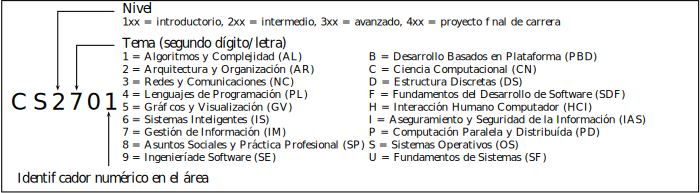
\includegraphics[width=13cm]{\OutputFigsDir/course-coding}
      \caption{Esquema de codificación para los cursos.}\label{fig:course-coding}
      \end{figure}
\end{latexonly}
\begin{htmlonly}
      \begin{rawhtml}
            <p>
                  <img src="./figs/course-coding.png" style="width: 13cm; height: 5cm;">
            </p>
      \end{rawhtml}
\end{htmlonly}

El tipo de curso esta determinado por sus 2 primeras letras. Los posibles códigos para estos tipos son:
\input{\OutputTexDir/prefix-description-ES}

Al mismo tiempo, y de acuerdo a la ley universitaria vigente, los cursos están clasificados en:
\begin{inparadesc}
\item [AF:] Área formativa,
\item [AE:] Área de especialidad,
\item [AB:] Área básica,
\item [AC:] Área complementaria.
\end{inparadesc}

% Table of courses by semesters
\begin{landscape}
\section{Estructura Curricular}\label{sec:courses-by-semester}
La relación de cursos se muestra a continuación:
\input{\OutputTexDir/tables-by-semester-\LANG}

\OnlyPeruSPC{Es importante resaltar que todos los semestres podrían ser completados con cursos extras de acuerdo al perfil de la institución.}
\end{landscape}



\begin{landscape}
\section{Distribución de tópicos por curso}\label{sec:topics-by-course}
Las siguientes tablas nos muestran la distribución de todos los tópicos del 
cuerpo del conocimiento de \ac{\currentarea} en todos los cursos.
\section{Distribución de tópicos por curso}\label{sec:topics-by-course}
Las siguientes tablas nos muestran la distribución de todos los tópicos del 
cuerpo del conocimiento de \ac{\currentarea} en todos los cursos.
\input{\OutputTexDir/topics-by-course}
\section{Resultados esperados distribuídos por curso}\label{sec:outcomes-by-course}
Las siquientes tablas nos muestras una visión global de los resultados que se esperan lograr en cada 
curso de la presente malla curricular. 
La lista completa de resultados esperados se encuentra en la Sección:~\ref{sec:outcomes}.
\section{Resultados esperados distribuídos por curso}\label{sec:outcomes-by-course}
Las siquientes tablas nos muestras una visión global de los resultados que se esperan lograr en cada 
curso de la presente malla curricular. 
La lista completa de resultados esperados se encuentra en la Sección:~\ref{sec:outcomes}.
\input{\OutputTexDir/outcomes-by-course}

\section{Malla curricular}\label{sec:vision-grafica}
\vspace{-0.3cm}
Este documento también puede ser analizado desde el punto de vista 
de los prerequisitos de forma gráfica.

\begin{latexonly}
      \begin{figure}[H]
            \includegraphics[width=23cm]{\OutputFigsDir/small-graph-curricula-ES.ps}
            \label{fig:malla-curricular}
            \caption{Malla curricular \SchoolFullName}
      \end{figure}
\end{latexonly}
\begin{htmlonly}
      \begin{rawhtml}
            <div class="center">
                  <iframe scrolling="no" frameborder="0" src="./figs/big-graph-curricula-<LANG_PREFIX>.svg" width="1916pt" height="1218pt">
                  <p><b>This browser is not able to show SVG: try Firefox, Chrome, Safari, or Opera instead.</b></p>
                  </iframe>
            </div>
      \end{rawhtml}
\end{htmlonly}

\end{landscape}

\section{Cursos por resultado ({\it Outcome})}\label{sec:courses-by-outcome}
\input{\OutputTexDir/courses-by-outcome-\LANG}




\section{Distribución de cursos en la carrera}
Esta propuesta puede ser analizada por el número de créditos dedicados a cada área
%horas de clase de las mismas
y por niveles de cursos (Introductorios, Intermedios, Avanzados y Proyectos).
\vspace{0.5cm}

\begin{figure}[h!]
      \centering
      \includegraphics[width=10cm]{\OutputFigsDir/pie-credits}
      \label{fig:pie-credits}
      \caption{Distribución de cursos por áreas considerando creditaje.}
\end{figure}

% \input{\OutputTexDir/distribution-area-by-semester}
\input{\OutputTexDir/distribution-credits-by-area-by-semester}

\begin{figure}[h!]
      \centering
      \includegraphics[width=10cm]{\OutputFigsDir/pie-by-levels}
      \label{fig:pie-niveles}
      \caption{Distribución de créditos por niveles de cursos.}
\end{figure} %Graphics by level, by area, etc

\section{Compatibilidad de la carrera con relación a estandares internacionales}
En esta sección presentamos la distribución de cursos por áreas de concentración en 
contraste con las propuestas internacionales de las carreras de la \textit{Computing Curricula} 
de \htmladdnormallink{IEEE-CS}{http://www.computer.org}/\htmladdnormallink{ACM}{http://www.acm.org}.

Es necesario notar que \underline{en algunos casos las materias podrían aparecen en más de un eje} 
pues tienen contenido de más de una área. 
Por ejemplo, la materia de sistemas operativos contiene unidades de aplicación 
que pueden ser clasificadas en Tecnología de Información pero al mismo tiempo contiene fundamentos 
de como está estructurado un Sistema Operativo que es del eje de Ciencia de la Computación. 
En estos casos el creditaje ha sido divido entre los ejes correspondientes.
\input{\OutputTexDir/list-of-courses-per-area}

Considerando esta distribución, las figuras~\ref{fig:comparing-curves-\currentarea-\currentinstitution-with-CE} 
a la~\ref{fig:comparing-curves-\currentarea-\currentinstitution-with-SE} 
nos permiten tener una visión gráfica de esta malla curricular frente a las propuestas de 
carreras presentadas por \htmladdnormallink{IEEE-CS}{http://www.computer.org}/\htmladdnormallink{ACM}{http://www.acm.org} en la \textit{Computing Curricula}
\input{\OutputTexDir/comparing-with-standards-\LANG}

\chapter{Plan de estudios \YYYY}\label{chap:GeneralInfo} 

\section{Clasificación de los cursos por niveles}
De acuerdo a la \textit{Computing Curricula}, los cursos son clasificados en 3 niveles: Introductorios (Códigos 100), 
Intermedios  (Códigos 2..), Avanzados  (Códigos 3..) y orientados a la construcción del trabajo de final de carrera  (Códigos 4..) también llamado tesis.

Los cursos de tercer nivel tienen por objetivo abrir varias posibilidades de especialización a través de cursos electivos

Esta propuesta de malla curricular está basada en el abordaje orientado a objetos. 
El abordaje orientado a la web se escogió porque hacia eso apuntan las tendencias 
futuras de la computación.

\section{Codificación de los cursos}
Los cursos se encuentran codificados bajo el esquema que se muestra en la Figura~\ref{fig:course-coding}:

\begin{latexonly}
      \begin{figure}[ht]
      \centering
      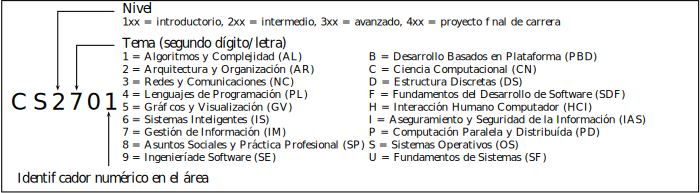
\includegraphics[width=13cm]{\OutputFigsDir/course-coding}
      \caption{Esquema de codificación para los cursos.}\label{fig:course-coding}
      \end{figure}
\end{latexonly}
\begin{htmlonly}
      \begin{rawhtml}
            <p>
                  <img src="./figs/course-coding.png" style="width: 13cm; height: 5cm;">
            </p>
      \end{rawhtml}
\end{htmlonly}

El tipo de curso esta determinado por sus 2 primeras letras. Los posibles códigos para estos tipos son:
\input{\OutputTexDir/prefix-description-ES}

Al mismo tiempo, y de acuerdo a la ley universitaria vigente, los cursos están clasificados en:
\begin{inparadesc}
\item [AF:] Área formativa,
\item [AE:] Área de especialidad,
\item [AB:] Área básica,
\item [AC:] Área complementaria.
\end{inparadesc}

% Table of courses by semesters
\begin{landscape}
\section{Estructura Curricular}\label{sec:courses-by-semester}
La relación de cursos se muestra a continuación:
\input{\OutputTexDir/tables-by-semester-\LANG}

\OnlyPeruSPC{Es importante resaltar que todos los semestres podrían ser completados con cursos extras de acuerdo al perfil de la institución.}
\end{landscape}



\begin{landscape}
\section{Distribución de tópicos por curso}\label{sec:topics-by-course}
Las siguientes tablas nos muestran la distribución de todos los tópicos del 
cuerpo del conocimiento de \ac{\currentarea} en todos los cursos.
\section{Distribución de tópicos por curso}\label{sec:topics-by-course}
Las siguientes tablas nos muestran la distribución de todos los tópicos del 
cuerpo del conocimiento de \ac{\currentarea} en todos los cursos.
\section{Distribución de tópicos por curso}\label{sec:topics-by-course}
Las siguientes tablas nos muestran la distribución de todos los tópicos del 
cuerpo del conocimiento de \ac{\currentarea} en todos los cursos.
\input{\OutputTexDir/topics-by-course}
\section{Resultados esperados distribuídos por curso}\label{sec:outcomes-by-course}
Las siquientes tablas nos muestras una visión global de los resultados que se esperan lograr en cada 
curso de la presente malla curricular. 
La lista completa de resultados esperados se encuentra en la Sección:~\ref{sec:outcomes}.
\section{Resultados esperados distribuídos por curso}\label{sec:outcomes-by-course}
Las siquientes tablas nos muestras una visión global de los resultados que se esperan lograr en cada 
curso de la presente malla curricular. 
La lista completa de resultados esperados se encuentra en la Sección:~\ref{sec:outcomes}.
\section{Resultados esperados distribuídos por curso}\label{sec:outcomes-by-course}
Las siquientes tablas nos muestras una visión global de los resultados que se esperan lograr en cada 
curso de la presente malla curricular. 
La lista completa de resultados esperados se encuentra en la Sección:~\ref{sec:outcomes}.
\input{\OutputTexDir/outcomes-by-course}

\section{Malla curricular}\label{sec:vision-grafica}
\vspace{-0.3cm}
Este documento también puede ser analizado desde el punto de vista 
de los prerequisitos de forma gráfica.

\begin{latexonly}
      \begin{figure}[H]
            \includegraphics[width=23cm]{\OutputFigsDir/small-graph-curricula-ES.ps}
            \label{fig:malla-curricular}
            \caption{Malla curricular \SchoolFullName}
      \end{figure}
\end{latexonly}
\begin{htmlonly}
      \begin{rawhtml}
            <div class="center">
                  <iframe scrolling="no" frameborder="0" src="./figs/big-graph-curricula-<LANG_PREFIX>.svg" width="1916pt" height="1218pt">
                  <p><b>This browser is not able to show SVG: try Firefox, Chrome, Safari, or Opera instead.</b></p>
                  </iframe>
            </div>
      \end{rawhtml}
\end{htmlonly}

\end{landscape}

\section{Cursos por resultado ({\it Outcome})}\label{sec:courses-by-outcome}
\input{\OutputTexDir/courses-by-outcome-\LANG}




\section{Distribución de cursos en la carrera}
Esta propuesta puede ser analizada por el número de créditos dedicados a cada área
%horas de clase de las mismas
y por niveles de cursos (Introductorios, Intermedios, Avanzados y Proyectos).
\vspace{0.5cm}

\begin{figure}[h!]
      \centering
      \includegraphics[width=10cm]{\OutputFigsDir/pie-credits}
      \label{fig:pie-credits}
      \caption{Distribución de cursos por áreas considerando creditaje.}
\end{figure}

% \input{\OutputTexDir/distribution-area-by-semester}
\input{\OutputTexDir/distribution-credits-by-area-by-semester}

\begin{figure}[h!]
      \centering
      \includegraphics[width=10cm]{\OutputFigsDir/pie-by-levels}
      \label{fig:pie-niveles}
      \caption{Distribución de créditos por niveles de cursos.}
\end{figure} %Graphics by level, by area, etc

\section{Compatibilidad de la carrera con relación a estandares internacionales}
En esta sección presentamos la distribución de cursos por áreas de concentración en 
contraste con las propuestas internacionales de las carreras de la \textit{Computing Curricula} 
de \htmladdnormallink{IEEE-CS}{http://www.computer.org}/\htmladdnormallink{ACM}{http://www.acm.org}.

Es necesario notar que \underline{en algunos casos las materias podrían aparecen en más de un eje} 
pues tienen contenido de más de una área. 
Por ejemplo, la materia de sistemas operativos contiene unidades de aplicación 
que pueden ser clasificadas en Tecnología de Información pero al mismo tiempo contiene fundamentos 
de como está estructurado un Sistema Operativo que es del eje de Ciencia de la Computación. 
En estos casos el creditaje ha sido divido entre los ejes correspondientes.
\input{\OutputTexDir/list-of-courses-per-area}

Considerando esta distribución, las figuras~\ref{fig:comparing-curves-\currentarea-\currentinstitution-with-CE} 
a la~\ref{fig:comparing-curves-\currentarea-\currentinstitution-with-SE} 
nos permiten tener una visión gráfica de esta malla curricular frente a las propuestas de 
carreras presentadas por \htmladdnormallink{IEEE-CS}{http://www.computer.org}/\htmladdnormallink{ACM}{http://www.acm.org} en la \textit{Computing Curricula}
\input{\OutputTexDir/comparing-with-standards-\LANG}

%%%%%%%%%%%%%%%%%%%%%%%%%%%%%%%%%%%%%%%%%%%%%%%%%%%%%%%%%%%%%%%%%%%%%%%%%%%%%%%

\begin{btSect}[apalike]{curricula-main}
\section*{\BibliographySection}
\btPrintCited
\end{btSect}
\end{btUnit}
  
\chapter{Contenido detallado por curso}\label{chap:syllabi}
\input{\OutputTexDir/list-of-syllabi}

\OnlyPeruUCSP{\begin{landscape}
\chapter{Equivalencias con otros planes curriculares}\label{chap:equivalence}
A continuación se pueden observar las equivalencias de la presente malla con el(los) Plan(es) curricular(es) anterior(ES). 
Para ver mayores detalles de la malla propuesta observar la sección~\ref{sec:courses-by-semester} Pág.~\pageref{sec:courses-by-semester}.

\input{\OutputTexDir/equivalences}
\end{landscape}

}
 
\chapter{Laboratorios}\label{chap:laboratories}
\input{\OutputTexDir/laboratories-by-course}

\OnlyPeruSPC{
\chapter{Profesores \& Cursos}\label{chap:professors-and-courses}
\input{\OutputTexDir/courses-by-professor-\LANG}

\input{\OutputTexDir/professor-by-course-\LANG}
}
\OnlyPeruMINEDU{
\chapter{Profesores \& Cursos}\label{chap:professors-and-courses}
\input{\OutputTexDir/courses-by-professor-\LANG}

\input{\OutputTexDir/professor-by-course-\LANG}
}

\OnlyPeruSPC{\chapter{Resultados específicos por curso}\label{sec:specific-outcomes-by-course}
%\input{\OutputTexDir/list-of-courses-by-specific-outcome-\LANG}
\begin{landscape}
\input{\OutputTexDir/table-of-courses-by-specific-outcome-\LANG}
\end{landscape}
}

\OnlyPeruMINEDU{\chapter{Resultados específicos por curso}\label{sec:specific-outcomes-by-course}
%\input{\OutputTexDir/list-of-courses-by-specific-outcome-\LANG}
\begin{landscape}
\input{\OutputTexDir/table-of-courses-by-specific-outcome-\LANG}
\end{landscape}
}
